% !TeX encoding = UTF-8
% !TeX program = xelatex
% !TeX spellcheck = en_US

\documentclass[doctor,english,pdf]{ustcthesis}
% doctor|master|bachelor [academic|professional] [chinese|english] [print|pdf]
% [super|numebers|authoryear]

\title{基于ATLAS探测器上ZZ玻色子到全轻子通道的衰变事例对标准模型ZZ过程和寻找重共振态衰变到双Z玻色子过程的研究}
\author{祝鹤龄}
\major{粒子与原子核物理}
\supervisor{赵政国}
\cosupervisor{马宏}
% \date{二〇一七年五月一日} % 注释掉则为今日
% \professionaltype{专业学位类型}
% \secretlevel{秘密}        % 绝密|机密|秘密,注释本行则不保密
% \secretyear{20}           % 保密年限

\entitle{Studies of Standard Model ZZ Production and Search for heavy ZZ resonances in Purely Leptonic Decay with ATLAS Detector}
\enauthor{Heling Zhu}
\enmajor{Particle and Nuclear Physics}
\ensupervisor{Zhengguo Zhao}
\encosupervisor{Hong Ma}
% \endate{May 1, 2017}      % Today if commented
% \enprofessionaltype{Professional degree type}
% \ensecretlevel{Secret}    % Top secret|Highly secret|Secret


% 加载宏包和配置
\usepackage{graphicx}
\graphicspath{{figures/}}
\usepackage{booktabs}
\usepackage{longtable}
\usepackage[ruled,linesnumbered]{algorithm2e}
\usepackage{siunitx}
\usepackage{amsthm}
\usepackage{hyperref}
\usepackage{setspace}
\usepackage{tabularx}
\usepackage{bigstrut}

%% sepecial defination for ATLAS
\usepackage{main-defs}
\usepackage{latex/atlasunit}
\usepackage{latex/atlasparticle}
\usepackage{latex/atlasjournal}
\usepackage{latex/atlasmisc}
\usepackage{latex/atlasphysics}

\DeclareRobustCommand\cs[1]{\texttt{\char`\\#1}}
\newcommand\pkg{\textsf}

\renewcommand\vec{\symbf}
\newcommand\mat{\symbf}
\newcommand\ts{\symbfsf}
\newcommand\real{\mathbf{R}}
\newcommand{\doi}[1]{\href{http://dx.doi.org/#1}{\nolinkurl{#1}}}

% Added by Tao for testing
% \setmainfont{TeX Gyre Termes}
% \setsansfont{TeX Gyre Heros}
% \setCJKmainfont[AutoFakeBold,ItalicFont=FandolKai]{FandolSong}
% \setCJKfamilyfont{zhkai}[AutoFakeBold]{FandolKai}
% \setCJKsansfont[AutoFakeBold]{FandolHei}
% \setCJKfamilyfont{zhsong}[AutoFakeBold]{FandolSong}
% \setCJKfamilyfont{zhhei}[AutoFakeBold]{FandolHei}
% \setmonofont[Scale=MatchLowercase]{DejaVu Sans Mono}

%\geometry{left=2cm,right=2cm}
\begin{document}

\maketitle
%\makestatement

\frontmatter
% !TeX root = ../main.tex

\begin{abstract}
  中文摘要
\end{abstract}

\begin{enabstract}
  English abstract.

\end{enabstract}

% !TeX root = ../main.tex

\begin{acknowledgments}

First of all, I would like to express my great gratitude to my supervisors Prof. Zhao Zhengguo and Dr. Ma Hong, for their guidance and patience during my Ph.D years.
It's Zhengguo, who inspire me with his deep physics insight when I was an undergraduate student and led me enter the field of Particle Physics.
I will never forget how I was attracted by his broad knowledge and the amazing picture of particles he showed me, which became the reason I choose the Particle Physics as my major.
It's always relaxed and benificial greatly when chating with him, which broads my version, makes me to be more confident and helps me step out of so many difficulties.

Thanks to Hong, for giving me the oppotunity to study in Brookhaven National Lab (BNL) that I can work with so many senior and brilliant physicists, and teaching me a lot in the details of physics.
As the chair of physics department at BNL, can you imagine that he managed to take time sitting with me every week, teaching me the details and techniques of my analysis
as well as helping me to parepre my talks at conference.

Thank you both for leading me to the field of physics, showing me how beautiful the science and the world are. 
And thank you for providing me so many oppotunities and tremendous supports to work at physics frontier and work with people all over the world.
It's my greatest honor to be your student.
Your strong personalitis will definitely influence my future life and career.

I would like to give my large gratitude to Prof. Zhou Bing.
It's Bing who introduced me to ATLAS experiment when I was a junior. 
As a professor and group leader of ATLAS group in University of Michigan with busy schedule, 
Bing still took time to teach me in physics start from simple formulas and help me to prepare my first academic presentation patiently when I was a undergraduate student.
Also it's my great fortune that I can have opportunities to work with you and learn from you in so many analyses during these years.
Your kind and patience, your high standard influence me deeply in all these years.

Moreover, I really want to give my sincere gratitude to Dr. Xu Lailin.
Thank you, Lailin, for all your helps during the passing five years.
Thanks for teaching me in all the analysis details, coding techniques, presentation skills hand by hand.
You are really a very good and patient teacher and give me as many knowledges as you can.
Your broad knowledge, your perseverance in science and your very hard working indeed affect me a lot.

In the meantime, I want to give my special thanks to Dr. Li Bing, who helped me a lot in several different analyses 
(low-mass 4$\mu$ resonance search, VBSZZ analysis, $Z'$ search), he never hesitated to give his hand to me when I faced difficulties.

I would like to express my gratitude to many colleagues in both USTC and BNL team.
Thanks to Prof. Sun Yongjie, who is the supervisor of my undergraduate thesis, helped me start my first detector project on MRPC. 
Also thanks Dr. Liu Zhen who taught me in details in this project, and helped me a lot for my life at BNL too.
Thanks to Prof. Peng Haiping, Prof. Zhu Yingchun and Dr. Hu Qipeng for helping me all the details and techniques in HWW analysis when I was a biginner.
Thanks to Dr. Dai Tiesheng, I have learnt quite a lot in the project of Monitored Drift Tubes (MDT) when working with you at CERN and also thank you for all the help in regular life since that was my first time to Europe.
Thanks to Dr. Chen Hucheng, who is the supervisor of my ATLAS qualification task on LAr Trigger Digitizer Boards (LTDB) and the person lead me into this interesting electronic project.
And my appreciation to Dr. Xu Hao, Dr. Chen Kai and Dr. Liu Hongbin who taught me in patience for this project as I was really a freshman on electronics.
Thanks to Prof. Yuji Enari and Dr. Georges Aad for the help in LAr software tasks when I moved from BNL to CERN.
In the meantime, I would really like to give my gratitude to Dr. Michael Begal, Dr. Marc-Andre Pleier, Dr. Alessandro Tricoli, Dr. George Redlinger, Dr. Viviana Cavaliere, Dr. Gaetano Barone and many senior physicists in BNL omaga group. 
I have learnt a lot from every chat with you and every seminar you hosted.
Also I want to thanks to Prof. Wu Yusheng, Prof. Qian Jianming, Prof. Liu Yanwen, Dr. Ju Xiangyang for teaching me in lots of details in different physics analyses.

Moreover, I want to give my thanks to friends I met at USTC, BNL and CERN during my Ph.D years.
Thanks to Dr. Yang Qian, Dr. Chu Xiaoxuan, Dr. Tu Biao, Dr. Gao Shanshan, Dr. Liu Feng, Dr. Yuan Guangyuan, and many other friends I met at BNL. 
Thanks to Prof. Geng Cong, Dr. Li Peilian, Dr. Zhang Liqing, Dr. Guo Yicheng, Dr. Xu Tairan, Dr. Wang Rongkun, Chen Jing, He Fudong, Guo Qianying, Chen Ye, Xu Hao, Wang Tao, Xie Xiangyu, Liu Xiangtian and all friends I met at USTC and CERN. 
Thank you all my friends! I will always remember all the happiniess with you, and best wishes to you in the future!

Last but not least, I would give my greatest gratitude to my families. Thanks my parents for giving me all your endless loves and supports in my whole life.
My deep appreciation to my three aunts for loving and caring me so much since I was born and help me to accompany with my mother when I was thousands miles far away from home.
And my husband, Lin, thank you for your understanding and walk through all difficulties with me in these years especially when we were in a foreign country.

\end{acknowledgments}

\tableofcontents
\listoffigures
\listoftables

\makededicate
\newpage

\mainmatter
% !TeX root = ../main.tex

\chapter{Introduction}

The goal of particle physics is to understand how our universe works at its most fundamental level. It can be accomplished by pursuing the mysteries of the basic construction of matter and energy, probing the interactions between elementary particles, and exploring the basic nature of space and time itself. 

\textbf{Elementary particles}

From around the 6th century BC, ancient Greek philosophers Leucippus, Democritus, and Epicurus brought up a philosophical idea that everything is composed of “uncuttable” elementary particles. In the 19th century, John Dalton, through his work on stoichiometry, concluded that each element of nature was composed of a single, unique type of particle. The particle was named as “atom” after the Greek word atomos, with the meaning of “indivisible”. However this Dalton’s atom theory was strongly challenged later. Near the end of 19th century, physicists discovered that Dalton's atoms are not, in fact, the fundamental particles of nature, but conglomerates of even smaller particles. Electron was discovered by J. J. Thomson in 1897, and then its charge was carefully measured by Robert Andrews Millikan and Harvey Fletcher in their "oil drop experiment" of 1909. In early 20th-century, Rutherford's "gold foil experiment" showed that the atom is mainly empty space, with almost all its mass concentrated in a tiny positive charge atomic nucleus. Then the discoveries of anti-particles (the positron in 1932) and other particles (e.g. the muon in 1936) shows that more discoveries could be expected in future experiments.

Starting from 1950s, more accelerator facilities were put into service. Throughout the 1950s and 1960s, a bewildering variety of particles were found in collisions of particles from increasingly high-energy beams. It was referred to informally as the "particle zoo".
In 1964, the quark model was independently proposed by physicists Murray Gell-Mann and George Zweig, and experimentally confirmed of their existence in mid-1970s. In 1970s, the establishment of quantum chromodynamics  (QCD) postulated the fundamental strong interaction, experienced by quarks and mediated by gluons.

The well-known Standard model (SM) was developed in stages throughout the latter half of the 20th century. Since then, confirmation of the top quark (1995), the tau neutrino (2000), and the Higgs boson (2012) have added further credence to the Standard Model.
Now, the quarks, leptons and gauge bosons are the elementary constituents in a framework of Standard Model of particle physics, which theoretically describes three of the four known fundamental forces (the electromagnetic, weak, and strong interactions, and not including the gravitational force) in the universe, as well as classifies all known elementary particles.

\textbf{Higgs mechanics and electroweak symmetry breaking}

In 1961, Sheldon Glashow brought forward a unified electroweak theory to combine the electromagnetic and weak interactions. In the standard model, at energy high enough that electroweak symmetry is unbroken, all elementary particles are massless. But measurements show the fact that the W and Z bosons actually have masses. Later on, the Higgs mechanics resolves this conundrum. The simplest description of the mechanism adds a Higgs field that permeates all space to the Standard Model. Below some extremely high energy, the field causes spontaneous symmetry breaking during interactions. All massive particles in the Standard Model, including the W and Z bosons, interact with Higgs boson to acquire their mass.

Over the past few decades, the combination of electroweak theory, Higgs mechanics and strong interactions has been widely accepted. But the Higgs boson, which is essential to explain the mechanics of the property "mass" for gauge bosons and fermions, had been the final missing piece in the Standard Model of particle physics for the time being. The mass of Higgs boson was not be specifically predicted, and it has been searched in several large experiments (eg. LEP at CERN, Tevatron at Fermilab, and LHC at CERN). In 2012, the discovery of Higgs boson was finally announced by the ATLAS and CMS collaborations at the Large Hadron Collider (LHC) with its mass round 125 GeV. Peter Higgs and Francois Englert were award the 2013’s Nobel Prize in Physics for their theoretical discovery of a mechanism that contributes to our understanding of the origin of mass of subatomic particles.

\textbf{Contents of this thesis}

This thesis is organized as follows. Section 2 briefly introduces the Standard Model of particle physics, the Higgs mechanism related to the thesis and the LHC phenomenology. Section 3 gives an overview of the LHC and the ATLAS detector. The detector simulation and the reconstruction of physics objects are described in section 4. Section 5 focuses on the Standard model ZZ production cross section measurement in ZZ → 4l channel, and the observation of its electroweak component as well as its further prospects in High luminosity LHC (HL-LHC). Section 6 present the search of possible heavy Higgs in H → ZZ → 4l channel. In the end, section 7 gives the summary and outlook for future physics in LHC.



% !TeX root = ../main.tex

\chapter{Theory}

\section{The Standard Model of Particle Physics}
The standard model (SM) reflects our current understanding of elementary particles and several basic interactions.
It is a gauge quantum field theory containing the internal symmetries of the unitary product group $SU(3) \times SU(2) \times U(1)$, 
in which the color group $SU(3)$ presents the strong interaction, and $SU(2) \times U(1)$ describes the electroweak interactions.
Over the past decades, the SM has been widely tested through various experiments with extremely high precision.

\subsection{Elementary particles in the Standard Model}
\label{elementaryparticles}

The elementary particles in SM can be classified into 3 class: \textit{fermions}, \textit{gauge bosons} and the \textit{Higgs boson} as shown in Figure~\ref{fig:eleP-1}.
\begin{figure}[!htb]
  \centering
  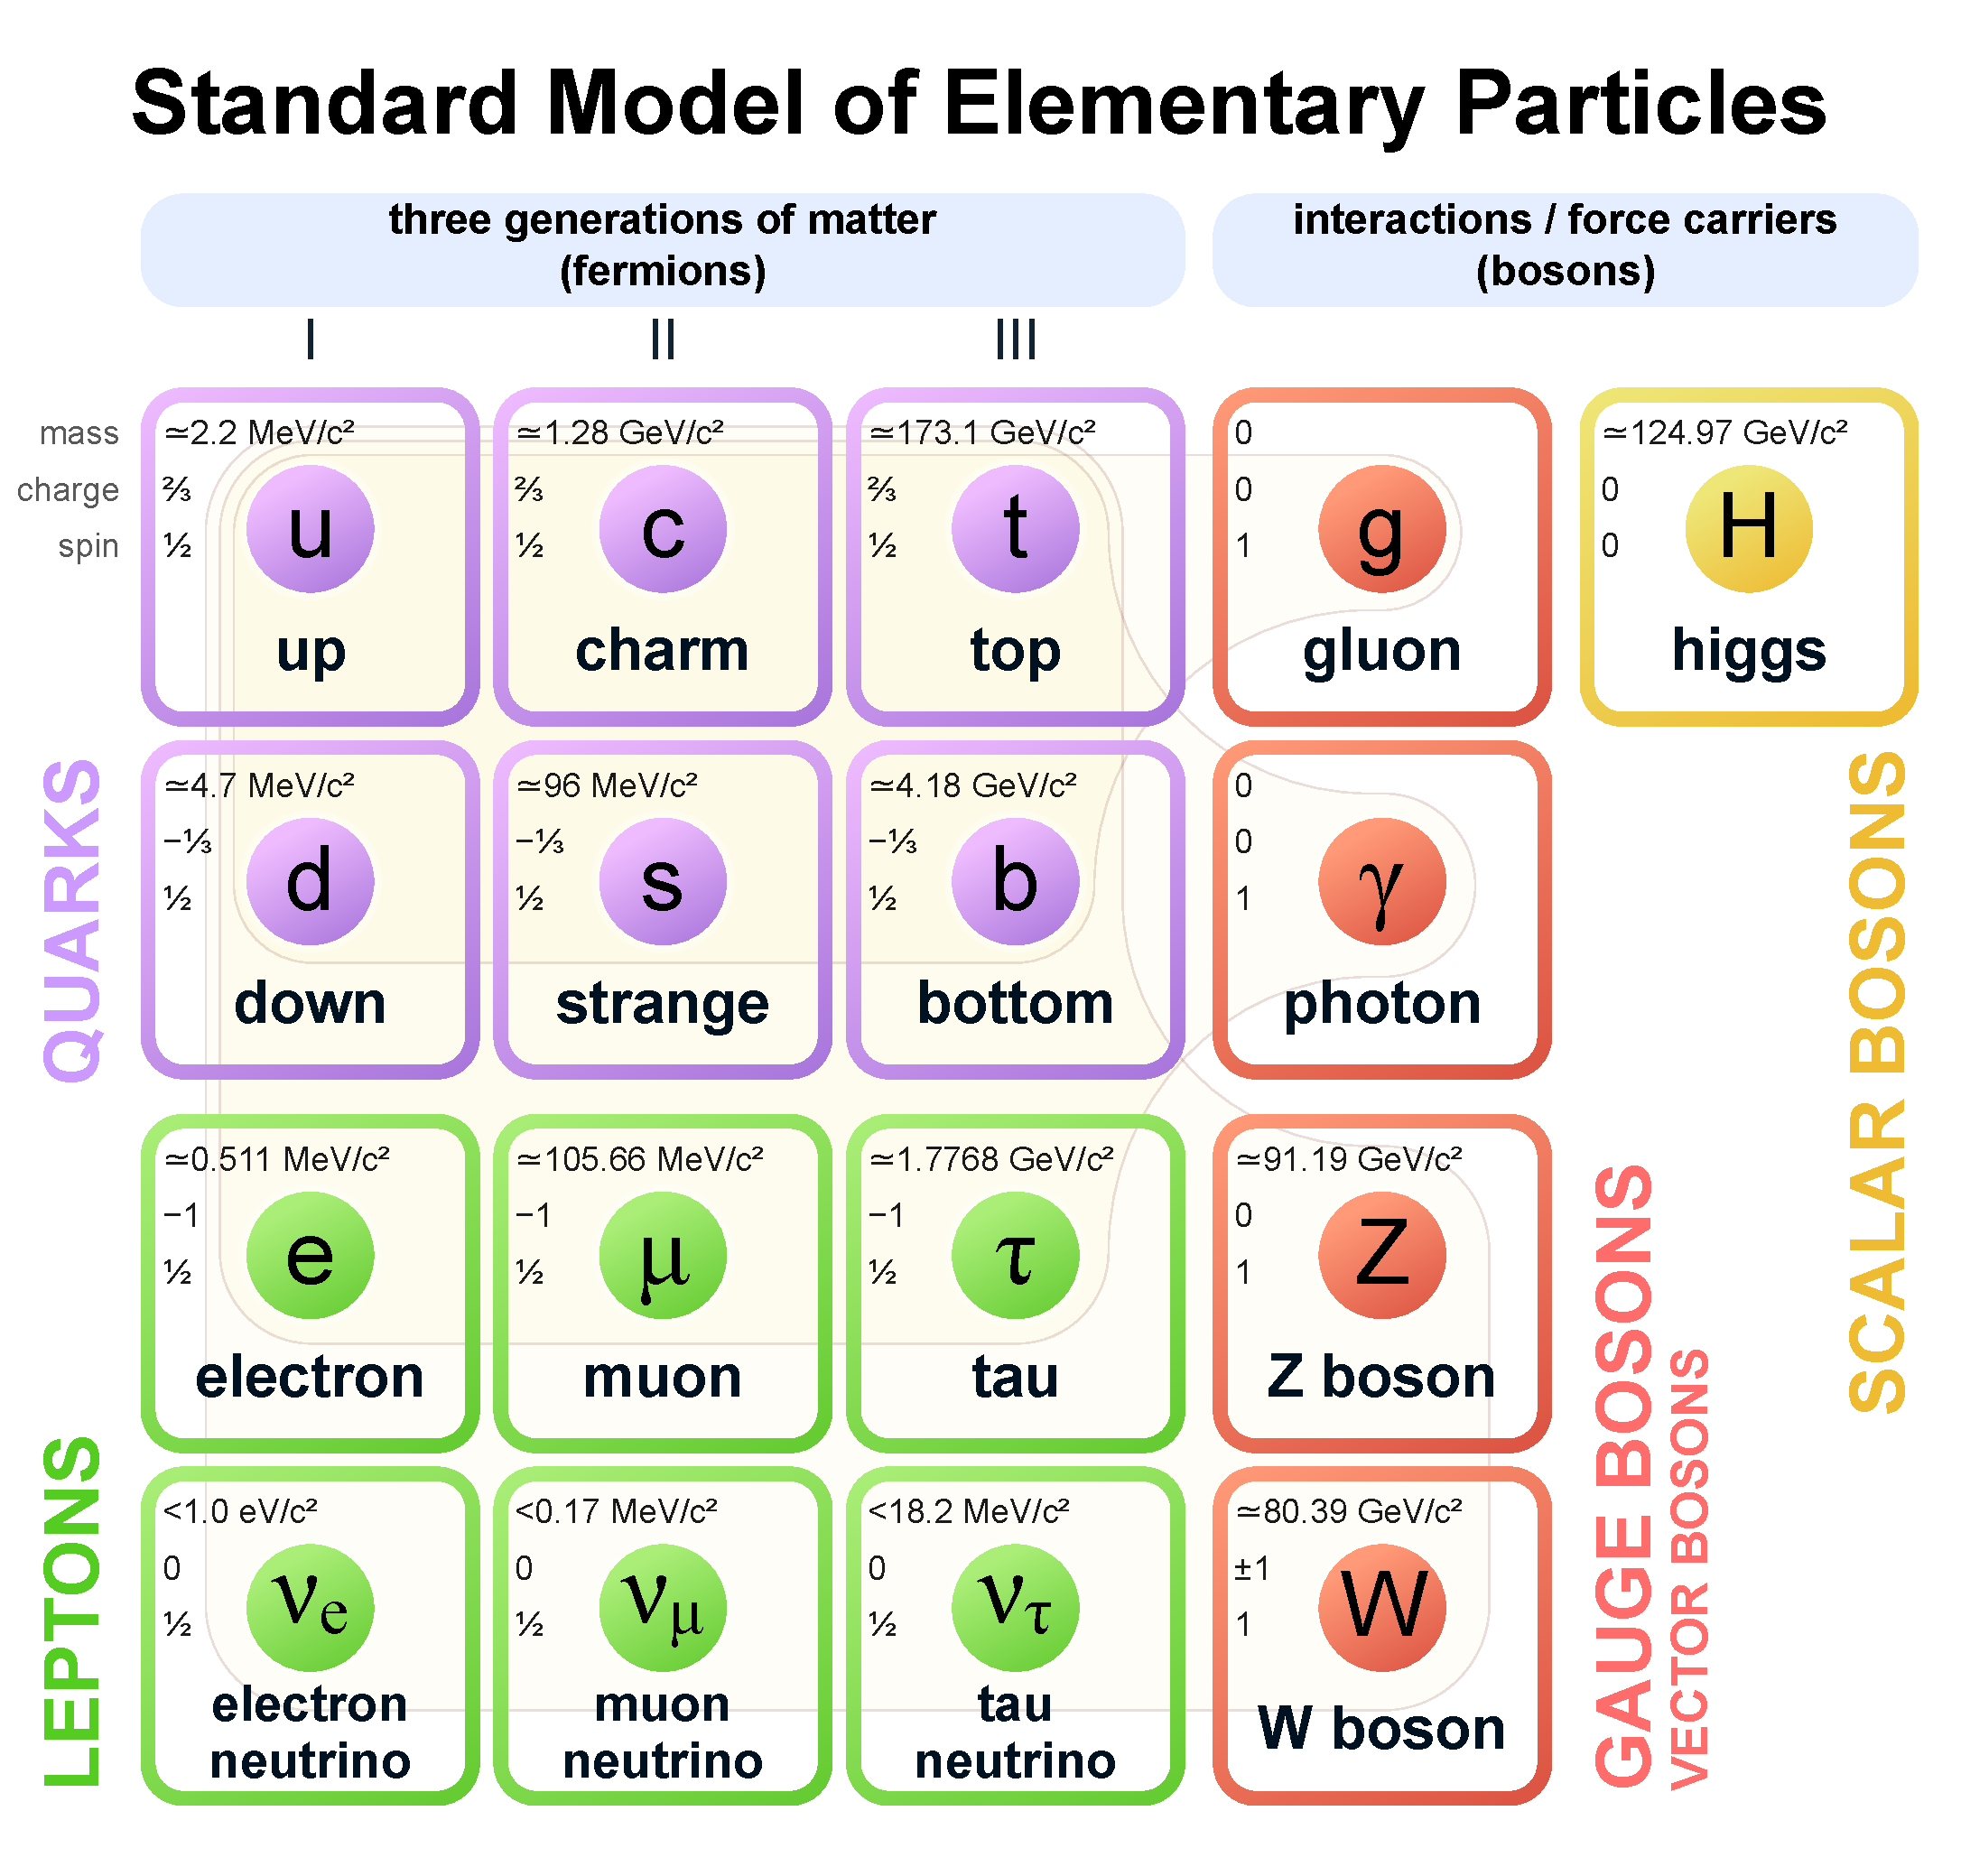
\includegraphics[width=0.7\textwidth]{figures/Theory/Standard_Model_of_Elementary_Particles.pdf}
  \caption{The elementary particles of the Standard Model.}
  \label{fig:eleP-1}
\end{figure}

\textbf{Fermions}
The Standard Model includes 12 elementary particles of spin-$\frac{1}{2}$ obeying the Fermy-Dirac statistics, known as fermions. 
They are classified into two types: \textit{leptons} and \textit{quarks} according to the their interactions.
The \textit{leptons} include three generations: electron ($e$) and electron neutrino ($\nu_{e}$); 
muon ($\mu$) and muon neutrino ($\nu_{\mu}$); tau ($\tau$) and tau neutrino ($\nu_{\tau}$).
The $e$, $\mu$ and $\tau$ carry electric charge of -1 and three neutrinos are electrically neutral. 
All the leptons can participate in electroweak interactions.
Also there are three generations of \textit{quarks}: up ($u$) and down ($d$); charm ($c$) and strange ($s$); top ($t$) and bottom ($b$).
The defining property of the quarks is that they carry color charge (while leptons don't), and hence interact via the strong interaction, 
letting them to be strongly bound from one to another, forming color-neutral composite 
particles (known as hadrons) containing either a quark and an antiquark (mesons) or three quarks (baryons).
In the meantime, $u$, $c$ and $t$ -quark carry electric charge of 2/3, and $d$, $s$ and $b$ -quark carry electric charge of -1/3. 
Hence they interact via all three interactions described in SM.
Each fermion also has its corresponding antiparticle.

\textbf{Gauge bosons}
act as force carriers that propagate the strong, weak, and electromagnetic interactions in SM.
They are spin-1 particles obeying the Bose-Einstein statistics. 
There are three types of gauge bosons:
\begin{itemize}
  \item The eight massless \textit{gluons} propagate the strong interactions between color charged particles (quarks).
  \item The massless \textit{photons} propagate the electromagnetic force between electrically charged particles.
  \item The $W^{+}$, $W^{-}$ and $Z$ bosons propagate the weak interactions between both quarks and leptons. All these three bosons are massive, the $W^{\pm}$ carries an electric charge of $+1$ and $−1$ and can also couple to the electromagnetic interaction while $Z$ boson is electrically neutral.
\end{itemize}
Figure~\ref{fig:eleP-2} shows the Feynman diagrams of corresponding interactions in SM.
\begin{figure}[!htb]
  \centering
  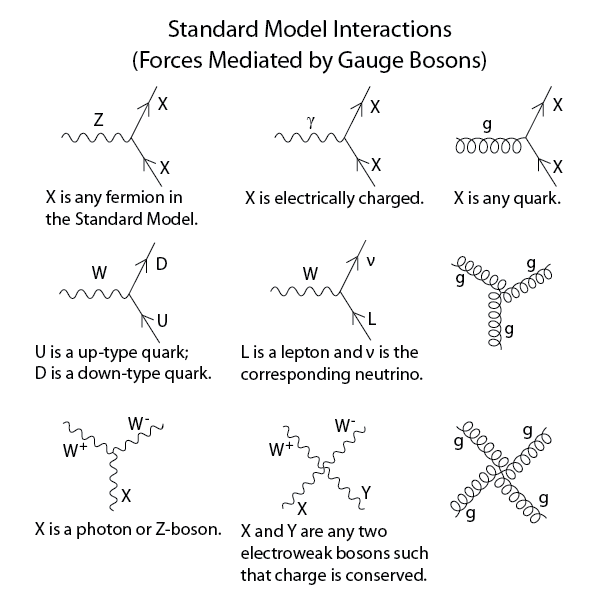
\includegraphics[width=0.8\textwidth]{figures/Theory/Standard_Model_Feynman_Diagram_Vertices.png}
  \caption{The Feynman diagrams of interactions mediated by gauge bosons that form the basis of the standard model.}
  \label{fig:eleP-2}
\end{figure}

\textbf{Higgs boson}
is a massive scaler elementary particle with spin-0. 
It plays a unique role in the SM by explaining the origin of masses of massive gauge bosons ($W^{\pm} and Z$) and fermions. 
And it is the last discovered particle in SM.

%\subsection{Elementary particles in the Standard Model}
\subsection{Electroweak theory}
\label{ewktheory}
The electroweak interaction is the unified description of two of the four known fundamental interactions of nature: electromagnetism and the weak interaction.
It is based on the gauge group of $SU(2)_{L} \times SU(1)_{Y}$, in which $L$ is the left-handed fields and $Y$ is the weak hypercharge \cite{Langacker:2009my}.
It follows the Lagrangian of
\begin{equation} \label{eq:Lew}
	L_{EW} = L_{gauge} + L_{Higgs} + L_{fermion} + L_{Yukawa}
\end{equation}

$L_{gauge}$ is the \textbf{gauge term} part
\begin{equation}
	L_{gauge} = -\frac{1}{4} W^{i}_{\mu\nu} W^{\mu\nu i} - \frac{1}{4} B_{\mu\nu} B^{\mu\nu}
\end{equation}
where $W^{i}_{\mu}$ and $B_{\mu}$ respectively present the $SU(2)_{L}$ and $SU(1)_{Y}$ gauge fields, with the corresponding field strength tensors of
\begin{equation}
\begin{split}
	& B_{\mu\nu} = \partial_{\mu} B_{\nu} - \partial_{\nu} B_{\mu} \\
	& W^{i}_{\mu\nu} = \partial_{\mu} W^{i}_{\nu} - \partial_{\nu} W^{i}_{\mu} - g \epsilon_{ijk} W^{j}_{\mu} W^{k}_{\nu}
\end{split}
\end{equation}
In the equations above, $g$ is the $SU(2)_{L}$ gauge coupling and $\epsilon_{ijk}$ is the totally antisymmetric tensor.
The gauge Lagrangian has three and four-point self interactions of $W^{i}$, which result in triple and quartic gauge boson couplings.

The second term of the Lagrangian is the \textbf{scaler part}:
\begin{equation} \label{eq:Lhiggs}
	{L}_{Higgs} = \left(D^{\mu}\phi\right)^{\dagger}D_{\mu}\phi - V(\phi)
\end{equation}
where $\phi = \binom{\phi^{+}}{\phi^{0}}$  is a complex Higgs scalar,
and $V(\phi)$ is the Higgs potential which is restricted into the form of 
\begin{equation} \label{eq:Vhiggs}
	V(\phi) = +\mu^{2}\phi^{\dagger}\phi + \lambda\left(\phi^{\dagger}\phi\right)^{2}
\end{equation}
due to the combination of $SU(2)_{L} \times SU(1)_{Y}$ invariance and renormalizability.
In Eq.~\ref{eq:Vhiggs}, $\mu$ is a mass-dependent parameter and $\lambda$ is the quartic Higgs scalar coupling, 
which represents a quartic self-interaction between the scalar fields.
When $\mu^{2} < 0$, there will be spontaneous symmetry breaking (more details in section~\ref{symbreaking}).
To maintain vacuum stability, $\lambda > 0$ is required.
And in Eq.~\ref{eq:Lhiggs}, the gauge covariant derivative is defined as
\begin{equation}
	D_{\mu}\phi = \left(\partial_{\mu} +ig\frac{\tau^{i}}{2}W_{\mu}^{i} + \frac{ig^{'}}{2}B_{\mu}\right)\phi
\end{equation}
in which $\tau^{i}$ represents the Pauli matrices, and $g'$ is the $U(1)_{Y}$ gauge coupling.
The square of the covariant derivative results in three and four-point interactions between the gauge and scalar fields.

The third term of the Lagrangian is the \textbf{fermion part}
\begin{equation} \label{eq:Lfermion}
\begin{split}
  	{L}_{fermion} = \sum_{m=1}^{F} & ( \bar{q}_{mL^{i}}^{0}\gamma_{\mu}D_{\mu}q_{mL}^{0} + \bar{l}_{mL^{i}}^{0}\gamma_{\mu}D_{\mu}l_{mL}^{0} + \bar{u}_{mR^{i}}^{0}\gamma_{\mu}D_{\mu}u_{mR}^{0} \\
  	& + \bar{d}_{mR^{i}}^{0}\gamma_{\mu}D_{\mu}d_{mR}^{0} + \bar{e}_{mR^{i}}^{0}\gamma_{\mu}D_{\mu}e_{mR}^{0} + \bar{\nu}_{mR^{i}}^{0}\gamma_{\mu}D_{\mu}\nu_{mR}^{0})
\end{split}
\end{equation} 
In Eq.~\ref{eq:Lfermion}, m is the family index of fermions, F is the number of families.
The subscripts $L (R)$ stand for the left (right) chiral projection $\psi_{L(R)} \equiv \left(1 \mp \gamma_{5} \right) \psi/2$.
\begin{equation}
	q_{mL}^{0} = \binom{u_{m}^{0}}{d_{m}^{0}}_{L}   \qquad    l_{mL}^{0} = \binom{\nu_{m}^{0}}{e_{m}^{-0}}_{L}
\end{equation}
are the $SU(2)$ doublets of left-hand quarks and leptons, while 
$u_{mR}^{0}$, $d_{mR}^{0}$, $e_{mR}^{-0}$ and $\nu_{mR}^{0}$ are the right-hand singlets.

The last term in Eq.~\ref{eq:Lew} is \textbf{Yukawa term}
\begin{equation}
\begin{split}
	{L}_{Yukawa} =& -\sum_{m,n=1}^{F} [\Gamma_{mn}^{u}\bar{q}_{mL}^{0}\widetilde{\phi}u_{nR}^{0} + \Gamma_{mn}^{d}\bar{q}_{mL}^{0}\phi d_{nR}^{0} \\
	& + \Gamma_{mn}^{e}\bar{l}_{mn}^{0}\phi e_{nR}^{0} + \Gamma_{mn}^{\nu}\bar{l}_{mL}^{0}\widetilde{\phi}\nu_{nR}^{0}]+h.c.
\end{split}
\end{equation}
the matrices $\Gamma_{mn}$ refer to the Yukawa couplings between single Higgs doublet ($\phi$) and the various flavors of quarks (m) and leptons (n).


%\subsection{Electroweak theory}
\subsection{Higgs mechanism and Electroweak symmetry breaking}
\label{symbreaking}

As shown in previous subsection, the Lagrangian $L_{gauge}$ does not involve any mass term due to the requirement of gauge invariance.
So all the W and B bosons should be massless. But experimental observations show that the gauge bosons are massive.
Therefore, the gauge invariance must be broken spontaneously.
The Higgs field is introduced to break the $SU(2)_{L} \times U(1)_{Y}$ symmetry and
guage bosons and fermions can interact with Higgs filed to acquire their masses.
And this specific process is named \textit{Higgs mechanism} in SM.

The Higgs field $\phi$ is a doublet and can be written in a Hermitian basis as
\begin{equation}
	\phi = \binom{\phi^{+}}{\phi^{0}} = \frac{1}{\sqrt{2}} \binom{\phi_{1} - i\phi_{2}}{\phi_{3} - i\phi_{4}}
\end{equation}
where $\phi_{i} = \phi_{i}^{+}$ stand for four Hermitian field. 
In this new basis, the Higgs potential in Eq.~\ref{eq:Vhiggs} can be expressed as:
\begin{equation}
	V(\phi) = \frac{1}{2}\mu^{2}\left(\sum_{i=1}^{4}\phi_{i}^{2}\right) + \frac{1}{4}\lambda\left(\sum_{i=1}^{4}\phi_{i}^{2}\right)^{2}
\end{equation}
To simplify the situation, the axis in this four-dimensional space can be choosen to satisfied
~$\left<0\left| \phi_{i} \right|0\right> = 0$ for $i = 1, 2, 4$, and $<0\left| \phi_{3} \right|0> = v$. Thus,
\begin{equation}
	V(\phi) \rightarrow V(v) = \frac{1}{2}\mu^{2}v^{2} + \frac{1}{4}\lambda v^{4}
\end{equation}
The minimization of this potential depends on the sign of $\mu^{2}$ as shown in figure~\ref{fig:C2_Higgs_potential}.
When $\mu^{2} > 0$ the minimum occurs at $v = 0$, namely the vacuum is empty space and $SU(2)_{L} \times U(1)_{Y}$ symmetry is unbroken.
In the case of $\mu^{2} < 0$, the $v = 0$ symmetric point is no longer stable and the minimum occurs at nonzero value of 
$v = \left( -\mu^{2}/\lambda\right)^{1/2}$ which breaks the $SU(2)_{L} \times U(1)_{Y}$ symmetry.
\begin{figure}[!htb]
  \centering
  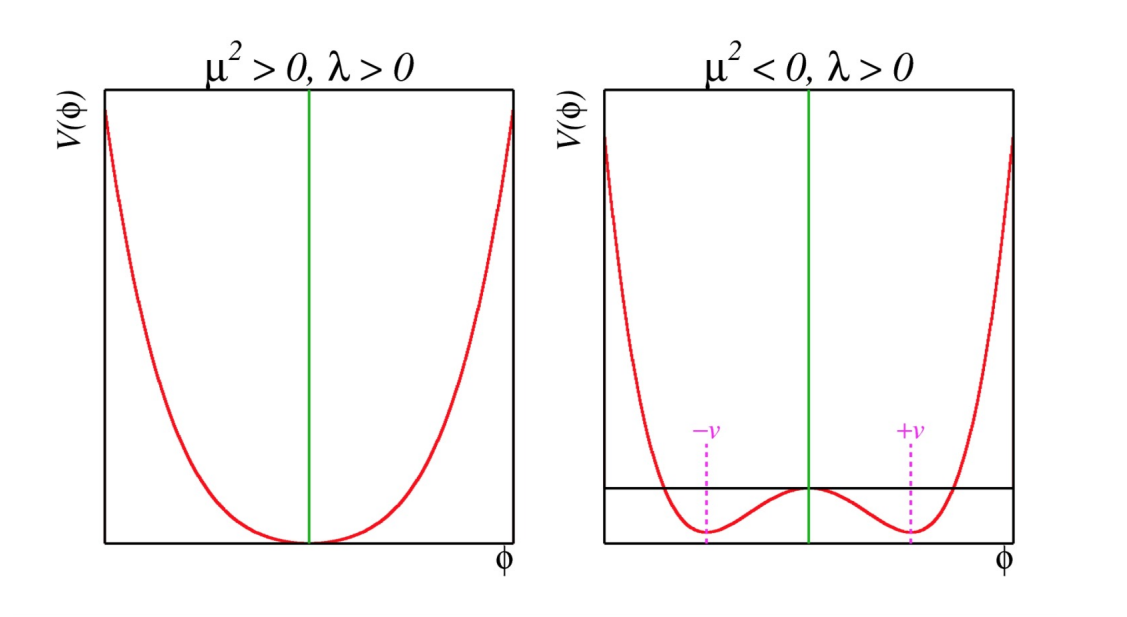
\includegraphics[width=0.7\textwidth]{figures/Theory/Vhiggs.png}
  \caption{Higgs potential $V(\phi)$ with $\mu^{2}>0$ (left) and $\mu^{2}<0$ (right).}
  \label{fig:C2_Higgs_potential}
\end{figure}
Thus, the classical vacuum $\phi_{0}$ of Higgs doublet can be expressed by
\begin{equation}
	\phi_{0} = \frac{1}{\sqrt{2}}\binom{0}{v}
\end{equation}
And to quantize around the classical vacuum in a general form:
\begin{equation}
	\phi = \frac{1}{\sqrt{2}} \binom{0}{v+H}
\end{equation}
Where H is a Hermitian field for physical Higgs scalar.
In this guage, the Lagrangian $L_{Higgs}$ in Eq.~\ref{eq:Lhiggs} takes a simple form
\begin{equation}
\begin{split} \label{eq:Lhiggs2}
	L_{Higgs} & = \left(D^{\mu}\phi\right)^{\dagger}D_{\mu}\phi - V(\phi) \\
	& = M_{W}^{2}W^{\mu+}W_{\mu}^{-}\left(1+\frac{H}{\nu}\right)^{2} + \frac{1}{2}M_{Z}^{2}Z^{\mu}Z_{\mu}\left(1+\frac{H}{\nu}\right)^{2} \\ 
        &   + \frac{1}{2}\left(\partial_{\mu}H\right)^{2} - V(\phi)
\end{split}
\end{equation}
where the W and Z fields are
\begin{equation}
\begin{split}
	& W^{\pm} = \frac{1}{\sqrt{2}} \left(W^{1} \mp iW^{2}\right) \\
	& Z = - sin\theta_{W}B + cos\theta_{W}W^{3}
\end{split}
\end{equation}
Therefore, in Eq.~\ref{eq:Lhiggs2} spontaneous symmetry breaking brings out masses for the W and Z gauge bosons
\begin{equation}
\begin{split}
	& M_{W} = \frac{gv}{2} \\
	& M_{Z} = \sqrt{g^{2} + g'^{2}} \frac{v}{2} = \frac{M_{W}}{cos\theta_{W}}
\end{split}
\end{equation}
where $\theta_{W}$ is the weak angle defined as
\begin{equation}
	sin\theta_{W} = \frac{g'}{\sqrt{g^{2} + g'^{2}}} \qquad cos\theta_{W} = \frac{g}{\sqrt{g^{2} + g'^{2}}} \qquad tan\theta_{W} = \frac{g'}{g}
\end{equation}
Then another gauge boson photon remains massless with the field of
\begin{equation}
	A = cos\theta_{W}B + sin\theta_{W}W^{3}
\end{equation}

After the symmetry breaking, the Higgs potential in unitary gauge can be written into
\begin{equation}
	V(\phi) = -\frac{\mu^{4}}{4\lambda} - \mu^{4}H^{2} + \lambda\nu H^{3} + \frac{\lambda}{4}H^{4}
\end{equation}
The first term in $V$ is a constant, while the second term denotes a (tree-level) mass of Higgs boson
\begin{equation}
	M_{H} = \sqrt{-2\mu^{2}} = \sqrt{2\lambda}v
\end{equation}
Due to the unknown of  quartic Higgs coupling $\lambda$, the Higgs mass is not predicted.
The third and fourth terms in Higgs potential $V$ denote the induced cubic and quartic interactions of the Higgs scalar.

Through the Higgs mechanism, fermions can also acquire their masses.
In the unitary gauge, Yukawa Lagrangian ($L_{Yukawa}$) can be written as a simple form of \cite{Pich:2015lkh}
\begin{equation}
	L_{Yukawa} = -\left(1+\frac{H}{v}\right) \left(m_{d}\bar{d}d + m_{u}\bar{u}u + m_{l}\bar{l}l\right)
\end{equation}
in which $m_{f} = \frac{y_{f}v}{\sqrt{2}}$ for $f = d, u, l$.

%\subsection{Higgs mechanics and electroweak symmetry breaking}

\section{Phenomenology of Large Hadron Collider}
The Large Hadron Collider (LHC) was built as a bridge between the theories and the experiment.
Physicists hope that the LHC can help to answer some of the fundamental open questions in physics, 
concerning the basic laws of interactions and forces among the elementary particles, 
the deep structure of space and time, and in particular the interrelation between quantum mechanics and general relativity.
This section will talk about firstly the general introduction of Physics inside hadronic collision,
then followed by two important LHC phenomenologies of the Higgs physics and Diboson physics that are related closely to this dissertation.

\subsection{Physics at hadronic collision}
\label{hadroniccollision}

Protons are not the elementery particle, which actually be composed of quarks and gluons.
So in proton-proton (pp) collision at LHC, it is not protons themselves interact but quarks and gluons.
Scattering processes can then be further classified into either \textit{hard} or \textit{soft} processes
according to the momentum transfer during the interaction \cite{Dremin:2005wd}.
QCD, as an underlying theory for both two process, its approach and level of understandings in two cases are quite different.
For hard process, eg. Higgs, vector bosons and jets production, the rates and event
properties can be precisely predicted based on perturbation theory.
However, for soft processes like total cross-section, the underlying events, the rates and properties are dominated by non-perturbative QCD effects
that are less understood.
For many hard processes, the hard interactions are accompanied by soft ones.
A example of the hadronic collision is illustrated in figure~\ref{fig:C2_had_col}. 
\begin{figure}[!htb]
  \centering
  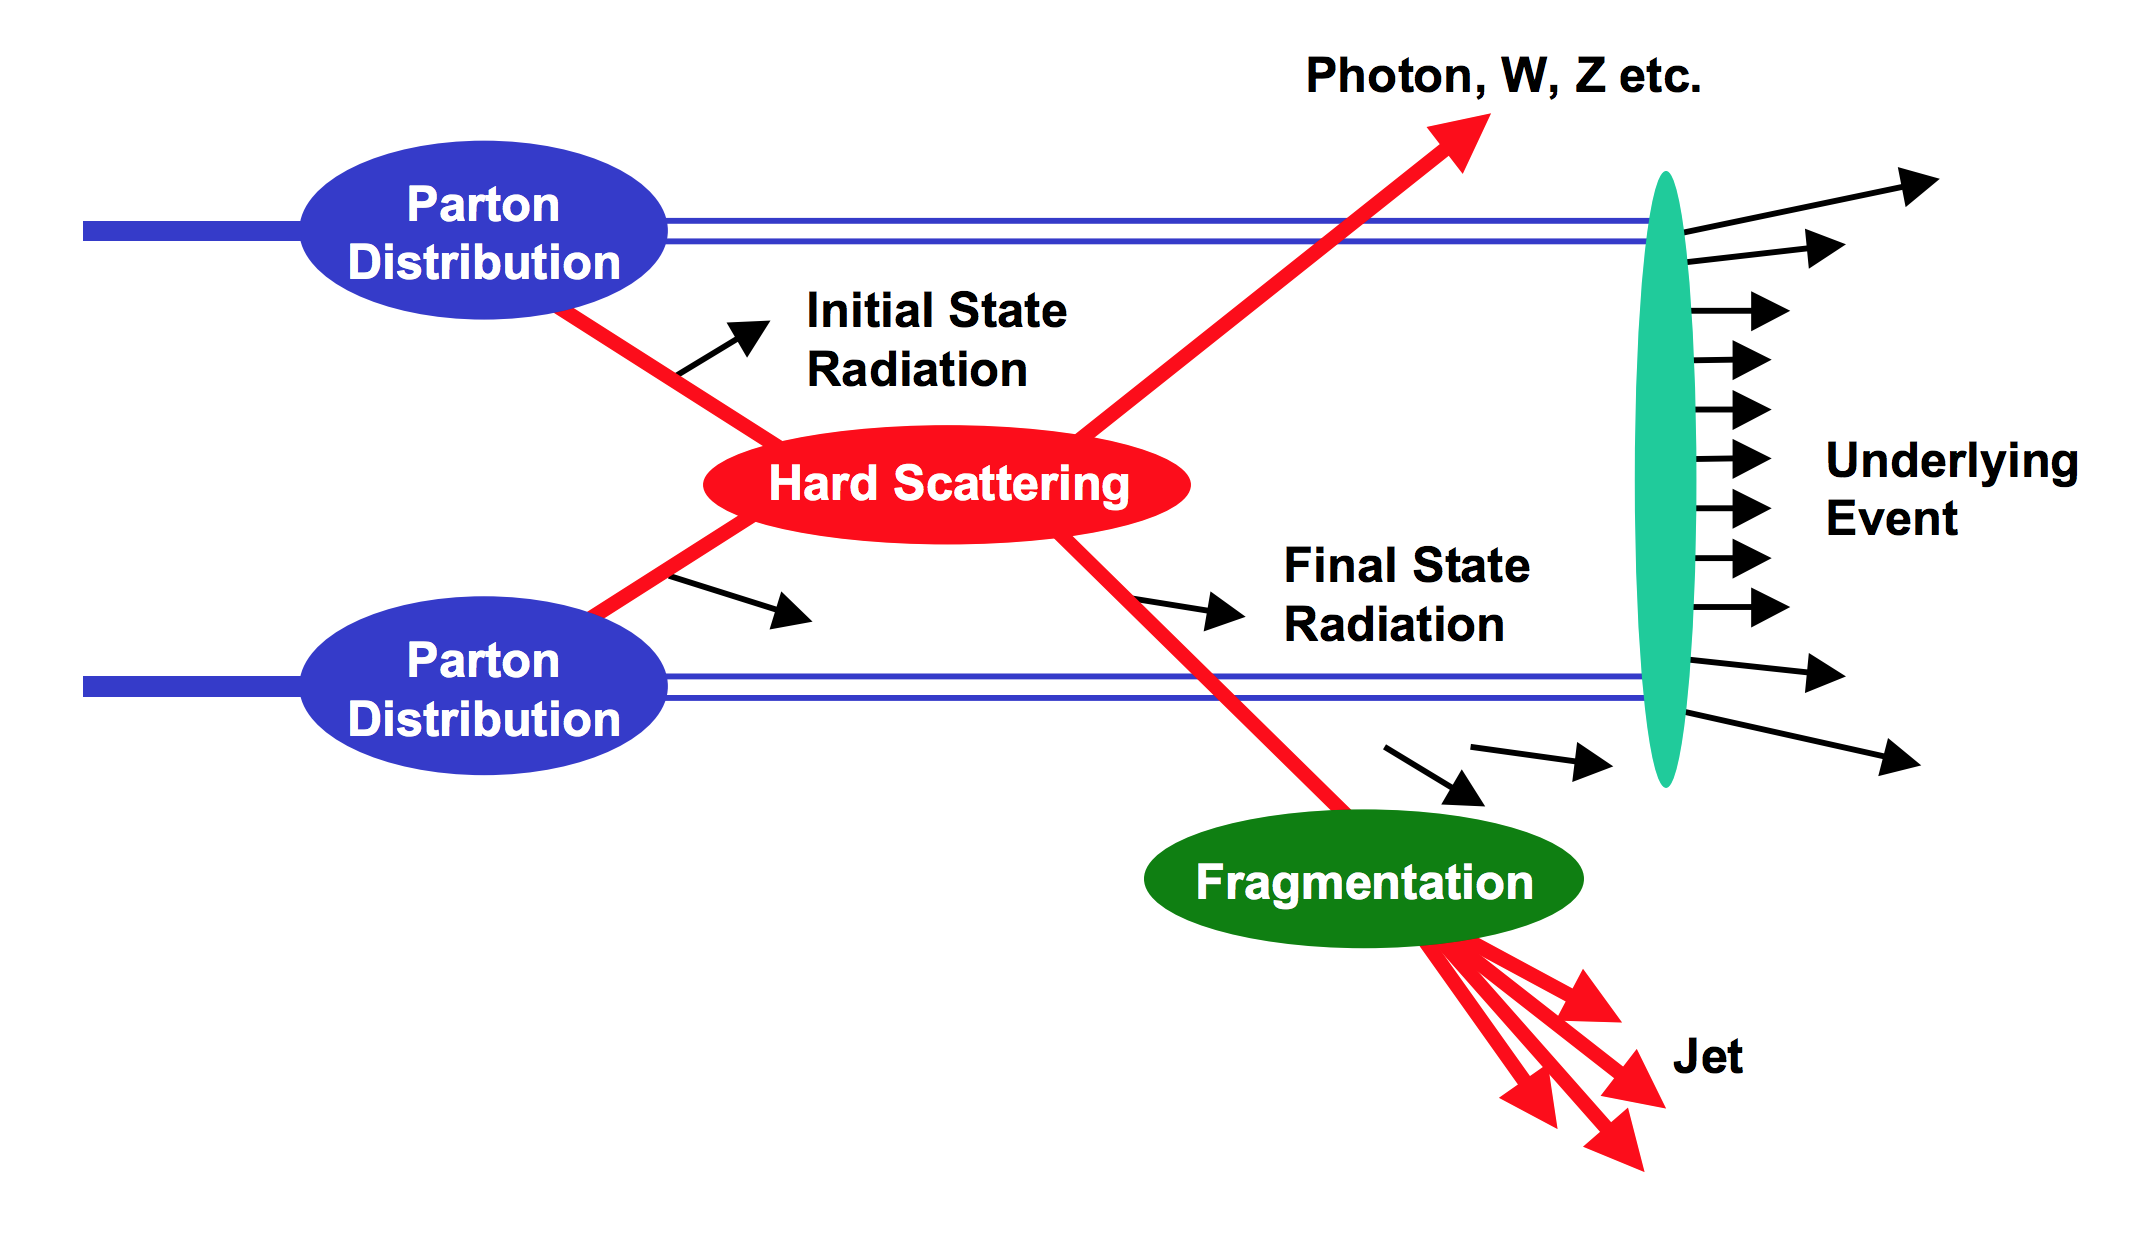
\includegraphics[width=0.7\textwidth]{figures/Theory/hh_collision.png}
  \caption{Schematic view of a hadron-hadron collision \cite{Womersley:2000cx}.}
  \label{fig:C2_had_col}
\end{figure}
and the typical features are summarized as below:
\begin{itemize}
	\item \textbf{Parton Distribution Function (PDF)} $f_{i}\left(x, Q^{2}\right)$ gives the probability of a parton with flavor $i$ (quark or gluon), carring amomentum fraction of $x$ and at the energy of Q in a proton. Parton distribution function cannot be fully calculated by perturbative QCD because of the inherent non-perturbative nature of partons. There are many different sets of PDFs that are determined by a fit to data from experimental observables in various processes. As an example, figure~\ref{fig:C2_PDF4LHC15} for \textit{PDF4LHC15} which is based on the combination of the \textit{CT14}, \textit{MMHT14} and \textit{NNPDF3.1} NNLO PDF sets \cite{Lin:2017snn}.
	\item \textbf{Fragmentation and hadronization} The processes to produce final state particles (or jets) from the partons produced in hard scattering.
	\item \textbf{Initial/Final state radiation} The incoming and outgoing partons that carry color charge can emit QCD radiation, which gives rise to additional jets. Also the charged incoming and outgoing particles can emit QED radiations with photons.
	\item \textbf{Underlying events} Products from soft processes (not come from the primary hard scattering) as the remnants of scattering interactions.
\end{itemize}
\begin{figure}[!htb]
  \centering
  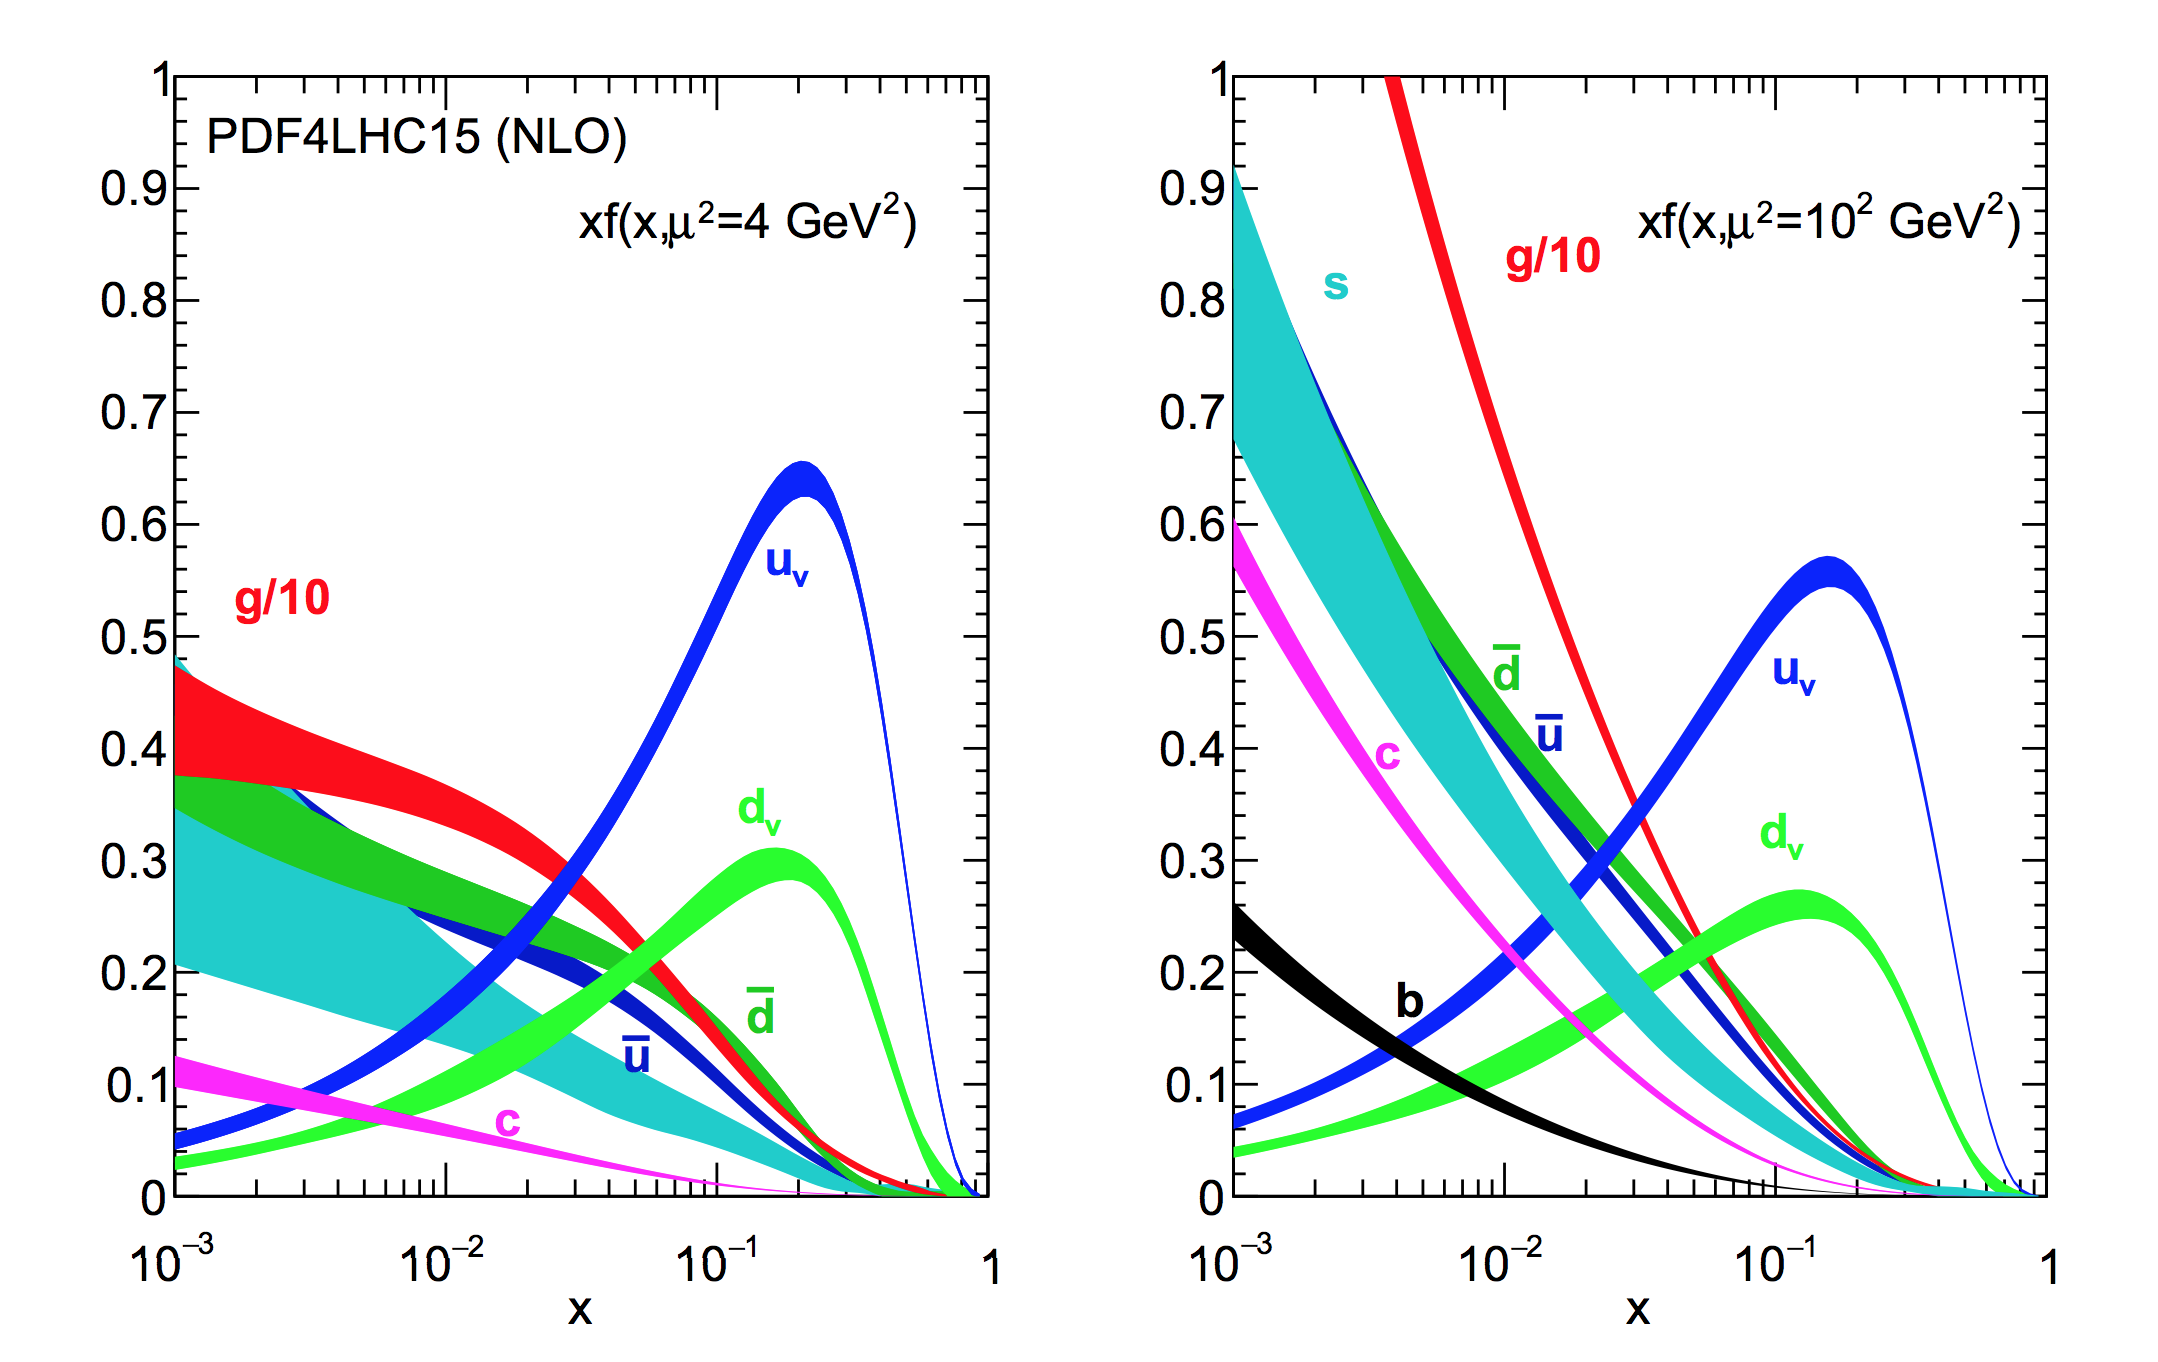
\includegraphics[width=0.7\textwidth]{figures/Theory/PDF4LHC15.png}
  \caption{The PDF4LHC15 NLO PDFs at a low scale $\mu^{2} = Q^{2} = 4 GeV^{2}$ (left) and at $\mu^{2} = Q^{2} = 100 GeV^{2}$ (right) as a function of x.}
  \label{fig:C2_PDF4LHC15}
\end{figure}

\textbf{Cross section of hard scaterring} 

According to \textit{QCD factorization theorems} \cite{Collins:1989gx}, the perturbative calculations can be applied to many important
hard processes involving hadrons. The basic problem addressed by factorization theorems is how to calculate high energy cross sections.
Conder the process of scattering between two hardons A and B to produce a final state X, the cross section $\sigma$ can be obtained 
by summing over all the subprocess cross section $\hat{\sigma}$ \cite{Stirling:1194745}
\begin{equation}
	\sigma_{AB} = \int dx_{a} dx_{b} f_{a/A}\left(x_{a}\right) f_{b/B}\left(x_{b}\right) \hat{\sigma}_{ab\rightarrow X}
\end{equation}
where $f_{q/A}\left(x_{q}\right)$ is the parton distrition functions of parton $q$.
Taking into account the leading order correction:
\begin{equation} \label{eq:xs2}
	\sigma_{AB} = \int dx_{a} dx_{b} f_{a/A}\left(x_{a}Q^{2}\right) f_{b/B}\left(x_{b}Q^{2}\right) \hat{\sigma}_{ab\rightarrow X}
\end{equation}
where $Q^{2}$ represents large momentum scale that characterizes the hard scattering.
Later on, since the finite corrections were not universal and had to be calculated separately for each process,
the perturbative $O\left(\alpha_{S}^{n}\right)$ corrections to the leading logarithm cross section in Eq.~\ref{eq:xs2}
need to be applied, one can get:
\begin{equation}
	\sigma_{AB} = \int dx_{a} dx_{b} f_{a/A}\left(x_{a}\mu_{F}^{2}\right) f_{b/B}\left(x_{b}\mu_{F}^{2}\right) \hat{\sigma}_{ab\rightarrow X}\left(\alpha_{S},\mu_{R},\mu_{F}\right)
\end{equation}
in which $\mu_{F}$ is \textit{factorization scale} which can represent the scale that separates the long- and short-distance physics,
and $\mu_{R}$ is the \textit{renormalization scale} for QCD running coupling.
$\hat{\sigma}_{ab\rightarrow X}$ is the parton-level hard scattering cross section that can be calculated perturbatively in QCD with the form of
\begin{equation} \label{eq:xs3}
	\hat{\sigma}_{ab\rightarrow X}\left(\alpha_{S},\mu_{R},\mu_{F}\right) 
		= \left(\alpha_{S}\right)^{n} \left[ \hat{\sigma}^{(0)}
		+ \left(\alpha_{S}/2\pi\right) \hat{\sigma}^{(1)}\left(\mu_{R},\mu_{F}\right)
		+ \left(\alpha_{S}/2\pi\right)^{2} \hat{\sigma}^{(2)}\left(\mu_{R},\mu_{F}\right)
		+ ... \right]
\end{equation}
where $\hat{\sigma}^{(0)}$ stands for the leading-order (LO) partonic cross section,
while $\hat{\sigma}^{(1)}$ and $\hat{\sigma}^{(2)}$ are the next-to-leading-order (NLO) and
next-to-next-to-leading-order (NNLO) cross section.

$\mu_{R}$ and $\mu_{F}$ depend on the order of truncation in Eq.~\ref{eq:xs3}.
In principle, if cross section is calculated to all orders, it is invariant under changes in these parameters.
The choices of $\mu_{R}$ and $\mu_{F}$ are arbitrary. 
To avoid unnaturally large logarithms reappearing in the perturbation series,
it is sensible to choose $\mu_{R}$ and $\mu_{F}$ values of the order of the typical momentum scales of
the hard scattering process and $\mu_{R} = \mu_{F}$ is also often assumed.
Take Drell–Yan process as an example, the standard choice is $\mu_{R} = \mu_{F} = m_{ll}$, 
where $m_{ll}$ is the invariant mass of dilepton pair.

%\subsection{Physics at hadronic collision}
\subsection{Higgs physics at LHC}
\label{higgs}

One important physics purpose of LHC is searching for Higgs boson, which was the last missing part in SM.
This section will talk about both the production and decay modes of SM Higgs boson in proton-proton collision.

%% ================================ Higgs production ===============================
\textbf{Higgs productions}

Higgs boson can be produced through several processes.
There are 4 main production modes at LHC: gluon-gluon fusion (\textit{ggF}), vector boson fusion (\textit{VBF}),
associated production with vector-bosons (also called Higgs strahlung) (\textit{VH}) 
and associated production with a pair of top/antitop quarks (\textit{ttH}) \cite{Grojean:2243593}.
Figure~\ref{fig:higgs_productions_fd} shows the corresponding Feynman diagrams of each process (at LO).
\begin{figure}[!htb]
  \centering
  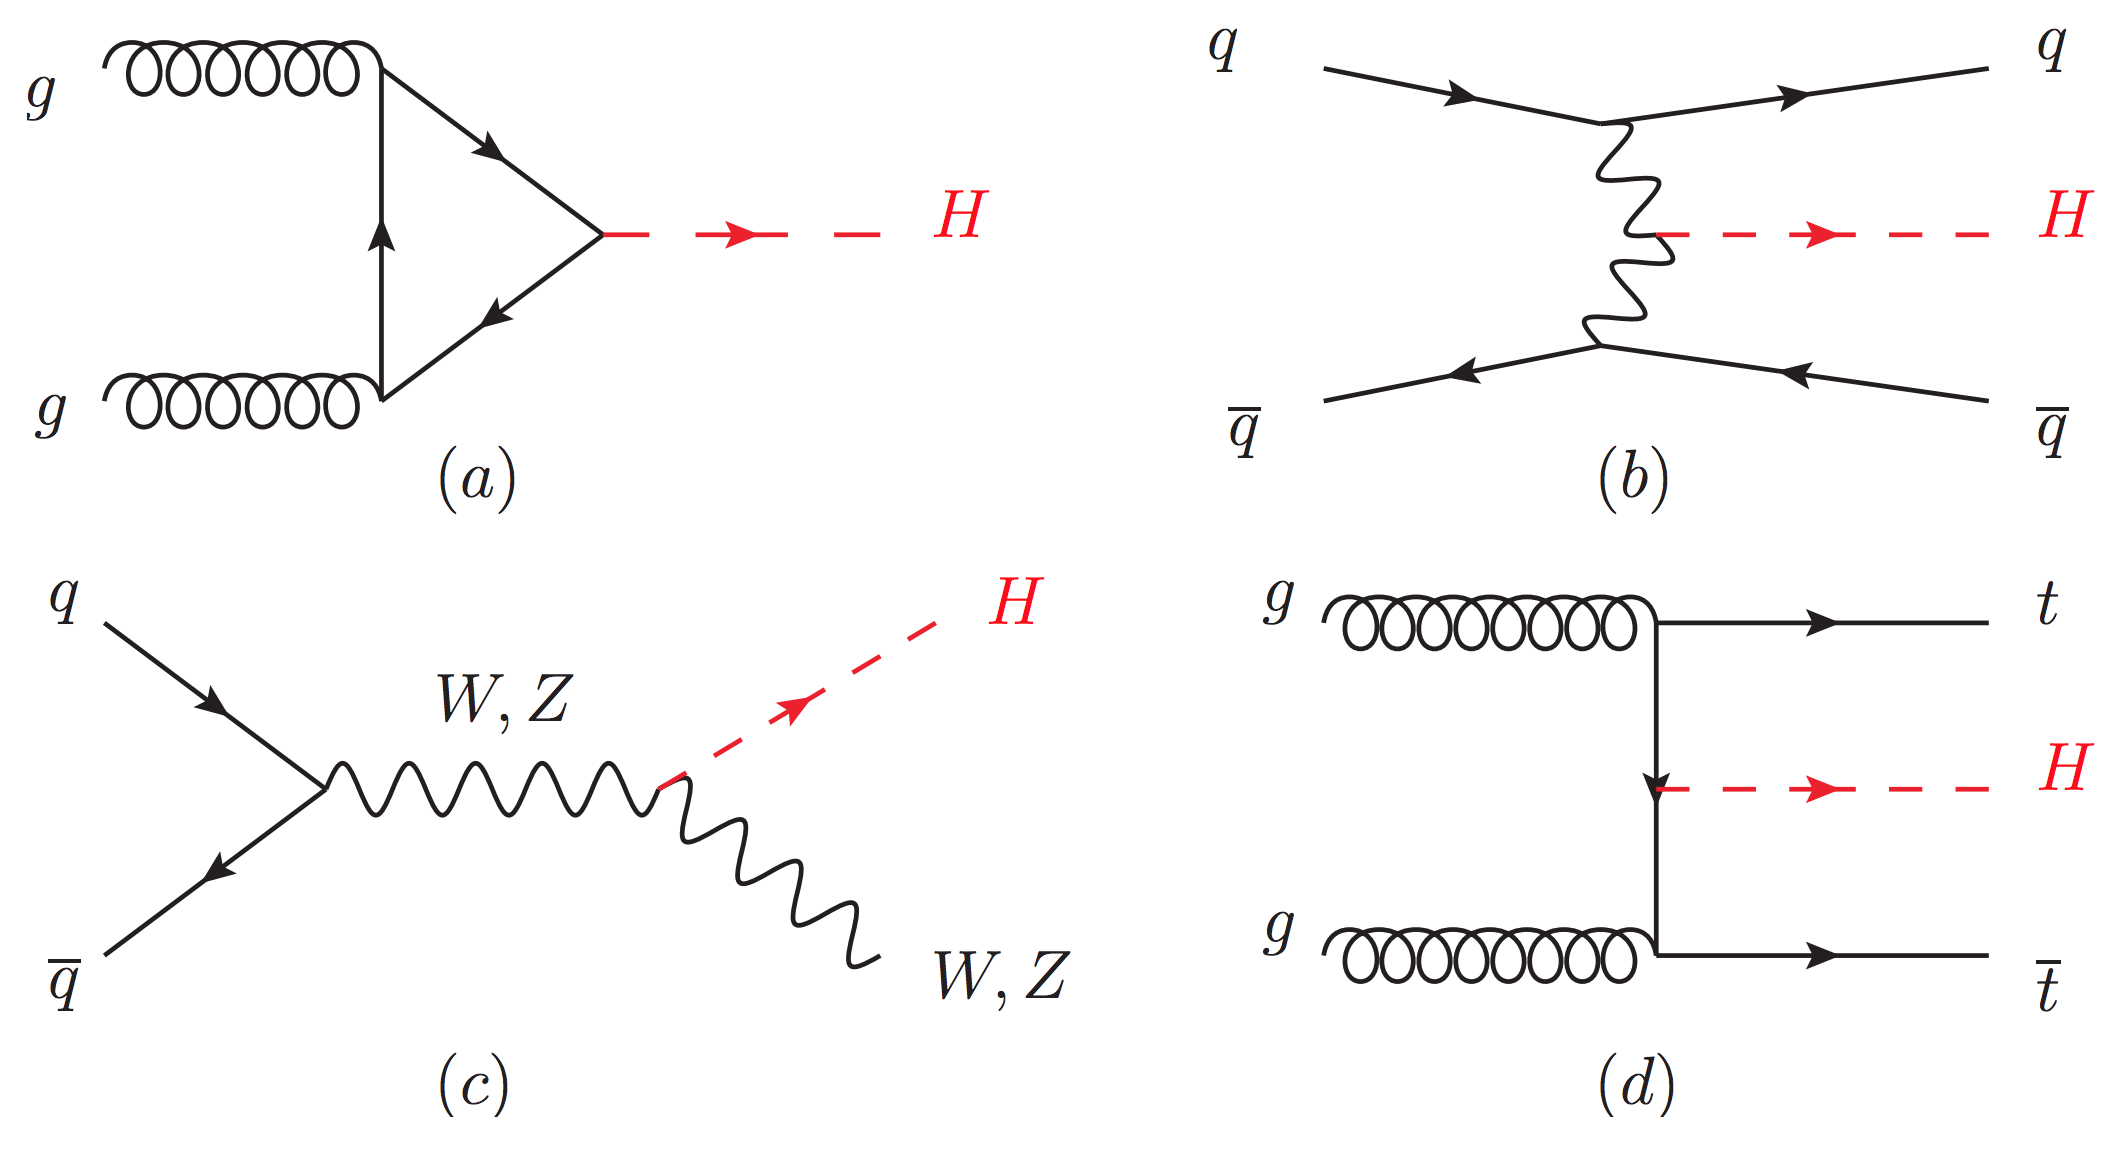
\includegraphics[width=0.8\textwidth]{figures/Theory/Figures_FeynmanHprod.png}
  \caption{Feynman diagrams of the Higgs production modes:
	   (a) ggF; (b) VBF; (c) VH; (d) ttH.}
  \label{fig:higgs_productions_fd}
\end{figure}
For pp collision, the cross section of productions of Higgs boson is as a function of center-of-mass-energy $\sqrt{s}$. 
Figure~\ref{fig:higgs_productions_xs} summarizes the cross section for SM Higgs with mass of 125 GeV.\\
\begin{figure}[!htb]
  \centering
  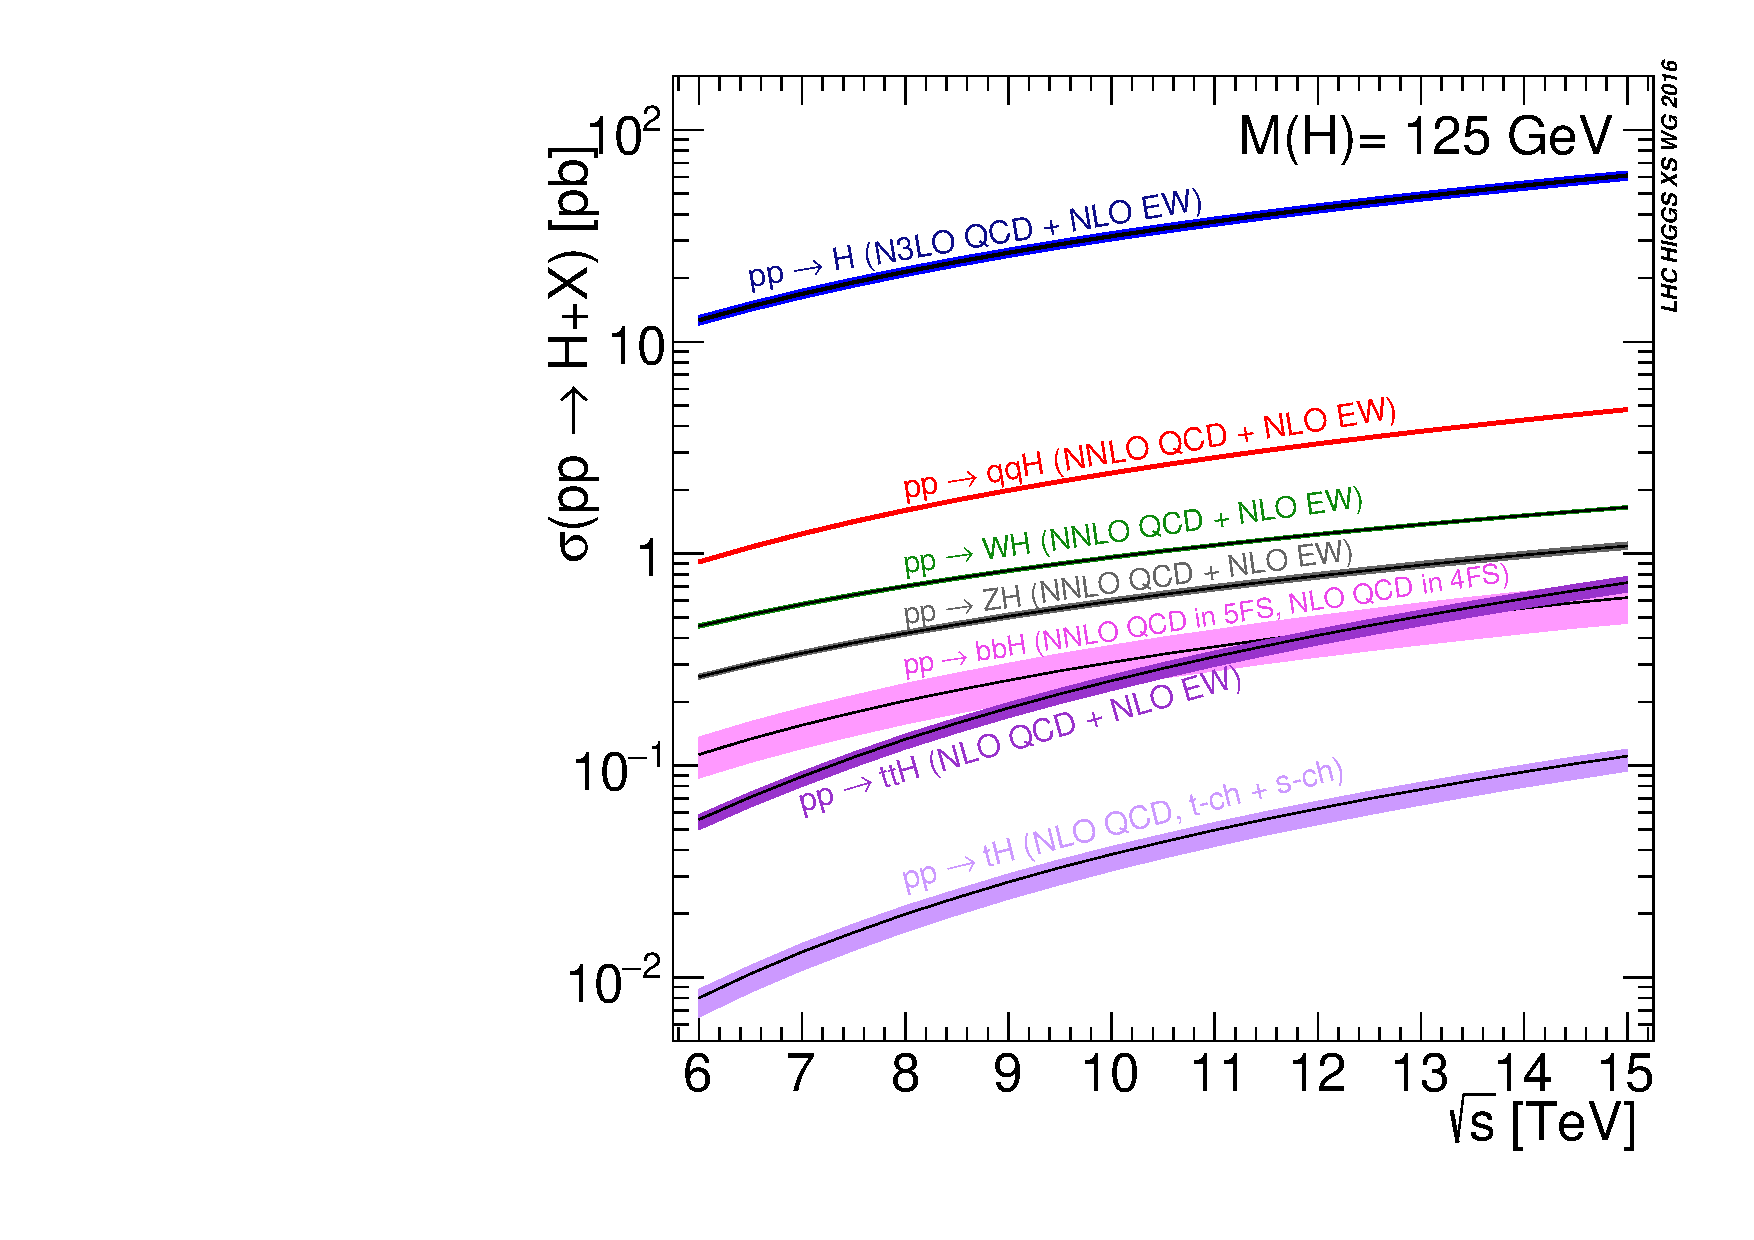
\includegraphics[width=0.5\textwidth]{figures/Theory/Plot_Escan_H125_new_sqrt.pdf}
  \caption{The SM Higgs boson production cross sections as a function of the center-of-mass-energy for pp collision.}
  \label{fig:higgs_productions_xs}
\end{figure}
Figure~\ref{fig:higgs_productions_xs2} summarizes the prospect of different Higgs boson production cross sections 
as a function of Higgs mass for pp collision center-of-mass-energy at 13 TeV and 14 TeV \cite{deFlorian:2227475}. 
\begin{figure}[!htb]
  \centering
  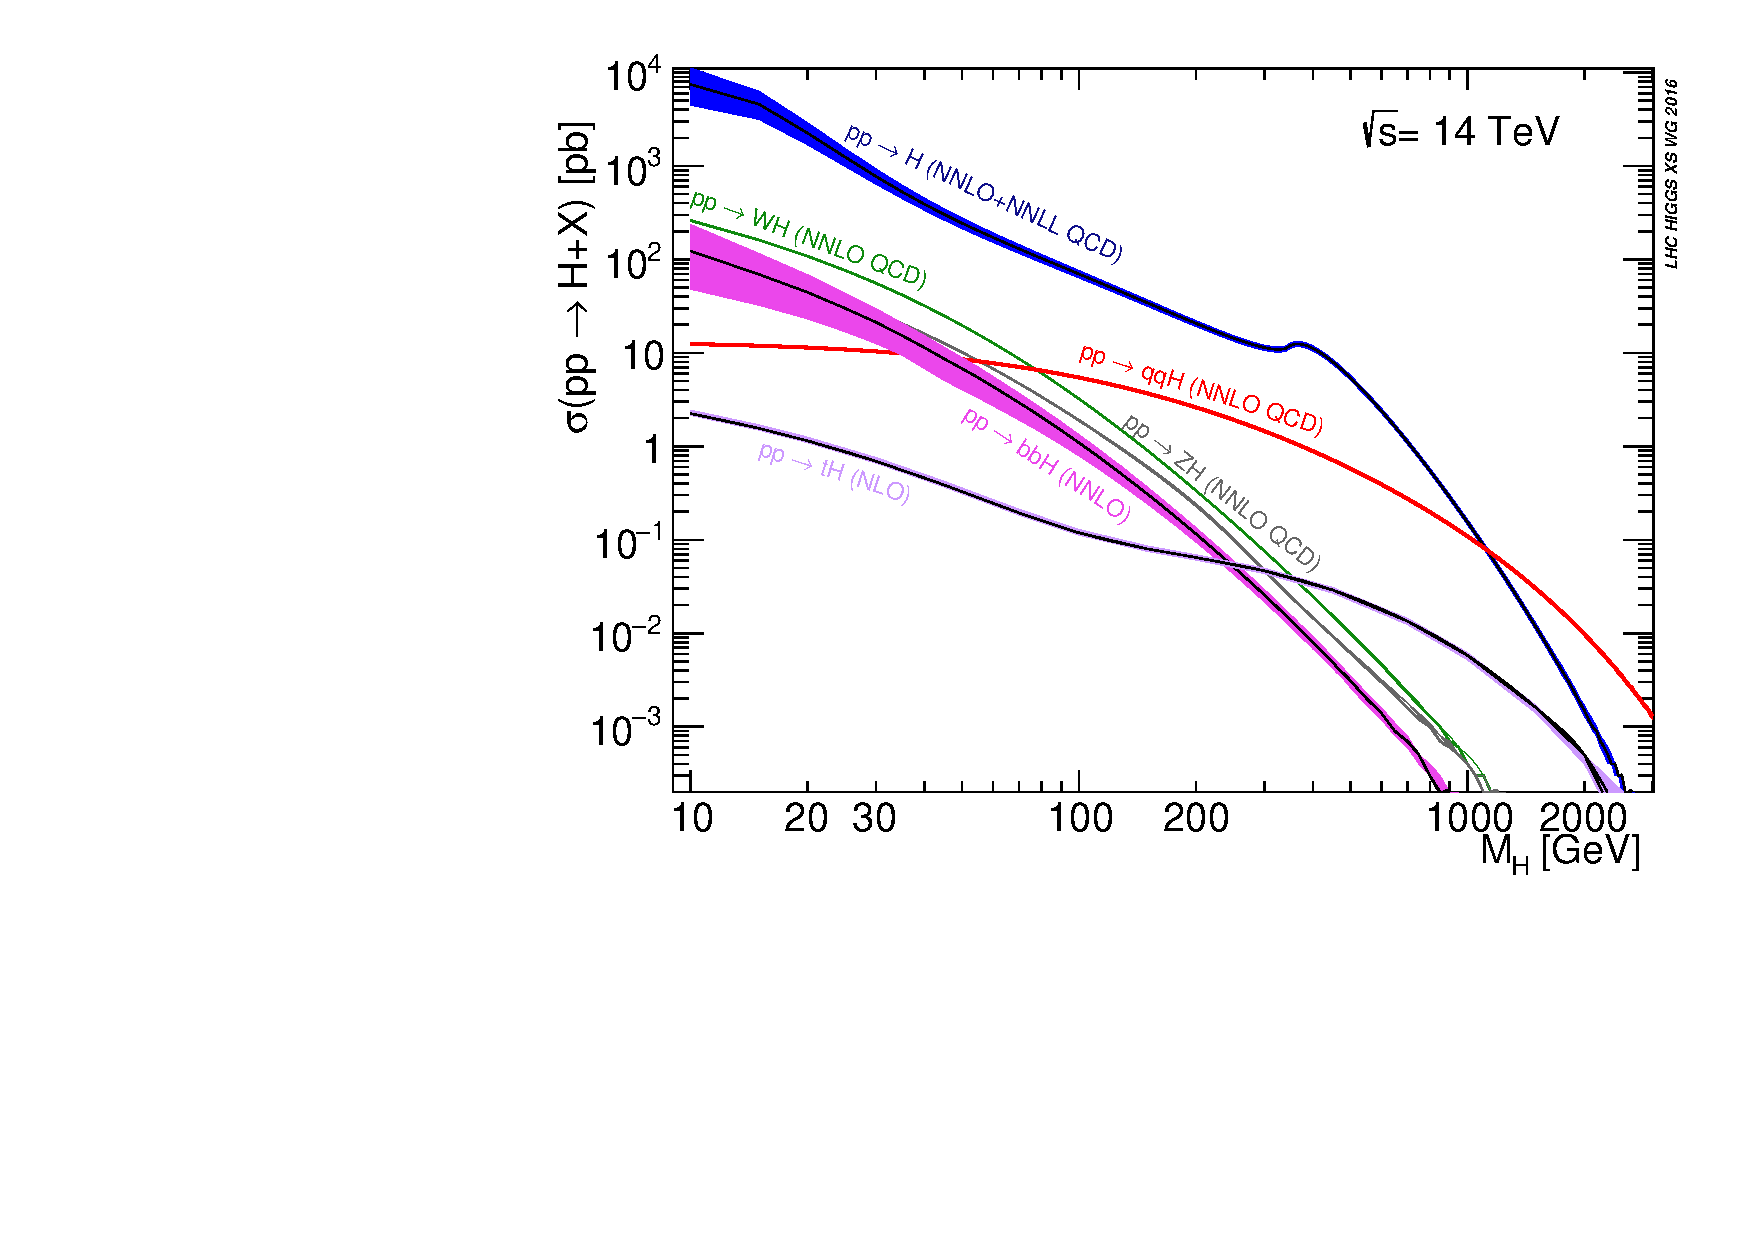
\includegraphics[width=0.45\textwidth]{figures/Theory/plotAll_14tev_BSM_sqrt.pdf}
  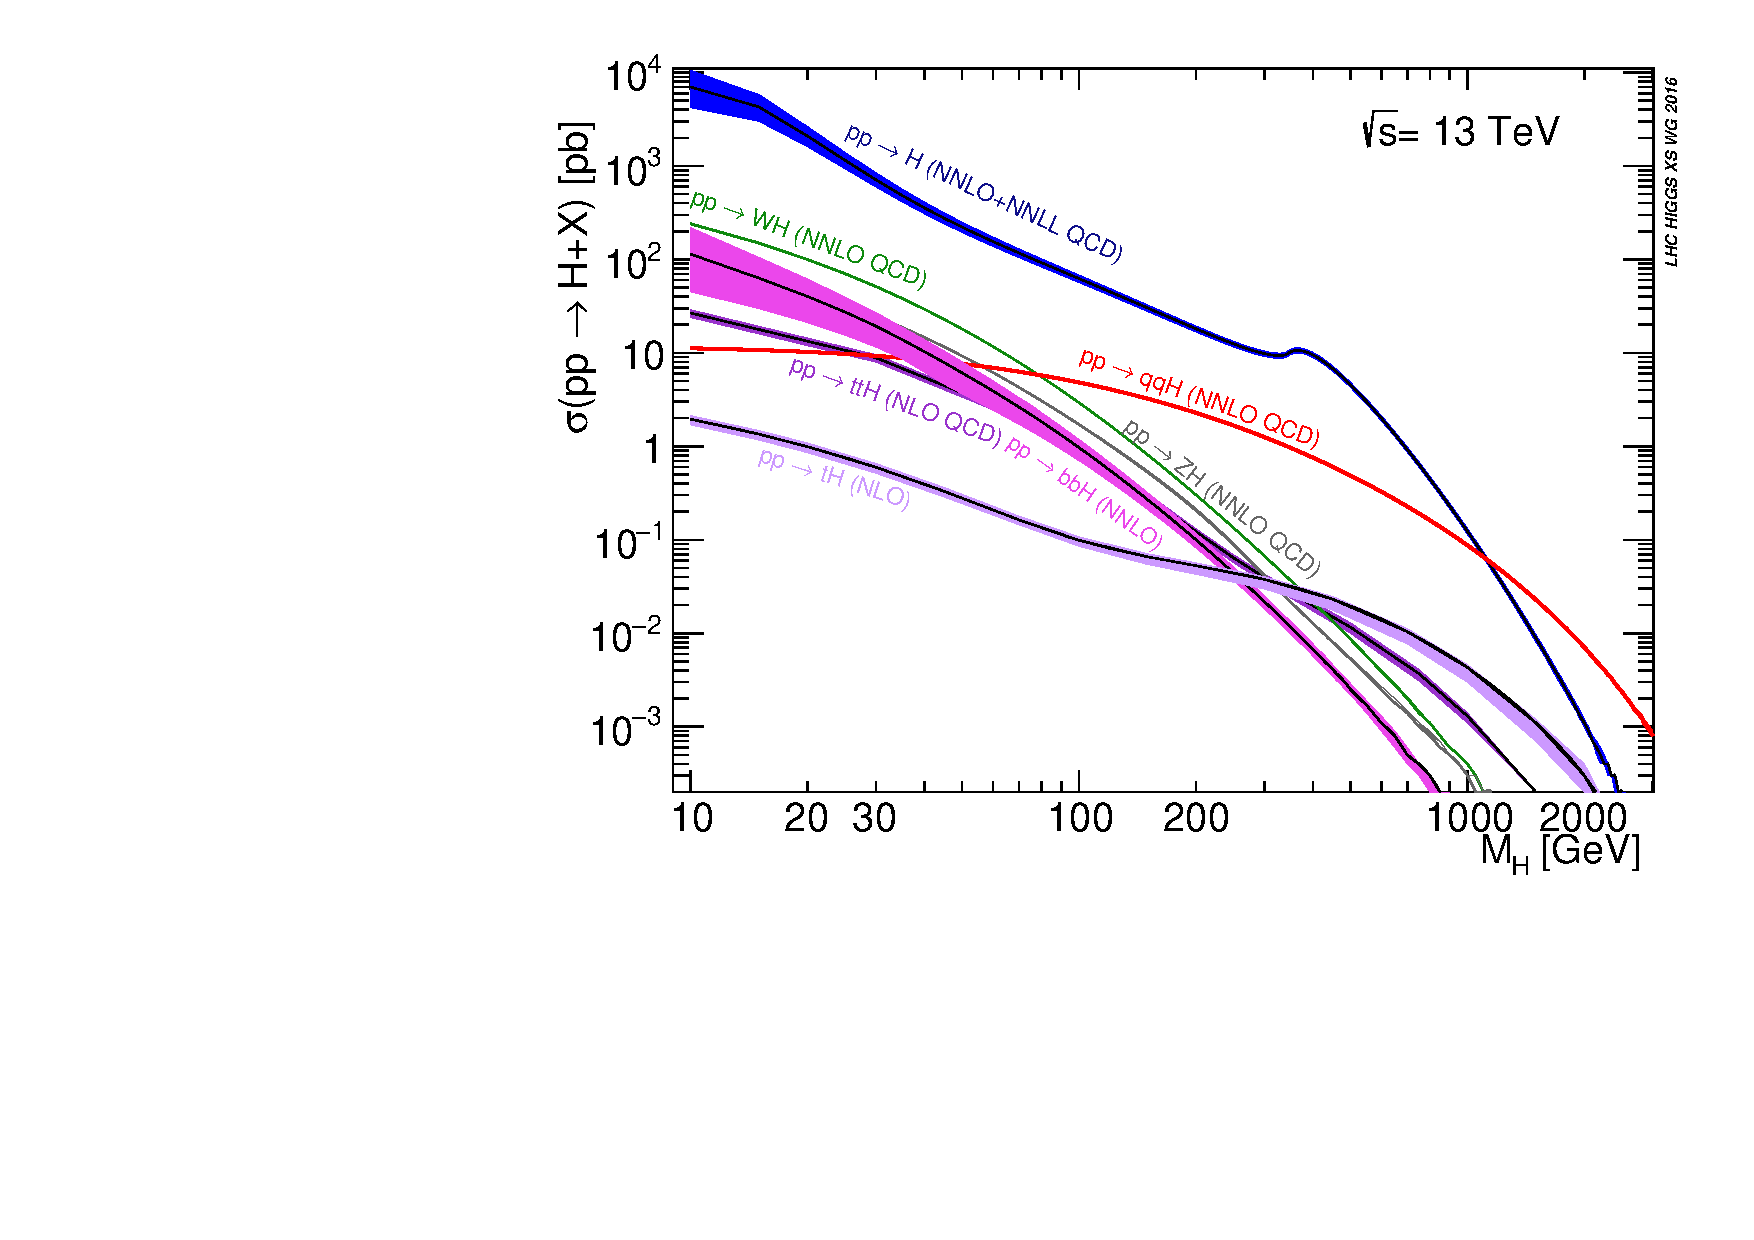
\includegraphics[width=0.45\textwidth]{figures/Theory/plotAll_13tev_BSM_sqrt.pdf}
  \caption{Higgs boson production cross section for various production modes as a function of the Higgs mass mH for $\sqrt{s}$ = 13 TeV (left) and 14 TeV (right) for pp collision.}
  \label{fig:higgs_productions_xs2}
\end{figure}

%% ================================ Higgs decays ===================================
\textbf{Higgs decays}

Higgs boson can interact with gauge bosons and fermions through gauge coupling and Yukawa coupling as introduced in section~\ref{symbreaking}.
Figure~\ref{fig:higgs_decay_fd} depicts Feynman diagrams of possible Higgs decay channels.
\begin{figure}[!htb]
  \centering
  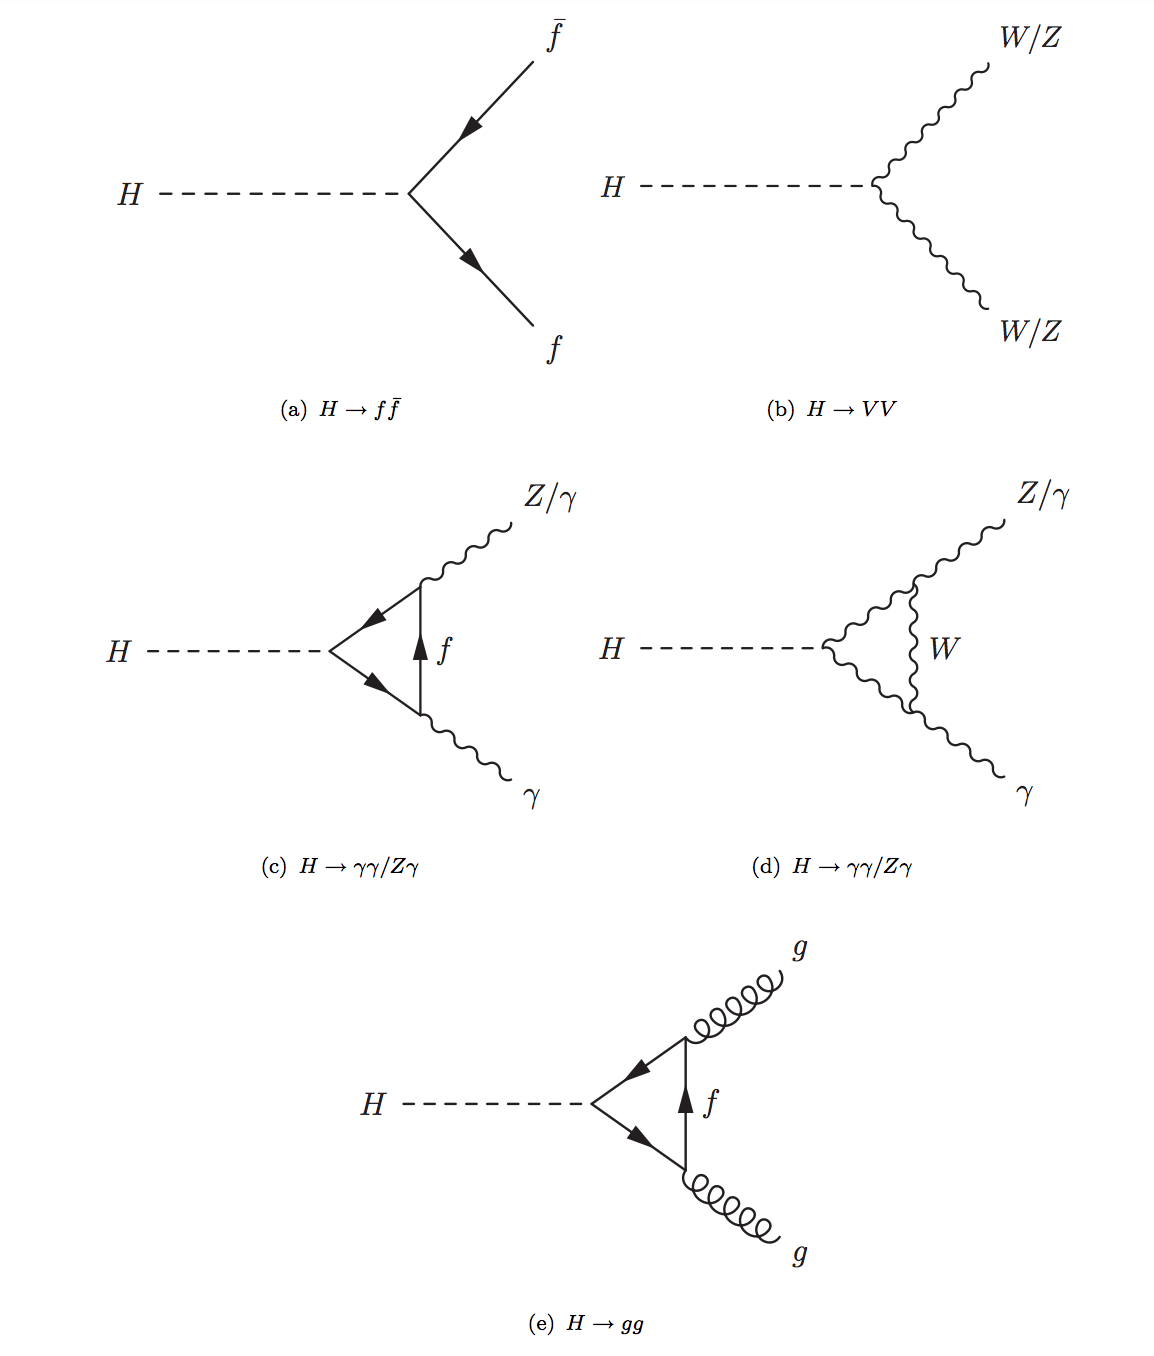
\includegraphics[width=0.8\textwidth]{figures/Theory/Figures_Feynman_Hdecay.png}
  \caption{SM Higgs decay channels.}
  \label{fig:higgs_decay_fd}
\end{figure}
The branching ratio of Higgs boson decaying into different final states as a function of Higgs mass is shown in figure~\ref{fig:higgs_decay_br}.
\begin{figure}[!htb]
  \centering
  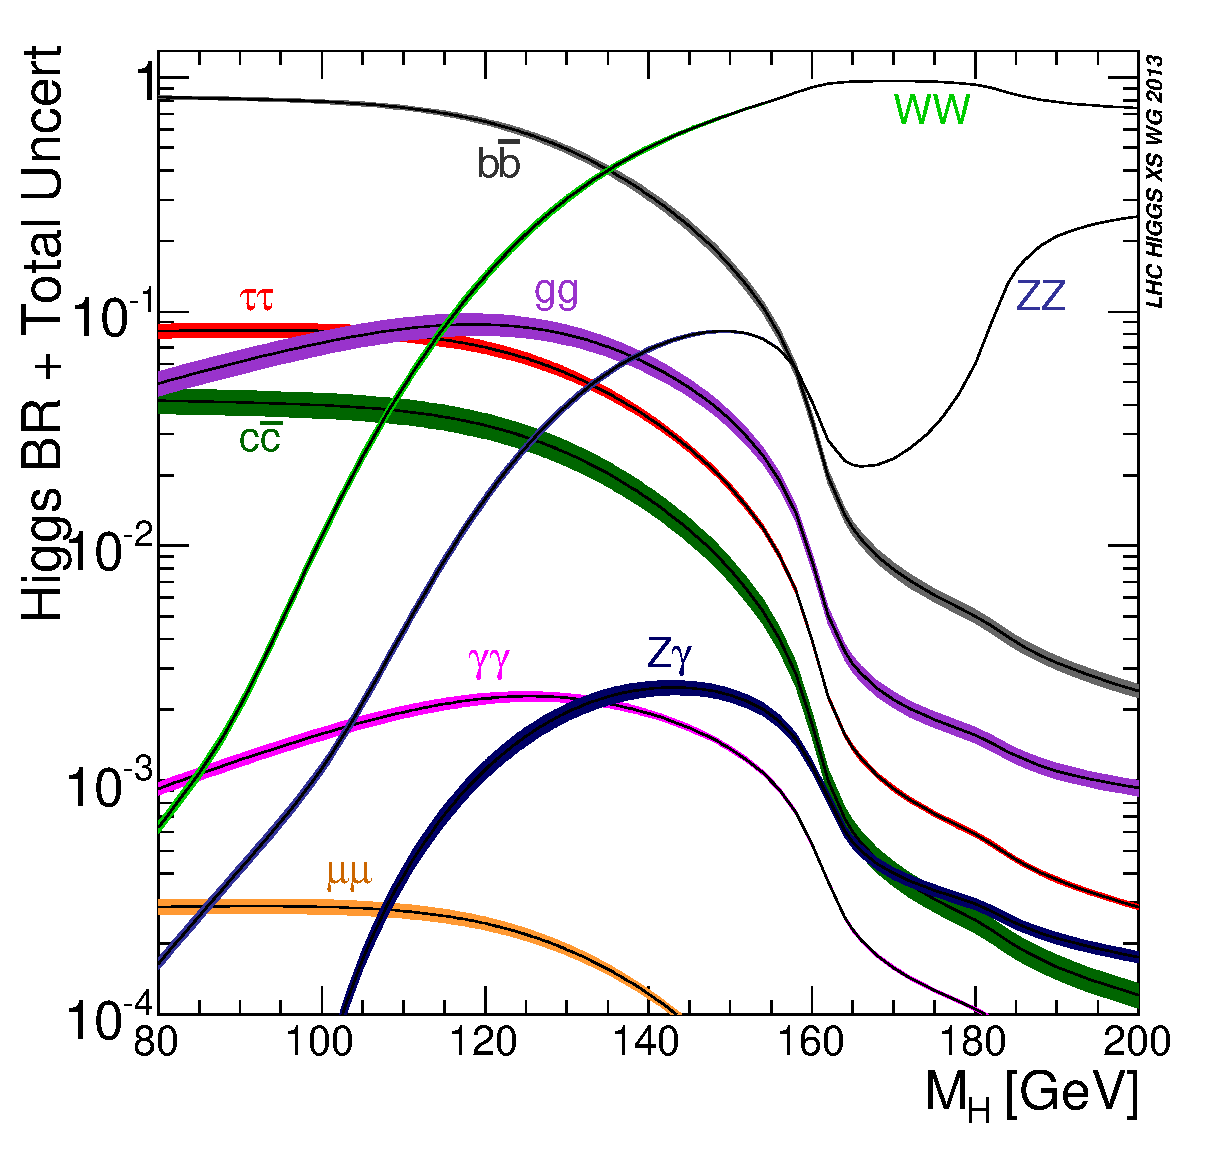
\includegraphics[width=0.5\textwidth]{figures/Theory/Higgs_BR_LM.eps}
  \caption{Branching ratio of Higgs decays \cite{Heinemeyer:1559921}. }
  \label{fig:higgs_decay_br}
\end{figure} 

%% ====================================== High mass related ===========================
(\textbf{BSM Higgs models})



%\subsection{Higgs Physics at LHC}
\subsection{Diboson physics}
\label{diboson}

The study of diboson physics is another important test for SM of particle physics in electroweak sector, 
in which vector boson scattering is a key process for probing the mechanism of electroweak symmetry breaking (EWSB).
In the meantime, the non-resonant diboson productions are crucial backgrounds for Higgs study at LHC, which make the precise measurement of their cross section becomes very important.

%% ====================================== Diboson productions ========================
\textbf{Diboson productions}

About $90\%$ of diboson productions at hadron collider is from quark-antiquark annihilation,
while others are contributed from gluon initiated process.
Figure~\ref{fig:diboson_fd1} shows the tree-level Feynman diagrams of diboson production.
\begin{figure}[!htb]
  \centering
  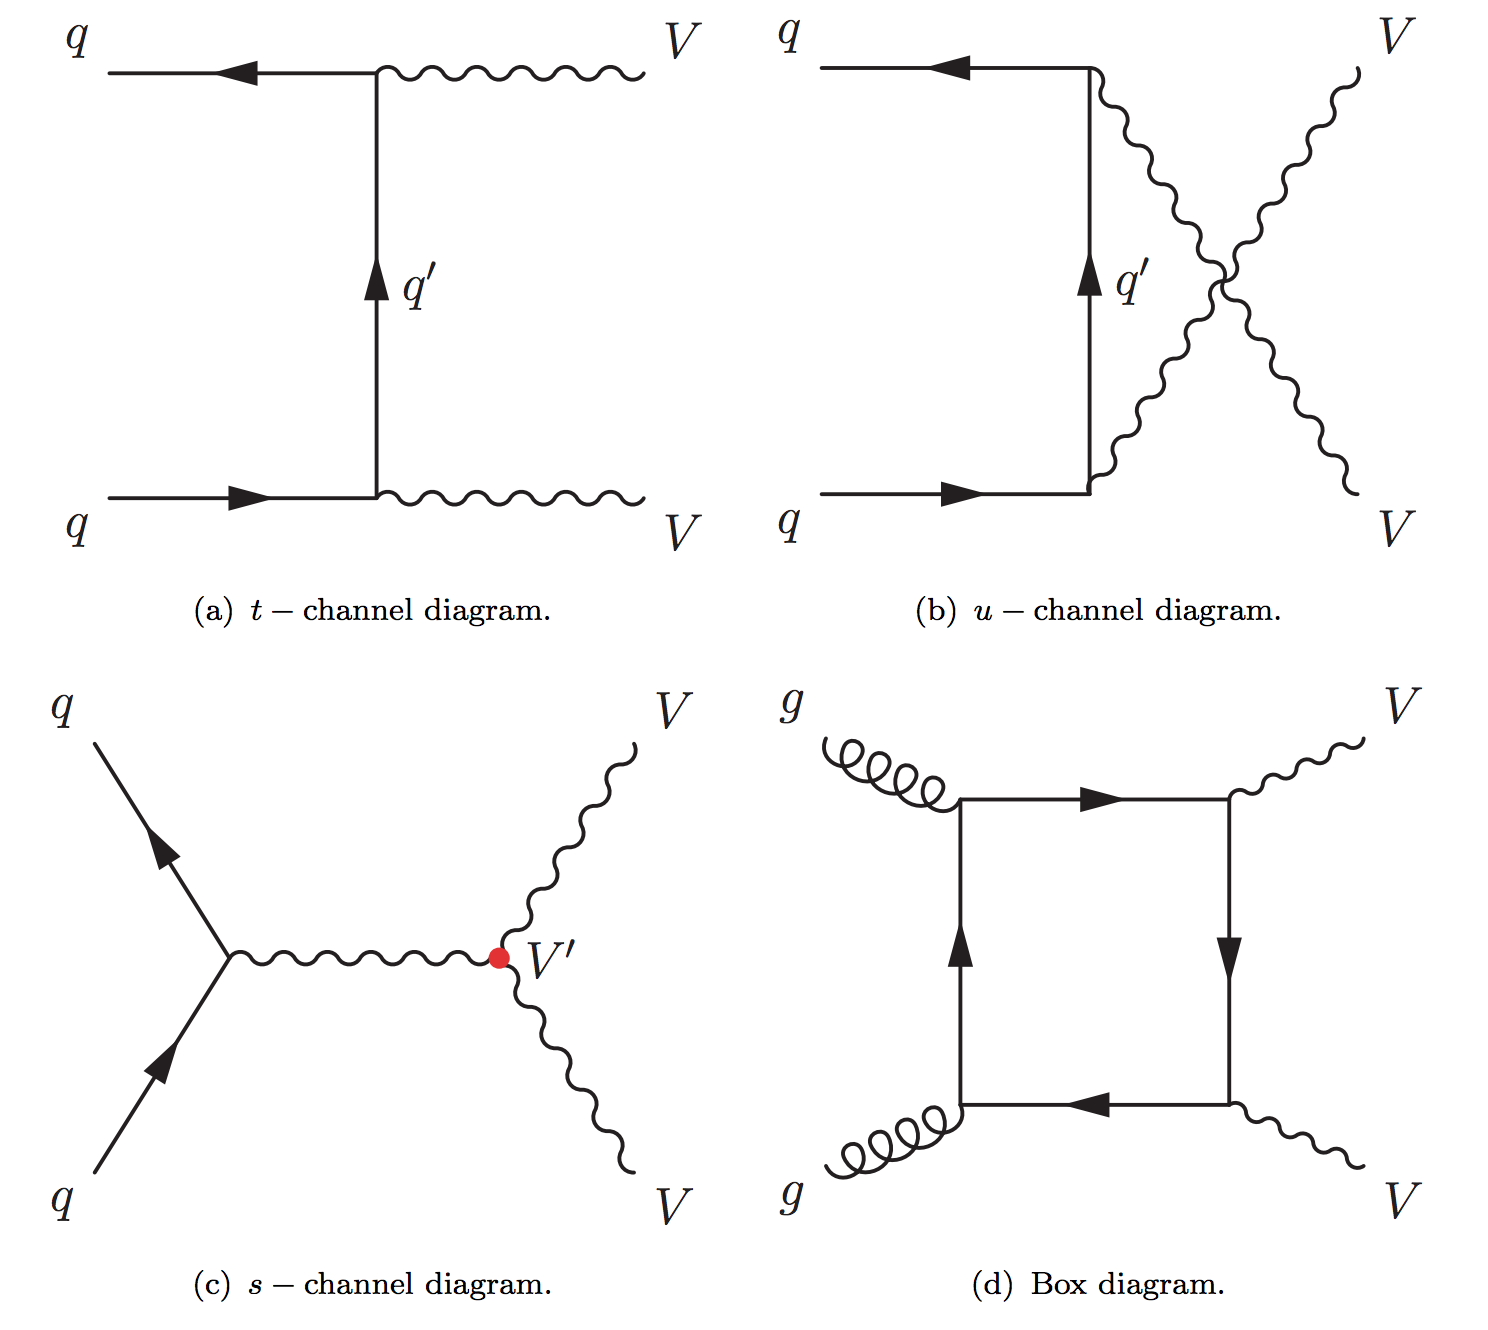
\includegraphics[width=0.7\textwidth]{figures/Theory/diboson_prod_fey.png}
  \caption{The tree-level Feynman diagrams of diboson production at LHC.}
  \label{fig:diboson_fd1}
\end{figure}
Then figure~\ref{fig:diboson_xs1} illuminates the total production cross-section presented by ATLAS
as a function of centre-of-mass energy $\sqrt{s}$ from 7 to 13 TeV for several diboson processes comparing 
to some other major processes in hardon collision.
The cross section for diboson processes are measured at NNLO. 
\begin{figure}[!htb]
  \centering
  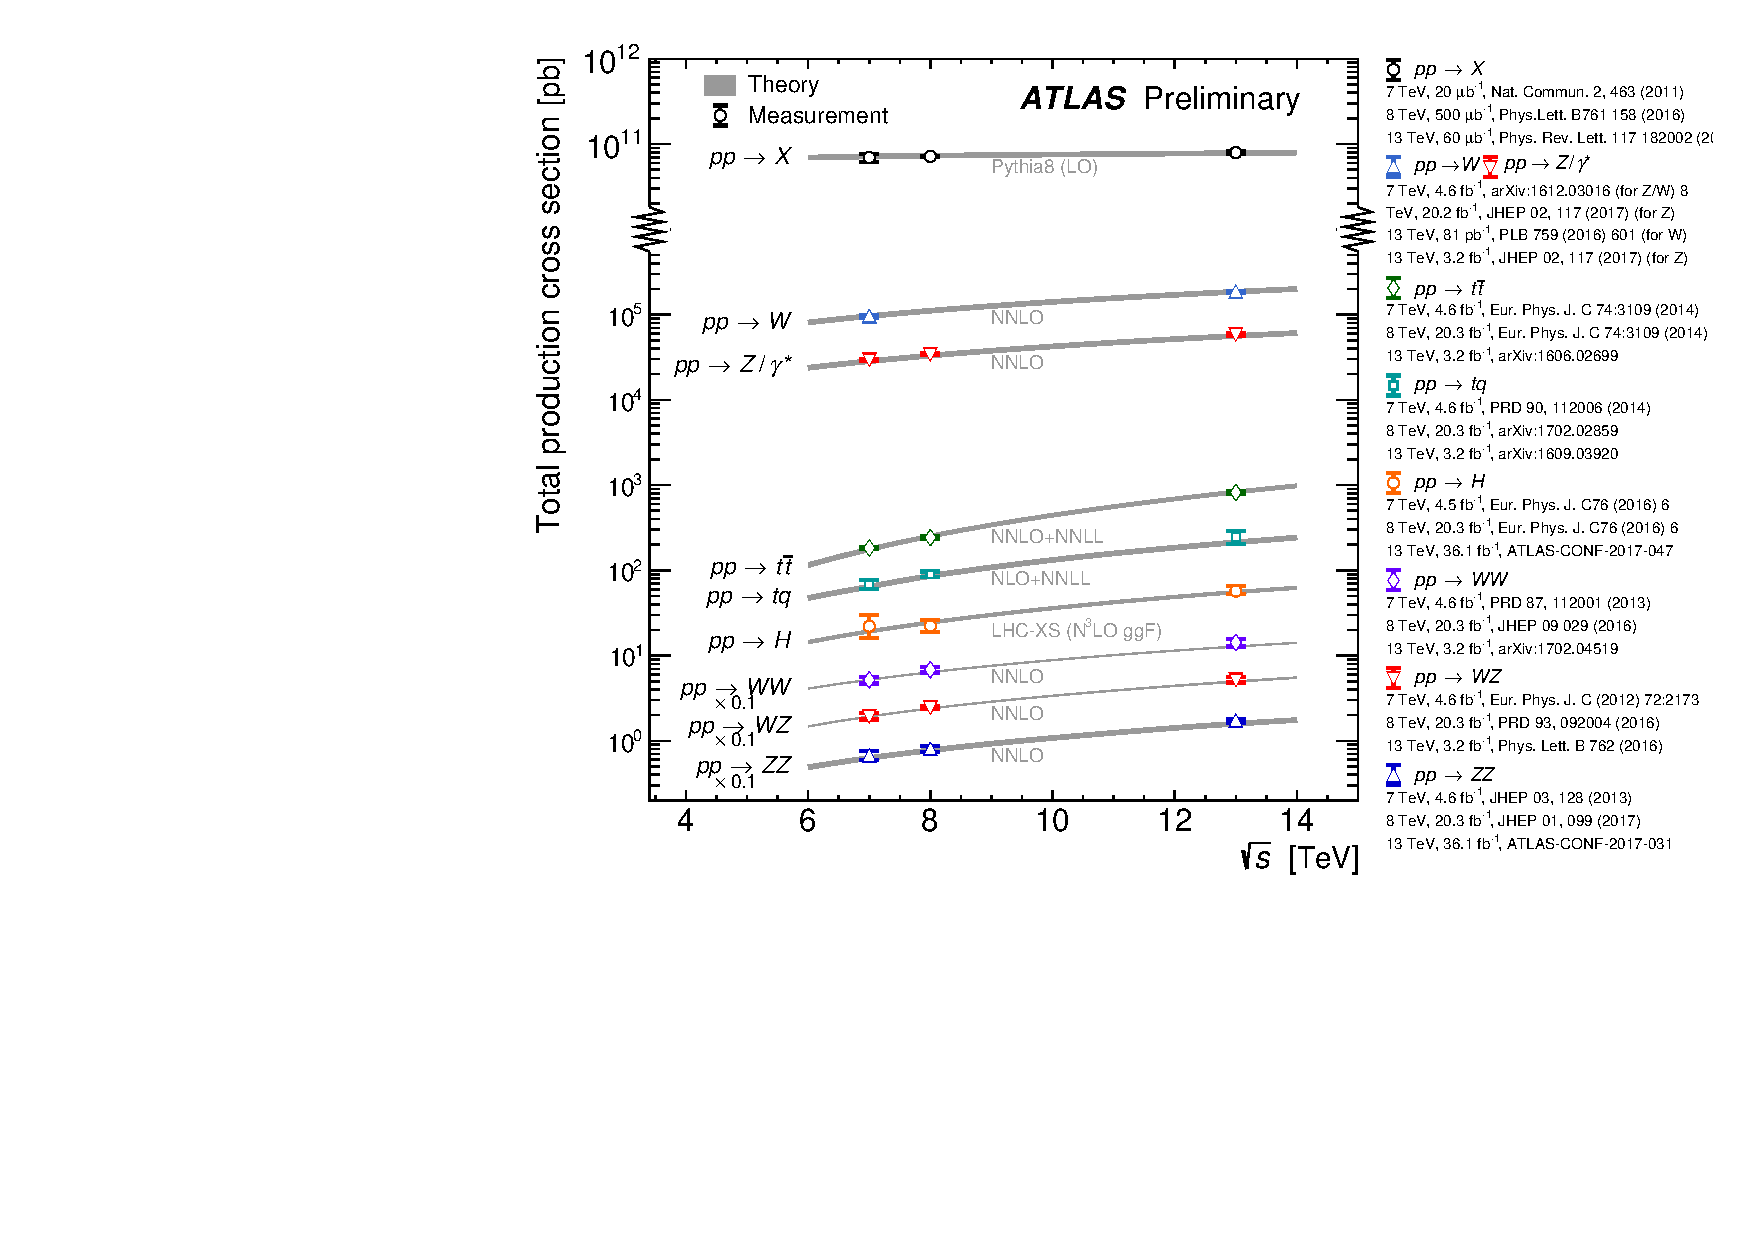
\includegraphics[width=0.7\textwidth]{figures/Theory/ATLAS_n_SMSummary_SqrtS.pdf}
  \caption{Total production cross-section presented by ATLAS as a function of centre-of-mass energy $\sqrt{s}$ from 7 to 13 TeV for some selected processes,
	   the diboson measurements are scaled by a factor 0.1 to allow a presentation without overlaps.}
  \label{fig:diboson_xs1}
\end{figure}

%% ======================================= Vector boson scattering ===================
\textbf{Vector boson scattering}

The $SU(2)_{L} \times U(1)_{Y}$ structure in SM predicts self-interactions between electroweak gauge bosons.
Those self-couplings can involve either three or four gauge bosons at a single vertex, known as triple gauge coupling (\textit{TGC}) and
quartic gauge couplings (\textit{QGC}), repectively.
Vector boson scattering or fusion (\textit{VBS} or \textit{VBF}) is carried out 
by four electroweak vector bosons, namely $Z$, $W^{\pm}$ and photon $(\gamma)$ as the Feynman diagrams shown in figure~\ref{fig:vbs_fd1}. 
And the vertexes include either those self-interactions
or the interactions with Higgs boson described in figure~\ref{fig:vbs_fd2}.
\begin{figure}[!htb]
  \centering
  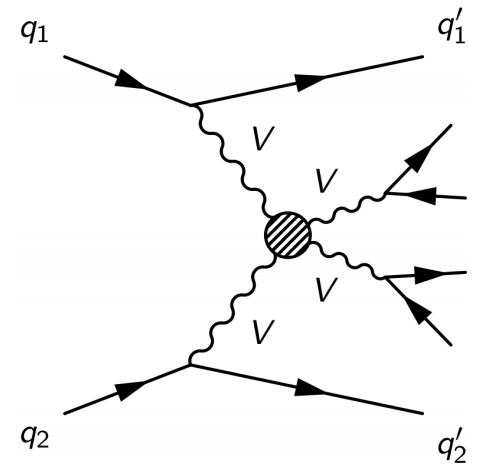
\includegraphics[width=0.4\textwidth]{figures/Theory/VBS.png} 
  \caption{Feynman disgrams of vector boson scattering.}
  \label{fig:vbs_fd1}
\end{figure}
\begin{figure}[!htb]
  \centering
  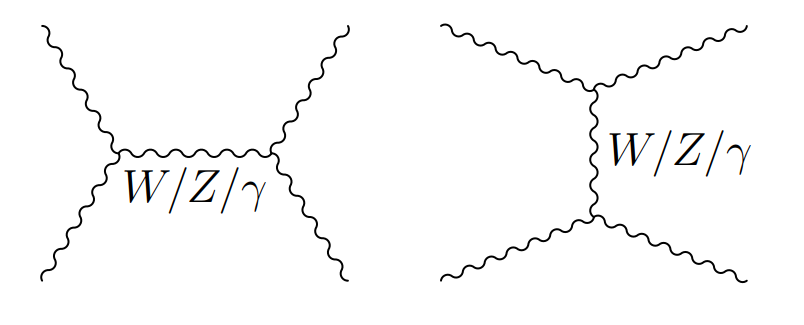
\includegraphics[width=0.6\textwidth]{figures/Theory/vbs_tgc.png} \\
  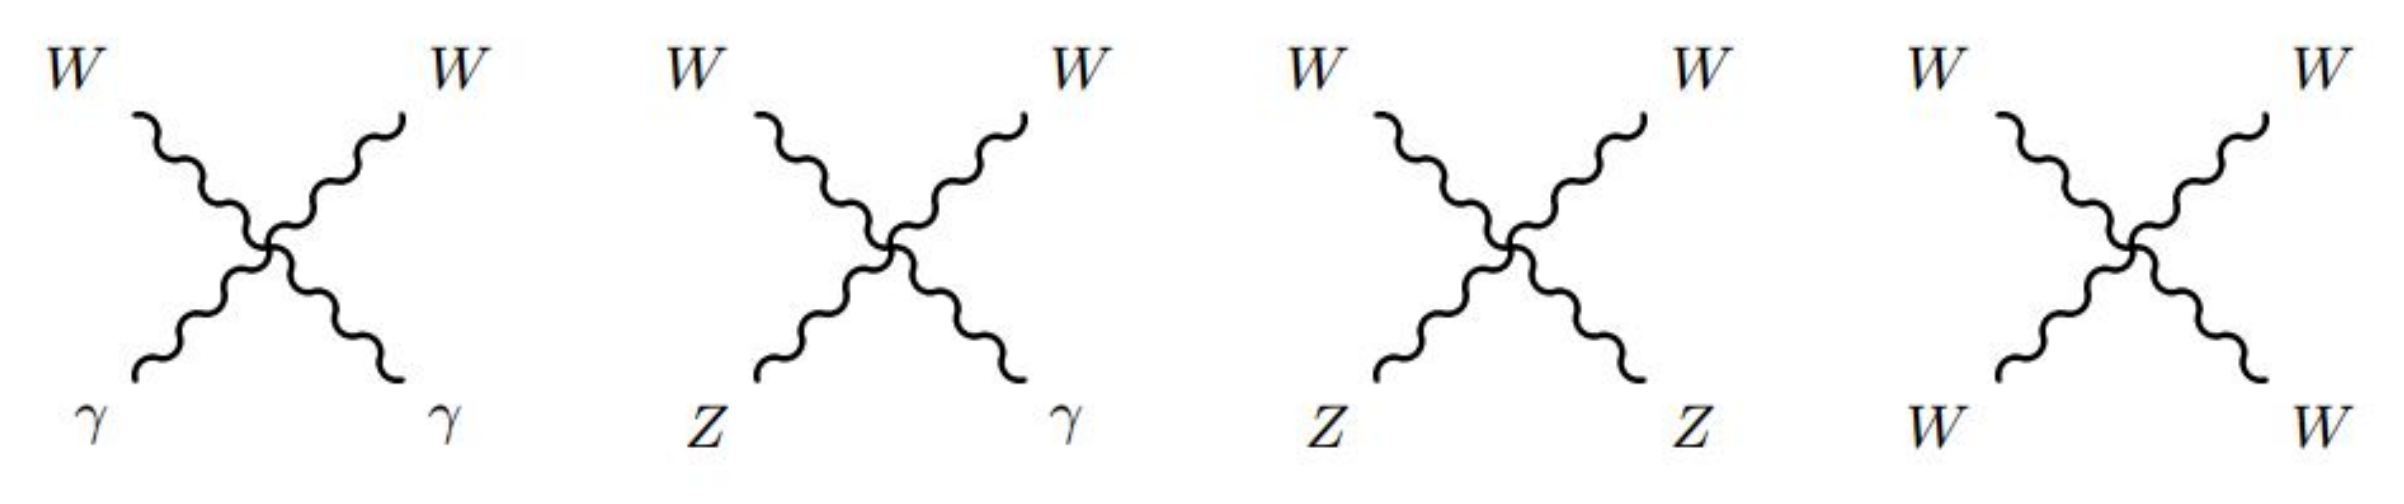
\includegraphics[width=1.0\textwidth]{figures/Theory/vbs_qgc.png} \\
  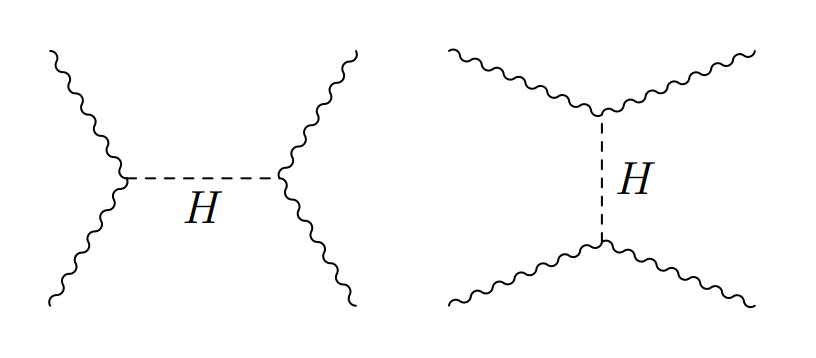
\includegraphics[width=0.6\textwidth]{figures/Theory/vbs_higgs.png} 
  %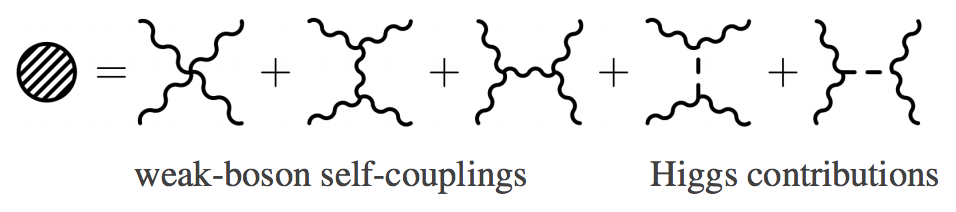
\includegraphics[width=1.0\textwidth]{figures/Theory/VBS_vertex.png}
  \caption{Feynman disgrams of vertexes involving QGC, TGC and Higgs.}
  \label{fig:vbs_fd2}
\end{figure}

The amplitudes of leading-order (LO) VBS can be expressed as:
\begin{equation} \label{eq:amp_tgc}
\begin{split}
	& {iM}_{TGC}^{s-channel} = -i\frac{g_{1}^{2}}{4m_{W}^{4}}[s(t-u)-3m_{W}^{2}(t-u)] \\
	& {iM}_{TGC}^{t-channel} = -i\frac{g_{1}^{2}}{4m_{W}^{4}}\left[t(s-u)-3m_{W}^{2}(s-u)+\frac{8m_{W}^{2}}{s}u^{2}\right]
\end{split}
\end{equation}
\begin{equation}
	{iM}_{QGC} = i\frac{g_{1}^{2}}{4m_{W}^{4}}\left[s^{2}+4st+t^{2}-4m_{W}^{2}(s+t)-\frac{8m_{W}^{2}}{s}ut\right]
\end{equation}
\begin{equation} \label{eq:amp_higgs}
\begin{split}
	{iM}_{Higgs} & = -i\frac{C_{\nu}^{2}g_{1}^{2}}{4m_{W}^{2}}\left[\frac{(s-2m_{W}^{2})^{2}}{s-m_{H}^{2}} + \frac{(t-2m_{W}^{2})^{2}}{t-m_{H}^{2}}\right] \\
                     & \simeq -i\frac{C_{\nu}^{2}g_{1}^{2}}{4m_{W}^{2}}(s+t)
\end{split}
\end{equation}
Combined s- and t-channel of TGC in Eq.~\ref{eq:amp_tgc}:
\begin{equation}
	{iM}_{TGC} = -i\frac{g_{1}^{2}}{4m_{W}^{4}}\left[s^{2}+4st+t^{2}+3m_{W}^{2}t-5m_{W}^{2}s+8m_{W}^{2}\frac{t^{2}}{s}\right]
\end{equation}
Then by combining the QGC term, the amplitude of self-couplings can be written as:
\begin{equation} \label{eq:self_coup}
	{iM}_{TGC} + {iM}_{QGC}= i\frac{g_{1}^{2}}{4m_{W}^{2}}(s+t) + {O}((s/m_{W}^{2})^{0})
\end{equation}
In Eq.~\ref{eq:self_coup}, the amplitude grows as a function of center-of-mass energy ($\sqrt{s}$),
which violates the unitarity in the TeV region.
Considering the Higgs term in Eq.~\ref{eq:amp_higgs} perfectly cancels out this growing,
and the remaining term ${O}((s/m_{W}^{2})^{0})$ depends on the total amplitude in SM.

In conclusion, Higgs boson acts as “moderator” to unitarize high-energy longitudinal vector boson scattering
by restoring unitarity of total amplitude in high energy region.

%\subsection{Diboson physics}

\chapter{The Large Hadron Collider and the ATLAS Detector}

\section{The Large Hadron Collider}
Located near the French-Swiss border at the European Organization for Nuclear Research (CERN),
the Large Hadron Collider (LHC) is the world’s largest and most powerful particle collider.
It's the proton-proton collider with center-of-mass energy up to 14 TeV.
The beams inside the LHC are made to collide at four locations around its 27-kilometer accelerator ring, 
corresponding to the positions of four particle detectors – ATLAS, CMS, ALICE and LHCb.
With its unprecedented energy, the LHC is designed to observe physics that involve highly massive particles
which have never been observable in earlier lower energy accelerators.

\subsection{Operation history and machine layout}

%% ================================= history ==============================
\textbf{Operation history}

The LHC \cite{Bruning:2004ej, Buning:2004wk, Benedikt:2004wm, Evans_2008} 
is a two-ring-superconducting-hadron accelerator and collider lies in a tunnel 27 kilometres in circumference and as deep as 175 metres underground.
It's designed to provide proton-proton (pp) collisions at the centre-of-mass energy ($\sqrt{s}$) up to 14~\tev
with a unprecedented luminosity of $10^{34} cm^{-2} s^{-1}$.
In the meantime, it can also collide heavy (Pb) ions with an energy of 2.8~\tev~ per nucleon and a peak luminosity of $10^{27} cm^{-2} s^{-1}$.
Table~\ref{tab:LHC_parameters} shows the main design parameters of the LHC for proton-proton collisions.
\begin{table}[htbp]
  \centering
  \caption{Summary of design parameters of the LHC for pp collisions.}
  \label{tab:LHC_parameters}
  \begin{tabular}{cc}
    \hline
    Circumference	& 26.7 km\\
    Beam energy at collision	& 7 ~\tev\\
    Beam energy at injection	& 0.45~\tev \\
    Dipole field at 7~\tev	& 8.33 T \\
    Luminosity		& $10^{34} cm^{-2} s^{-1}$ \\
    Beam current	& 0.56 A \\
    Protons per bunch	& $1.1 \times 10^{11}$ \\
    Number of bunches	& 2808 \\
    Nominal bunch spacing	& 24.95 ns \\
    Normalized emittance	& 3.75 $\mu$m \\
    Total crossing angle	& 300 $\mu$rad \\
    Energy loss per turn	& 6.7 keV \\
    Critical synchrotron energy	& 44.1 eV \\
    Radiated power per beam	& 3.8 kW \\
    Stored energy per beam	& 350 MJ \\
    Stored energy in magnets	& 11 GJ \\
    Operating temperature	& 1.9 K \\
    \hline
  \end{tabular}
\end{table}

The LHC was built from 1998 to 2008. 
It started its first beam in September 2008, but then was interrupted by a quench incident only after a few days running.
Then it resumed the operation in November 2009 with a low energy beams.
From March 2010, physics runs took place at the centre-of-mass energy of 7~\tev.
Later on, this energy was increased in 2012 to $\sqrt{s} = 8~\tev$, with an integrated luminosity of 20.3~\ifb, and this period is called "run-1".
After run-1, the LHC was shut down for two years for hardware maintenance and upgrade, starting from February 2013.

The second operation period with higher centre-of-mass energy at 13~\tev~ started from 2015 called "run-2".
And it continued to the end of 2018 with total integrated luminosity reaching about 147 $fb^{-1}$ for ATLAS.
Figure~\ref{fig:lumi_vs_month} shows the cumulative luminosity as a function of time in month delivered to ATLAS experiment during stable beams 
in years from 2011 to 2018.
\begin{figure}[!htb]
  \centering
  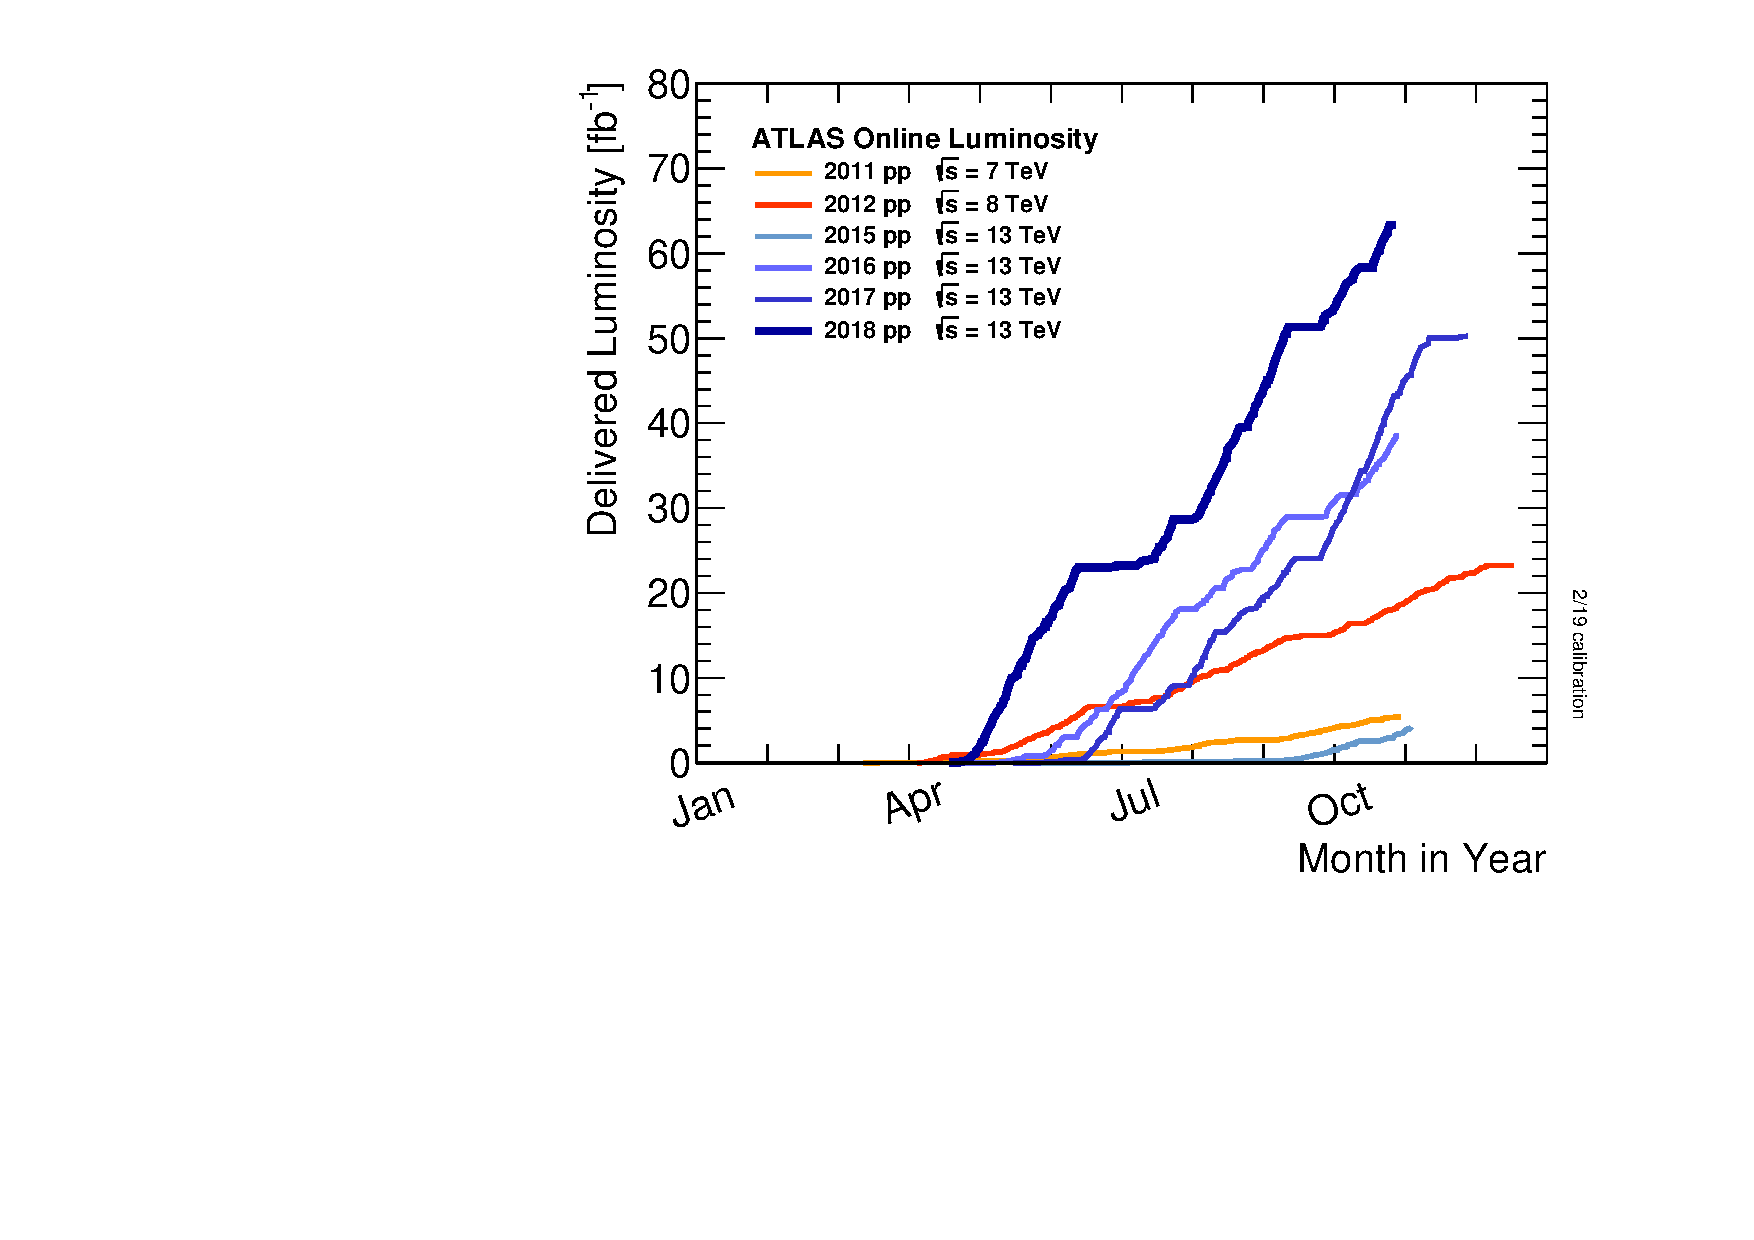
\includegraphics[width=0.6\textwidth]{figures/Detector/intlumivsyear.pdf}
  \caption{Cumulative luminosity as a function of time in years from 2011 to 2018 for ATLAS detector.}
  \label{fig:lumi_vs_month}
\end{figure}

%% ======================================= layout ==============================
\textbf{Machine layout}

The layout of CERN accelerator complex is shown in figure~\ref{cern_layout}.
The protons are accelerated by a series of machines before being injected into the main cavity.
At beginning, the 50~\mev~ protons are produced in the linear particle accelerator LINAC2, 
and then further accelerated to 1.4~\gev~ in Proton Synchrotron Booster (PSB).
The protons are then injected into the Proton Synchrotron (PS) to gain the energy of 26~\gev~ and further accelerated to 450~\gev~ in Super Proton Synchrotron (SPS).
At the end, they are injected into the main ring, and can reach a maximum energy of 7~\tev.

\begin{figure}[!htb]
  \centering
  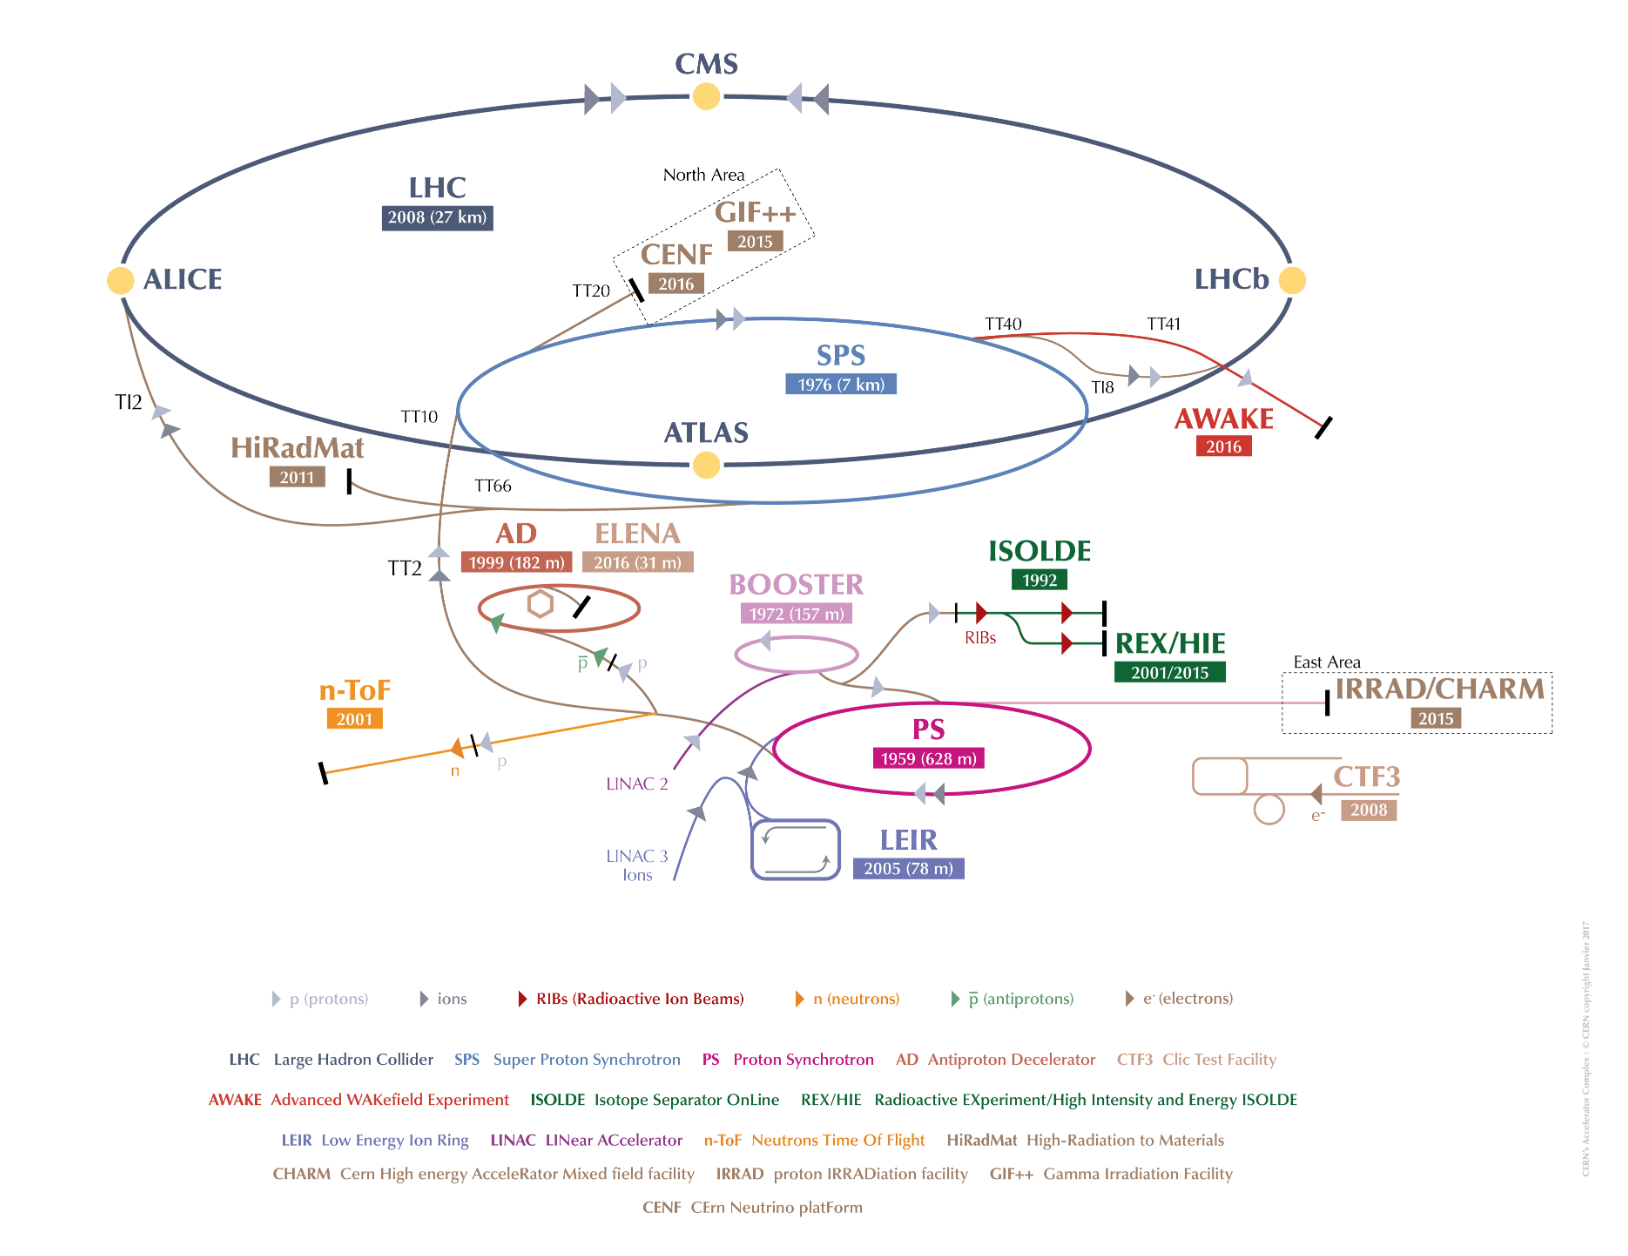
\includegraphics[width=1.0\textwidth]{figures/Detector/LHC_v2017.png}
  \caption{CERN accelerator complex \cite{Mobs:2197559}.}
  \label{cern_layout}
\end{figure}

The collisions can occur in 4 points, with corresponding 4 major detector experiments that are briefly described as follows:
\begin{itemize}
	\item \textbf{ATLAS}: A Toroidal LHC ApparatuS, one of the two general-purpose particle detector experiments and detector with largest volume at the LHC. It is designed to search for the Higgs boson, test the stardand model of particle physics and search for possible beyond SM physics.
	\item \textbf{CMS}: Compact Muon Solenoid, another large general-purpose particle physics detector, with the same physics goal (also cross check) as ATLAS.
	\item \textbf{ALICE}: A Large Ion Collider Experiment, it is optimized to study heavy-ion (Pb-Pb nuclei) collisions at a centre-of-mass energy of 2.76~\tev~ per nucleon pair.
	\item \textbf{LHCb}: Large Hadron Collider beauty, it is a specialized b-physics experiment, designed primarily to measure the parameters of CP violation in the interactions of b-hadrons.
\end{itemize}



%\subsection{Operation history and machine layout}
\subsection{Luminosity and pile-up}

\textbf{Luminosity}

In beam–beam collisions, the event rate for a process is written as~\cite{Evans_2008}:
\begin{equation}
	N = \mathcal{L} \sigma
\end{equation}
where $\sigma$ is the cross section of the process, and $\mathcal{L}$ is the luminosity.
To study rare events, $\mathcal{L}$ must be as high as possible.
The luminosity only depends on the beam parameters as:
\begin{equation} \label{eq:lumi}
	\mathcal{L} = \frac{ N_{b}^{2} n f_{r} \gamma}{4\pi \epsilon_{n} \beta^{*}}
\end{equation}
in which $N_{b}$ represents the number of particles per bunch, $n$ denotes the number of bunches per beam,
$f_{r}$ is the revolution frequency, and $\gamma$ is relativistic $\gamma$ factor, 
$\epsilon_{n}$ is the normalized transverse emittance and $\beta^{*}$ denotes the $\beta$ function at the collision point.
To reduce the beam-beam interaction effects, the bunches must have a crossing angle,
which produces a geometrical luminosity reduction factor $F$:
\begin{equation}
	F = 1 / \sqrt{1 + \left( \frac{\theta_{c}\sigma_{Z}}{2\sigma^{*}} \right) }
\end{equation}
where $\theta_{c}$ denotes the crossing angle at the interaction point, $\sigma_{Z}$ is the root mean square (RMS) bunch length
and $\sigma^{*}$ is the transverse RMS beam size at crossing point.

The luminosity expressed in Eq.~\ref{eq:lumi} is normally the instantaneous luminosity.
In fact the running conditions usually vary with time, so the luminosity can change as well.
To take into account the time dependence, integrated luminosity is invited, by integraling the instantaneous luminosity over time:
\begin{equation}
	L = \int \mathcal{L}(t) dt
\end{equation}
The unit of integrated luminosity we commonly use is $b^{-1}$ that satisfying $1 b^{-1} = 10^{24} cm^{-2}$.
Figure~\ref{fig:lumi_vs_time} shows integrated luminosity as a function of time delivered to ATLAS (green), 
recorded by ATLAS (yellow), and certified to be good quality data (blue) during run-2 pp collisions.
For most physics analysis, the data with good quality (require to satisfy \textit{Good Run List}) is used.
\begin{figure}[!htb]
  \centering
  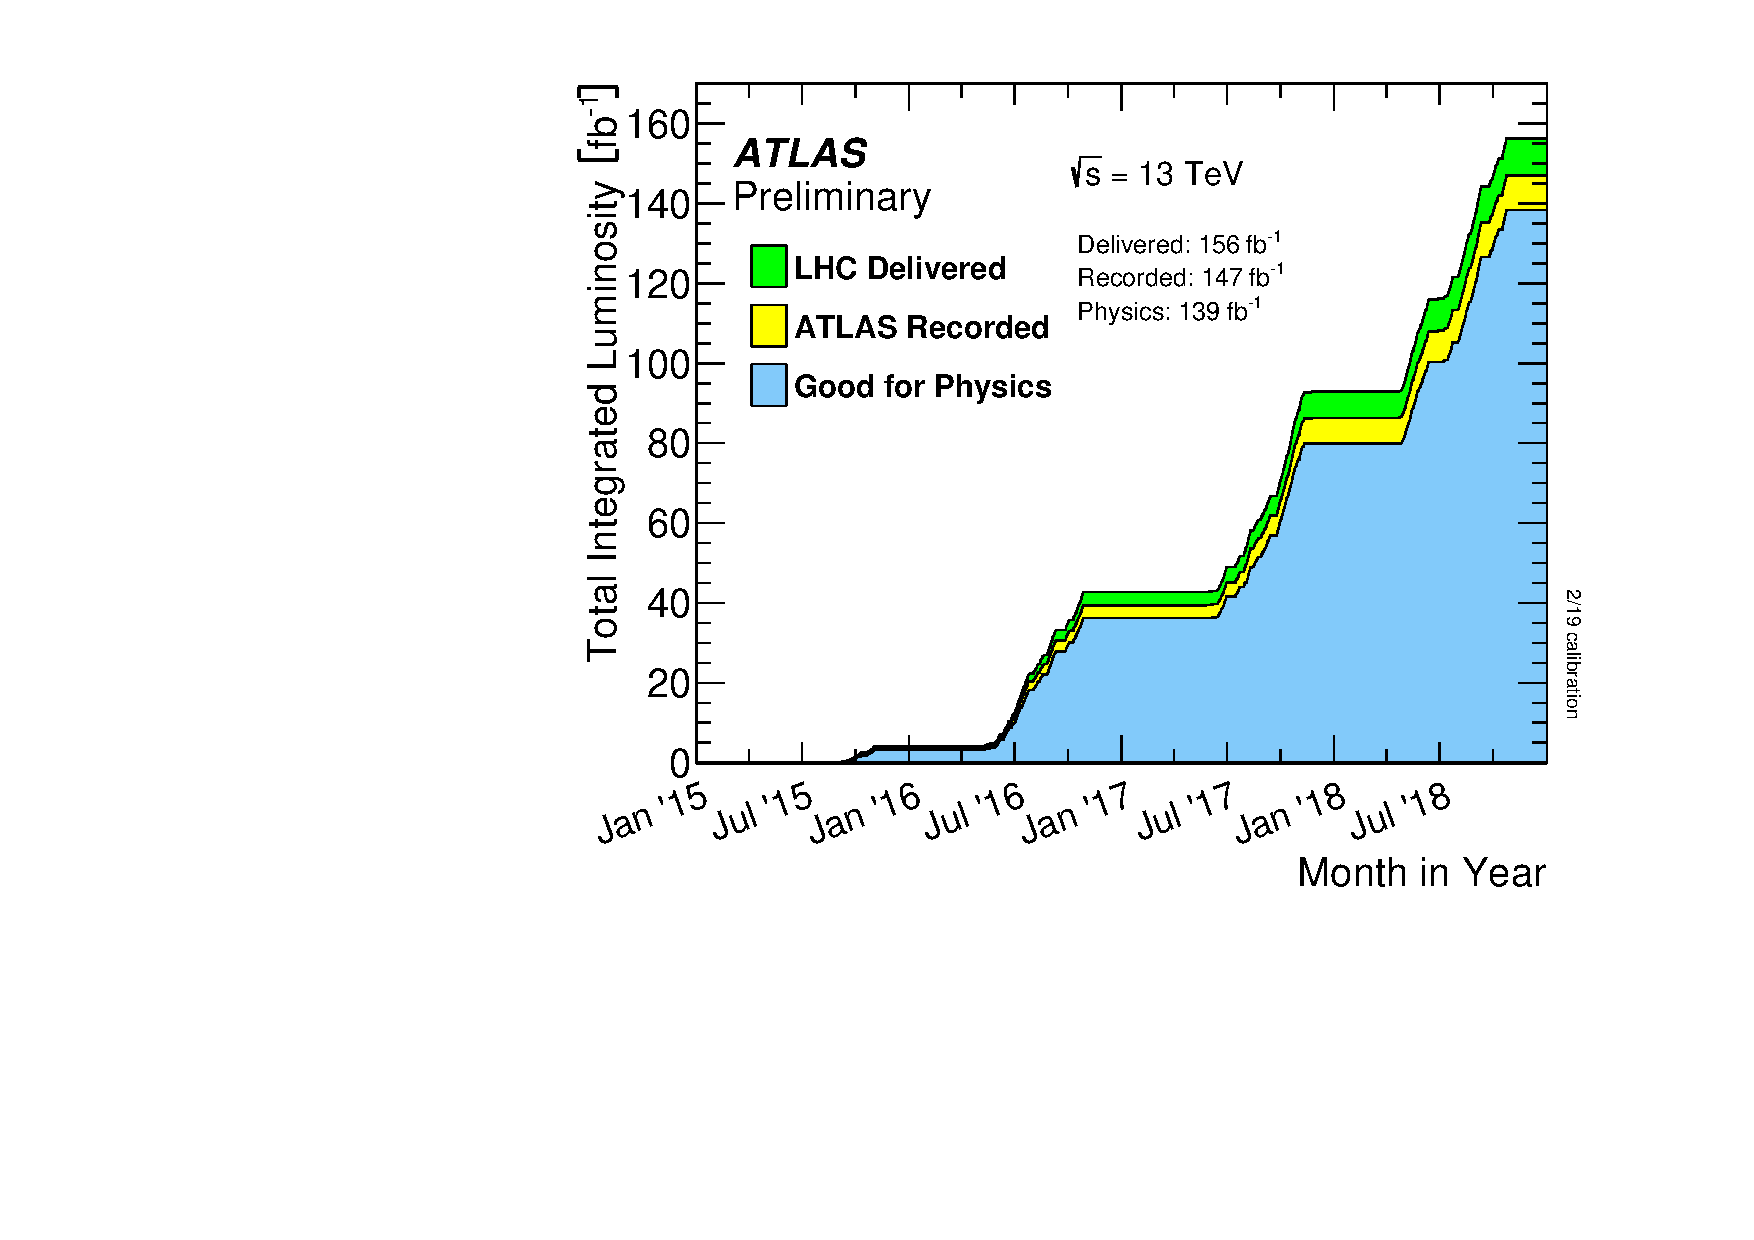
\includegraphics[width=0.6\textwidth]{figures/Detector/intlumivstimeRun2DQall.pdf}
  \caption{Integrated luminosity vs delivered month from 2015 to 2018 in ATLAS experiment.}
  \label{fig:lumi_vs_time}
\end{figure}

\textbf{Pile-up}

In collisions, multiple interactions can happen in one single bunch crossing, which is called ``\textit{pile-up}".
The variable $\left< \mu \right>$, representing the average number of interactions per bunch crossing that used to describe pile-up effect, is defined as:
\begin{equation}
    \left< \mu \right> = \frac{\mathcal{L}_{tot}\sigma}{f_{r}n_{bunch}}
\end{equation}
where $\mathcal{L}_{tot}$ is the instantaneous luminosity, $\sigma$ denotes the inelastic cross section,
$f_{r}$ represents the LHC revolution frequency and $n_{bunch}$ is the number of colliding bunches.
Usually, with increasing luminosity, the pile-up becomes more significant.
Figure~\ref{fig:run2_mu} shows the luminosity-weighted distribution of the mean number of interactions per crossing
for pp collision data from 2015 to 2018 (full run-2), the challenge of pile-up increased in each year.
\begin{figure}[!htb]
  \centering
  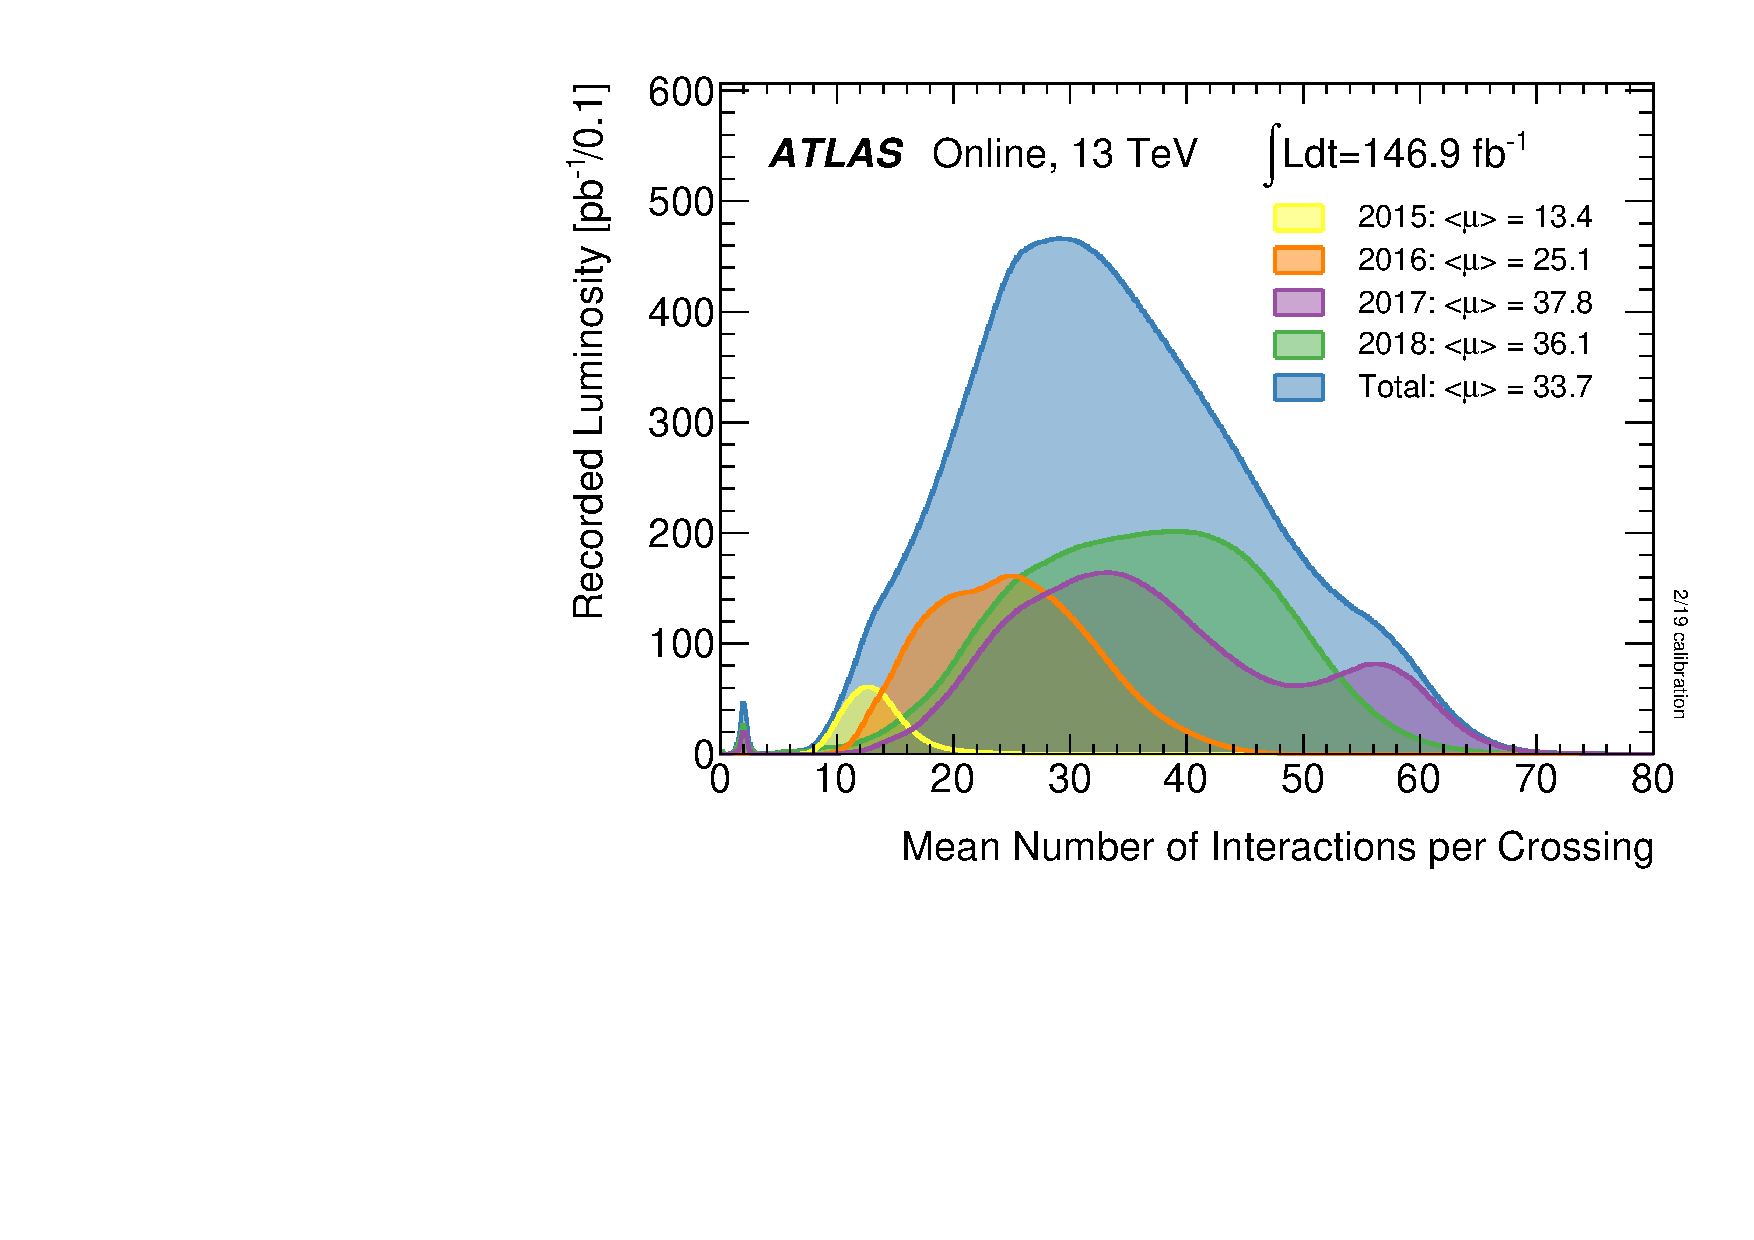
\includegraphics[width=0.6\textwidth]{figures/Detector/mu_2015_2018.pdf}
  \caption{Number of interactions per crossing weighted bt luminosity from 2015 to 2018 in ATLAS experiment.}
  \label{fig:run2_mu}
\end{figure}

%\subsection{Luminosity and pile-up}

\section{ATLAS detector}
\subsection{Detector overview}

ATLAS is the world's largest volume particle detector.
It is a cylinder with 46 meters long, 25 meters in diameter, and sits in a cavern 100 meters below ground.
The detector contains about 3000 km of cables and it weights 7000 tonnes.

The coordinate system and nomenclature used to describe the ATLAS detector \cite{Collaboration_2008} is depicted in figure~\ref{fig:coordinate}. We define the nominal interaction point as the origin of the coordinate system, the beam direction as the \textit{z}-axis and the \textit{x-y} plane is transverse to the beam direction.
The positive \textit{x}-axis is given as the direction from interaction point to the centre of the LHC ring, 
while the positive \textit{y}-axis points upward.
\begin{figure}[!htb]
  \centering
  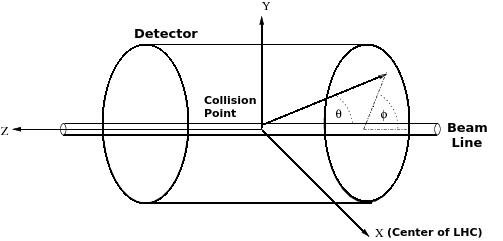
\includegraphics[width=0.9\textwidth]{figures/Detector/Coordinate_system_atlas.png}
  \caption{Coordinate system used by the ATLAS experiment at the LHC \cite{Perez:phdthesis}.}
  \label{fig:coordinate}
\end{figure}
There are two sides of detector A and C, in which A (C) -side is in the positive (negative) \textit{z} direction.
The polar angle $\theta$ is measured from the beam axis, while the azimuthal angle $\phi$ is obtained around the beam axis.
In physics analysis, we usually use the pseudorapidity $\eta$ designed as:
\begin{equation}
    \eta = - ln \left[ tan\left( \frac{\theta}{2}\right) \right]
\end{equation}
instead of $\theta$ angle. 
And for massive objects (eg. jets), the rapidity is used:
\begin{equation}
    y = \frac{1}{2} ln \left[ \frac{E+p_{z}}{E-p_{z}} \right]
\end{equation}

In addition, the transverse momentum $p_{T}$, transverse energy $E_{T}$ and the missing transverse energy $E_{T}^{miss}$ are defined in \textit{x-y} plane.
The $\Delta R$, a commonly used distance measurement, is defined in the pseudorapidity-azimuthal angle space as:
\begin{equation}
    \Delta R = \sqrt{ \Delta\eta^{2} + \Delta\phi^{2}}.
\end{equation}

The overall ATLAS layout is shown in figure~\ref{fig:atlas_layout}, which is forward-backward symmetric with respect to the interaction point.
\begin{figure}[!htb]
  \centering
  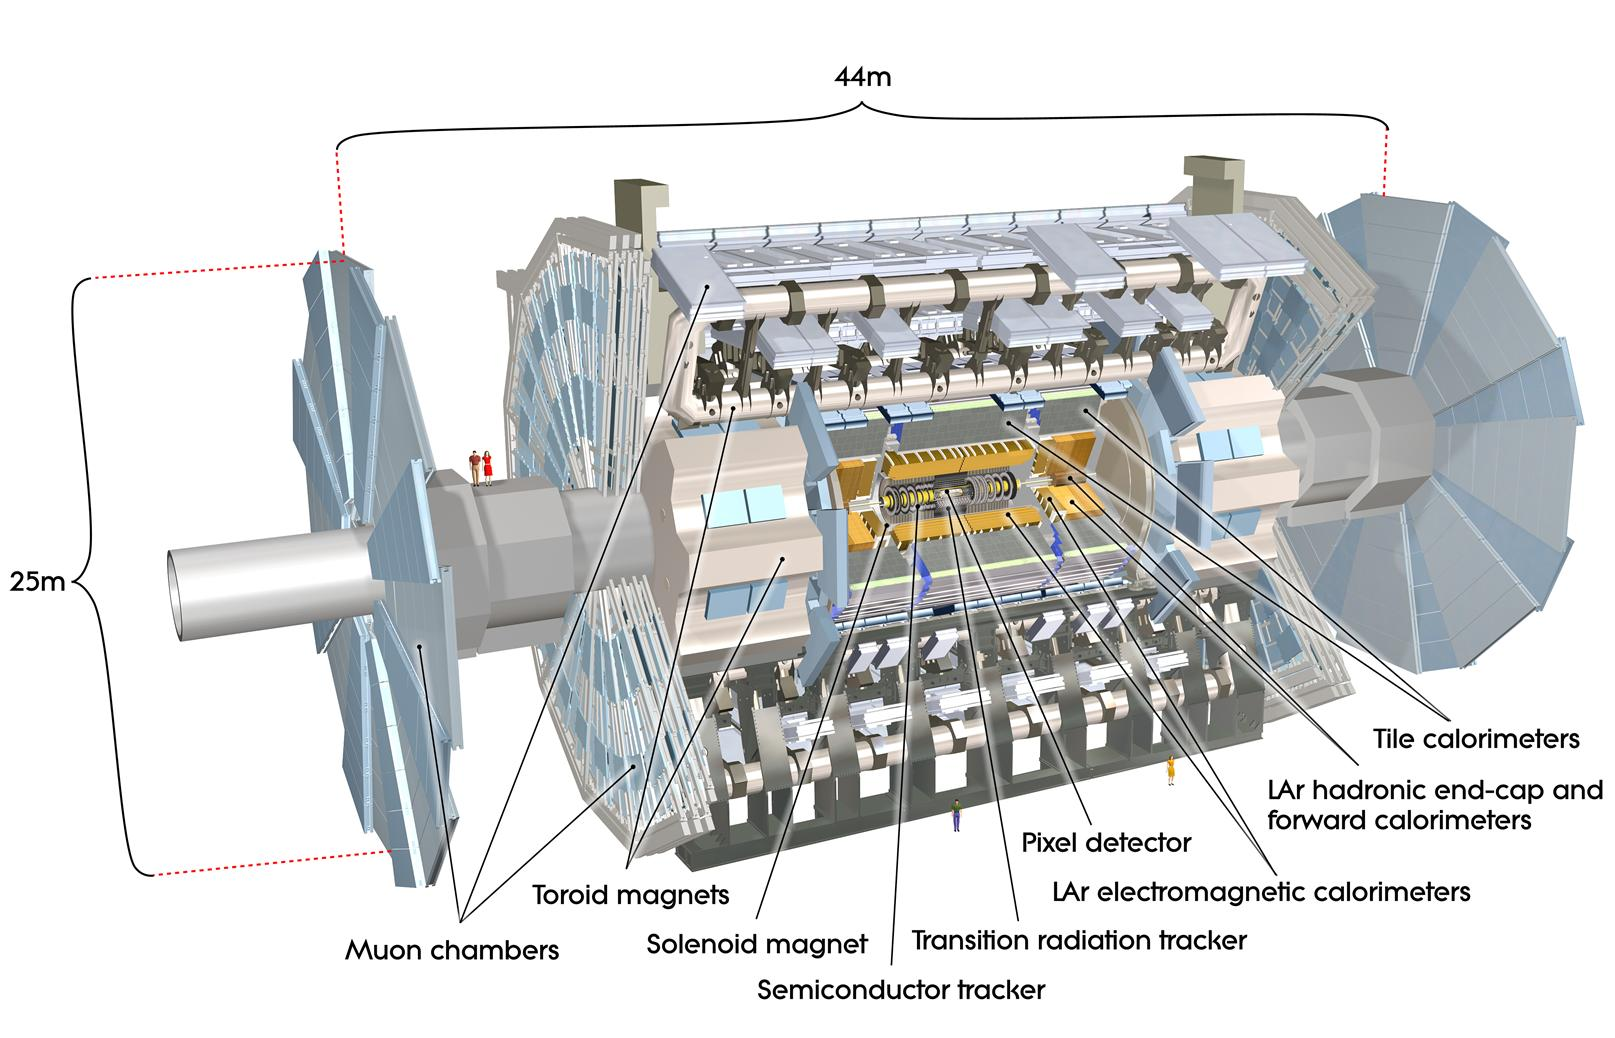
\includegraphics[width=1.0\textwidth]{figures/Detector/atlas_layout.jpg}
  \caption{Layout view of the ATLAS detector \cite{Pequenao:1095924}.}
  \label{fig:atlas_layout}
\end{figure}
The magnet configuration has a thin superconducting-solenoid surrounding the inner-detector, 
and three large superconducting-toroids (one barrel and two end-caps) around the calorimeters.

\textbf{The inner detector}, which is the innermost part of ATLAS, is surrounded by a 2 T solenoidal magnetic field.
It's used for pattern recognition, momentum and vertex measurements and electron identification, with the combination of tracking system in the region of $\eta$ up to 2.5.

\textbf{The calorimeter} is outside the solenoid, for electromagnetic and hadronic energy measurements.
The high granularity liquid-argon (LAr) electromagnetic sampling calorimeters is used to measure energy and position with range up to $|\eta| < 3.2$ for electrons and photons.
For hadron, a scintillator-tile calorimeter is used in the range of $|\eta| < 1.7$, and the liquid-argon hadronic endcap calorimeters (HEC) is used in end-cap region.
And then the LAr forward calorimeters provide both electromagnetic and hadronic energy measurements with the coverage in forward region up to $|\eta| = 4.9$.

\textbf{The muon spectrometer} is the outermost layer.
It's a air-core toroid system, with a long barrel and two inserted end-cap magnets that provides strong bending power in a large volume within a light and open structure.
A set of chambers measuring the tracks of muons with high spatial precision and accurate time-resolution are used.
Multiple-scattering effects are minor, and excellent muon momentum resolution can be achieved.

%\subsection{Dector overview}

\chapter{Simulation and Object Reconstruction for the ATLAS Experiment}

In current LHC pp collison, bunches of protons collide every 25 nanoseconds (ns), which gives a large challenge to event reconstruction and selections.
To predict and model each process, the Monte Carlo simulations of physics events are essential for high-energy physics experiments.
This section will briefly discuss the event simulation and reconstruction programs based on the ATLAS software framework. 

\section{Event sumilation}
%\subsection{Simulation framework}

The ATLAS simulation program is integrated into the ATLAS software framework called \textit{Athena}~\cite{atlas:athena},
which uses Python as an object-oriented scripting and interpreter language to configure and load C++ algorithms and objects.
Figure~\ref{fig:frame_overview} shows the overview of ATLAS simulation data flow~\cite{Aad:2010ah}.
In the diagrams, the square-cornered boxes represents algorithms and applications to be run and round-cornered boxes denote data objects.
\begin{figure}[!htb]
  \centering
  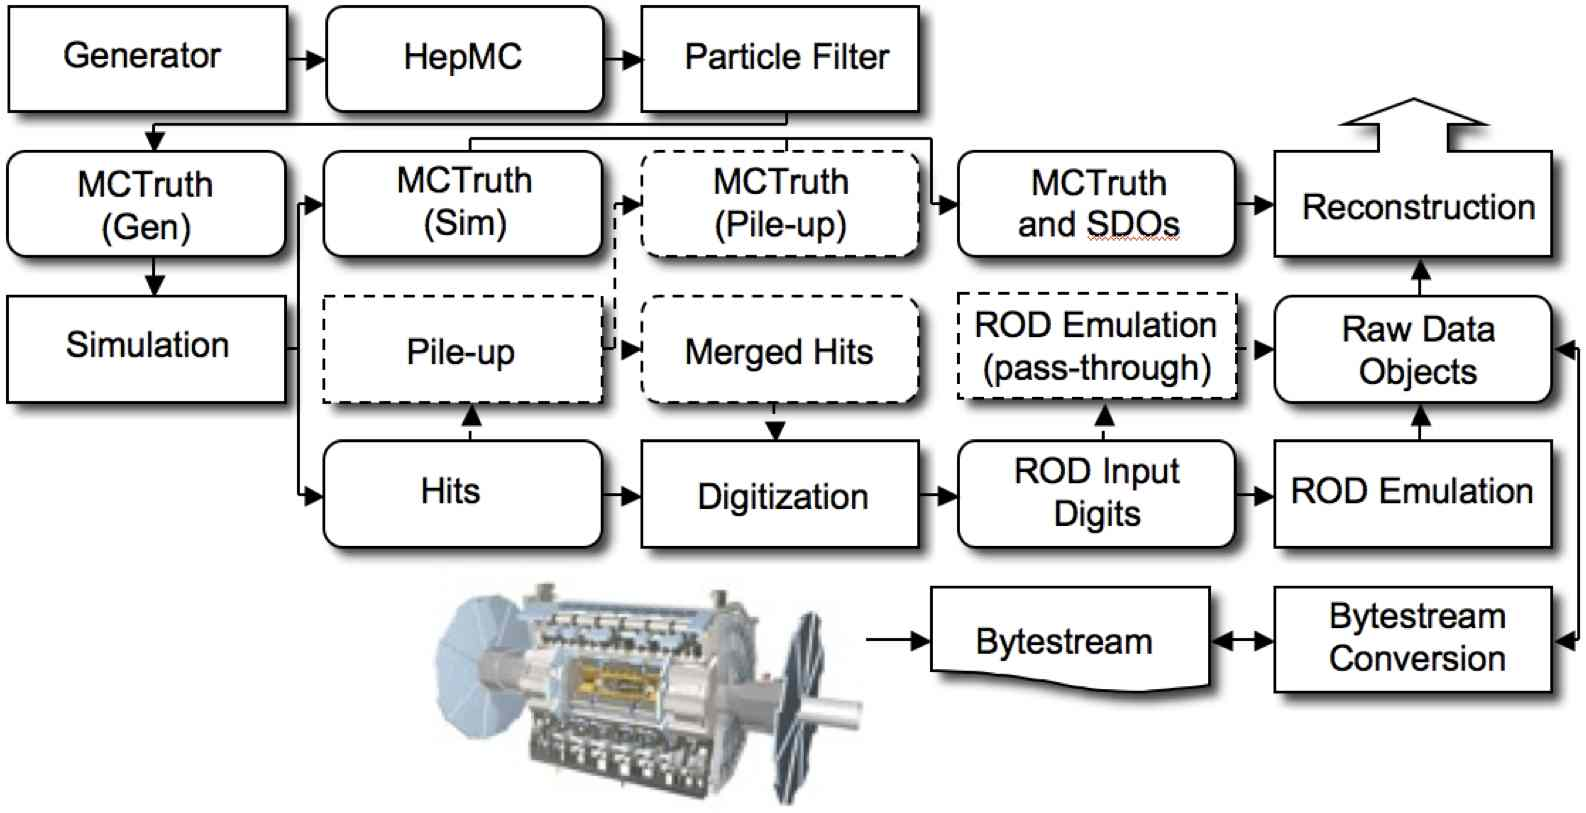
\includegraphics[width=1.0\textwidth]{figures/Simulation/outline_atalsSimulation_v2.png}
  \caption{The flow of the ATLAS simulation software.}
  \label{fig:frame_overview}
\end{figure}

First of all, events are produced by MC generators in standard HepMC format and then read into the simulation.
During the simulation, particles are propagated through the full ATLAS detector whose configurations can be set by users via GEANT4 toolkit.
The energies deposited in the sensitive regions of the detector are recorded as \textit{hits} that contains the total energy deposition,
position and time, and are written to a simulation hit file.
In the meatime, the events in "truth" format are also recorded to contain the history of the interactions from the generator, including incoming and outgoing particles.
Simulated Data Objects (SDOs) are created from truth, which are maps between hits in sensitive portions of the detector and truth information of particles in simulation.
The files are then sent to digitization, with constructs ``digits" inputs and be written into Raw Data Object (RDO) file used for reconstruction.

In conclusion, there are three main parts of framework: \textit{Generation}, \textit{Simulation} and \textit{Digitization}.
More details are given as below:

\textbf{Event generation}

As shown in figure~\ref{fig:mc_event_structure}~\cite{Hoche:2014rga}, at hardon colliders, multiple scattering and rescattering effects arise, which needs to be simulated by Monte Carlo (MC) event generators to reflect the full complexity of those event structures.
Several MC event generators can be used to generate events originally in HepMC format.
The events can be filtered at generation time with some certain requirements (eg. decay channel or missing energy above a certain threshold).
The generator is responsible for any prompt decays (e.g. W or Z bosons) but stores any "stable" particle expected to propagate through a part of the detector. 
During the generation steps, any interactions with detector are ignored and only immediate decays are considered.

There are several MC generators that have been widely used with general purpose, which include \textsc{Sherpa}~\cite{Gleisberg_2009}, \textsc{Herwig++}~\cite{Bahr2008}, \textsc{PowhegBox}~\cite{Nason:2004rx}, \textsc{MC@NLO}~\cite{Frixione_2002} and \textsc{Pythia8}~\cite{Sjostrand:2007gs}.

\begin{figure}[!htb]
  \centering
  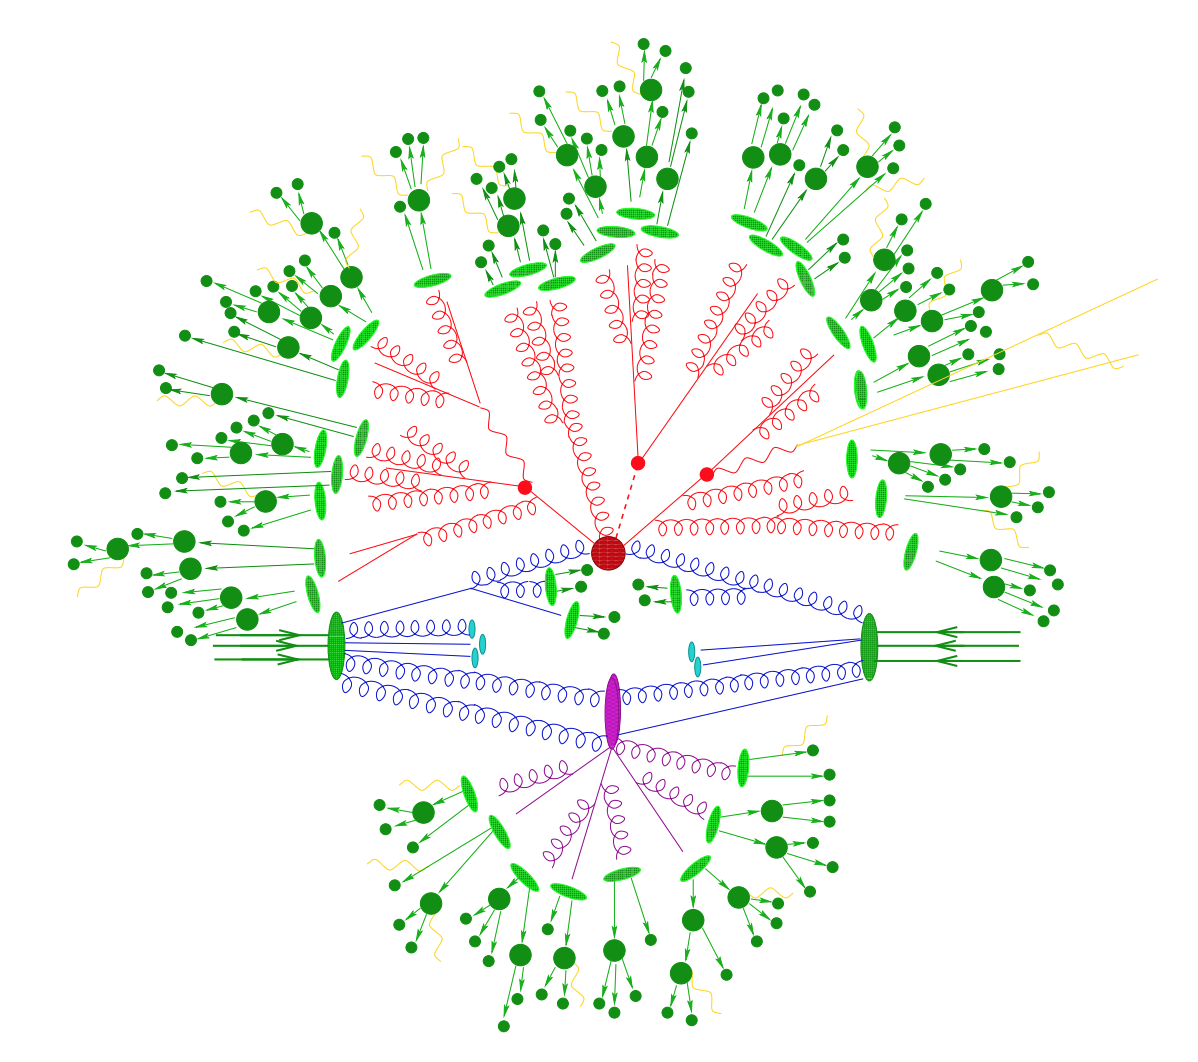
\includegraphics[width=0.7\textwidth]{figures/Simulation/mc_event_structure.png}
  \caption{Sketch of a hardon-hardon collision simulated by MC event generator. The red blob in center denotes the hard collision, surrounded by tree-like structures representing Bremsstrahlung which is simulated by Parton Showers. The purple blob stands for a secondary hard scattering event. The light green blobs indecate the parton-to-hardon transitions and the dark green blobs represents hardon decays. The yellow lines are soft photon radiations.}
  \label{fig:mc_event_structure}
\end{figure}

\textbf{Simulation}

GEANT4 is used as standard simulation toolkit for the ATLAS experiment, which transports physics particles through the detector's geometry.
During the generation level, the entire connected chain of the HepMC event is stored as the Monte Carlo truth. 
Only the stable particles are read into GEANT4 for further simulation and selection, while transformations can be applied to these events to select certain processes.
During the simulation, many secondary tracks can be produced, therefore only information from the interactions of interest are stored, including the incoming particles, step sequence, vertex as well as outgoing particles.
The output of GEANT4 is called \textit{hit file}, which contains metadata describing the configuration of the simulation during the run, all truth information requested and a collection of hits for each subdetector.

Since the standard ATLAS detector simulation cost very large computing resources to accurately model the complex detector geometry and physics descriptions, some fast simulation programss are developed according to different user purpose.
Some popular fast-sim toolkits include \textit{Fast G4 Simulation}~\cite{Barberio:2007gba}, \textit{ATLFAST-I}~\cite{Richter-Was:683751} and \textit{ATLFAST-II}~\cite{Edmonds:1091969}.

\textbf{Digitization}

The hit outputs from simulated events, including hard scattering signal, minimum bias, beam halo, beam gas and cavern background events, are then sent into digitization procedure, converted into detector response called ``digits".
Before converted into detector signal as `digits' formart, each type of event can be overlaid at a user-specified rate.
Those overlay, called ``pile-up", can be done during degitization to save the CPU time.
At this stage, the detector noise and the first level trigger that implemented with hardware on the real detector are added into events.
The digitization firstly constructs ``digits" inputs to the readout drivers (RODs) in the detector electronics.
Then the ROD functionality is emulated, and the output digits are written out as Raw Data Object (RDO) file.
In addition, the digitization algorithms can also produce Simulated Data Objects (SDOs), which contain information about all the particles, noise and the amount of energy that contributed to the signal. 
Then all information are sent into reconstruction level described in next subsection.

%\subsection{Simulation framework}

\chapter{Observation of electroweak ZZ production and measurement of SM ZZ cross section}

\section{Introduction}

After the discovery of Higgs boson~\cite{20121, 201230}, the examination of electroweak symmetry breaking (EWSB) becomes a main focus at the LHC.
In addition to measuring the properties of Higgs boson directly, the vector boson scattering (VBS) process is another key avenue to probe EWSB~\cite{Lee:1977yc, Chanowitz:1985hj, Szleper:2014xxa}.
As introduced in section~\ref{symbreaking}, in Standard Model (SM), the Higgs boson acts as ``moderator" to unitarize high-energy longitudinal VBS amplitudes at the ~\tev~ scale.
Therefore, studying high-energy behaviours of VBS is crucial to understand the mechanism of EWSB.

Since no VBS process was observed prior to the LHC era, LHC provides an exceptionable opportunity to study them due to its unprecedented high energy and luminosity.
At the LHC, the VBS process is typically studied through the measurements of electroweak (EW) production of two vector bosons radiated from quark-quark initial state, 
plus a pair of hadronic jets with high energy in the back and forward regions (denoted as EW-$VVjj$).
The quantum chromodynamics (QCD) production of $VVjj$ containing two QCD vertices at the lowest order (denoted as QCD-$VVjj$) is an irreducible background to the search of EW-$VVjj$ production.
The features of EW-$VVjj$ production including a large invariant mass of jet pair ($m_{jj}$) and a significant separation of rapidity between two jets ($\Delta y_{jj}$).
Figure~\ref{fig:vbszz_diagrams} presents some typical Feynman diagrams of EW- and QCD- $ZZjj$ processes.
\begin{figure}[!htbp]
\begin{center}
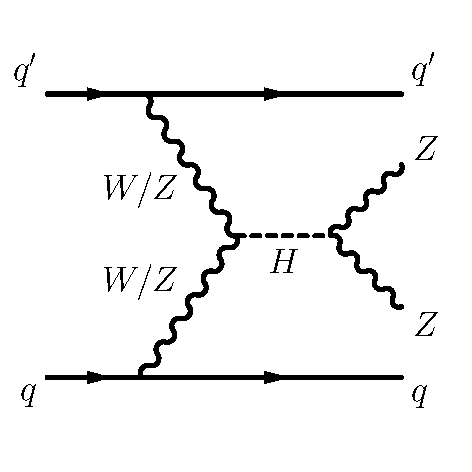
\includegraphics[width=0.22\textwidth]{figures/VBSZZ/diagram-EWZZjj-Schn-Higgs.pdf}
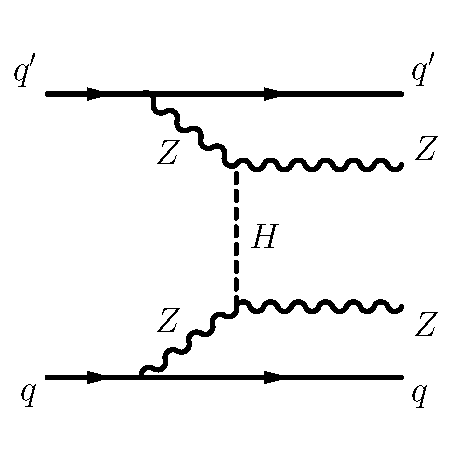
\includegraphics[width=0.22\textwidth]{figures/VBSZZ/diagram-EWZZjj-Tchn-Higgs.pdf}
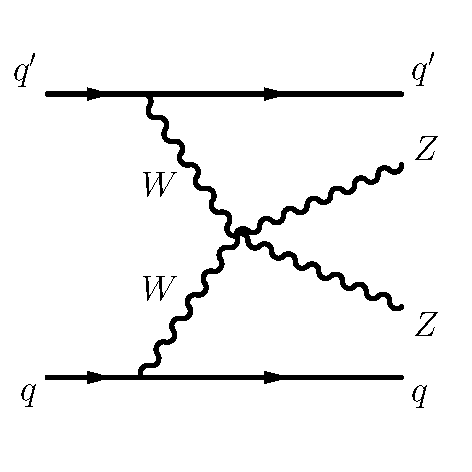
\includegraphics[width=0.22\textwidth]{figures/VBSZZ/diagram-EWZZjj-QGC.pdf}
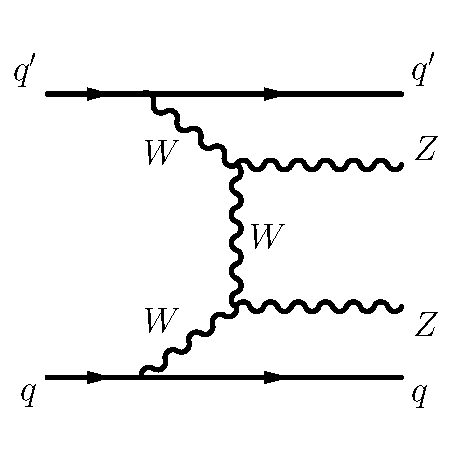
\includegraphics[width=0.22\textwidth]{figures/VBSZZ/diagram-EWZZjj-TGC.pdf}\\
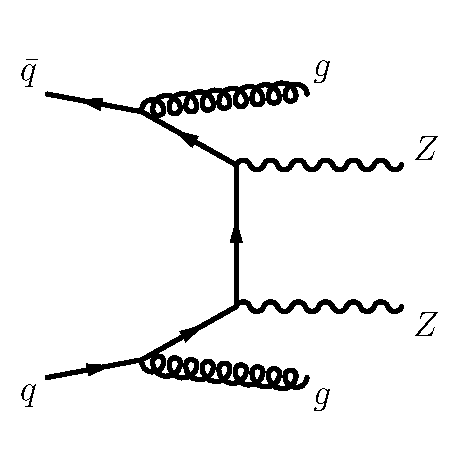
\includegraphics[width=0.22\textwidth]{figures/VBSZZ/diagram-QCDZZjj-qq.pdf}
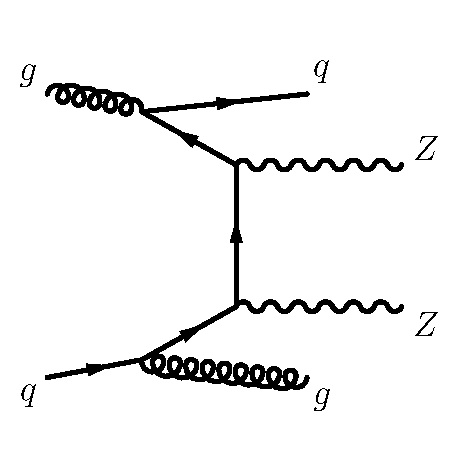
\includegraphics[width=0.22\textwidth]{figures/VBSZZ/diagram-QCDZZjj-qg.pdf}
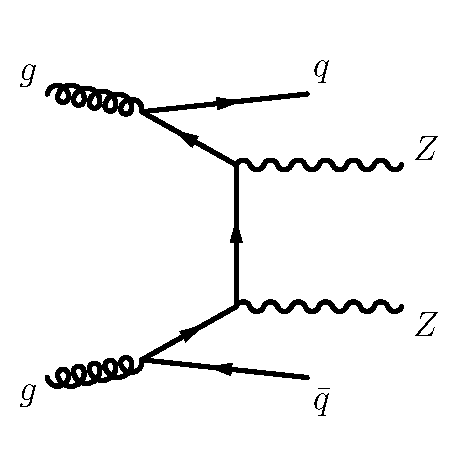
\includegraphics[width=0.22\textwidth]{figures/VBSZZ/diagram-QCDZZjj-gg.pdf}
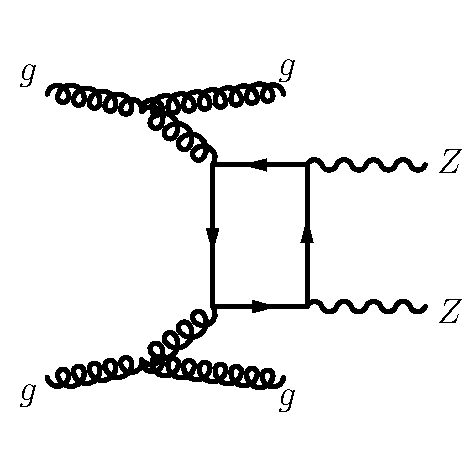
\includegraphics[width=0.22\textwidth]{figures/VBSZZ/diagram-QCDZZjj-box.pdf}\\
\end{center}
\caption{Typical diagrams for the production of $ZZjj$, including the relevant EW VBS diagrams (first row) and QCD diagrams (second row).}
\label{fig:vbszz_diagrams}
\end{figure}

The first evidence of the EW-$VVjj$ process was seen in same-sign $WW$ channel (EW-$W^{\pm}W^{\pm}jj$) by ATLAS collaboration with 20.3~\ifb~8~\tev~data~\cite{PhysRevLett.113.141803},
in which a 3.6$\sigma$ excess was observed in data over the background-only prediction.
In the LHC run-2, the observation (with > 5 $\sigma$ statistical significance) of EW-$W^{\pm}W^{\pm}jj$ process has been reported in both ATLAS and CMS collaboration with 36~\ifb~13~\tev~data\cite{PhysRevLett.123.161801, Sirunyan:2017ret}.
In $WZ$ channel (EW-$WZjj$), an observation with 5.3 $\sigma$ excess was also reported by the ATLAS collaboration recently~\cite{2019469}.
As for the EW-$ZZjj$ production, it was searched by CMS using 35.9~\ifb~13~\tev~data but no evidence was found\cite{2017682}.
The EW production in $ZZ$ final state (EW-$ZZjj$) is typically rare, whose fiducial cross section has an order of \textit{O}(0.1)~\ifb in the final state where both $Z$ bosons decay leptonically.
But in the meantime, $ZZ \rightarrow \llll$ process offers an extremely clean channel than all the others. So with more data collected in the LHC, the observation of EW-$ZZjj$ becomes possible.

This section presents the first observation of EW-$ZZjj$ production decaying to four charged leptons with two jets (\lllljj) by ATLAS collaboration using the complete set of the LHC run-2 data with 139~\ifb luminosity~\cite{Aad:2020zbq,Zhu:2714092}.
It is a new milestone in the study of EWSB at the LHC, and completes the last missing part of observation of weak boson scattering for massive bosons.
In the meatime, the measurement of fiducial cross-sections for SM $ZZ$ production including both EW and QCD processes is also reported.
The $ZZjj$ production involving intermediate $\tau$-leptons from $Z$ decays is considered as signal but has a negligible contribution to the selected events.
Reducible backgrounds give minor contributions in the \lllljj channel are also studied.
To further separate the EW signal and the QCD background, multivariate discriminant (MD) is trained using event kinematic information from simulated samples. 
The MD distribution is then used as discriminant in statistical fit to evaluate the signal strength of EW process.

\section{Data and MC samples}

\subsection{Data samples}

The data sets for this analysis are the full run-2 pp collision data collected by the ATLAS experiment during the years from 2015 to 2018.
Data event is only used if it passed the latest Good Run List (GRL) released by the Data Quality group from ATLAS experiment as listed below:


{\tiny
\begin{verbatim}
data15_13TeV.periodAllYear_DetStatus-v89-pro21-02_Unknown_PHYS_StandardGRL_All_Good_25ns.xml
data16_13TeV.periodAllYear_DetStatus-v89-pro21-01_DQDefects-00-02-04_PHYS_StandardGRL_All_Good_25ns.xml
data17_13TeV.periodAllYear_DetStatus-v99-pro22-01_Unknown_PHYS_StandardGRL_All_Good_25ns_Triggerno17e33prim.xml
data18_13TeV.periodAllYear_DetStatus-v102-pro22-04_Unknown_PHYS_StandardGRL_All_Good_25ns_Triggerno17e33prim.xml
\end{verbatim}
}

The events are required to additionally recorded by single and multi-lepton triggers, with transverse momentum ($p_{T}$) thresholds varing from 8 to 26 GeV.
The overall trigger efficiency for selected inclusive \llll jj signal events in the analysis region are from 95 to 99\%.

%% =======================================================
\subsection{MC simulation}

The EW-ZZjj production (signal) is modelled using \MGMCatNLO~2.6.1~\cite{Alwall:2014hca} matrix elements (ME) calculated in the leading-order (LO) approximation
in perturbative QCD (pQCD) and with NNPDF2.3LO~\cite{Ball:2012cx} parton distribution functions (PDF).
VBF Higgs process is also included.

The QCD-ZZjj production is modelled using \textsc{Sherpa} 2.2.2~\cite{Gleisberg:2008ta} with the NNPDF3.0NNLO~\cite{ball2015parton} PDF,
in which events with up to one (three) outgoing partons are generated at NLO (LO) in pQCD.
The production of ZZjj from the gluon-gluon initial state with a four-fermion loop or with an exchange of the Higgs boson has an order of $\alpha_{S}^{4}$ in QCD,
and is not included in the \textsc{Sherpa} simulation.
A separate $gg$ induced $ZZ$ + 2jets sample is modelled using \textsc{Sherpa} 2.2.2 with the NNPDF3.0NNLO PDF,
and with an additional 1.7 k-factor~\cite{PhysRevD.92.094028} being applied.

Then the interference between EW- and QCD-ZZjj is modelled with \MGMCatNLO~2.6.1 calculated at LO.

The diboson productions from QCD $WW \rightarrow lvqq$ as well as QCD and EW $WZ \rightarrow llqq$ are modelled using \textsc{Sherpa} 2.2.2 with NNPDF3.0NNLO PDF.
The productions of semileptonic decays ($WW \rightarrow lvqq$ and $WZ \rightarrow qqll$) are modelled using \textsc{Powheg-Box}~v2~\cite{Frixione:2007nw} with the CT10 PDF~\cite{Lai:2010vv}.
Other diboson processes are not included due to negligible contributions.
The triboson production is modelled using \textsc{Sherpa} 2.2.2 with NNPDF3.0NNLO PDF.

For top-quark pair (\ttbar) production, the \textsc{Powheg-Box}~v2 is used with the CT10 PDF.
The single top-quark production in $t$-channel, $s$-channel and $Wt$-channel were simulated using the \textsc{Powheg-Box}~v1 event generator~\cite{Alioli:2009je,Frederix:2012dh,Re:2010bp}.
The productions of \ttbar~in association with vector boson(s) ($ttV$) is modelled with \MGMCatNLO~2.3.3 for $ttW$ and $ttZ$ with $Z \rightarrow \nu\nu/qq$ decays,
with \textsc{Sherpa} 2.2.1 for $ttZ$ with the $Z$ to dilepton decays,
and with \MGMCatNLO~2.2.2 for $ttWW$ respectively.

The \Zjet processes are modelled using \textsc{Sherpa} 2.2.1 with NNPDF3.0NNLO PDF, 
in which the ME is calculated for up to two partons with next-to-leading-order (NLO) accuracy in pQCD and up to four partons with LO accuracy.

For all the samples except those from \textsc{Sherpa}, 
the parton showering is modelled with \textsc{Pythia8}~\cite{Sjostrand:2007gs} using NNPDF2.3~\cite{Ball:2012cx} PDF set,
and the A14 set of tuned parameters~\cite{ATL-PHYS-PUB-2014-021}.
For \textsc{Sherpa} samples, the parton showering is simulated within the programme.

All simulated events were processed with detector response simulated based on \textsc{Geant4} described in section~\ref{sec:simulation_framework}.
In addition, simulated inelastic pp collisions were overlaid to model additional pp collisions in the same and neighbouring bunch crossings (pile-up),
and reweighted to match the pile-up conditions in data.
Moreover, all simulated events were processed using the same reconstruction algorithms as data.
And the leptons' and jets' reconstruction, energy scale and resolution, and the leptons' identification, isolation, trigger efficiencies for simulated events,
as described in section~\ref{sec:reconstruction}, were all corrected to match the data measurements.

\section{Objects and Event selection}
\label{sec:selection}

\subsection{Objects selection}

The selection of analysis relies on the defination of multiple objects: \textit{electrons}, \textit{Muons}, and \textit{jets}.
Details of definations for each objects are described as below:

\textbf{Muon:} 
To increase the acceptance range in reco-level for \llll jj channel, all four types of muons 
(CB, ST, CT, ME muons, described in section~\ref{sec:muon}) are used.
The identified muons are then required to pass $p_{T} > 7 \gev$ and $|\eta| < 2.7$,
and satisfy the \textit{Loose} identification criterion (see defination in sec~\ref{sec:muon}).
The impact parameter cuts are further applied to suppress the contribution from cosmic muons and non-prompt muons,
with the value of: $|d_{0}/\sigma(d_{0})| < 3.0$ and $|z_{0} sin\theta| < 0.5 mm$,
where $d_{0}$ is the transverse impactparameter relativetothebeamline, $\sigma(d_{0})$ is its uncertainty, 
and z0 is the longitudinal impactparameter relative to the primary vertex.
In order to avoid muons associated with jets, all muons are required to be isolated and pass \textit{FixedCutLoose} isolation criteria,
which required $E_{T}^{topocone20} / p_{T} < 0.3$ and $p_{T}^{varcone30} / p_{T} < 0.15$.

\textbf{Electron:} 
As described in section~\ref{sec:electron}, electrons are reconstructed from energy deposits in the EM calorimeter matched to a track in the inner detector.
The electron candidates must satisfy the \textit{Loose} criterion valuing by the likelihood-based (LH) method.
And electrons are required to have $p_{T} > 7 \gev$ and $|\eta| < 2.47$.
Moreover, the impact parameter requirements of $|d_{0}/\sigma(d_{0})| < 5.0$ and $|z_{0} sin\theta| < 0.5 mm$ are applied.
Same as muon, all electrons are required to satisfy \textit{FixedCutLoose} isolation criteria
of $E_{T}^{cone20} / p_{T} < 0.2$ and $p_{T}^{varcone20} / p_{T} < 0.15$.

\textbf{Jets:} 
Jet are key signatures for VBS processes. 
This analysis use the jets clustered using the anti-kt algorithm with radius parameter R = 0.4, more details of jets' reconstruction can be found in section~\ref{sec:jet}.
The jets are reuiqred to have $\pT >$ 30 (40)~\gev~in the $|\eta| <$ 2.4 ($2.4 < |\eta| < 4.5)$ region.
To further reduce the effects of pile-up jets, a jet vertex tagger (JVT) is applied to jets with $p_{T} <$ 60~\gev~and $|\eta| < 2.4$ to select jets from hard-scattering vertex.

\textbf{Overlap removal:} 
An overlap-removal procedure is applied to selected leptons and jets in this analysis.
To enhance the selection efficiency, leptons are given higher priority to be kept when overlaping with jets.
With this lepton prefered mothed, the events of EWK signal after selection increases about 19\% while background only increases \~ 14\%.
More details of the strategy is summarized in table~\ref{tab:OR_4l}.
\begin{table}[htbp]
\begin{center}
\renewcommand\arraystretch{1.8}
\resizebox{\linewidth}{!}{
\small
\begin{tabular}{ l | c | c}
\hline
\centering & Reference objects & Criteria\\
\hline \hline
Remove electrons & electrons & Share a track or have overlapping calorimeter cluster. Keep higher \pt electron \\
\hline
Remove muons & electrons & Share track and muon is calo-tagged \\
\hline
Remove electrons & muons & Share track \\
\hline
\multirow{3}{*}{Remove jets} & electrons & $\Delta R_{e-jet}$ < 0.2  \\
\cline{2-3}
                   & \multirow{2}{*}{muons}     & $\Delta R_{\mu-jet}$ < 0.2 OR muon track is ghost-associated to jet \\
                   &       &  \textbf{AND} ($N_{Trk}(jet)<3$ OR ($p_T^{jet}/p_T^{\mu}<2$ and $p_T^{\mu}/\Sigma_{TrkPt}>0.7$)) \\
\hline\hline
\end{tabular}}
\end{center}
\caption{Overlap removal criteria between pre-selection objects for the \llll channel. The overlap removal follows the order shown in this table. Once an object has been marked as removed, it does not participate in the subsequent stages of the overlap removal procedure. }
\label{tab:OR_4l}
\end{table}

%% ========================================================================
\subsection{Event selection in reconstruction level}

The \llll quadruplets are formed by two opposite-sign, same-flavour (OSSF) lepton pairs ($l^{+}l^{-}$),
in which leptons are required to be separated by $\Delta R > 0.2$ in table~\ref{tab:OR_4l}.
At most one muon is allowed to be ME or CT muon.
The $\pT$ threshold of first three leading muons are 20, 20 and 10~\gev.
If more than one quadruplets are found, the one with minimum sum of difference between two muon pair masses and Z boson mass 
($|m_{l_{1}^{+}l_{1}^{-}} - m_{Z}| + |m_{l_{2}^{+}l_{2}^{-}} - m_{Z}|$) is selected.
Both two dilepton pair masses are required to between 66 to 116~\gev.
In addition, the invariant masses of all possible OSSF pairs are required to be greater than 10 \gev to reject events from $J/\phi$ or $\Upsilon$ decay.

For VBS topology, the two most energetic jets in different detector side ($y_{j1} \times y_{j2} < 0$) are selected.
Furthermore, the invariant mass of two jets ($\mjj$) is required to be greater than 300~\gev, 
while $\dyjj$ is required to be larger than 2.
Table~\ref{tab:selection_reco} summarizes the above selection requirements, which is defined as signal region (SR).

\begin{table}[!htbp]
\begin{center}
\scalebox{0.75} {
\begin{tabular}{c c}
\hline
\hline \noalign{\smallskip}
\multirow{2}{*}{Electrons}     & $\pT >$ 7~\GeV{}, $|\eta| <$ 2.47            \\
                     & $|d_0/\sigma_{d_0}|<5$ and $|z_0\times\sin\theta|<0.5$ mm                                                             \\
\noalign{\smallskip}\hline\noalign{\smallskip}
\multirow{2}{*}{Muons}         & $\pT >$ 7~\GeV{}, $|\eta| <$ 2.7             \\
                     & $|d_0/\sigma_{d_0}|<3$ and $|z_0\times\sin\theta|<0.5$ mm                                                              \\
\noalign{\smallskip}\hline\noalign{\smallskip}
Jets                 & $\pT >$ 30 (40)~\GeV{} for $|\eta| <$ 2.4 ($2.4<|\eta|<4.5$)       \\
\noalign{\smallskip}\hline\noalign{\smallskip}
\multirow{5}{*}{$ZZ$ selection}  & $\pT >$ 20, 20, 10~\GeV{} for the leading, sub-leading and third leptons      \\
                     & Two OSSF lepton pairs with smallest $|m_{\ell^+\ell^-} - m_Z| + |m_{\ell^{'+}\ell^{'-}} - m_Z|$      \\
                     & $m_{\ell^+\ell^-} >$ 10~\GeV{} for lepton pairs                                            \\
                     & $\Delta R(\ell,\ell') >$ 0.2                                                               \\
                     & 66 $< m_{\ell^+\ell^-} <$ 116~\GeV{}                                                       \\
\noalign{\smallskip}\hline\noalign{\smallskip}
\multirow{2}{*}{Dijet selection}  & Two most energetic jets with $y_{j_1} \times y_{j_2} < 0$                                \\
                     & $\mjj >$ 300~\GeV{} and $\dyjj >$ 2                                                         \\
\noalign{\smallskip}\hline
\hline
\end{tabular}}
\end{center}
\caption{Summary of selection of physics objects and candidate events at detector level in the \lllljj signal region.}
\label{tab:selection_reco}
\end{table}
%Besides, a QCD Control region (CR) is defined by reverting either the $\mjj$ or $\dyjj$ requirements. 


\section{Background estimation}
\label{sec:background}

Table~\ref{tab:yield_prefit} summarizes the background yields for $ZZjj \rightarrow \lllljj$ channel in 139~\ifb.
Uncertainties on the predictions include both statistical and systematic components.
"Others" includes minor contributions from non-$ZZ$ processes including \Zjet, top-quark, triboson and $ttV$ processes.
Detail of estimation for each source will described below.

\begin{table}[!htbp]
\sisetup{
table-number-alignment = center,
table-align-uncertainty=true
}
\begin{center}
   \begin{tabular}{
   c
   S[table-format = 3.1]@{$\,\pm\,$}
   S[table-format = 2.1]
   }
   \hline
   Process                 & \multicolumn{2}{c}{\lllljj}       \\
   \hline
   EW-$ZZjj$               &  20.6 &  2.5  \\
   QCD-\qqZZ               &  77   & 25    \\
   QCD-\ggZZ               &  13.1 &  4.4  \\
   Others                  &   3.2 &  2.1  \\
   \hline
   Total                   & 114   & 26    \\
   \hline
   Data                    &  \multicolumn{2}{l}{127}           \\
   \hline
   \end{tabular}
\end{center}
\caption{
Observed data and expected signal and background yields in 139~\ifb{} of luminosity.
Minor backgrounds are summed together as `Others'.
Uncertainties on the predictions include both statistical and systematic components.
}
\label{tab:yield_prefit}
\end{table}

\subsection{QCD backgrounds}

The QCD-$ZZjj$ production, which include both $qq$ and $gg$ induced processes, is an irreducible background in the search of EW-$ZZjj$ production.
A QCD-enriched control region (CR) is defined to constrain the contribution by reverting either the $\mjj$ or $\dyjj$ requirements:\\
	$\mjj <$ 300~\GeV{} or $\dyjj <$ 2 \\
Then the normalization factor of QCD-$ZZjj$ process is included into statistical fit as a float parameter to properly treat the uncertainty correlations between SR and CR, 
while the shapes are taken from MC simulation.
Table~\ref{tab:yield_qcdcr} shows the event yields of each background components in this CR.
Uncertainties are statistical one only.
\begin{table}[!htbp]
\sisetup{
table-number-alignment = center,
table-align-uncertainty=true
}
\begin{center}
   \begin{tabular}{
   c
   S[table-format = 3.1]@{$\,\pm\,$}
   S[table-format = 2.1]
   }
   \hline
   Process                 & \multicolumn{2}{c}{\lllljj}       \\
   \hline
   EW-$ZZjj$               &   3.9 &  0    \\
   QCD-$ZZjj$              & 136.9 &  0.6  \\
   QCD-$ggZZjj$            &  16.8 &  0.1  \\
   Diboson                 &   0.3 &  0.1  \\
   Triboson                &   1.6 &  0.1  \\
   \Zjet                   &   \multicolumn{2}{l}{0}    \\
   \ttbar                  &   \multicolumn{2}{l}{0}    \\
   \hline
   Total                   & 159.5 &  0.62 \\
   \hline
   Data                    &  \multicolumn{2}{l}{152}           \\
   \hline
   \end{tabular}
\end{center}
\caption{
Observed data and expected signal and background yields in 139~\ifb{} of luminosity.
Diboson background in table includes all the other diboson processes discussed in section~\ref{sec:mc}, except those with four-lepton final state.
Uncertainties include only MC statistic.
No events from \Zjet and \ttbar MC samples pass the selection, and are indicated as 0 in the table.
}
\label{tab:yield_qcdcr}
\end{table}
The distributions of 4l and di-jet invariant mass in QCD CR are shown in figure~\ref{fig:qcdcr_prefit}.
\begin{figure}[!htb]
  \centering
  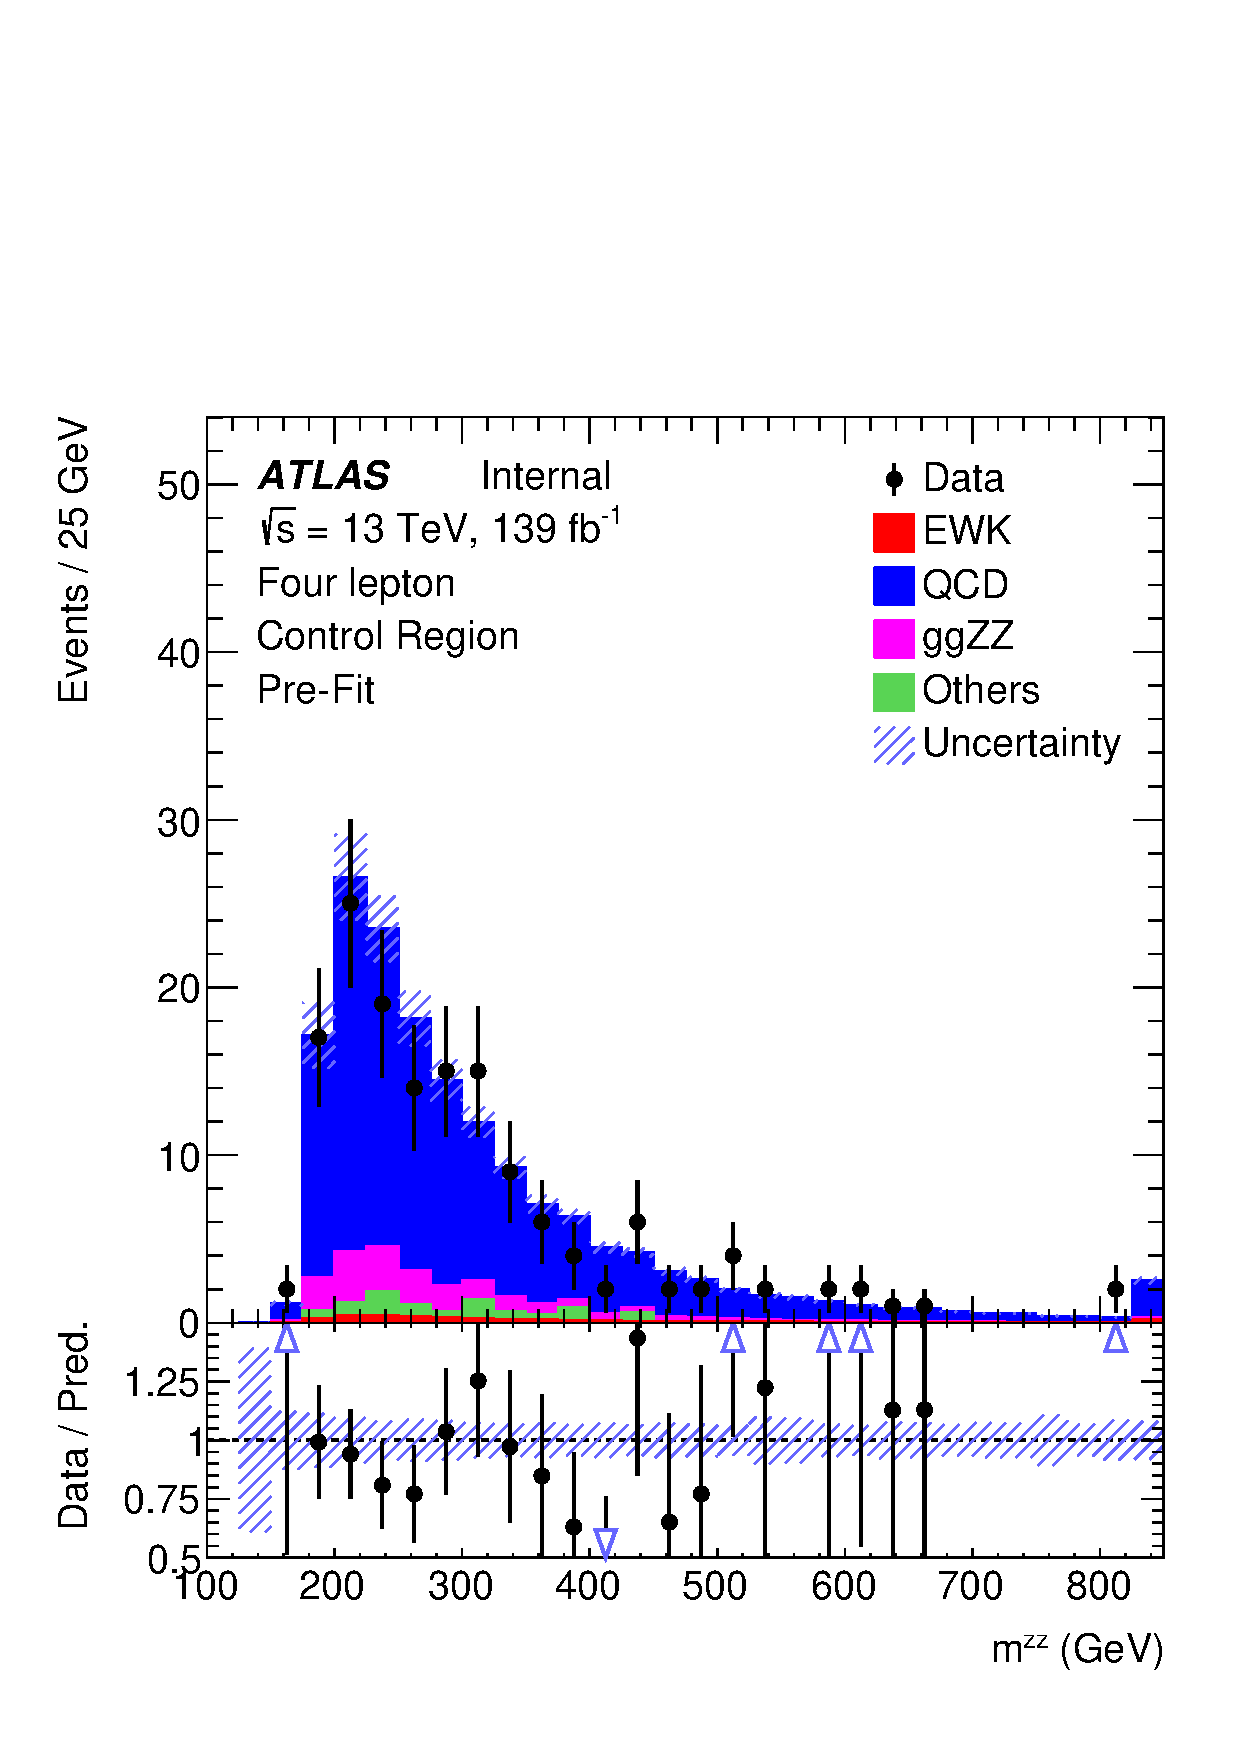
\includegraphics[width=0.42\textwidth]{figures/VBSZZ/QCDCR/MZZ_4l_QCD_CR.pdf}
  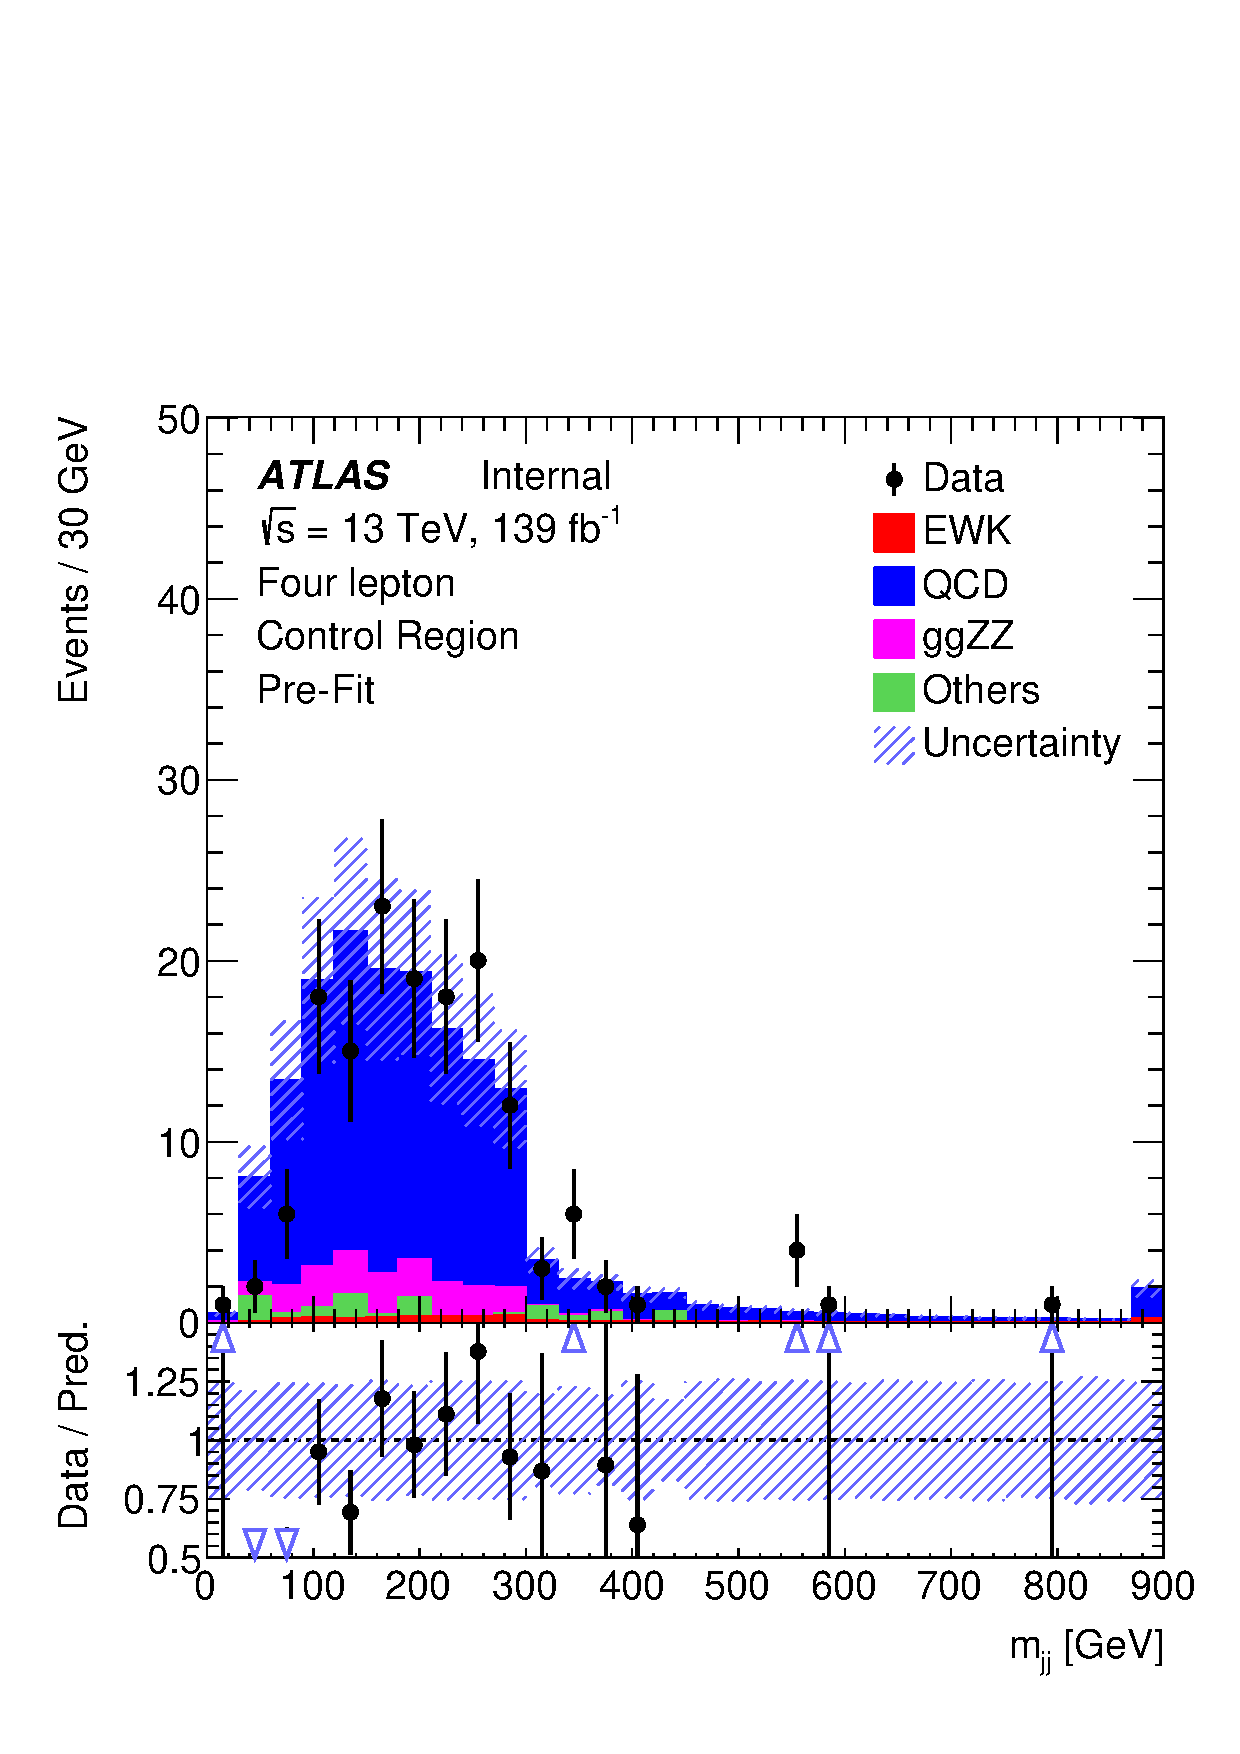
\includegraphics[width=0.42\textwidth]{figures/VBSZZ/QCDCR/MJJ_4l_QCD_CR_fullSyst.pdf}
  \caption{Pre-fit $\mzz$ and $\mjj$ distribution in QCD-enriched CR.}
  \label{fig:qcdcr_prefit}
\end{figure}

\subsection{Fake backgrounds}

Backgrounds from \Zjet, top-quark and $WZ$ processes are estimated by data-driven method.
These events usually contain two or three leptons from Z/W decays, together with heavy-flavor jets or misidentified components of jets reconstructed as leptons called "fake leptons".
A \textit{fake factor} method is used to estimate this backgrounds, in which the lepton misidentification is measured in data regions 
with enhanced contributions from \Zjet and top-quark processes:
\begin{enumerate}
	\item Define a dedicated background dominant region to derive the fake factor for this background. 
The \textit{fake factor} is defined as:
\begin{equation}
	\mathcal{F} = \mathcal{N}_{good} / \mathcal{N}_{pool}
\end{equation}
where $\mathcal{N}_{good}$ refers to the number of good leptons passing all SR selection, while $\mathcal{N}_{pool}$ denotes the number of poor leptons passing most SR selection but fail one certain requirement.
	\item Define a \lllljj fake control region, where one or two leptons pass \textit{poor} requirement while all the other leptons are required to have SR selection.
	\item The number of fake events are calculated as:
\begin{equation}
	\mathcal{N}_{fake} = \left( N_{gggp} - N_{gggp}^{ZZ} \right) \times \mathcal{F} - \left( N_{ggpp} - N_{ggpp}^{ZZ} \right) \times \mathcal{F}^{2}
\end{equation}
with the subtraction of $ZZ$ contribution, and the double counting between ($N_{gggp}$ and $N_{ggpp}$).
\end{enumerate}

For the definition of \textit{poor} leptons:
The poor electrons are defined as failing "FixedCutLoose" isolation requirement or "LooseLH" electron ID requirement but satisfying "VeryLooseLH" WP.
The poor muons are required to fail the "FixedCutLoose" isolation requirement or invert the impact parameter cut to be $3 < d_{0}/\sigma(d_{0}) < 10$.
The dedicated \Zjet and \ttbar dominant regions are defined to calculate the fake factor respectively in the following subsections.
%For other minor fake contributions like $WZ$, $W + jets$ and $W^{+}W^{-} + jets$ without additional dedicated CR, the estimations are included into 

\subsubsection{Fake factor for \Zjet}

Fake factor for \Zjet background is calculated in \Zjet-enriched region, where events with one SFOS lepton pair around $Z$ mass associated with two jets are selected.
The value of fake factor is driven from data, and as a function of $p_{T}$ and $\eta$ as shown in figure~\ref{fig:fake_zjet_el} for electrons and figure~\ref{fig:fake_zjet_mu} for muons.
During calculation, the contributions from non-\Zjet backgrounds (\ttbar, $ZZ$, $WZ$) have been subtracted from data.
The values calculated from \Zjet MC directly are also shown in plots for comparison.
\begin{figure}[!htb]
  \centering
  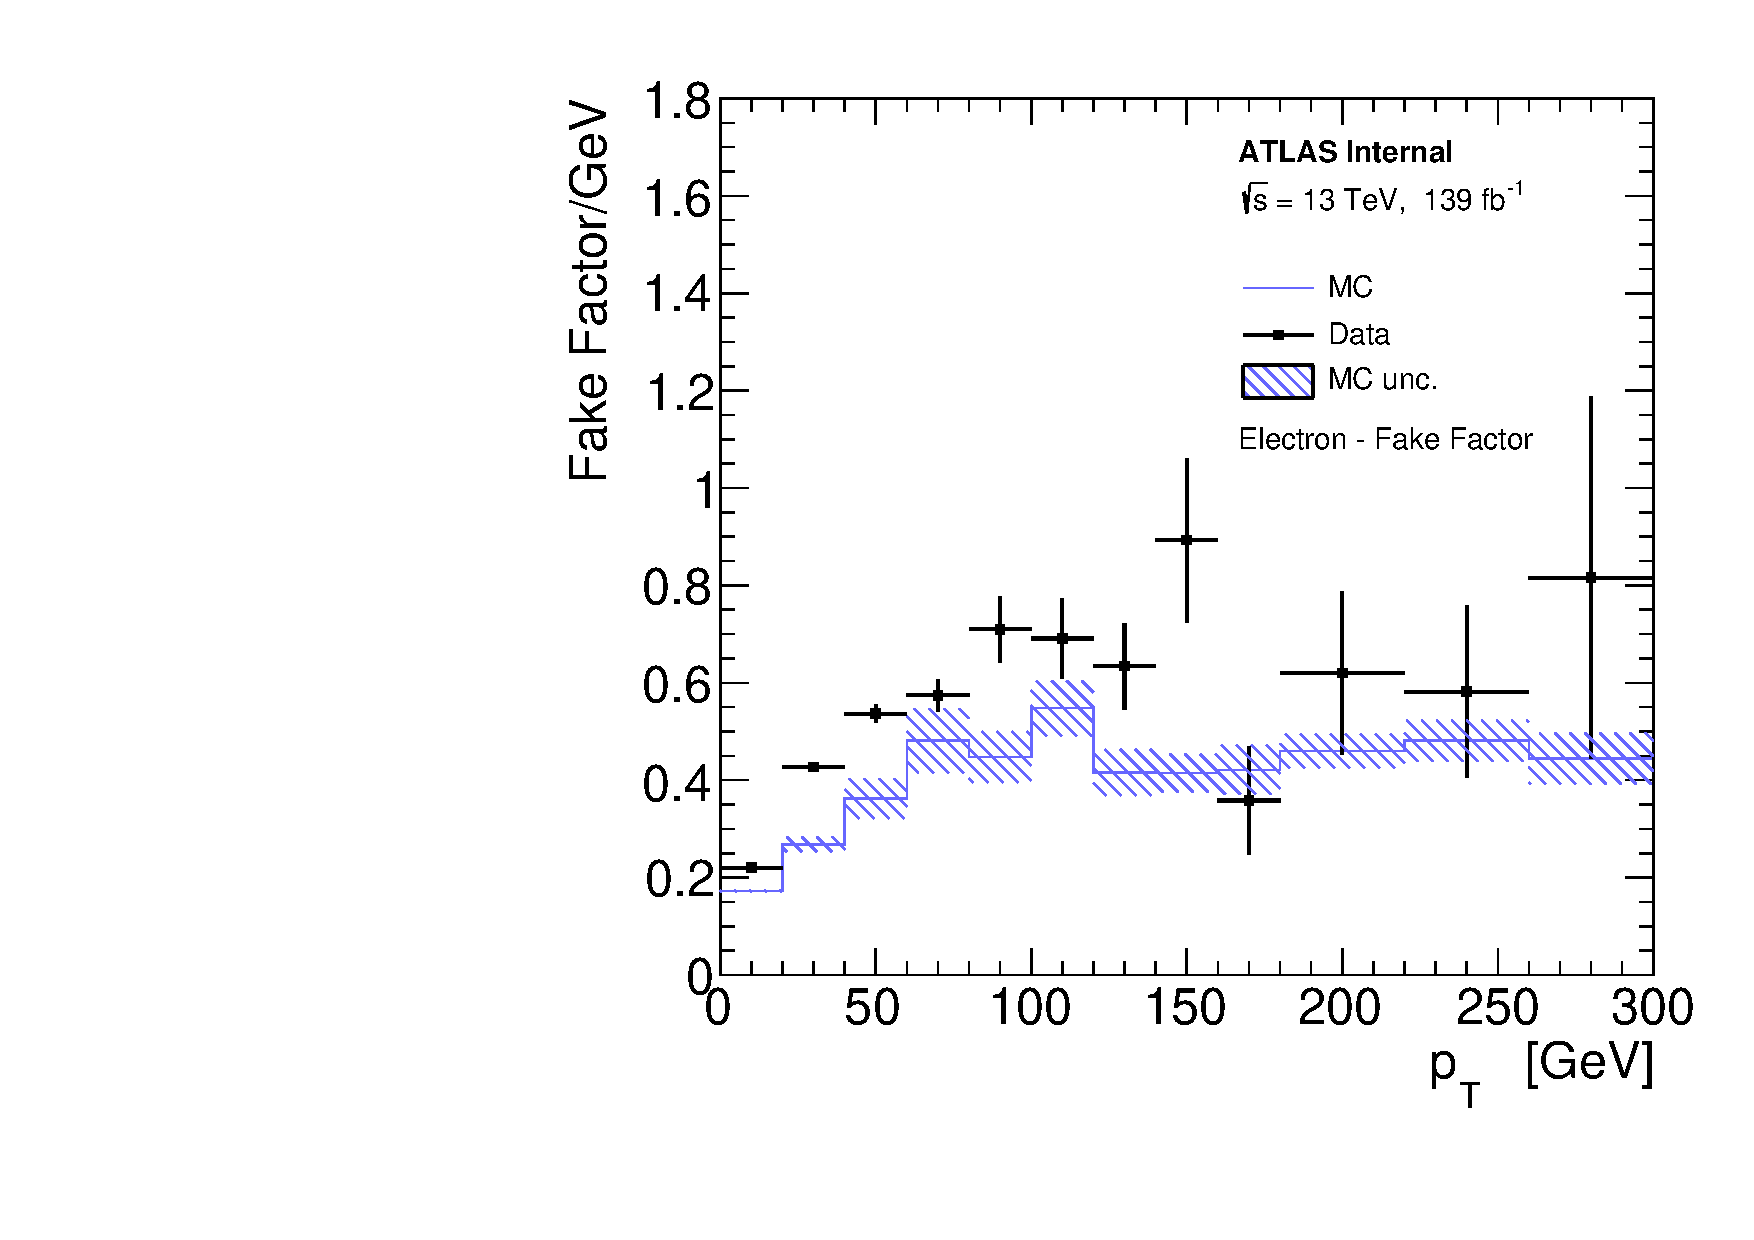
\includegraphics[width=0.42\textwidth]{figures/VBSZZ/fakebkg/Electron_2Dff_ptfakeFactorAddElectron_etapt_pavgy.pdf}
  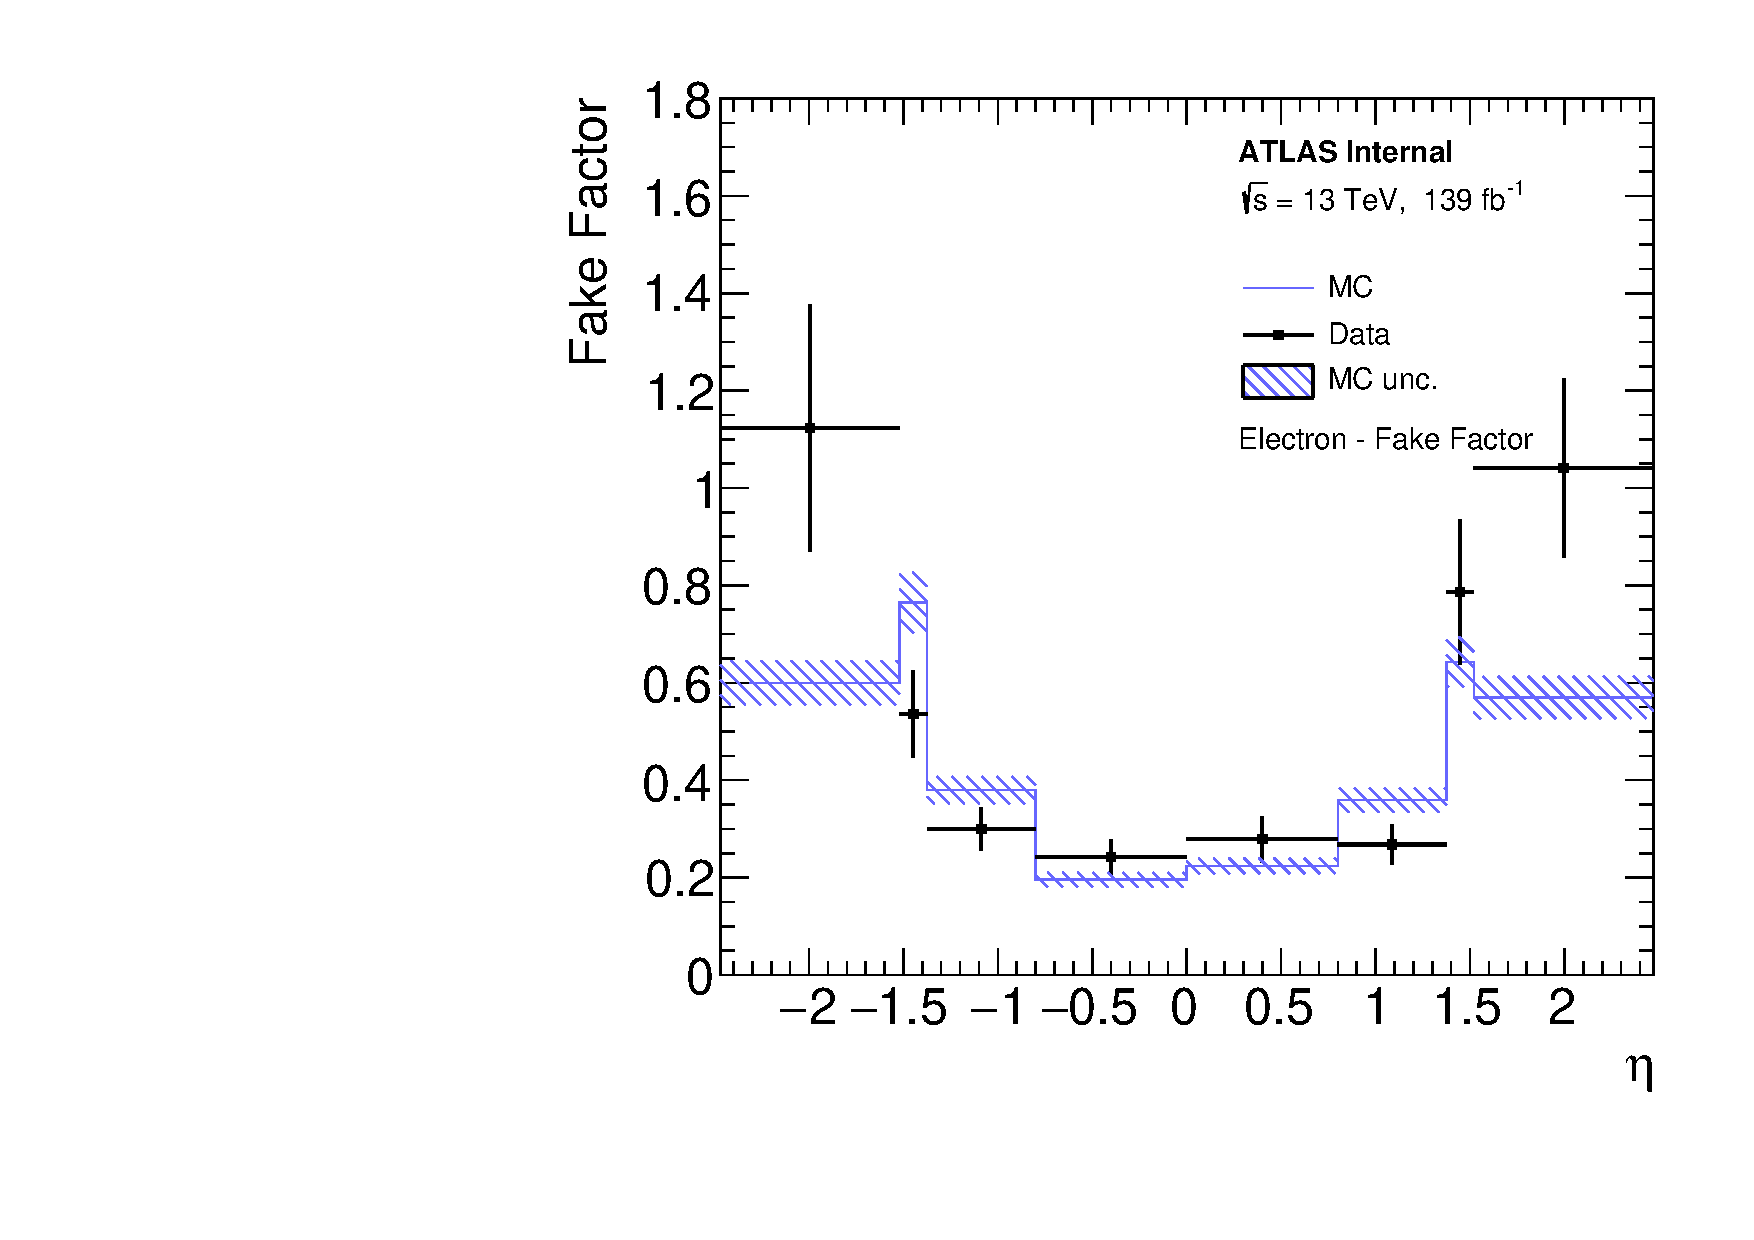
\includegraphics[width=0.42\textwidth]{figures/VBSZZ/fakebkg/Electron_2Dff_etafakeFactorAddElectron_etapt_pavgx.pdf}
  \caption{Fake factor for $\Zjet$ background, constructed with additional electron, as a function of $p_{T}$ (left) and $\eta$ (right).}
  \label{fig:fake_zjet_el}
\end{figure}

\begin{figure}[!htb]
  \centering
  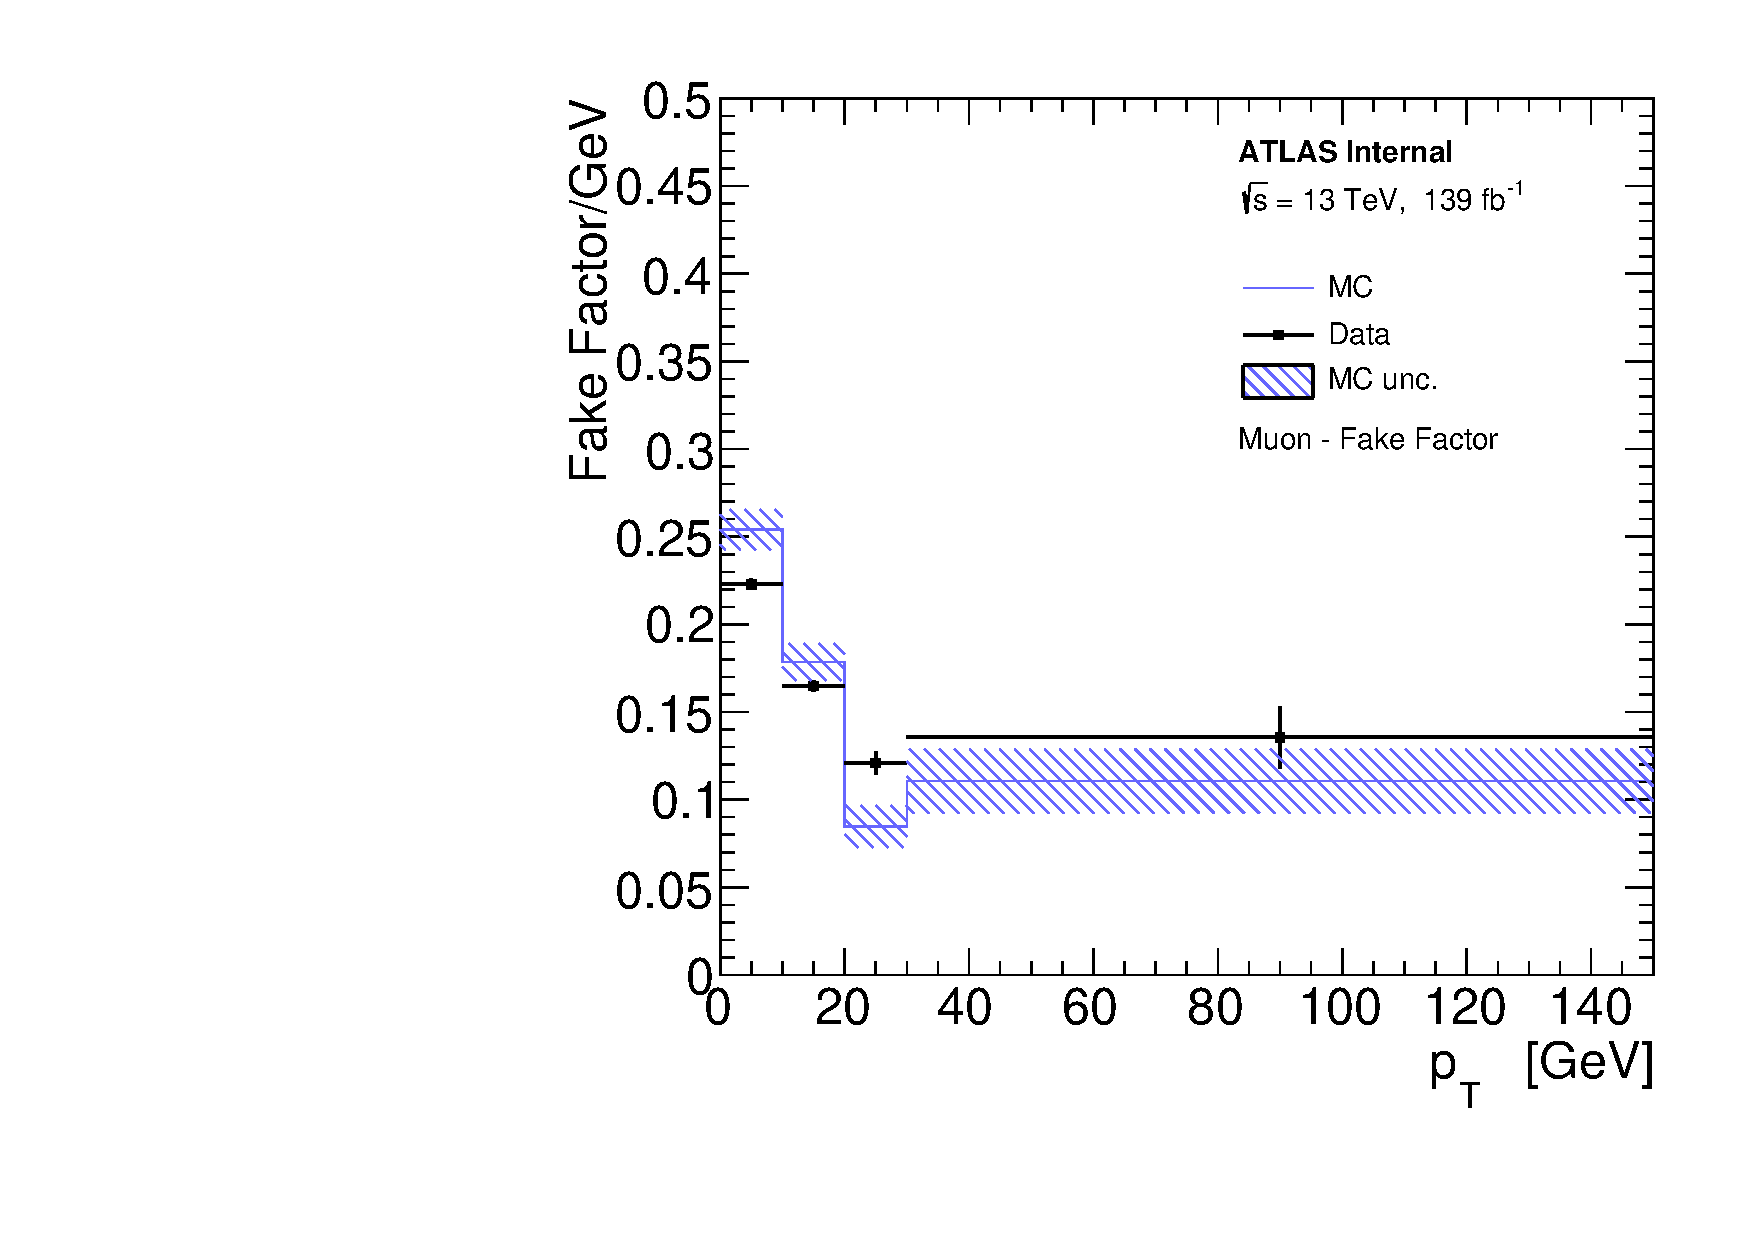
\includegraphics[width=0.42\textwidth]{figures/VBSZZ/fakebkg/Muon_2Dff_ptfakeFactorAddMuon_etapt_pavgy.pdf}
  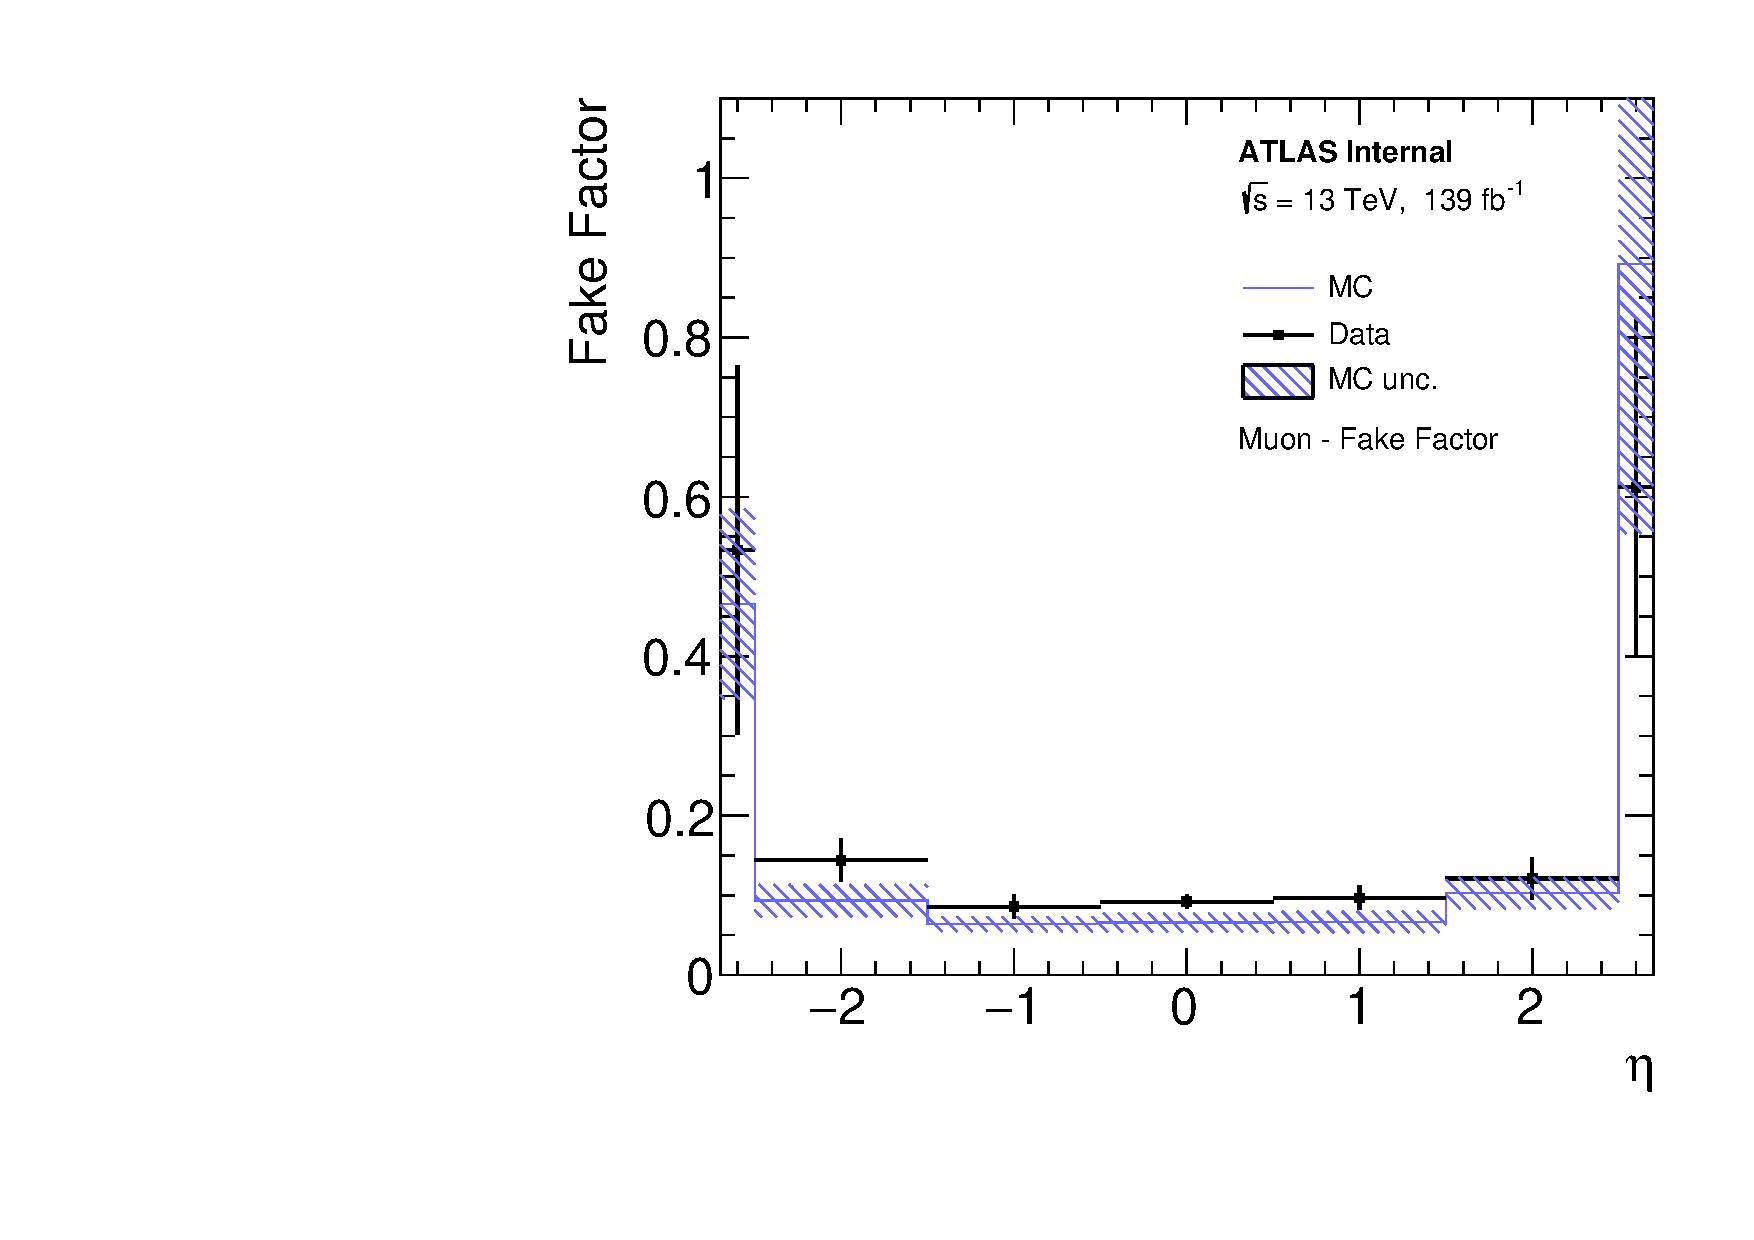
\includegraphics[width=0.42\textwidth]{figures/VBSZZ/fakebkg/Muon_2Dff_etafakeFactorAddMuon_etapt_pavgx.pdf}
  \caption{Fake factor for $\Zjet$ background, constructed with additional muon, as a function of $p_{T}$ (left) and $\eta$ (right).}
  \label{fig:fake_zjet_mu}
\end{figure}

\subsubsection{Fake factor for \ttbar}

The fake factor for \ttbar are calculated in \ttbar dominanted region by selecting one $e\mu$-pair with additional two jets.
For events with three leptons, $m_{T}^{W} <$ 60~\gev cut is applied to reject the constribution from \ttbar + W events.
The $m_{T}^{W}$ is defined as below:
\begin{equation}
	m_{T}^{W} = \sqrt{ 2p_{T}^{l_{3}} E_{T}^{miss} \left[1-cos\left(\Delta\phi\left(p_{T}^{l_{3}}, E_{T}^{miss}\right)\right)\right] }
\end{equation}
In addition, at least one b-jet is required to enhance the top component.
The fake factors of \ttbar calculated from data as the function of $p_{T}$ and $\eta$ are shown in figure~\ref{fig:fake_tt_el} for electrons and ~\ref{fig:fake_tt_mu} for muons.
The non-\ttbar contributions, which include \Zjet, $ZZ$ and $WZ$, are subtracted from data.
\begin{figure}[!htb]
  \centering
  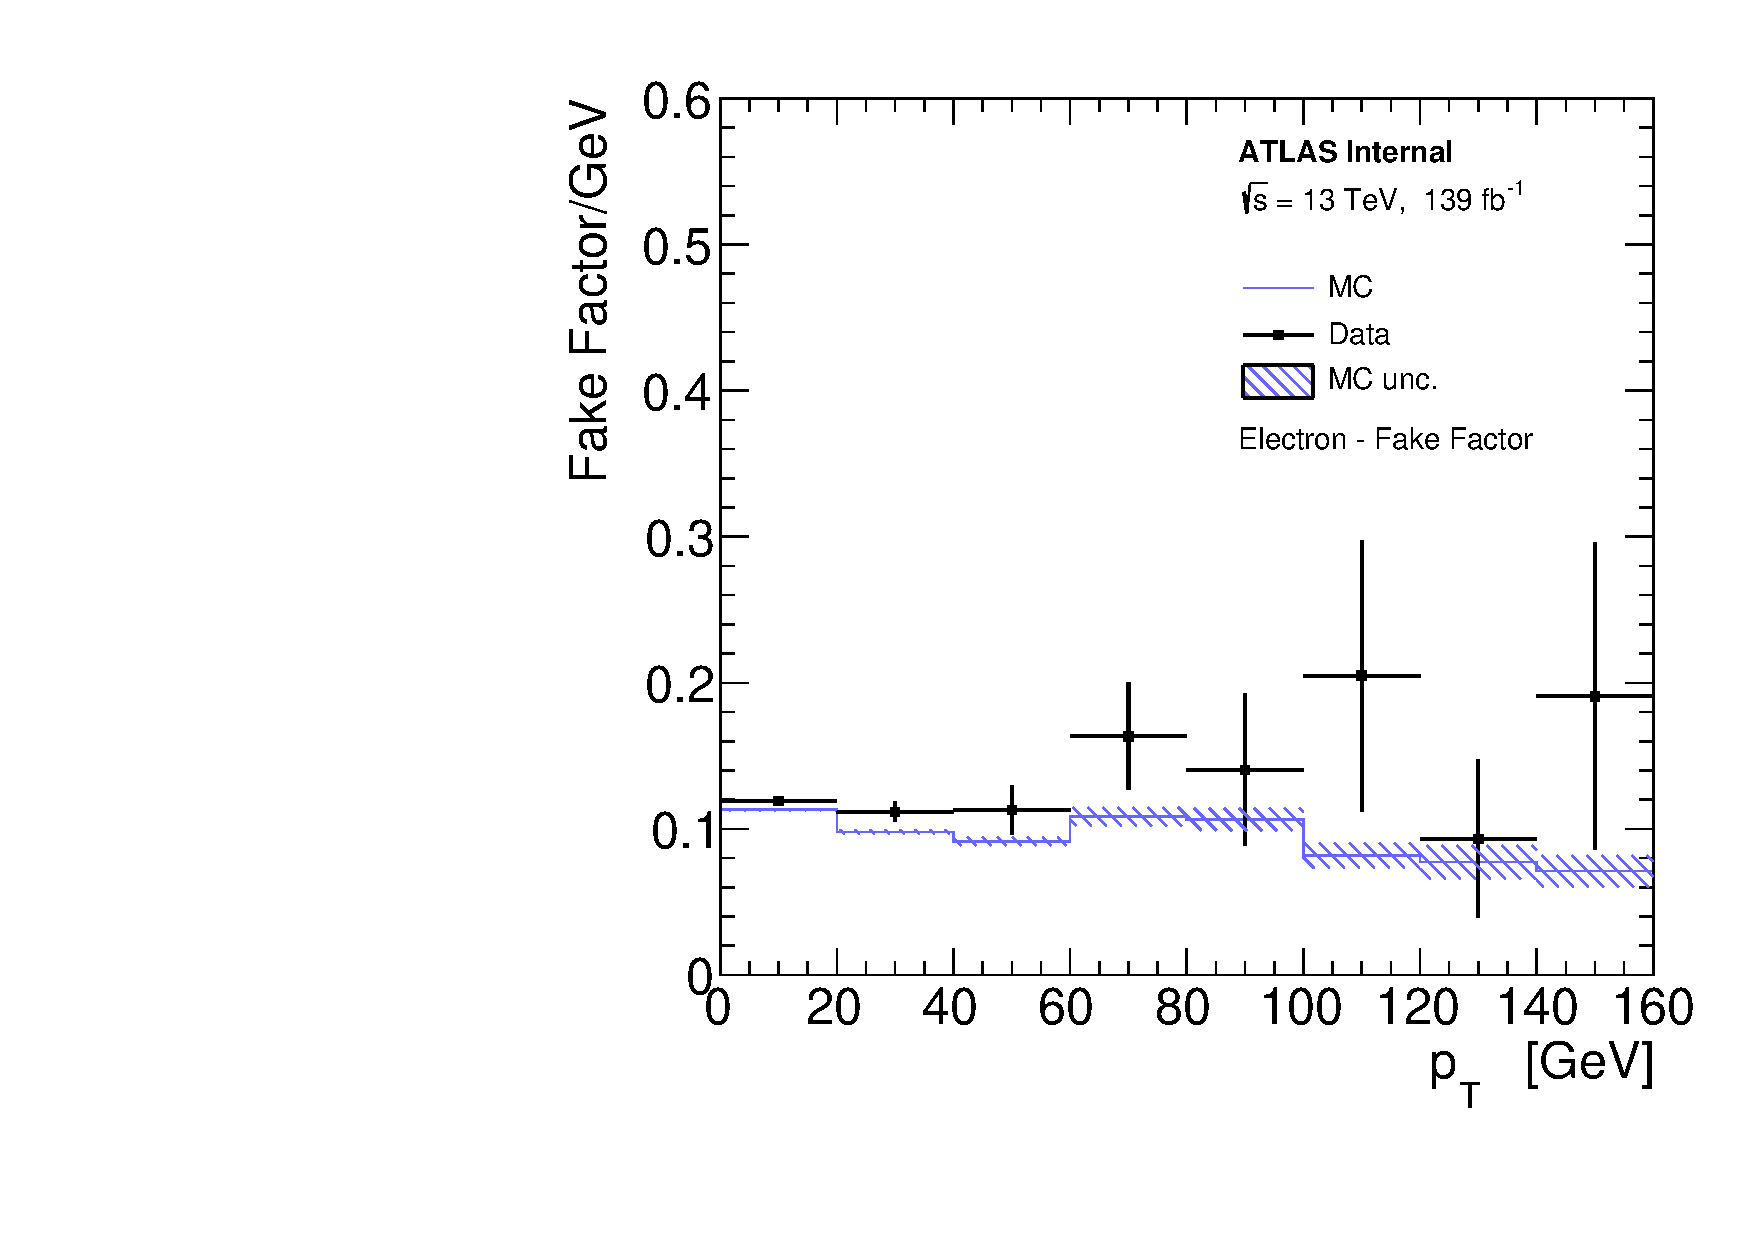
\includegraphics[width=0.42\textwidth]{figures/VBSZZ/fakebkg/Electron_2Dff_ptttbarFakeFactorAddElectron_etapt_pavgy.pdf}
  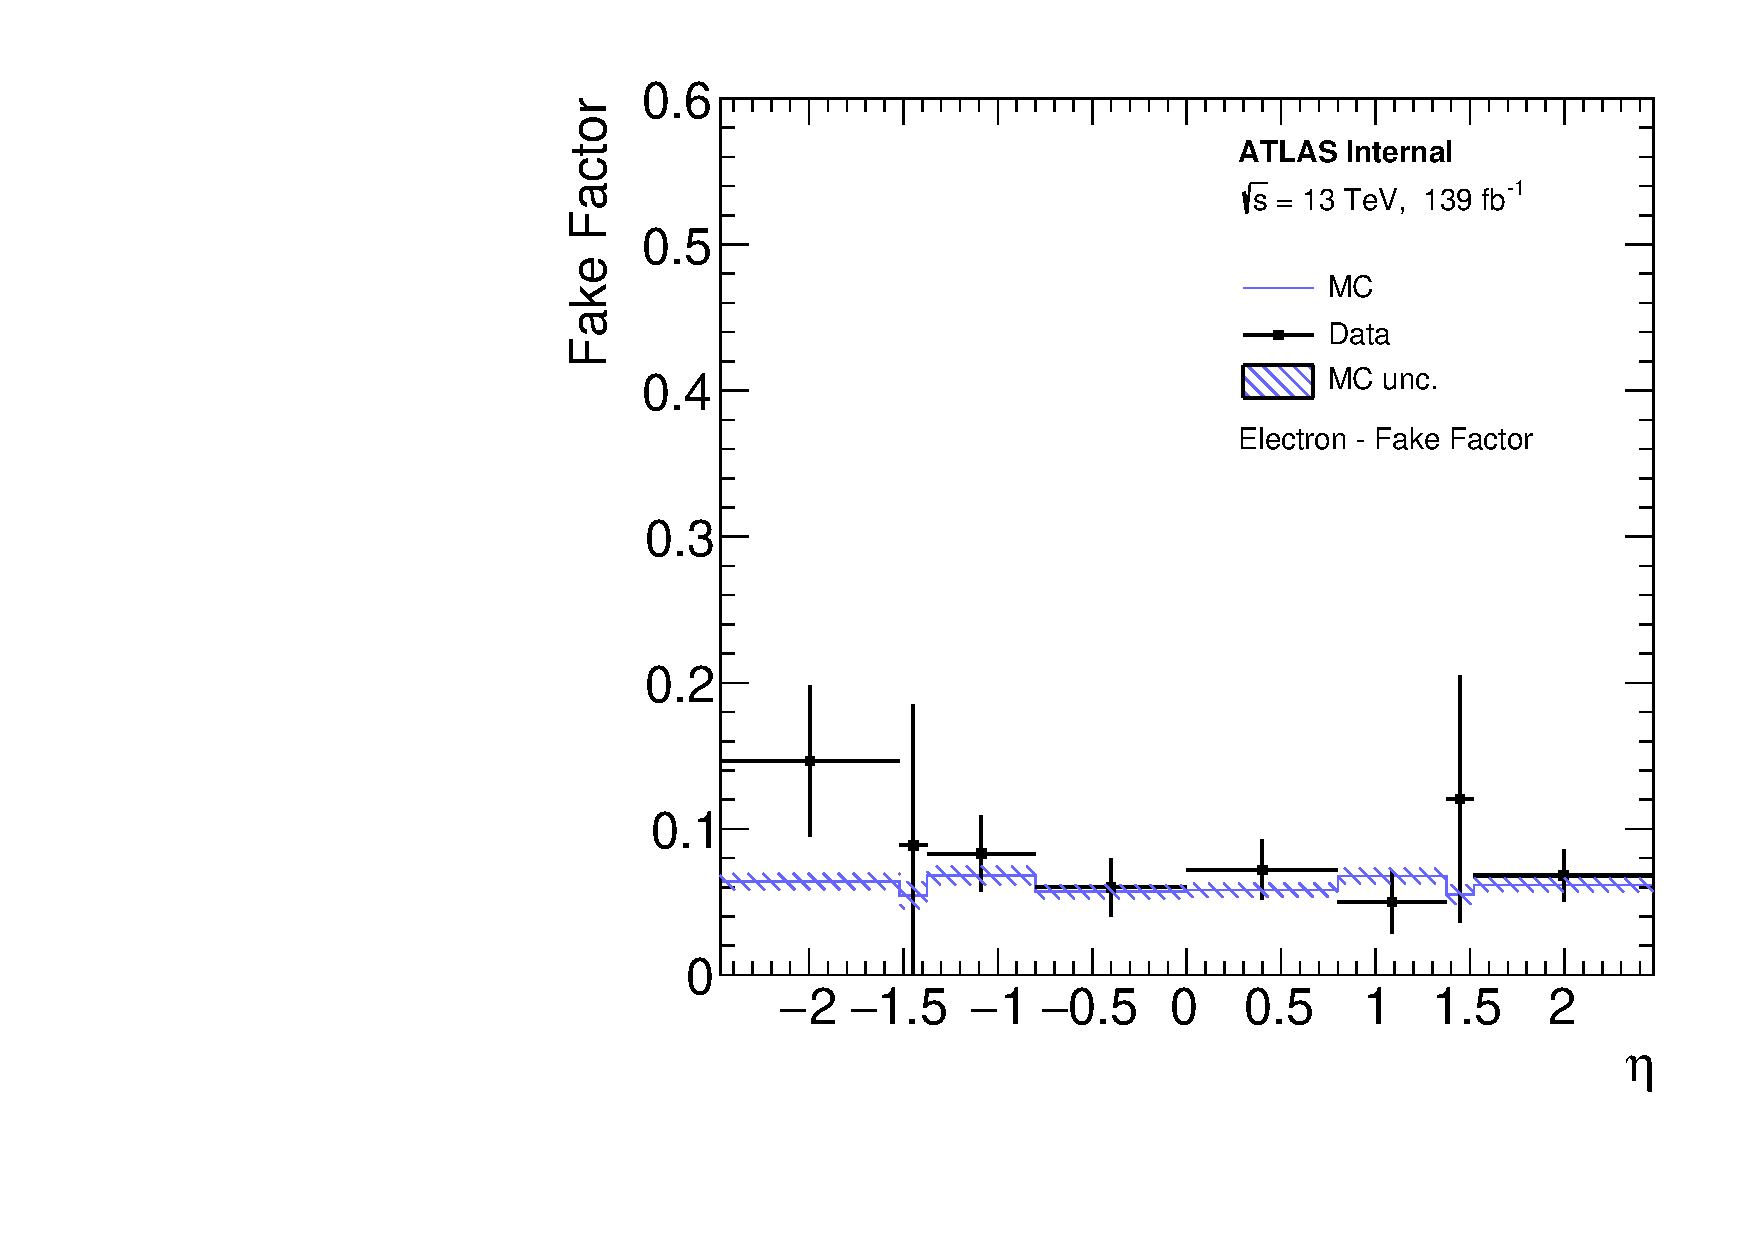
\includegraphics[width=0.42\textwidth]{figures/VBSZZ/fakebkg/Electron_2Dff_etattbarFakeFactorAddElectron_etapt_pavgx.pdf}
  \caption{Fake factor for $\ttbar$ background, constructed with additional electron, as a function of $p_{T}$ (left) and $\eta$ (right).}
  \label{fig:fake_tt_el}
\end{figure}

\begin{figure}[!htb]
  \centering
  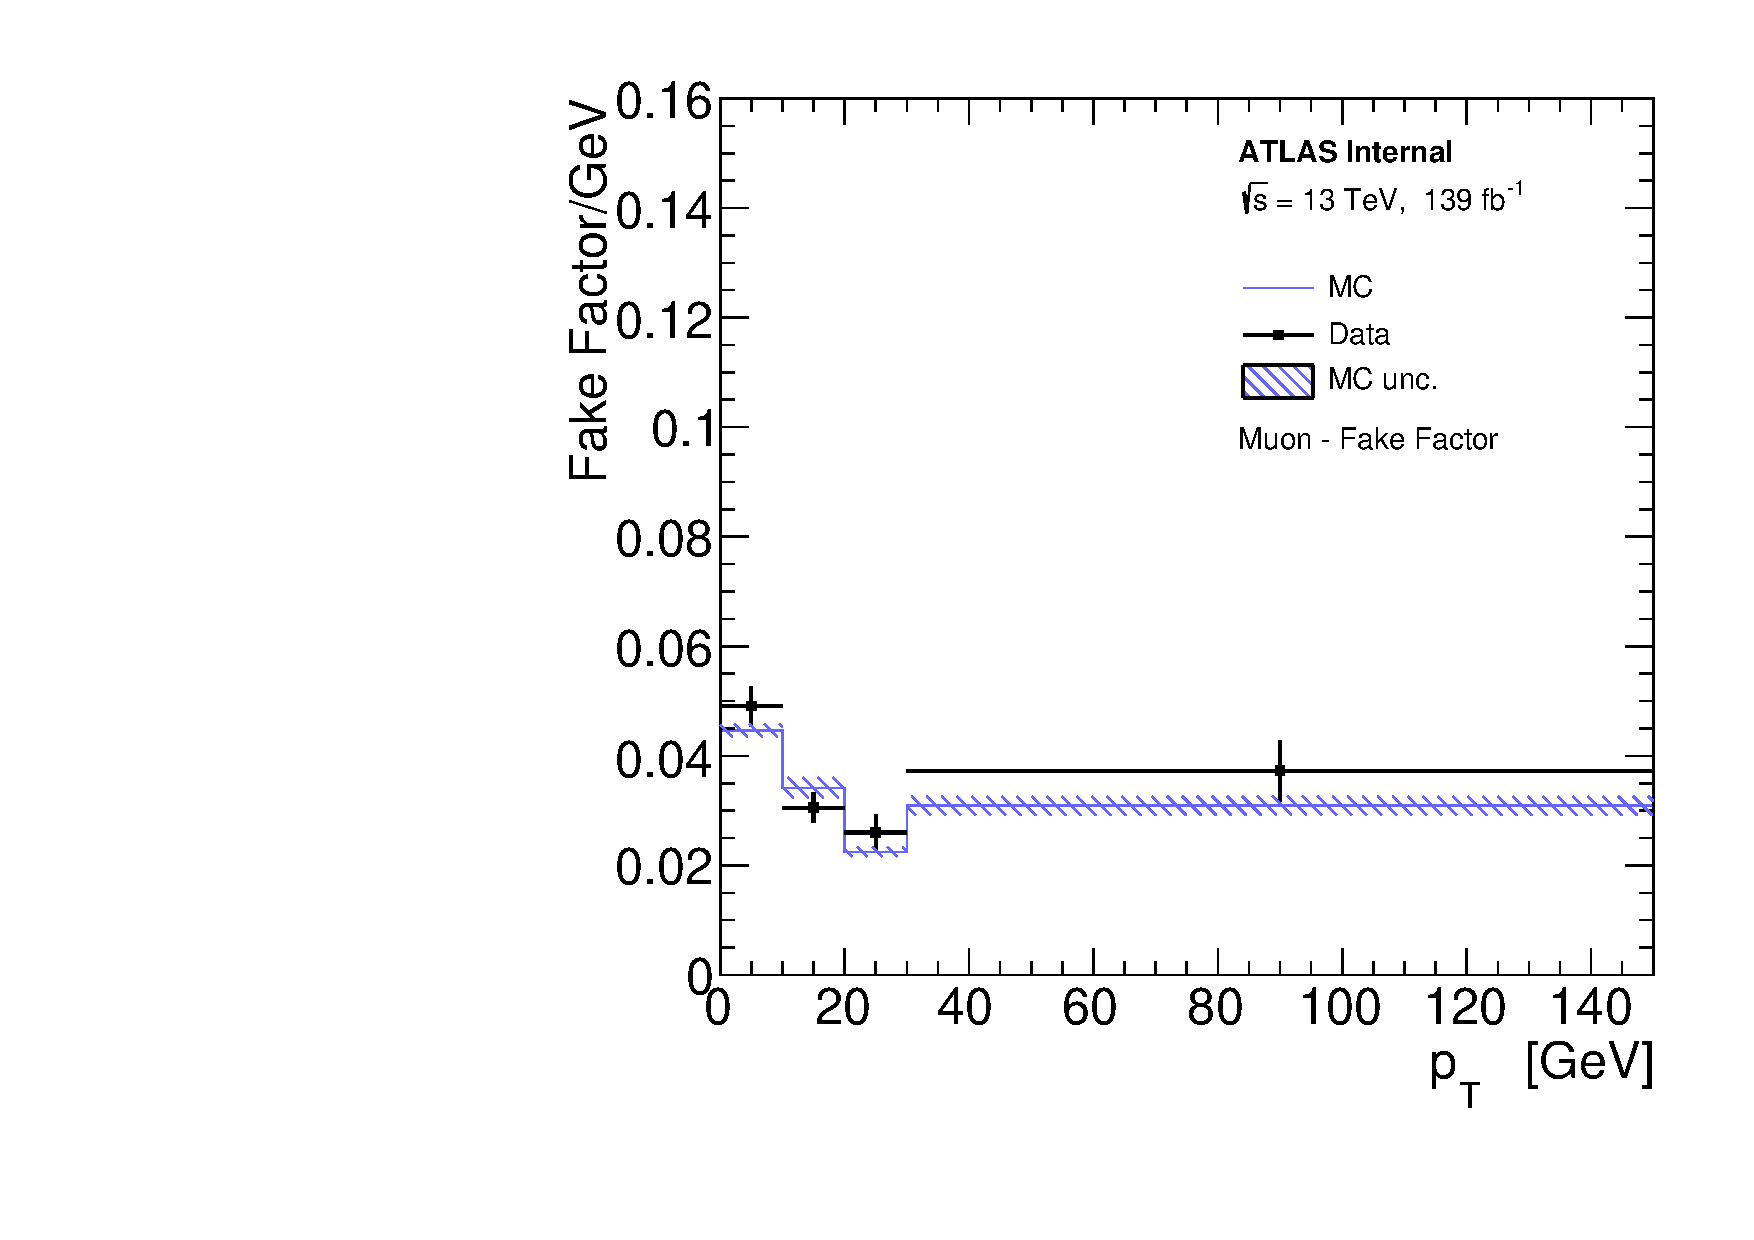
\includegraphics[width=0.42\textwidth]{figures/VBSZZ/fakebkg/Muon_2Dff_ptttbarFakeFactorAddMuon_etapt_pavgy.pdf}
  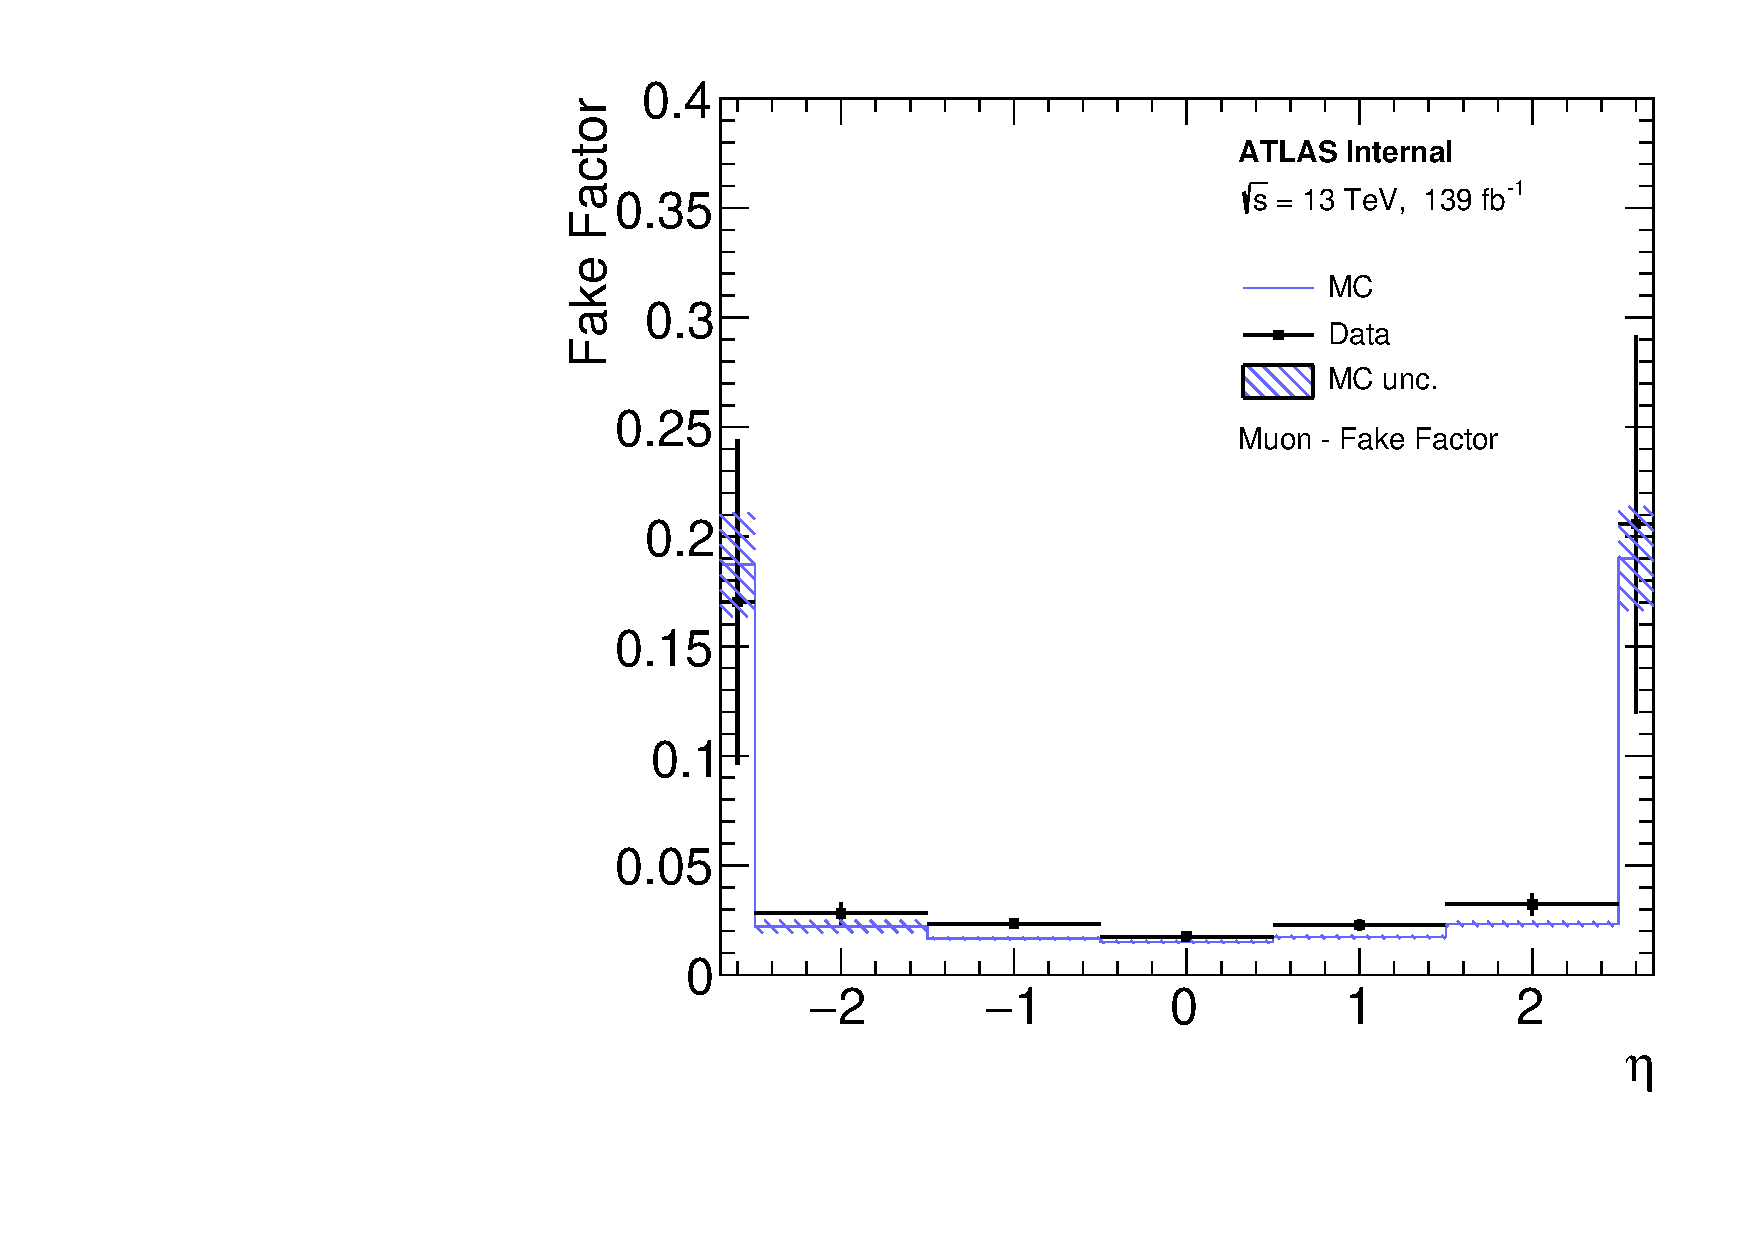
\includegraphics[width=0.42\textwidth]{figures/VBSZZ/fakebkg/Muon_2Dff_etattbarFakeFactorAddMuon_etapt_pavgx.pdf}
  \caption{Fake factor for $\ttbar$ background, constructed with additional muon, as a function of $p_{T}$ (left) and $\eta$ (right).}
  \label{fig:fake_tt_mu}
\end{figure}

\subsubsection{Combination}

The fake factors calculated from each dedicated region are then combined together according to their contributions in fake control region described previously.
Figure~\ref{fig:fake_mjj} shows the \mjj distribution with data and major fake backgrounds in three different 4l channels.
\begin{figure}[!htb]
  \centering
  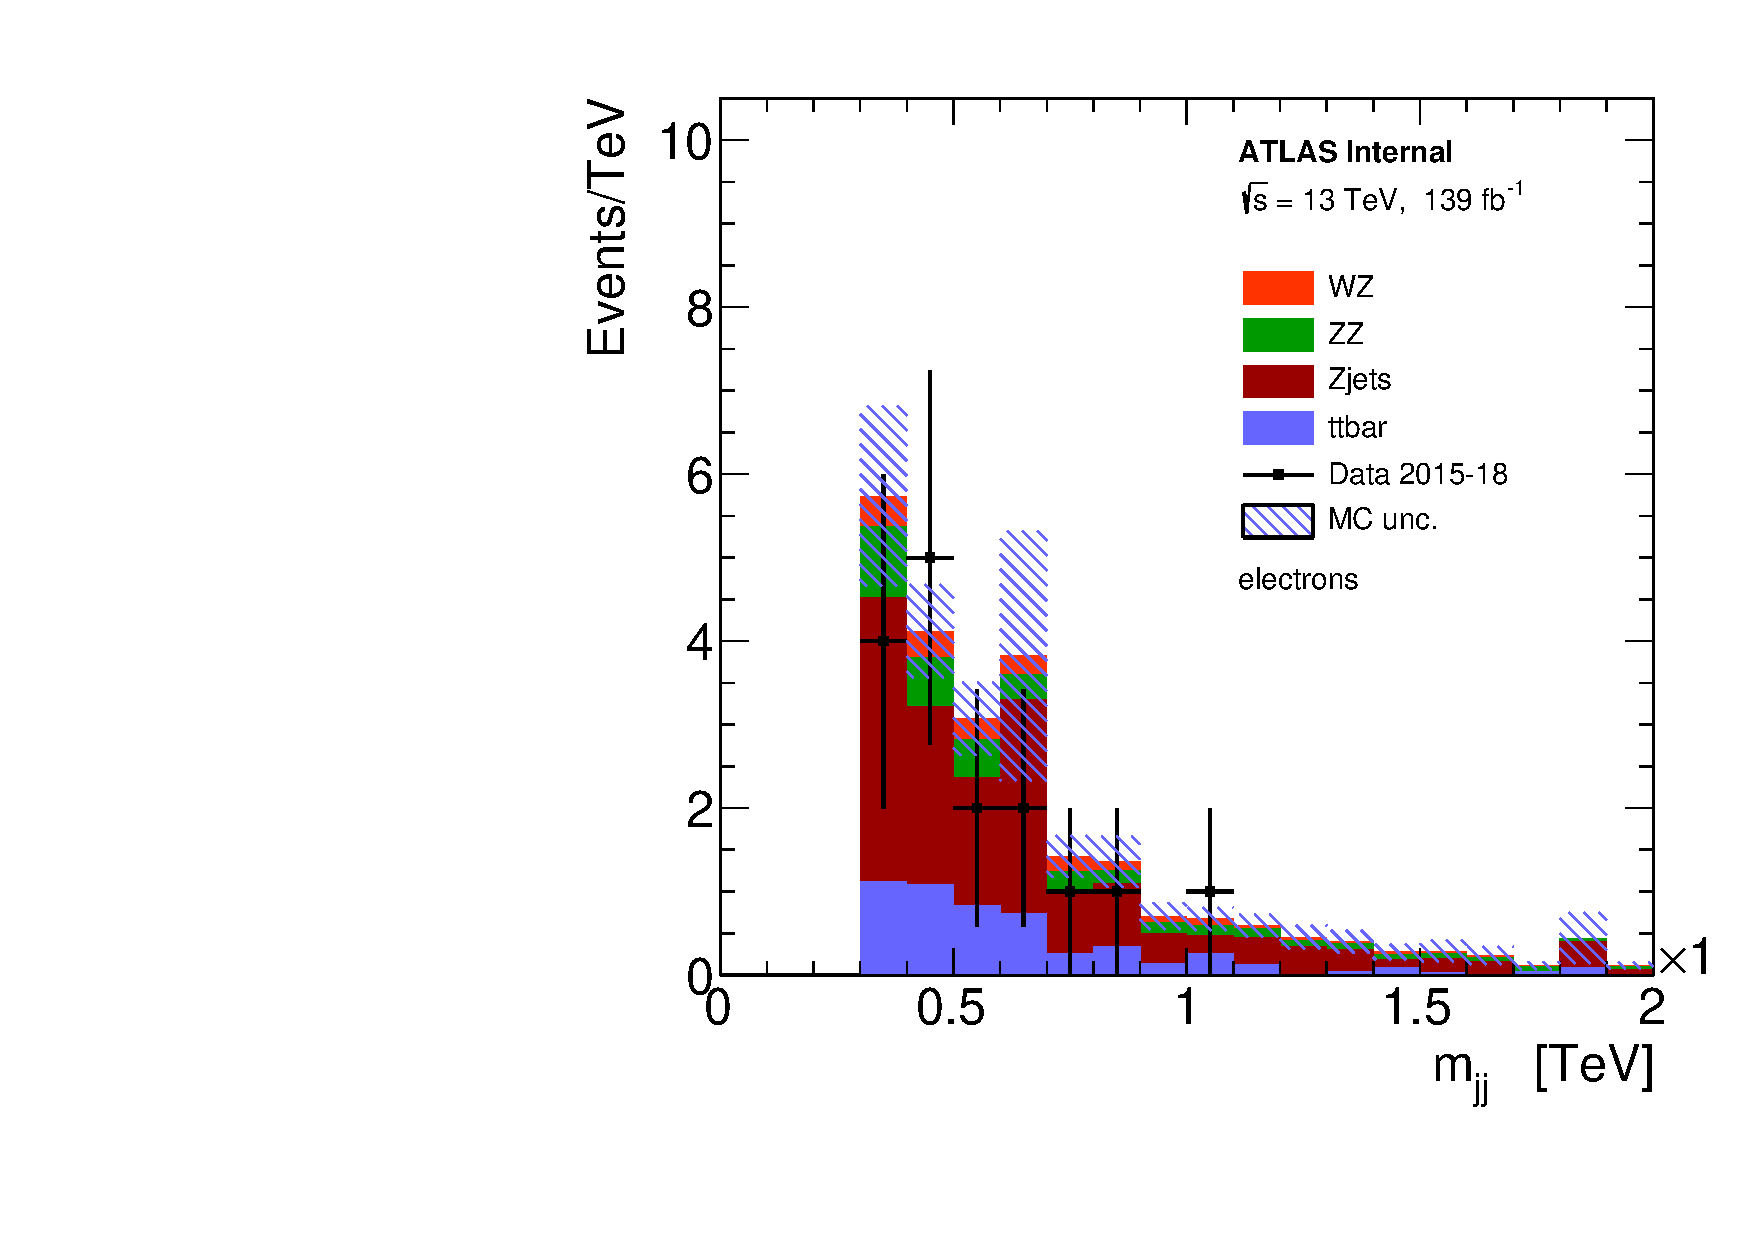
\includegraphics[width=0.32\textwidth]{figures/VBSZZ/fakebkg/15161718_mva_dijet_mass_zjet_ttbar_ratio_electrons_mva_dijet_mass.pdf}
  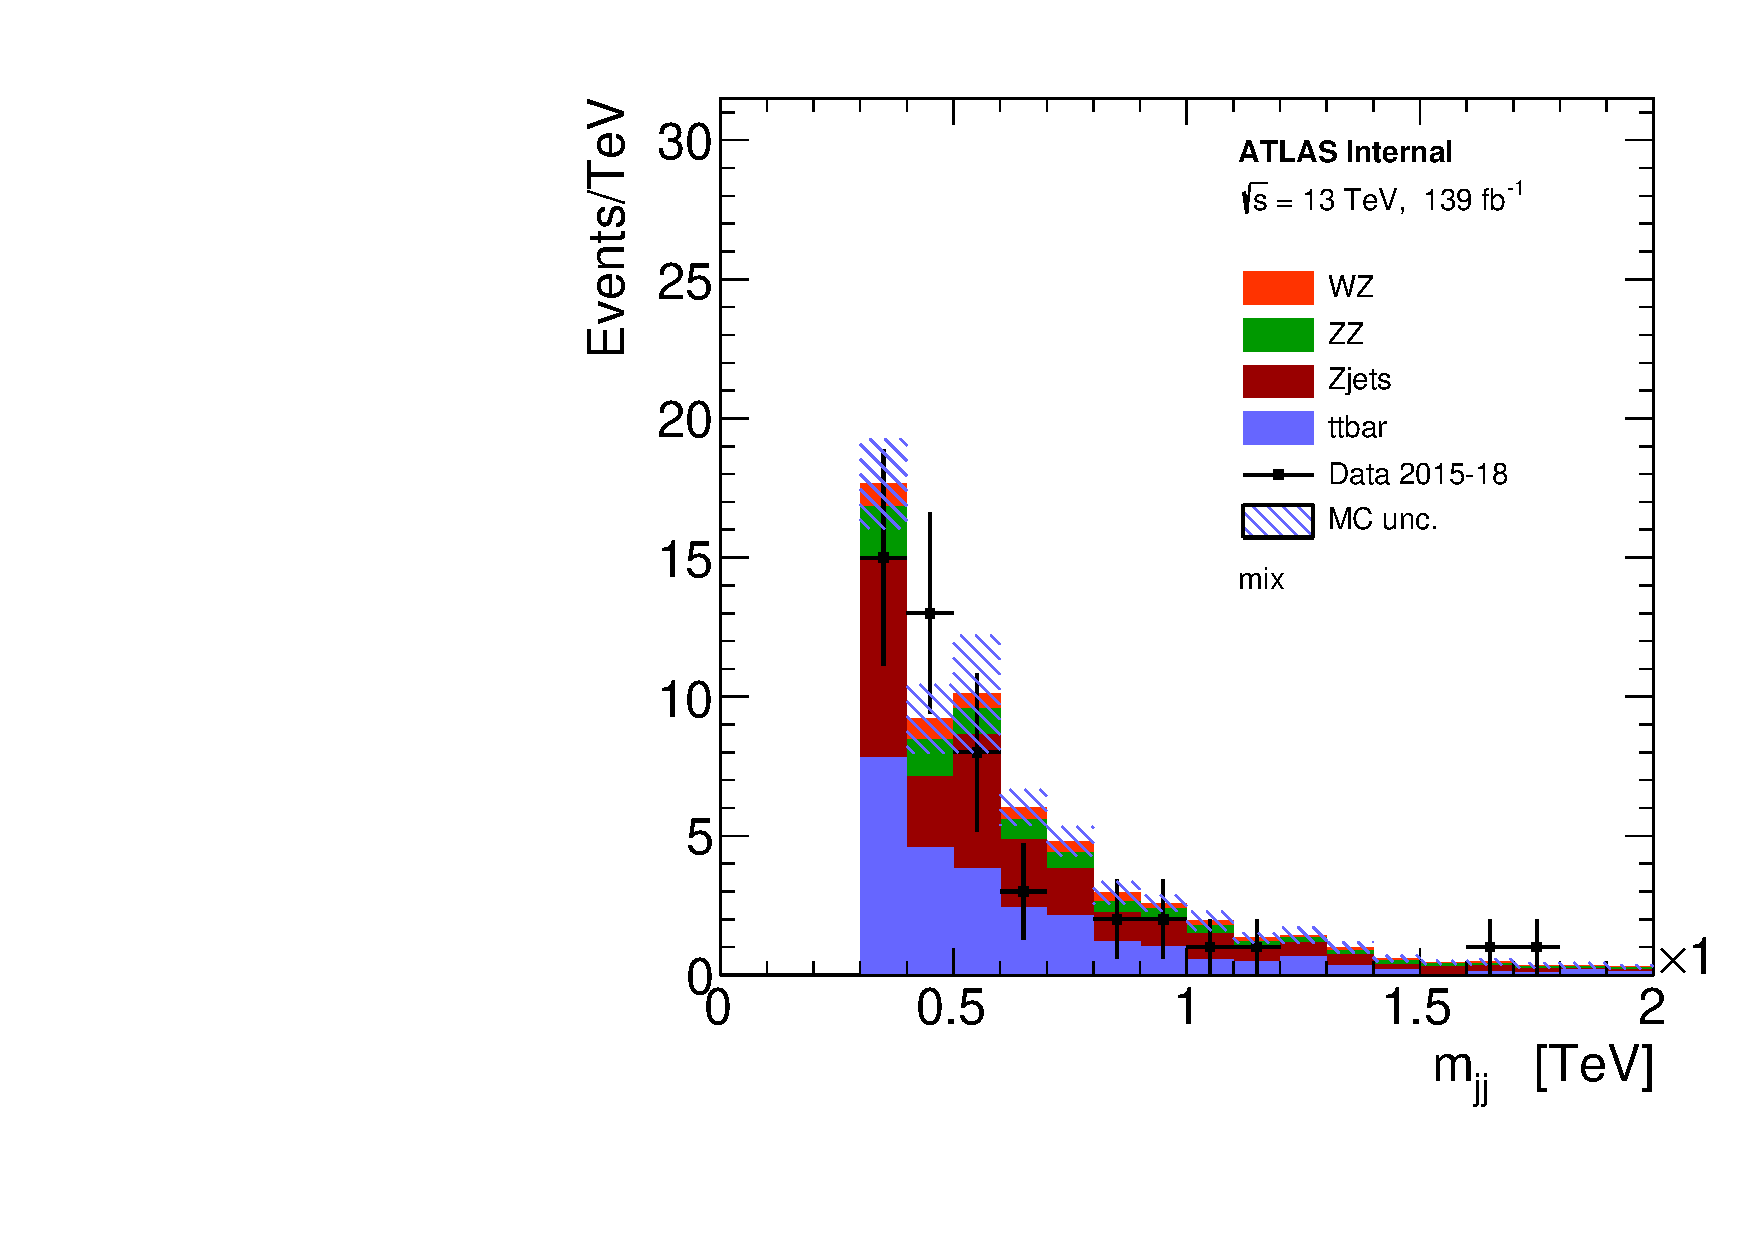
\includegraphics[width=0.32\textwidth]{figures/VBSZZ/fakebkg/15161718_mva_dijet_mass_zjet_ttbar_ratio_mix_mva_dijet_mass.pdf}
  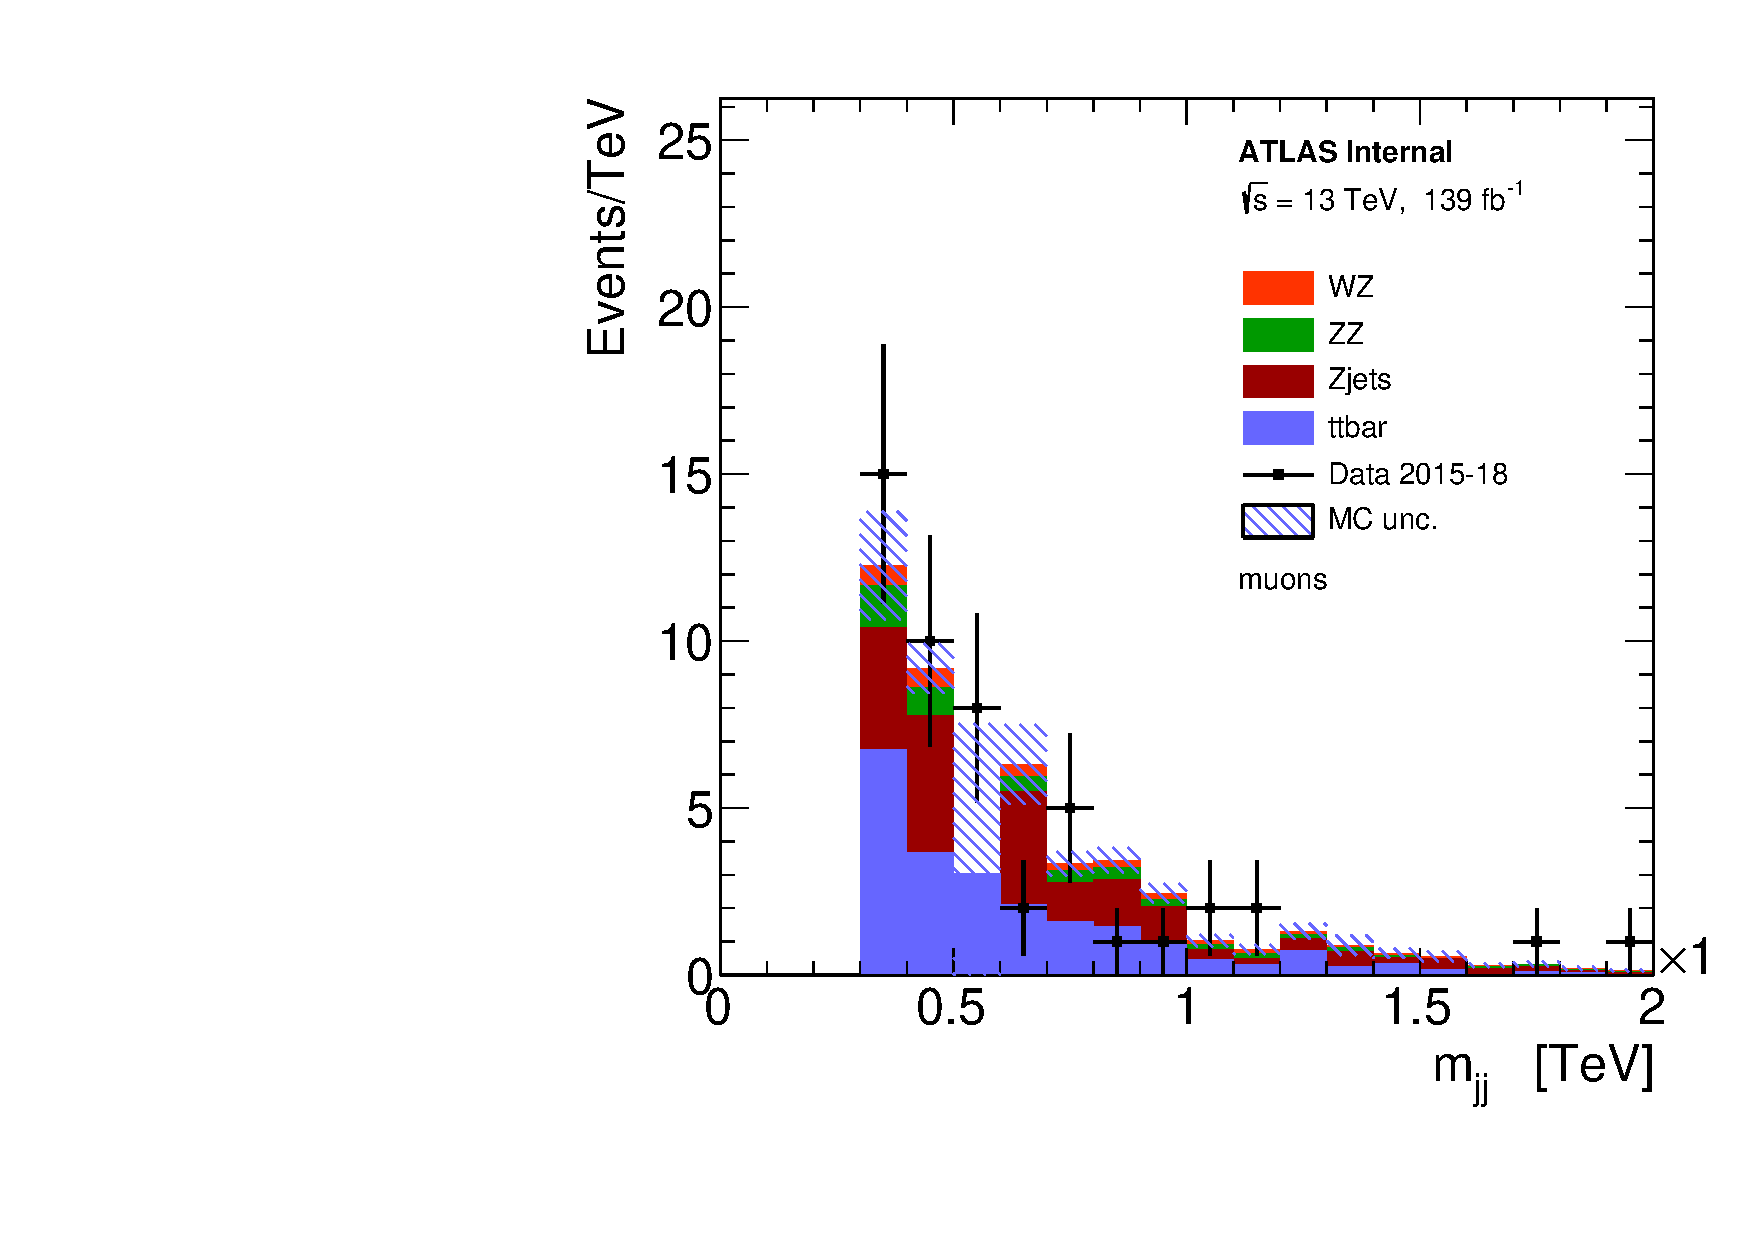
\includegraphics[width=0.32\textwidth]{figures/VBSZZ/fakebkg/15161718_mva_dijet_mass_zjet_ttbar_ratio_muons_mva_dijet_mass.pdf}
  \caption{$\mjj$ distributions in fake control region in 4e (left), 2e2$\mu$ (middle) and 4$\mu$ (right) channel.
The ratios between $\Zjet$ and $\ttbar$ ($\Zjet / \ttbar$) in each individual channel are: 2.59, 0.95, 0.74.}
  \label{fig:fake_mjj}
\end{figure}

\subsubsection{Systematics of fake estimation and results}
\label{sec:fake_syst}

The systematics of fake factor method can be measured by varying the parameters and selection requirements in fake factor calculation.
In addition, due to the very limited data statistic in \llll channel, to be more conservative, 
the difference between data measurement and MC simulation are also considered as another systematics component.
In detail, the sources of systematics that have been included are listed as below:
\begin{itemize}
	\item Variations of isolation cut for the poor lepton definition up and down scaled by a factor of two.
	\item Variations of the yields of those subtracted MC in fake control region scaled by 30\% up and down.
	\item The difference of fake factors between driven from data and from MC simulation.
	\item The difference of fake factors when changing to one bin measurement (instead of $p_{T}$ or $\eta$ dependent).
	\item The statistical uncertainties on fake factor in fake control region.
\end{itemize}

Table~\ref{tab:fake_uncer} summarizes the contribution of fake backgrounds in signal region under different systematic conditions mentioned above as well as the nominal one.
Uncertainties of each value in table are statistical one.
\begin{table}[h]
    \centering
    \resizebox{1.0\columnwidth}{!}{
        \begin{tabular}{lrrrr}
        channel & 4e &   2e2$\mu$ &    4$\mu$ &   inclusive \\ 
	\hline
        Nominal estimate                  & 0.678$\pm$ 0.652 & 1.023$\pm$ 0.740 & 0.566$\pm$ 0.240 & 2.268$\pm$ 1.015 \\
        $F$ stat. uncertainty varied down & 0.698$\pm$ 0.622 & 0.872$\pm$ 0.652 & 0.509$\pm$ 0.214 & 2.079$\pm$ 0.926 \\
        $F$ stat. uncertainty varied up   & 0.657$\pm$ 0.685 & 1.173$\pm$ 0.840 & 0.622$\pm$ 0.267 & 2.452$\pm$ 1.116 \\
        One bin $F$                       & 0.653$\pm$ 0.590 & 0.594$\pm$ 0.558 & 0.646$\pm$ 0.313 & 1.892$\pm$ 0.870 \\
        MC $F$                            & 0.534$\pm$ 0.471 & 1.415$\pm$ 0.993 & 0.439$\pm$ 0.184 & 2.389$\pm$ 1.114 \\
        Isolation varied down             & 0.938$\pm$ 0.686 & 0.552$\pm$ 0.466 & 0.215$\pm$ 0.107 & 1.704$\pm$ 0.837 \\
        Isolation varied up               & 0.723$\pm$ 0.646 & 1.104$\pm$ 0.739 & 0.559$\pm$ 0.237 & 2.386$\pm$ 1.010 \\
        MC corr. varied down              & 0.697$\pm$ 0.695 & 1.048$\pm$ 0.811 & 0.832$\pm$ 0.385 & 2.577$\pm$ 1.136 \\
        MC corr. varied up                & 0.660$\pm$ 0.614 & 0.984$\pm$ 0.687 & 0.316$\pm$ 0.159 & 1.961$\pm$ 0.935 \\
        \hline
        \end{tabular}
        }
    \caption{
    Fake background estimations in the SR. For the nominal value the 2D fake factor together with the \Zjet and \ttbar combination applied.
    The other lines show the estimations with different uncertainty variations.
    }
    \label{tab:fake_uncer}
\end{table}


\section{Systematics}
\label{sec:systematics}

The analysis performances both the statistical fit to MD distribution to extract the EW-$ZZjj$ contributions
and the cross section measurements in fiducial volume.
Therefore, theoretical and experimental uncertainties may affect the predictions background yields and shapes, 
correction factors from detector-level to particle-level measurement, as well as the $ZZjj$ MD shapes and so on.
Moreover, the statistical uncertainties of simulated samples are also taken into account.
And due to the extremely low cross section of \llll channel, the analysis is still data statistic dominant.
This section will described the measurement of both theoretical and experimental systematics for $ZZjj$ productions.
The systematics for fake backgrounds have been elaborated in section~\ref{sec:fake_syst}.

\subsection{Theoretical systematics}

The theoretical systematics on EW- and QCD-$ZZjj$ processes include the uncertainties from PDF, QCD scale, $\alpha_{S}$ and parton showering variations.
The PDF uncertainty is estimated from envelop of NNPDF internal variations and the difference between nominal and alternative PDF sets, following the PDF4LHC as introduced in section~\ref{hadroniccollision}.
The QCD scale uncertainty is estimated by varying the nominal renormalization scale ($\mu_{R}$) and factorisation scale ($\mu_{F}$) by a factor of 0.5 or 2.0.
There are seven different configurations being considered, where the maximum of variations is chosen as final uncertainty.
The parton showering uncertainty is estimated by comparing events with different parton showering setting between the nominal \textsc{Pythia8} and the alternative \textsc{Herwig7}\cite{Bellm:2015jjp, Bahr:2008pv} algorithm.
The $\alpha_{S}$ uncertainty is estimated by varying the value of $\alpha_{S}$ within \pm 0.001.
Details of those variation components are summarized in table~\ref{tab:syst_theo_uncer}.
\begin{table}[!htb]
\small
\begin{center}
\begin{tabular}{p{5cm}p{5cm}p{5cm}} 
\hline\hline
Process     & EW-$ZZjj$   & QCD-$ZZjj$ \\
\hline
PDFs        & NNPDF30lo (nominal), CT14lo & NNPDF30nnlo (nominal), MMHT2014nnlo68cl, CT14nnlo \\
\hline
$\alpha_{S}$ & 0.118 & 0.117, 0.118 (nominal), 0.119 \\
\hline
QCD scale ([$\mu_{R}$, $\mu_{F}$]) & [0.5,0.5], [0.5,1], [1,0.5], [1,1], [1,2], [2,1], [2,2] & [0.5,0.5], [0.5,1], [1,0.5], [1,1], [1,2], [2,1], [2,2] \\
\hline 
Parton showering algorithm & \textsc{Pythia8}, \textsc{Herwig7} & - \\
\hline\hline
\end{tabular}
\caption{
Summary of different variations for EW- and QCD-$ZZjj$ theoretical uncertainties measurement.
}
\label{tab:syst_theo_uncer}
\end{center}
\end{table}
Due to the lack of simulation sample for alternative parton showering on QCD-$ZZjj$ process, 
the value of parton showering component is taken from the measurement of EW process.

Table~\ref{tab:syst_theo_sr} summarizes the uncertainties of each theoretical components in fiducial volume,
while table~\ref{tab:syst_theo_cr} shows the numbers in QCD-enriched CR region.
For QCD process, the uncertainty is QCD scale dominant.
Both of them are taken as inputs for statistical fit.
\begin{table}[!htb]
\small
\begin{center}
\begin{tabular}{lllll} 
\hline\hline
Process     & PDF (\%)  & $\alpha_{S}$ (\%) & QCD scale (\%) & Parton shower (\%) \\
\hline
EW         & +5.9 -5.9 &                   & +6.1 -5.6      & +3.3 -3.3          \\
qqQCD      & +2.0 -1.0 & +2.6 -2.6         & +34.2 -22.8    &                    \\
\hline\hline
\end{tabular}
\caption{
Summary of theoretical uncertainties for the fiducial volume (SR) for both EW and QCD $qq$-initial processes.
}
\label{tab:syst_theo_sr}
\end{center}
\end{table}

\begin{table}[!htb]
\small
\begin{center}
\begin{tabular}{lllll} 
\hline\hline
Process      &  PDF (\%)                    & $\alpha_{S}$ (\%)    & QCD scale (\%)                     & Parton shower (\%)  \\
\hline
EW \llll     &  +6.1 -6.1                   &                      & +0.8 -1.1                          & +10.1 -10.1           \\
qqQCD \llll  &  +2.0 -1.0                   & +2.6 -2.6            & +31.5 -22.0                        &                     \\
\hline\hline
\end{tabular}
\caption{
Summary of theoretical uncertainties for the control region for EW and qqQCD processes.
}
\label{tab:syst_theo_cr}
\end{center}
\end{table}
The uncertainties of QCD $gg$-induced process ($gg \rightarrow ZZ$) as the function of MD discriminant is shown in figure~\ref{fig:syst_theo_gg} for both fiducial volume (SR) and QCD CR.
\begin{figure}
  \centering
  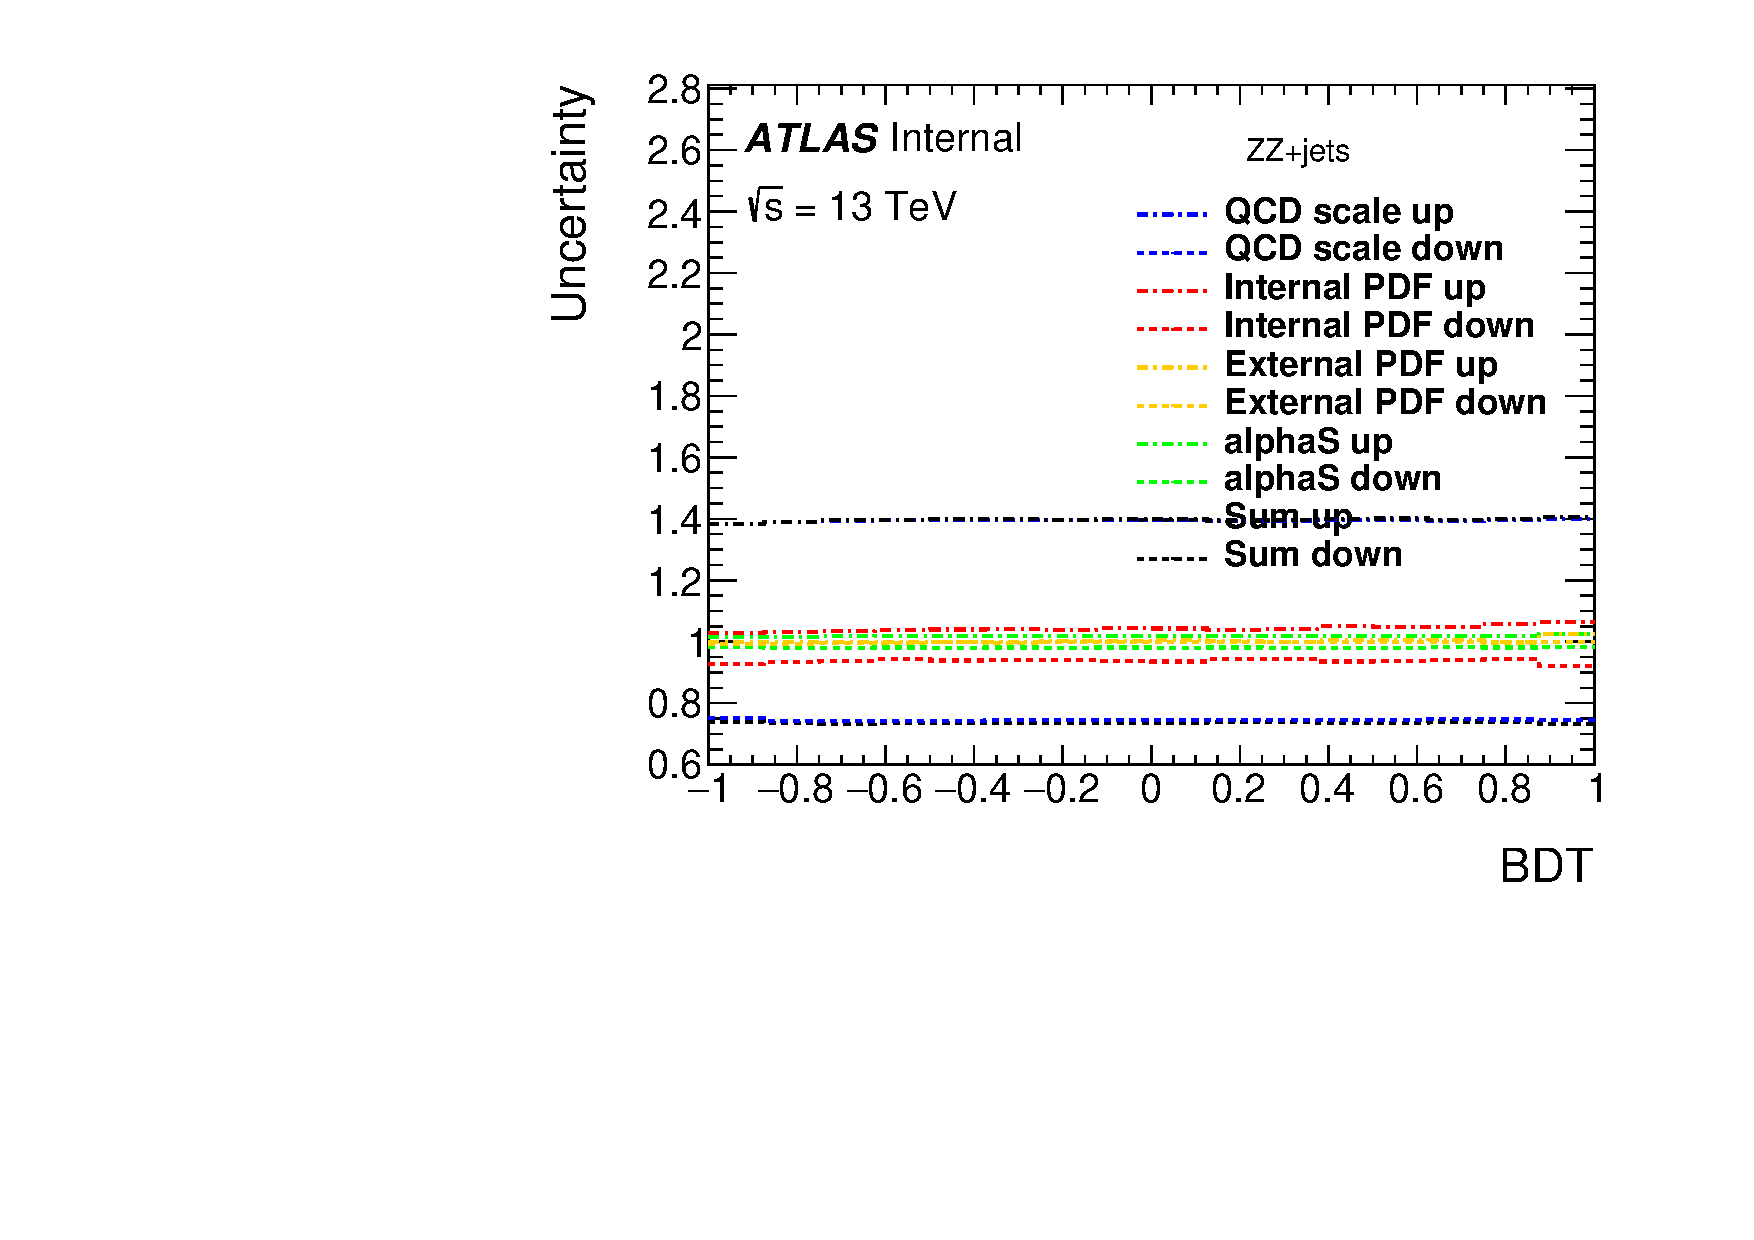
\includegraphics[width=0.42\textwidth]{figures/VBSZZ/syst/BDT_SR_linear.pdf}
  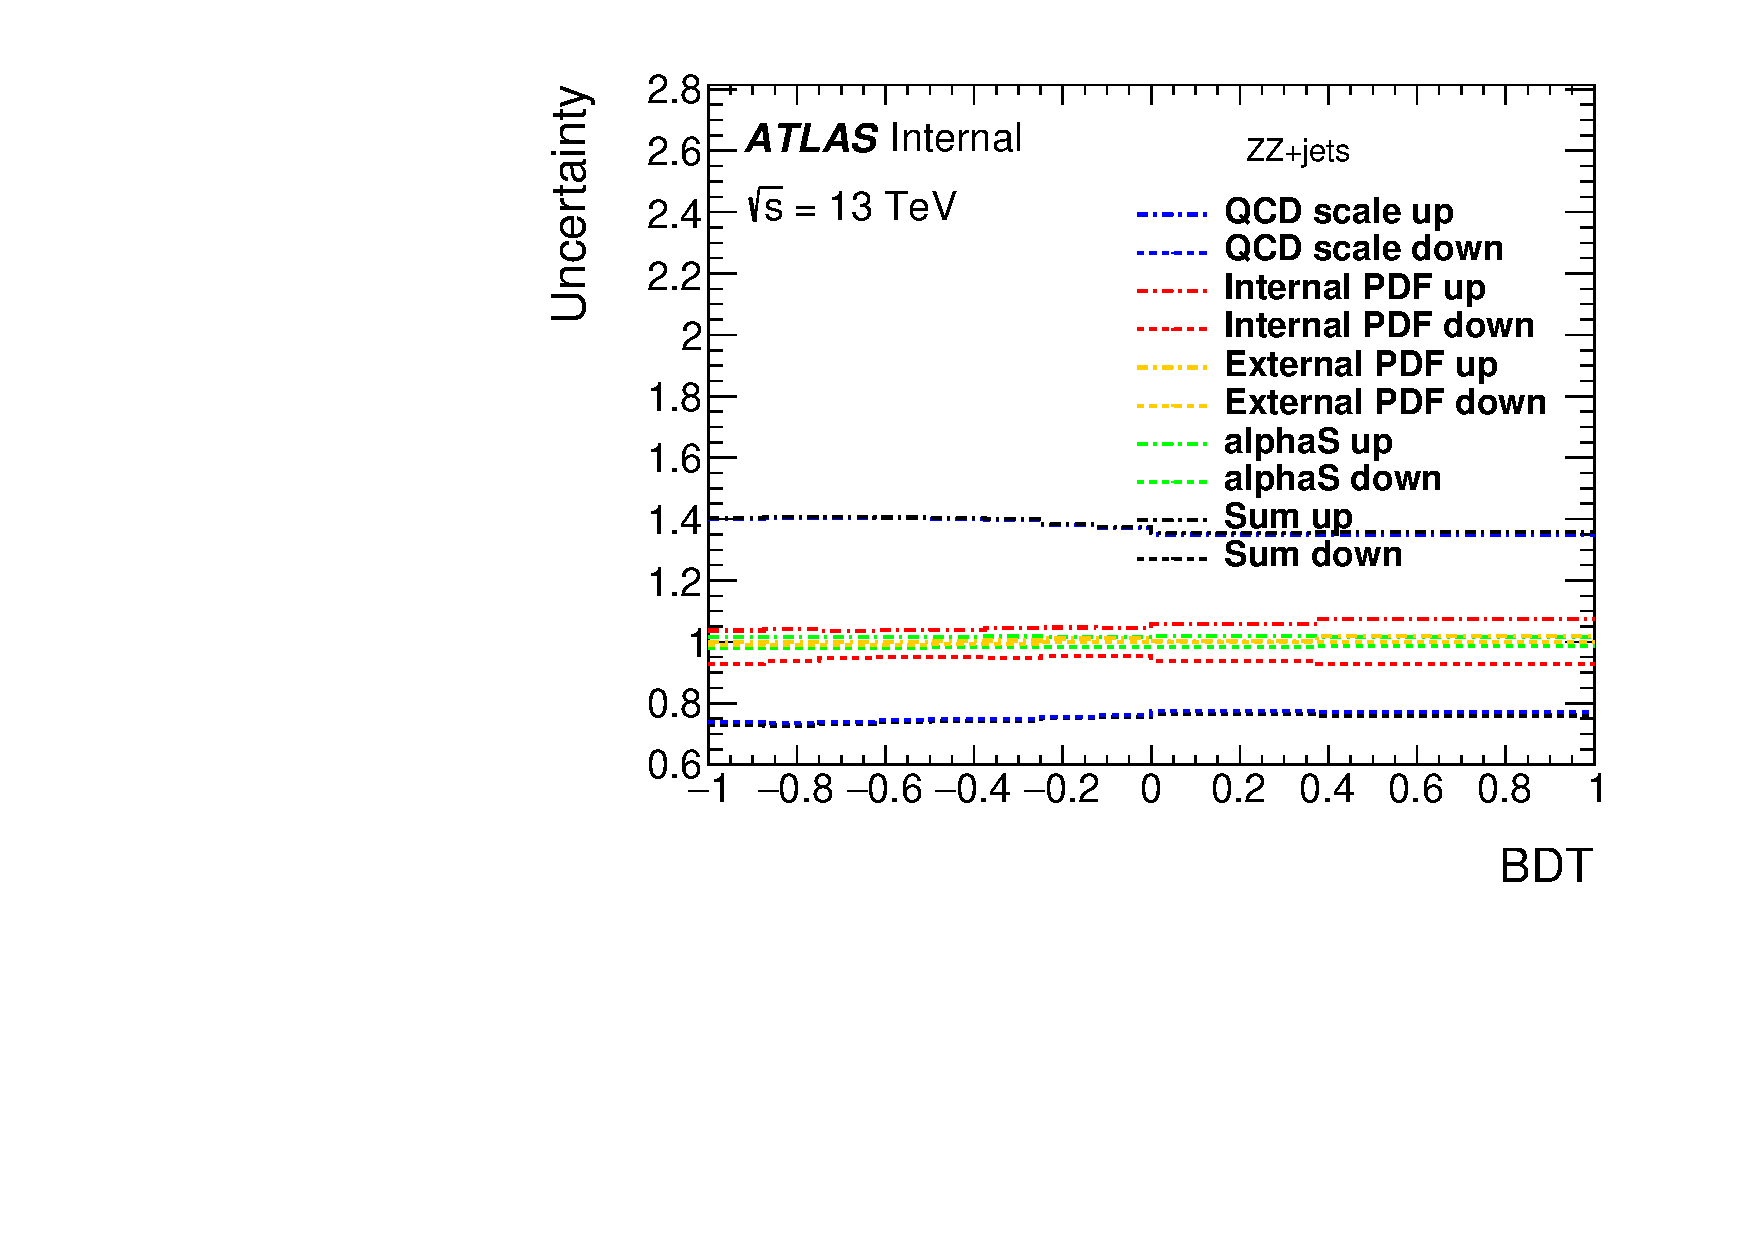
\includegraphics[width=0.42\textwidth]{figures/VBSZZ/syst/BDT_CR_linear.pdf}
  \caption{The theoretical uncertainties for \ggZZ background in particle-level SR (left) and CR (right).}
  \label{fig:syst_theo_gg}
\end{figure}

\subsection{Experimental systematics}

The major experimental uncertainties are from the luminosity uncertainty, the momentum scale and resolution of leptons and jets, as well as the lepton reconstruction and selection efficiency.
Some smaller uncertainties, such as trigger efficiency and pile-up correction, are also considered.
Overall, most large systematics are from leptons and jets. 
Table~\ref{tab:syst_exp_num} lists the major systematic components from leptons are jets for major processes in \llll channel.
The total uncertainties for sources from electron, muon and jet respectively, as well as the sum (quadratic sum) of them are also summarized in this table.
\begin{table}[H]
\begin{center}
\small
\begin{tabular}{|c|c|c|c|}
\hline
name&EW-$ZZjj$&QCD $qq$-initial&QCD $gg$\\
\hline
nominal yield&20.61&76.69&13.10\\
\hline
EG\_RESOLUTION\_ALL&$\pm^{0.00\%}_{0.03\%}$&$\pm_{0.04\%}^{0.02\%}$&$\pm^{0.01\%}_{1.41\%}$\\
\hline
EG\_SCALE\_ALL&$\pm^{0.03\%}_{0.05\%}$&-0.04\%&$\pm^{0.01\%}_{0.06\%}$\\
\hline
EL\_EFF\_ID\_TOTAL\_1NPCOR\_PLUS\_UNCOR&$\pm^{2.66\%}_{2.58\%}$&$\pm^{2.60\%}_{2.53\%}$&$\pm^{2.65\%}_{2.57\%}$\\
\hline
EL\_EFF\_Iso\_TOTAL\_1NPCOR\_PLUS\_UNCOR&$\pm$0.70\%&$\pm$0.47\%&$\pm$0.42\%\\
\hline
EL\_EFF\_Reco\_TOTAL\_1NPCOR\_PLUS\_UNCOR&$\pm$0.55\%&$\pm$0.55\%&$\pm$0.63\%\\
\hline
JET\_EtaIntercalibration\_NonClosure&-0.01\%&-0.03\%&0\%\\
\hline
JET\_GroupedNP\_1&$\pm$1.97\%&$\pm^{11.82\%}_{10.14\%}$&$\pm^{16.21\%}_{12.92\%}$\\
\hline
JET\_GroupedNP\_2&$\pm$0.23\%&$\pm$1.26\%&+5.3\%\\
\hline
JET\_GroupedNP\_3&$\pm$0.55\%&$\pm$2.94\%&$\pm^{3.14\%}_{0.12\%}$\\
\hline
JET\_JER\_SINGLE\_NP&0.11\%&+5.47\%&+6.31\%\\
\hline
JET\_JvtEfficiency&$\pm$0.04\%&$\pm$0.12\%&$\pm$0.15\%\\
\hline
MUON\_EFF\_ISO\_STAT&$\pm$0.09\%&$\pm$0.08\%&$\pm$0.07\%\\
\hline
MUON\_EFF\_ISO\_SYS&$\pm$0.54\%&$\pm$0.55\%&$\pm$0.56\%\\
\hline
MUON\_EFF\_RECO\_STAT&$\pm$0.15\%&$\pm$0.19\%&$\pm$0.15\%\\
\hline
MUON\_EFF\_RECO\_STAT\_LOWPT&$\pm$0.06\%&$\pm$0.02\%&$\pm$0.03\%\\
\hline
MUON\_EFF\_TTVA\_STAT&$\pm$0.06\%&$\pm$0.07\%&$\pm$0.06\%\\
\hline
MUON\_EFF\_TTVA\_SYS&$\pm$0.03\%&$\pm$0.4\%&$\pm$0.03\%\\
\hline
MUON\_ID&$\pm$0.03\%&$\pm$0.02\%&$<$0.001\%\\
\hline
MUON\_MS&-0.05\%&$\pm^{0.04\%}_{0.01\%}$&$<$0.001\%\\
\hline
MUON\_SAGITTA\_RESBIAS&$\pm$0.01\%&$\pm$0.02\%&$<$0.001\%\\
\hline
MUON\_SAGITTA\_RHO&+1.13\%&-0.73\%&$\pm$1.00\%\\
\hline
MUON\_SCALE&$\pm$0.02\%&$\pm^{0.03\%}_{0.02\%}$&$<$0.001\%\\
\hline
PRW\_DATASF&$\pm$0.5\%&$\pm^{0.42\%}_{1.02\%}$&$\pm^{2.17\%}_{1.46\%}$\\
\hline
\hline
Electron Exp&$\pm^{2.8\%}_{2.7\%}$&$\pm^{2.70\%}_{2.62\%}$&$\pm^{2.75\%}_{2.64\%}$\\
\hline
Muon Exp&$\pm$1.3\%&$\pm$1.3\%&$\pm$1.04\%\\
\hline
Jet Exp&$\pm$2.0\%&$\pm^{13.39\%}_{10.64\%}$&$\pm^{18.54\%}_{13.57\%}$\\
\hline
\hline
Total experimental uncertainties &$\pm^{3.7\%}_{4.0\%}$&$\pm^{13.72\%}_{11.11\%}$&$\pm^{18.90\%}_{13.57\%}$\\
\hline
\end{tabular}
\caption{
Experimental uncertainties in 4l channel (normalized to 139~\ifb).
The "Electron Exp", "Muon Exp" and "Jet Exp" represent the quadrature of the respective sources from electron, muon, and jets.
}
\label{tab:syst_exp_num}
\end{center}
\end{table}

In addition, the uncertainty of the combined 2015$~$2018 integrated luminosity is 1.7\%\cite{ATLAS-CONF-2019-021},
obtained using the LUCID-2 detector\cite{Avoni_2018} for the primary luminosity measurements.

An systematic uncertainty for MD distribution with different pile-up ($<\mu>$) is also been considered,
by comparing the distribution between events with low and high pile-up conditions.
A boundary of $<\mu> = 33$ is used to defined low/high pile-up according to the average $<\mu>$ for signal (about 34.5) and QCD background (about 33).
Figure~\ref{fig:syst_exp_pu} shows the MD distribution in SR (left) and QCD CR (right), the difference as function of MD is then taken into account as additional shape uncertainty for statistical fit.
\begin{figure}[H]
  \centering
  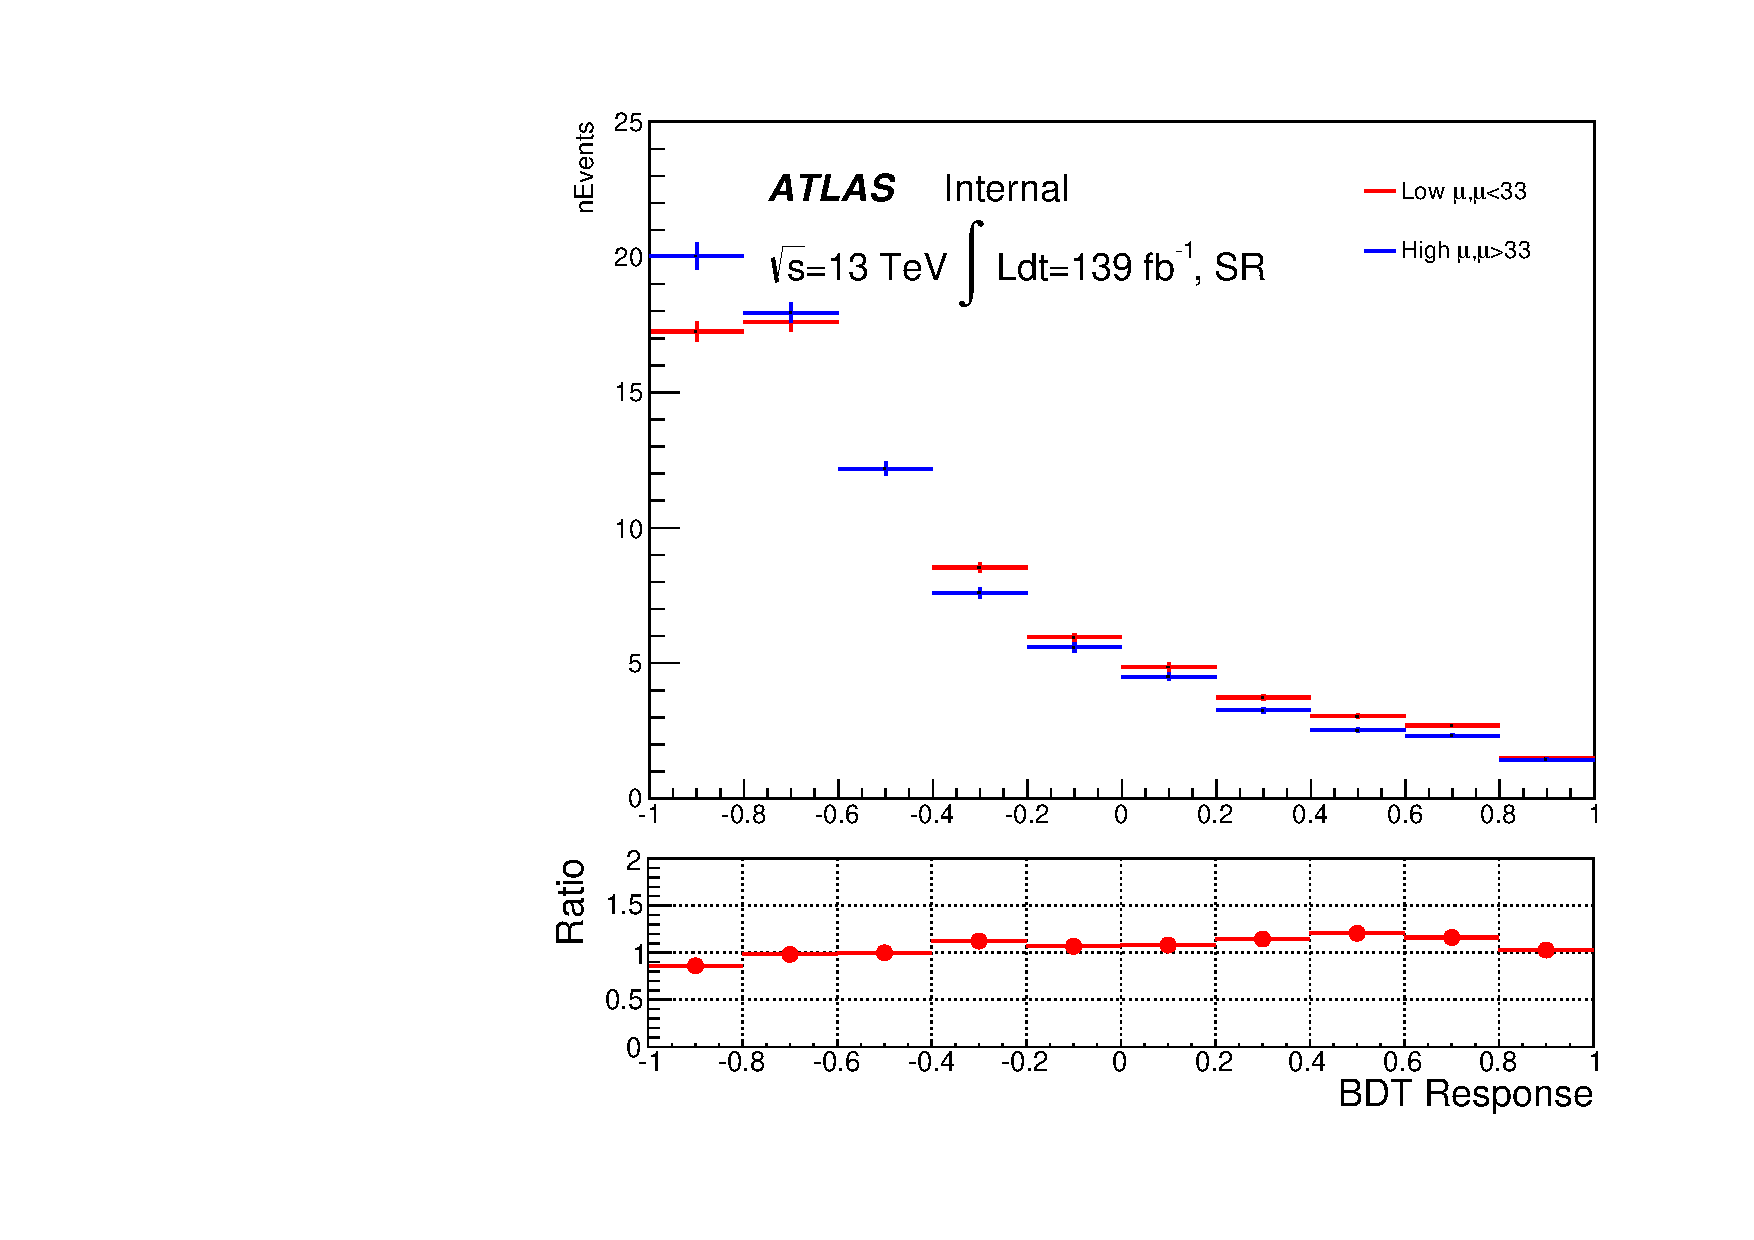
\includegraphics[width=0.42\textwidth]{figures/VBSZZ/syst/pu_uncer_BDT_SR.pdf}
  \includegraphics[width=0.42\textwidth]{figures/VBSZZ/syst/pu_uncer_BDT_CR.pdf}
  \caption{MD distribution between low and high pile-up events for SR (left) and CR (right).}
  \label{fig:syst_exp_pu}
\end{figure}

Moreover, a conservative uncertainty is signed to QCD-$ZZjj$ process by comparing the sample modelled by \textsc{Sherpa} generator (nominal) to \MGMCatNLO.
The MD shape differences for both SR (left) and QCD CR (right) are shown in figure~\ref{fig:sys_exp_shmg}.
The modelling uncertainty is calculated from the envelop of MD shape difference between nominal and alternative samples as function of MD.
\begin{figure}
  \centering
  \includegraphics[width=0.42\textwidth]{figures/VBSZZ/syst/BDT_shape_nor_linear_SR.pdf}
  \includegraphics[width=0.42\textwidth]{figures/VBSZZ/syst/BDT_shape_nor_linear_CR.pdf}
  \caption{MD shape difference for QCD \qqZZ background between different \textsc{Sherpa} theoretical uncertainties and sample from \MGMCatNLO on SR (left) and CR (right).}
  \label{fig:sys_exp_shmg}
\end{figure}


\section{Measurement of fiducial cross section}
\label{sec:xsec}

The fiducial cross section for the production of inclusive $ZZjj$, which includes both EW and QCD components, is then measured.

The defination of fiducial volume, which is used for cross section measurement, follows closely to the detector-level selection
but use physics objects in "particle-level", which are reconstructed in simulation from stable final-state particles,
prior to their interactions with the detector.
For electrons and muons, QED final-state radiation is for the most part recovered 
by adding the four-momenta of surrounding photons that are not originating from hadrons and within an angular distance $\Delta R < 0.1$
to the lepton four-momentum, called lepton "dressing".
Particle-level jets are built with anti-$k_{T}$ algorithm with radius parameter $R = 0.4$ using all final-state particles except leptons and neutrinos as inputs.
Comparing to the events selection in detector-level in section~\ref{sec:selection},
in particle-level, the selected dilepton pair mass required is relaxed to be within 60 to 120~\gev to reduce the migration effect
as well as be more compatibility with previous CMS publication\cite{2017682}.
All the other kinematics selection requirements are the same as the defination in detector-level.

\subsection{Calculation of C-factor}

C-factor is defined as the ratio between the number of selected events in detector-level and the number of particle-level events in fiducial volume (FV):
\begin{equation}
	\mathcal{C} = \frac{N_{detector-level}}{N_{FV.}}
\end{equation}
The C-factor value of each $ZZjj$ processes calculated from each individual simulation samples are listed in table~\ref{tab:xs_cf} as well as their systematics.
\begin{table}[H]
\begin{center}
   \begin{tabular}{|c|c|c|c|c|}
   \hline
   Process          & $\mathcal{C}$ & $\Delta$C(stats) & $\Delta$C(sys)        & $\Delta$C(theo)       \\
   \hline
   EWK ZZjj         & 0.663         & $\pm$0.002       & $\pm^{0.032}_{0.031}$ & NA                    \\
   \hline
   QCD \qqZZ        & 0.702         & $\pm$0.003       & $\pm^{0.061}_{0.051}$ & $\pm^{0.015}_{0.018}$ \\
   \hline
   QCD \ggZZ        & 0.741         & $\pm$0.021       & $\pm^{0.143}_{0.072}$ & $\pm{0.002}$          \\
   \hline
\end{tabular}
\end{center}
\caption{C Factor of different $ZZjj$ processes.}
\label{tab:xs_cf}
\end{table}

Then the $\mathcal{C}$ from different processes are combined together to be used as inputs for cross section calculation:
\begin{equation}
	\mathcal{C} = \Sigma_{i} \frac{N_{FV.}^{i}}{\Sigma_{j} N_{FV.}^{j}} \times \mathcal{C}_{i} = 0.699\pm0.003(stats.)\pm^{0.011}_{0.013}(theo.)\pm0.028(exp.)
\end{equation}
The stats. refers to the statistical uncertainty from MC simulation statistics.
The theo. and exp. denote the theoretical and experimental uncertainties described in section~\ref{sec:systematics}.

\subsection{Result of fiducial cross section}

The cross section in fiducial volume is computed as:
\begin{equation}\label{eq:xs}
	\sigma^{FV.} = \frac{N_{data} - N_{bkg}}{\mathcal{C} \times Lumi}
\end{equation}
where $N_{data}$ and $N_{bkg}$ denote the number of events selected from detector-level selection from data and sum of backgrounds,
and $\mathcal{C}$ is the C-factor calculated above, Lumi represents the integrated luminosity of data 2015$~$2018 of 139~\ifb.

As shown in table~\ref{tab:yield_prefit}, in inclusive measurement, only "Others" represents background, 
processes of EW-ZZjj, QCD-\qqZZ and QCD-\ggZZ are signals.
Table~\ref{tab:xs} shows the fiducial cross section for \llll channel measured from equation~\ref{eq:xs}, 
as well as the predicted cross section measured from signals MC directly.
\begin{table}[!htbp]
\begin{center}
\scalebox{0.90}{
\begin{tabular}{ c | c}
\hline
\hline\noalign{\smallskip}
Measured fiducial $\sigma$ [fb] & Predicted fiducial $\sigma$ [fb] \\
\noalign{\smallskip}\hline\noalign{\smallskip}
$1.27 \pm 0.12(\mathrm{stat}) \pm 0.02(\mathrm{theo}) \pm 0.07(\mathrm{exp}) \pm 0.01(\mathrm{bkg}) \pm 0.03(\mathrm{lumi})$ & $1.14 \pm 0.04(\mathrm{stat}) \pm 0.20(\mathrm{theo})$ \\
\noalign{\smallskip}\hline
\hline
\end{tabular}}
\end{center}
\caption{
Measured and predicted fiducial cross-sections in \lllljj final-state.
Uncertainties due to different sources are presented.
}
\label{tab:xs}
\end{table}
The measured cross section has a total uncertainty of 11\%, and is found to be compatible with SM prediction.
The data statitic is still dominanted for the measurement.

\section{Search for EW-$ZZjj$}

Figure~\ref{fig:scaled_mjj} represents the $\mjj$ distribution in SR (left) and QCD CR (right),
where the normalization of EW and QCD processes are scaled according to their observed value explained later in this section.
High $\mjj$ region is more sensitive for EW-$ZZjj$ events detection from this figure.
Figure~\ref{fig:scaled_mzz} shows the spectrum of invariant mass of \llll system ($\mzz$) in SR.
\begin{figure}[!htbp]
\begin{center}
\includegraphics[width=0.32\textwidth]{figures/VBSZZ/fit/MJJ_4l_SR.pdf}
\includegraphics[width=0.32\textwidth]{figures/VBSZZ/fit/MJJ_4l_QCD_CR.pdf}
\end{center}
\caption{Observed and expected \mjj distributions in SR (left) and QCD CR (right).
        The error bands include the expected experimental and theoretical uncertainties.
        The error bars on the data points show the statistical uncertainty on data.
        The contributions from the QCD and EW production of $ZZjj$ events are scaled by 0.96 and 1.35, respectively,
        which correspond to the observed normalization factors in the statistical fit to the combined channel.
        The last bin includes the overflow events.
        }
\label{fig:scaled_mjj}
\end{figure}

\begin{figure}[!htbp]
\begin{center}
\includegraphics[width=0.4\textwidth]{figures/VBSZZ/fit/MZZ_4l_SR.pdf}
\end{center}
\caption{Observed and expected $\mzz$ spectrum in SR.
        The error bands include the expected experimental and theoretical uncertainties.
        The error bars on the data points show the statistical uncertainty on data.
        The contributions from the QCD and EW production of $ZZjj$ events are scaled by 0.96 and 1.35, respectively,
        which correspond to the observed normalization factors in the statistical fit to the combined channel.
        The last bin includes the overflow events.
        }
\label{fig:scaled_mzz}
\end{figure}

\subsection{MD discriminant}

To further separate the EW-$ZZjj$ component from QCD-$ZZjj$, a MD based on \textit{Gradient Boosted Decision Tree (BDTG)} algorithm\cite{Coadou_BDT} 
is trained with simulated events via TMVA framework\cite{Speckmayer_2010}.
For \llll channel, training is performed between EW (signal) and QCD (background) processes.
Twelve event kinematic variables sensitive to the characteristics of the EW signal is used as input features in training. 
Table~\ref{tab:bdt_features} listed those input variables with the order of their ranking provide by TMVA tool.
The jet-related information provides larger sensitive in \llll final-state.
\begin{table}[h]
\begin{center}
\renewcommand\arraystretch{1.8}
\begin{tabular}{p{1cm}|p{2cm}|p{8cm}}
\hline
\hline
Rank & Variables                    & Description 			\\ \hline
1    & \mjj                         & Dijet invariant mass 		\\ \hline
2    & $p_{T}^{j1}$                 & \pT of the leading jet		\\ \hline
3    & $p_{T}^{j2}$                 & \pT of the sub-leading jet	\\ \hline
4    & $\frac{p_{T}(ZZjj)}{H_{T}(ZZjj)}$  & \pT of the $ZZjj$ system divided by the scalar \pT sum of Z bosons and two jets \\ \hline
5    & $y_{j1} \times y_{j2}$       & Product of jet rapidities		\\ \hline
6    & \dyjj                        & Rapodity difference between two jets \\ \hline
7    & $Y_{Z2}^{*}$                 & Rapidity of the second Z boson \\ \hline
8    & $Y_{Z1}^{*}$                 & Rapidity of the Z boson reconstructed from the lepton pair with the mass closer to the Z boson mass \\ \hline
9    & $p_{T}^{ZZ}$                 & \pT of 4l system \\ \hline
10   & $m_{ZZ}$                     & Invariant mass of 4l system \\ \hline
11   & $p_{T}^{Z1}$                 & \pT of the Z boson reconstructed from the lepton pair with the mass closer to the Z boson mass \\ \hline
12   & $p_{T}^{\ell 3}$             & \pT of the third lepton \\ \hline
\hline
\hline
\end{tabular}
\caption{Input features for the training of MD. }
\label{tab:bdt_features}
\end{center}
\end{table}
Then the MD distributions in both SR and QCD CR region are used for statistical fit.

\subsection{Profile likelihood ratio method}

To examine the compatibility between data and the signal-plus-background hypothesis, 
a test statistic is drived by using the profile likelihood ratio method.
%The likelihood function is the product of all the Poisson probability density functions built in individual MD bins given as:
The binned likelihood function is given as"
\begin{equation}
	\mathcal{L}(\mu,\sigma) = \prod_{i}^\mathrm{bins} \mathcal{L}_{\mathrm{poiss}}(N_{\mathrm{data}}\,|\,\mu s(\theta)+b(\theta))_{i} \times \mathcal{L}_{\text{gauss}}(\theta)_{i}
\end{equation}
where the Poisson term presents the statistical fluctuations of the data 
and a Gaussian term models the pdf of auxiliary measurement to constrain the systematics.
$\mu$ denotes the signal strength of EW-$ZZjj$ process, computed as the ratio between measured (expected) cross section to the SM prediction.
$\theta$ presents the nuisance parameter, which is the set of parameters that parameterize the effect of systematic uncertainties described in section~\ref{sec:systematics}.
$N_{data}$ is the number of selected data events, while the $s(\theta)$ is the expected signal yield and $b(\theta)$ is the expected background yield as the function of nuisance parameters.

The test statistic $q_{\mu}$ is defined as:
\begin{equation}
	q_\mu = -2 \ln \left( \dfrac{\mathcal{L}(\mu,\hat{\hat{\theta}}_{\mu})}{\mathcal{L}(\hat{\mu},\hat{\theta})} \right)
\end{equation}
in which $\mathcal{L}(\hat{\mu},\hat{\theta})$ is the unconditional likelihood with respect to both $\mu$ and $\theta$,
and $\mathcal{L}(\mu,\hat{\hat{\theta}}_{\mu})$ is the conditional likelihood for a constant $\mu$.
Signal-like data distributions are more likely to have a low test-statistic ($q_\mu$ close to 0) 
while the contributions of background-like data have a larger $q_\mu$.
Under the background-only hypothesis, the compatibility of the observed (Asimov) data with the prediction 
is calculated to obtain the observed (expected) significance respectively.

\subsection{Fitting procedure}

A profile likelihood fit is performed on MD discriminant to extract the EW-$ZZjj$ signal from backgrounds.
%The fit combined the observed and expected measurements from both \llll and \llvv channel from EW-ZZ production to gain more statistic.
The binning of MD distributions in SR is optimized to maximize the sensitive for detecting EW signal.
The normalization of QCD-$ZZjj$ production ($\mu_{QCD}^{llll}$) in \llll channel is varied simultaneously in the fit in SR and QCD CR as described in section~\ref{sec:background}.
The signal strength of EW-$ZZjj$ production ($\mu_{EW}$) is taken as parameter of interest and floated in the fit.
The effects of the uncertainties related to normalizations and shapes described previously in section~\ref{sec:systematics} 
of background processes in the MD distribution are all taken into account.

In most case, a common nuisance parameter is used for each source of systematic in all bins and all channels.
The statistical uncertainties for simulated samples are uncorrelated among all bins, and the background uncertaities only applied to their corresponding backgrounds.
For combination between two channels, the theoretical uncertainties between \llll and \llvv are uncorrelated due to different fiducial volumes defination.
Furthermore, to be more conservative, the generator modelling uncertainty for QCD-$ZZjj$ production mentioned in section~\ref{sec:systematics}
is separated to be two nuisance parameters in low and high MD region.

\subsection{Result of statistical fit}

The statistical fit is performed both in individual \llll channel, as well as the combination between \llll and \llvv channel to gain more statistic.
The results of statistical fit for \llll channel and the combined channel are presented in table~\ref{tab:fit_result}.
The \llvv analysis will not be talked about in this thesis, but more details can refer to \cite{ATLAS:2019vrv}.
To drive expected results, the oberved data is used for QCD CR to extract normalization factor of QCD component ($\mu_{QCD}^{llll}$),
while in SR, asimov data built from background prediction and signal model with SM assumed cross section is used.
\begin{table}[!htbp]
\begin{center}
\begin{tabular}{c|c|c|c}
\hline
                 & $\mu_{\mathrm{EW}}$ &  $\mu^{\ell\ell\ell\ell jj}_{\mathrm{QCD}}$   &  Significance Obs. (Exp.) \\
\hline
\lllljj          & $1.54 \pm 0.42$     &  $0.95 \pm 0.22$                              &  5.48 (3.90) $\sigma$     \\
\hline
Combined         & $1.35 \pm 0.34$     &  $0.96 \pm 0.22$                              &  5.52 (4.30) $\sigma$     \\
\hline
\end{tabular}
\end{center}
\caption{
Observed \muEW and \muQCD, as well as the observed and expected significance from the individual \lllljj channel, and the combined fits.
The full set of systematic uncertainties is included.
}
\label{tab:fit_result}
\end{table}
For \llll channel, the background-only hypothesis is rejected at 5.5$\sigma$ (3.9$\sigma$) for data (expectation),
which leads to the observation of EW-$ZZjj$ production.
Figure~\ref{fig:fit_MD} shows the post-fit MD distributions for \llll channel in SR (left) and QCD CR (right).
The EW-$ZZjj$ cross section measured in \llll channel is extracted to be $0.94 \pm 0.26$~fb.
\begin{figure}[!htbp]
\begin{center}
\includegraphics[width=0.42\textwidth]{figures/VBSZZ/fit/BDT_4l_SR_postFit.pdf}
\includegraphics[width=0.42\textwidth]{figures/VBSZZ/fit/BDT_4l_QCD_CR_postFit.pdf}
\end{center}
\caption{Observed and expected multivariate discriminant distributions after the statistical fit in the \llll SR (left) and QCD CR (right).
        The error bands include the experimental and theoretical uncertainties,
        as well as the uncertainties in \muEW and \muQCD.
        The error bars on the data points show the statistical uncertainty on data.
        }
\label{fig:fit_MD}
\end{figure}

Figure~\ref{fig:event_display} depicts the display of an event candidate of EW-$ZZjj$ production in $2e2\mu$ final state with two jets in forward and backward region, and with a MD value from 0.875 to 1.0.
\begin{figure}[!htbp]
\begin{center}
\includegraphics[width=1.0\textwidth]{figures/VBSZZ/fit/resize_340368_454611985_v3.pdf}
\end{center}
\caption{Display of an event candidate of EW-$ZZjj$ production in $2e2\mu$ channel in last MD bin (0.875 < MD < 1.0).
         The invariant mass of the dijet (four-lepton) system is 2228 (605)~\gev. }
\label{fig:event_display}
\end{figure}

\section{Prospect study of EW-$ZZjj$ production in HL-LHC}

The High-Luminosity Large Hadron Collider (HL-LHC) project aims to increase the luminosity by a factor of 10 beyond the LHC’s design value 
to increase the potential for discoveries after 2025.
The expected luminosity will reach 3000~\ifb~with the centre-of-mass energy of 14~\tev.

As introduced in previous sections, with full run-2 data of 139~\ifb collected by ATLAS detector at the LHC, 
the EW-$ZZjj$ production is the last channel of observation for VBS processes with massive bosons 
due to its very low cross section in $ZZ$ channel.
So we expect that this channel will benefit significantly from the increased luminosity at the HL-LHC,
and can be studied in great details for this known mechanism.

In this section, a prospective study is performed for EW-$ZZjj$ production at the HL-LHC in the \llll channel~\cite{ATL-PHYS-PUB-2018-029}.
The study uses 3000~\ifb of simulated pp collision data at a centre-of-mass energy of 14~\tev~ as expected to be recorded by the ATLAS detector at the HL-LHC.
All simulated events are produced at particle-level, 
and the detector effects of leptons and jets reconstruction and identification are estimated by corrections
assuming the mean number of interactions per bunch crossing (<$\mu$>) of 200.

\subsection{The ATLAS detector at HL-LHC}

As the expectation of HL-LHC, the new Inner Tracker (ITk)~\cite{Collaboration:2285585}
 will extend the tracking acceptance capability of ATLAS detector to pseudorapidity ($|\eta|$) up to 4.0.
By including a forward muon trigger, the upgraded Muon Spectrometer~\cite{Collaboration:2285580} is also expected to provide 
muon identification capabilities to $|\eta|$ up to 4.0.
In addition, the new high granularity timing detector (HGTD)~\cite{Collaboration:2623663} designed to mitigate the pile-up (PU) effects 
is also expected to be installed in the forward region of $2.4 < |\eta| < 4.0$.
More details of expected performance of the upgraded ATLAS detector at the HL-LHC has been reported in Ref.~\cite{ATL-PHYS-PUB-2016-026}.

\subsection{Simulation}

The analysis is performed using particle-level events.
The samples are generated at $\sqrt{s} = 14~\tev$. %and with a fast simulation based on the setting for ATLAS detector at the HL-LHC.
The signal in this analysis is EW-$ZZjj$ process, while only the dominant irreducible background of QCD-$ZZjj$ is considered.
Both signal and background are generated using \textsc{Sherpa} with the NNPDF3.0NNLO PDF set.
The signal sample is modelled with two jets at Matrix Element (ME) level.
The background is generated with up to one (three) outgoing partons at NLO (LO) in pQCD.
As a quick study, other minor backgrounds such as fake backgrounds from \Zjet and top-quark processes, as well as Diboson without 4l final-state and Triboson processes are not considered in this analysis.
Furthermore, for hard scattering events, the pile-up collisions are set with a mean value of 200 interactions per bunch crossing.
Signal and background yields are then scaled to an integrated luminosity of 3000~\ifb~as expected at the HL-LHC.

\subsection{Event selection}

The analysis selection follows closely to the one in ATLAS run-2 analysis as described in section~\ref{sec:vbszz_selection}.
Here are some changes according to the expectation of the HL-LHC scenario for ATLAS detector:
\begin{itemize}
	\item Extend the lepton (both electron and muon) identification to $|\eta| <$ 4.0
	\item Pile-up (PU) jet suppression is applied with a PU rejection factor of 50 for all PU jets in the region of $|\eta| <$ 3.8, based on the expected ATLAS detector performance at the HL-LHC.
	\item The jets are required to have $\pT >$ 30 (70)~\gev~in the $|\eta| <$ 3.8 ($3.8 < |\eta| < 4.5)$ region.
	\item For two selected jets, tighten the $\mjj$ requirement to be $\mjj > 600$~\gev, and require $\Delta \eta_{jj} >$ 2.
\end{itemize}
In addition, a fiducial volume, used to study the expected precision of the cross-section measurements,
 is defined at particle-level with the same kinematic requirements listed above.

Table~\ref{tab:event_yield} summarized the number of selected signal and background events normalized to 3000~\ifb.
In addition to the \textit{baseline} selection listed above, to compare the different detector scenarios at the HL-LHC, two alternative selections are also studied:
\begin{enumerate}
	\item Reduce the lepton $\eta$ region to 2.7, to understand the effect due to forward lepton reconstruction and identification with the upgraded ATLAS detector.
	\item Only apply the PU jet suppression with region $|\eta| < 2.4$, to measure the improvement of \textit{baseline} by extending the rejection range of PU jets at the HL-LHC with the installation of HGTD.
\end{enumerate}
\begin{table}[htbp]
  \small
  \centering
  \begin{tabular}{|c|c|c|c|}
    \hline
    Selection & $N_{\mathrm{EW-ZZjj}}$ & $N_{\mathrm{QCD-ZZjj}}$ & $N_{\mathrm{EW-ZZjj}}$ / $\sqrt{N_{\mathrm{QCD-ZZjj}}}$ \\
    \hline
    Baseline                                 & 432 $\pm$ 21 & 1402 $\pm$ 37   & 11.54 $\pm$ 0.58 \\
    \hline
    Leptons with $|\eta|<$ 2.7               & 373 $\pm$ 19 & 1058 $\pm$ 33   & 11.46 $\pm$ 0.62 \\
    \hline
    PU jet suppression only in $|\eta|<$ 2.4 & 536 $\pm$ 23 & 15470 $\pm$ 120 &  4.31 $\pm$ 0.19  \\
    \hline
  \end{tabular}
  \caption{
    Comparison of event yields for signal ($N_{\mathrm{EW-ZZjj}}$) and background ($N_{\mathrm{QCD-ZZjj}}$) processes, 
    and expected significance of EW-$ZZjj$ processes,
    normalized to 3000~\ifb{} data at 14~\TeV{},
    with baseline and alternative selections.
    Uncertainties in the table refer to expected data statistical uncertainty at 14~\TeV{} with 3000~\ifb{}.
  }
  \label{tab:event_yield}
\end{table}
From this table, one can see the extended track coverage increases the \lllljj events by 15 to 30\%, via improving the lepton efficiency.
But the significance of searching for EW-$ZZjj$ process does not improve so much due to the large increment of background events.

Figure~\ref{fig:kine} shows the kinematic distributions of di-jet invariant mass (\mjj), the $ZZ$ invariant mass (\mzz) and 
the $\phi$ separation of two Z bosons ($|\Delta\phi(ZZ)|$) as well as the centrality of the ZZ system.
The ZZ centrality is defined as:
\begin{equation}
  ZZ~\text{centrality} = \frac{|y_{ZZ} - (y_{j1} + y_{j2})/2|}{|y_{j1} - y_{j2}|}
\end{equation}
To measure the event yield, the top panel shows the stack distribution for EW- and QCD-$ZZjj$ processes,
while bottom panel is the ratio between two processes.
\begin{figure}[!htbp]
\centering
\subfloat[]{
\includegraphics[width=0.42\textwidth]{figures/VBSZZ/hllhc/TagJJM_final_noshape_0_ratio.pdf}
}
\subfloat[]{
\includegraphics[width=0.42\textwidth]{figures/VBSZZ/hllhc/MVV_noshape_0_ratio.pdf}
}
\\
\subfloat[]{
\includegraphics[width=0.42\textwidth]{figures/VBSZZ/hllhc/dPhiZZ_noshape_0_ratio.pdf}
}
\subfloat[]{
\includegraphics[width=0.42\textwidth]{figures/VBSZZ/hllhc/ZZCen_noshape_0_ratio.pdf}
}
\caption{
Detector-level distributions of EW- and QCD-$ZZjj$ processes with selected events in defined phase space at 14~\tev~of 
(a) \mjj,
(b) \mzz,
(c) $|\Delta\phi(ZZ)|$,
(d) ZZ centrality,
normalized to 3000~\ifb{}.
}
\label{fig:kine}
\end{figure}


\subsection{Systematics}

According to studies in section~\ref{sec:systematics}, the dominant systematic in \llll channel is from theoretical systematic for QCD-$ZZjj$ background process.
Different sizes of systematics have been studied, at a factor of 5, 10 and 30\% on background modelling.
The 5\% uncertainty is an optimal estimation when there is enough data events from QCD-enriched control region at the HL-LHC that can be used to constrain the theoretical normalization on QCD-$ZZjj$ process.
The 30\% one is a conservative estimation, in which the uncertainties are directly calculated from different PDF sets and QCD renormalization and factorization scales, following recommendation from the PDF4LHC mentioned in section~\ref{sec:systematics}.

For experimental sources, the jet systematics have been checked following the setting provided by the HL-LHC in Ref.\cite{ATL-PHYS-PUB-2016-026},
and the uncertainties are within 5\% level, which is smaller than run-2 measurement at 10\%.
Figure~\ref{fig:jet_uncer} depicts the up and down variations for jet uncertainty provided by the HL-LHC performance tool as function of dijet invariant mass ($\mjj$).
\begin{figure}
  \centering
  \includegraphics[width=0.42\textwidth]{figures/VBSZZ/hllhc/Uncer_baseline_TagJJM_ewk_linear.pdf}
  \includegraphics[width=0.42\textwidth]{figures/VBSZZ/hllhc/Uncer_baseline_TagJJM_qcd_linear.pdf}
  \caption{Jet variations on $\mjj$ distribution for EW-$ZZjj$ (left) and QCD-$ZZjj$ (right) processes
           with luminosity of 3000~\ifb at 14~\tev.
	   \textit{Upgrade Performance Function} is used to extract the uncertainties with \textit{baseline} setting.}
  \label{fig:jet_uncer}
\end{figure}
Therefore, a conservative 5\% uncertainty is used as experimental uncertainty.

Since the final result relies greatly on the uncertainties, especially the theoretical uncertainties on QCD-$ZZjj$ production.
So results with different uncertainty conditions are shown as below:
\begin{itemize}
	\item The case with statistical uncertainty of simulated samples only.
	\item The case with statistical and experimental uncertainties (5\%)
	\item The case with statistical, experimental and additional theoretical uncertainties at 5\%, 10\% and 30\% levels respectively.
\end{itemize}
Three different sources of uncertainties are treated as uncorrelated and summed up quadratically.

\subsection{Results}

In this analysis, instead of a statistical fit, the expected significance of EW-$ZZjj$ production is calculated as:
\begin{equation}
  \text{Significance} = \frac{S}{\sqrt{\sigma(B)_{stat.}^2 + \sigma(B)_{syst.}^2}},
\end{equation}
where $S$ presents the number of selected signal events,
and $\sigma(B)_{stat.}$ and $\sigma(B)_{syst.}$ denote the statistical and systematic (exp. + theo.) uncertainties from background processes.
The statistical uncertainty is computed from expected data yield with an integrated luminosity of 3000~\ifb.

Based on baseline selection of $\mjj > 600~\gev$, an additional scan over different \mjj cuts is also performed with a step of 50~\gev~
under different systematic conditions, as shown in figure~\ref{fig:mjj_scan}.
\begin{figure}[!htbp]
\centering
\includegraphics[width=0.48\textwidth]{figures/VBSZZ/hllhc/significance_noshape_0_noratio.pdf}
\caption{
The expected significance of EW-$ZZjj$ processes as a function of different \mjj cut with 3000~\ifb,
under conditions of different sizes of theoretical uncertainties on the QCD-$ZZjj$ background modelling.
The statistical uncertainty is estimated from expected data yield at 14~\tev~ with 3000~\ifb.
Different uncertainties are summed up quadratically.
}
\label{fig:mjj_scan}
\end{figure}

In addition, the expected differential cross section of EW-$ZZjj$ process is measured in the defined phase space at 14~\tev,
as a function of \mzz and \mjj, shown in figure~\ref{fig:xs_mjj_mzz}.
\begin{figure}[!htbp]
\centering
\includegraphics[width=0.48\textwidth]{figures/VBSZZ/hllhc/TagJJM_final_all_linear.pdf}
\includegraphics[width=0.48\textwidth]{figures/VBSZZ/hllhc/MZZ_all_linear.pdf}
\caption{
The projected differential cross-sections at 14~\tev~ for the EW-$ZZjj$ processes as a function of \mjj (left) and \mzz (right).
The top panel shows measurement with statistical only case,
where statistical uncertainty is estimated from expected data yield at 14~\tev~ with 3000~\ifb.
The bottom panel shows impact of different sizes of systematic uncertainties.
}
\label{fig:xs_mjj_mzz}
\end{figure}
The expected differential cross sections are calculated as:
\begin{equation}
\begin{split}
    \sigma = \frac{N_{pseudo-data} - N_{QCD-ZZjj}^{det.}}{L*C_{EW-ZZjj}}\\
  C_{EW-ZZjj} = \frac{N_{EW-ZZjj}^{det.}}{N_{EW-ZZjj}^{part.}}
\end{split}
\end{equation}
where $N_{pseudo-data}$ denotes the expected number of data events with 3000~\ifb~ luminosity at 14~\tev,
and $N_{QCD-ZZjj}$ and $N_{EW-ZZjj}$ are the number of predicted events of QCD-$ZZjj$ and EW-$ZZjj$ processes, in particle-level (part.) or detector-level (det.).
The $C_{EW-ZZjj}$ factor represents the detector efficiency for EW-$ZZjj$ processes introduced in section~\ref{sec:cf}.
The interference between EW- and QCD- $ZZjj$ processes is ignored due to its minor contribution.

The value of expected integrated cross section as well as its uncertainty under different systematic conditions are shown in table~\ref{tab:xsec}
with 3000~\ifb luminosity at 14~\tev.
The statistical uncertainty is at 10\% level when with such large luminosity.
The result is dominated by systematics and can reach 100\% level when theoretical modelling uncertainty is 30\% for QCD-$ZZjj$ processes.
\begin{table}[htbp]
  \footnotesize
  \centering
  \begin{tabular}{c|c|c|c|c|c|c}
    \hline
     & Cross section [fb] & Stat. only & Plus exp. & Plus $5\%$ theo. & Plus $10\%$ theo. & Plus $30\%$ theo. \\
    \hline
    EW-$ZZjj$ & 0.21 & $\pm0.02$ & $\pm0.04$ & $\pm0.05$ & $\pm 0.08$ & $\pm 0.21$ \\
    \hline
  \end{tabular}
  \caption{
  Summary of expected cross-section measured with different theoretical uncertainties.
  The statistical uncertainty is computed from expected data yield with 3000~\ifb~ at 14~\tev.
  Different uncertainties are treated as uncorrelated and summed quadratically.
  }
  \label{tab:xsec}
\end{table}



\clearpage
\section{Conclusion}

The fiducial cross section for inclusive $ZZjj$ production is measured in this section, with a total relative uncertainty of 11\% for the \llll final state,
and found to be compatible with the SM prediction.
The observation of electroweak production of two jets in association with a $Z$-boson pair decay to \llll final state 
using 139~\ifb of 13~\tev~pp collision data collected by ATLAS experiment at the LHC is presented in this section.
The search for electroweak production of two jets in association with a $Z$-boson pair is based on multivariate discriminants (MD) to enhance the separation between the signal and backgrounds.
In \llll final state, the background-only hypothesis is rejected with an observed (expected) significance of 5.5 (3.9)~$\sigma$,
which gives the first observation of electroweak production in $ZZjj$ channel.

In addition, the prospect study for the EW-$ZZjj$ production at the HL-LHC in the \llll channel, using 3000~\ifb~ simulated pp collision data at a centre-of-mass energy of 14~\tev~has been presented.
The precision of the expected measurements of the integrated and differential cross sections as a function of dijet or \llll invariant mass are shown.
Under the assumption of theoretical uncertainty for the QCD-$ZZjj$ processes 
and experimental uncertainty for jets being constraint at 5\% level respectively, 
with statistical uncertainty in 3000~\ifb being considered, 
the observation of the EW-$ZZjj$ process can reach a significance of 7~$\sigma$.


\chapter{Search for heavy $ZZ$ resonances in the \llll final state using pp collisions data collected by ATLAS detector from 2015$~$2018}

\section{Introduction}

A new particle was discovered by the ATLAS and CMS Collaborations at the LHC~\cite{20121, 201230} in 2012.
Both two experiments have confirmed that the properties including spin, couplings and parity of this new particle are consistent with 
Higgs boson predicted in the Standard Model (SM), which is an important milestone in understanding of the mechanism of EWSB.
Nevertheless, the possibility that this newly discoved particle is just a part of the extended Higgs sector
as predicted by various extensions in the SM cannot be ruled out.
There are many models predicted the existence of new heavy resonances decaying into dibosons, 
such as the electroweak-singlet model of a heavy spin-0 neutral Higgs boson~\cite{PhysRevD.36.3463}
and the two-Higgs-doublet models (2HDM)~\cite{BRANCO20121}, 
as well as the spin-2 Kaluza–Klein (KK) excitations of the graviton (GKK)~\cite{DAVOUDIASL200043}.

%\section{Data and MC samples}

\subsection{Data samples}

The data used in this analysis are collected by ATLAS detector at the centre-of-mass energy of 13~\tev~ during the years of 2015 to 2018.
Only events passing the latest Good Run List (GRL) released by the Data Quality group from ATLAS experiment %as listed in section~\ref{sec:vbszz_data} 
corresponding to an integrated luminosity of $139.0~\pm~2.4$~\ifb~ are used.
Table~\ref{tab:data_info} listed the recorded integrated luminosity, average and peak pile-up of each year's data.
\begin{table}[htbp]
  \centering
  \caption{Summary of the recorded integrated luminosity (lumi), average and peak pile-up (PU) of data from 2015 to 2018.}
  \label{tab:data_info}
  \begin{spacing}{0.65}
  \begin{tabular}{ccccc}
    \toprule
    Year & recorded integrated lumi  & lumi after GRL & average PU & peak PU  \\
    \midrule
    2015 & 3.86~\ifb & \multirow{2}{*}{36.2~\ifb} & 13.4 & 28.1 \\
    2016 & 35.6~\ifb & & 25.1 & 52.2 \\
    2017 & 46.9~\ifb & 44.3~\ifb & 37.8 & 79.8 \\
    2018 & 60.6~\ifb & 58.5~\ifb & 36.1 & 88.6 \\
    \bottomrule
  \end{tabular}
  \end{spacing}
\end{table}

\subsection{Background MC simulations}

Background processes considered in this analysis include $ZZ$ (\qqZZ, \ggZZ), triboson ($WWZ$, $WZZ$, $ZZZ$), \Zjet and top-quark (\ttbar, ttV) processes.

The QCD \qqZZ process is modelled using \textsc{Sherpa} 2.2.2~\cite{Gleisberg:2008ta} with the NNPDF3.0NNLO~\cite{ball2015parton} PDF,
where events with up to one (three) outgoing partons are generated at NLO (LO) in pQCD.
The production of $ZZ$ from the gluon-gluon initial state with a four-fermion loop or with an exchange of the Higgs boson, which has an order of $\alpha_{S}^{4}$ in QCD, is not included in this \textsc{Sherpa} simulation.
So a separate $gg$ induced $ZZ$ sample including the continuum background, the SM Higgs boson, and the interference contribution 
is modelled using \textsc{Sherpa} 2.2.2 with the NNPDF3.0NNLO PDF set,
and with an additional k-factor~\cite{PhysRevD.92.094028} of 1.7 applied.
The EW-$ZZjj$ production is simulated using \textsc{Sherpa} 2.2.2 with the NNPDF3.0NNLO PDF, and the $ZZZ \rightarrow \llll qq$ process is also taken into account in this sample.

The \Zjet events are generated using \textsc{Sherpa} 2.2.2 with the NNPDF3.0NNLO PDF,
in which the ME is calculated for up to two partons with NLO accuracy in pQCD and up to four partons with LO accuracy.
The \Zjet events are normalized using the next-to-next-to-leading-order (NNLO) cross section.
The triboson processes with full leptonic decays and at least four prompt charged leptons are generated using \textsc{Sherpa} 2.1.1.
For top-quark pair (\ttbar) production and the single top-quark productions in $t$-channel, $s$-channel and $Wt$-channel, \textsc{Powheg-Box}~v2 is used with the CT10 PDF.
The productions of \ttbar~in association with $Z$ boson(s) ($ttZ$) is modelled with \MGMCatNLO.

\subsection{Signal MC simulations}
\label{sec:hmhzz_signal_mc}

One model considered in this analysis is heavy spin-0 resonance under the Narrow Width Approximation (NWA) simulated using \textsc{Powheg-Box}~v2 MC event generator with the CT10 PDF.
The gluon-gluon fusion (ggF) production mode and vector-boson fusion (VBF) production mode are calculated separately with matrix elements up to NLO in QCD.
The \textsc{Powheg-Box} is interfaced to \textsc{Pythia8} for parton showering, and for decaying the Higgs boson into the $H \rightarrow ZZ \rightarrow \llll$ final states.
Events of NWA signal are generated at mass points between 200~\gev~to 2000~\gev~using the step of 100 (200)~\gev~up to (above) 1~\tev~in both ggF and VBF production modes.

In addition, heavy Higgs boson events under the Large Width Approximation (LWA) with widths of 1\%, 5\%, 10\% and 15\% of the boson mass are generated using \MGMCatNLO~2.3.2 interfaced to \textsc{Pythia8}.
Only ggF production is considered.
Mass points between 400~\gev~to 2000~\gev~are simulated with the step of 100 (200)~\gev~ up to (above) 1~\tev.
To describe jet multiplicity, \MGMCatNLO~is used to simulated process of $pp\to H + \geq2\text{jets}$ at NLO in QCD with the FxFx merging scheme~\cite{Frederix2012}.

Spin-2 Kaluza–Klein (KK) gravitons (\Graviton) from the Bulk Randall–Sundrum model~\cite{graviton} are also studied in this analysis.
Events are generated by \MGMCatNLO at LO in QCD, which is then interfaced to \textsc{Pythia8} for parton showering.
The \Graviton-gluon coupling \kOverMpl, where $k$ is the curvature scale of the extra dimension and \Mpl~is the reduced Planck mass, is set to 1.
The width of the resonance is correlated with the coupling \kOverMpl~and in this configuration is around ∼ 6\% of its mass. 
The mass of the \Graviton~is the only free parameter in this simplified model.
Mass points between 600~\gev~ to 2~\tev~ with 200~\gev~ spacing were generated.

%\section{Analysis selections}
\label{sec:hmhzz_selection}

\subsection{Objects selection}
\label{sec:hmhzz_objsel}

Similar to VBSZZ analysis in section~\ref{sec:vbszz_selection}, the selection of this analysis relies on the definition of multiple objects: \textit{electrons}, \textit{Muons}, and \textit{jets}.
Details of definitions for each object are described as below:

\textbf{Electron:}
As described in section~\ref{sec:electron}, electrons are reconstructed from energy deposits in the EM calorimeter matched to a track in the inner detector.
The electron candidates satisfying the \textit{Loose} criterion valuing by the likelihood-based (LH) method are selected,
with a selection efficiency ranging from 90\% for transverse momentum $\pt = 20~\gev$ to 96\% for $\pt > 60~\gev$.
In addition, the electrons are required to have $p_{T} > 7~\gev$, $|\eta| < 2.47$ and $|z_{0} sin\theta|$ < 0.5 mm.

\textbf{Muon:}
To increase the acceptance range in reco-level for \llll channel, all four types of muons
(CB, ST, CT, ME muons, described in section~\ref{sec:muon}) are used.
The CT muons are required to pass $p_{T} > 15~\gev$ and $|\eta| < 0.1$, while the ST muons are also limited in $|\eta| < 0.1$ region.
The ME muons are only used in the region of $2.5 < |\eta| < 2.7$.
And at most one CT, ST or ME muon is allowed in one \llll quadruplet.
The Muon candidates are required to pass $p_{T} > 5~\gev$ and $|\eta| < 2.7$,
and satisfy the \textit{Loose} identification criterion with an efficiency of at least 98.5\%.
The impact parameter requirements of $|d_{0}|$ < 1 mm and $|z_{0} sin\theta|$ < 0.5 mm are further applied.

\textbf{Jets:}
Jets are clustered using the anti-$k_t$ algorithm with radius parameter $R$ = 0.4 implemented in the \textsc{FastJet} package as described in section~\ref{sec:jet}. 
The `particle flow' (PFlow) objects~\cite{PERF-2015-09}, which combines measurements from both the tracker and the calorimeter, are used as inputs to the \textsc{FastJet} package.
The energy deposited in the calorimeter by all charged particles is removed, and the jet reconstruction is performed on an ensemble of PFlow objects
consisting of the remaining calorimeter energy and tracks which are matched to the hard interaction.
This improves the accuracy of the charged-hadron measurement, while retaining the calorimeter measurements of neutral-particle energies. 
Compared to only using topological clusters, jets reconstructed with the particle flow algorithm with $\pt > 30~\gev$ have approximately 10\% better transverse momentum resolution.
The jets used in this analysis are then required to have $\pt > 30~\GeV$ and $|\eta | < 4.5$.
To further reduce the effects of pile-up jets, a jet vertex tagger (JVT) is applied to jets with $p_{T} <$ 60~\gev~and $|\eta| < 2.4$.

\textbf{Overlap removal:}
As the selected jet and lepton candidates can be reconstructed from same detector information, an overlap-removal procedure is applied.
For electron and muon sharing the same ID track, the electron is selected in the case that the muon is calorimeter-tagged and does not have a MS track, or is a segment-tagged muon, otherwise the muon is selected.
The jet overlapping with electron (muon) within a cone of size of $\Delta R\equiv \sqrt{(\Delta \eta)^2 + (\Delta \phi)^2}= 0.2 (0.1)$ are removed.

%% ========================================================================
\subsection{Event selection}
\label{sec:hmhzz_eventsel}

First of all, the four-lepton events are required to pass single or multi-lepton triggers.
Due to the increasing of peak luminosity and pile-up, the \pt and \et thresholds of triggers increase slightly during the data-taking periods from 2015 to 2018.
Table~\ref{tab:hmhzz_triggers} summarizes the triggers used for \llll channel. 
The overall trigger efficiency for selected signal events passing final selection is around 98\%.

\begin{table}[!htbp]
\begin{center}
\caption{Summary of the $\pt$ ($E_T$) trigger thresholds (in~\gev) employed for the muon (electron) trigger selection in the year of 2015, 2016, 2017, and 2018.}
\label{tab:hmhzz_triggers}
\adjustbox{max width=\textwidth}{%
\vspace{0.2cm}
\begin{tabular}{|l|c|c|c|c|}
\hline
Trigger item& \multicolumn{4}{c|}{Trigger threshold}\\
& \multicolumn{1}{c|}{2015}& \multicolumn{1}{c|}{2016}& \multicolumn{1}{c|}{2017}& \multicolumn{1}{c|}{2018}\\
\hline
single muon&        $\mu 20$;~~$\mu 50$;~~$\mu 60$&
                    $\mu 24$;~~$\mu 26$;~~$\mu 40$;~~$\mu 50$&
                    $\mu 26$;~~$\mu 50$;~~$\mu 60$&
                    $\mu 26$;~~$\mu 50$;~~$\mu 60$\\
single electron&    $e24$;~~$e60$;~~$e120$&
                    $e26$;~~$e60$;~~$e140$;~~$e300$&
                    $e26$;~~$e60$;~~$e140$;~~$e300$&
                    $e26$;~~$e60$;~~$e140$;~~$e300$\\
\hline
dimuon&             $2\mu 10$;~~$\mu 18 \_\mu8$&
                    $2\mu 10$;~~$2\mu 14$;~~$\mu 22 \_\mu8$&
                    $2\mu 14$;~~$\mu 22 \_\mu8$&
                    $2\mu 14$;~~$\mu 22 \_\mu8$\\
dielectron&         $2e12$&
                    $2e15$;~~$2e17$&
                    $2e17$;~~$2e24$&
                    $2e17$;~~$2e24$\\
\hline
electron-muon&
                    $e24 \_\mu 8$&
                    $e24 \_\mu 8$;~~$e26 \_\mu 8$&
                    $e26 \_\mu 8$&
                    $e26 \_\mu 8$\\
                    $ $&
                    \multicolumn{4}{c|}{$e17\_\mu 14$;~~$e7 \_\mu24$;~~$2e12 \_\mu 10$;~~$e12 \_2\mu10$}\\
\hline

trimuon&
                    $\mu18\_2\mu4$&
                    $\mu11\_2\mu4$;~~$\mu6\_2\mu4$;~~$\mu 20\_2\mu 4$;~~$3\mu4$&
                    $4\mu4$;~~$\mu 20\_2\mu 4$;~~$3\mu4$&
                    $\mu 20\_2\mu 4$\\
                    $ $&
                    \multicolumn{4}{c|}{$3\mu6$}\\
\hline

trielectron&        $e17\_2e9$&
                    $e17\_2e9$;~~$e17\_2e10$&
                    $e24\_2e12$&
                    $e24\_2e12$\\

\hline

\end{tabular}}
\end{center}
\end{table}

The \llll quadruplets are formed by two opposite-sign, same-flavour (OSSF) lepton pairs ($\ell^{+}\ell^{-}$).
The $\pT$ threshold of first three leading leptons are required to be 20, 15 and 10~\gev.
If there are more than one combination of lepton pairing in quadruplet, the pairing is selected by keeping it with the mass of lepton pairs closest (leading pair, refers as $m_{12}$) and second closest (sub-leading pair, refers as $m_{34}$) to Z boson mass.
The mass of leading pair is required to satisfy $50 < m_{12} < 106~\gev$, while the sub-leading pair is required to be less than 115~\gev~ and larger than 50~\gev. 

The two lepton pairs in quadruplet are required to have angular separation with $\Delta R > 0.1$.
To suppress the contribution from $J/\psi \rightarrow \ell\ell$ decays, for $4\mu$ and $4e$ quadruplets, the events are rejected if any opposite-sign same-flavour lepton pair is found with mass below 5~\gev.
If there are more than one quadruplets from different channels in event at this point, the one with highest expected signal rate is selected in the order of $4\mu$, $2e2\mu$, $4e$.
The transverse impact-parameter significance ($|d_0|/\sigma_{d_0}$) for muons (electrons) is than required to be smaller than 3 (5) to suppress the backgrounds from heavy-flavour hadrons.

In addition, the track- and calorimeter- based isolation criteria is required for all electrons and muons to further suppress the reducible backgrounds of \Zjet and \ttbar.
For lepton isolation selection, the two track- and calorimeter- based variables, $E_{T}^{topocone}$ and $p_{T}^{varcone}$ as described in section~\ref{sec:muon} (section~\ref{sec:electron}) for muons (electrons), are vulnerable to pileup.
For track-based variable, this is because of additional tracks in the event.
The definition of $p_{T}^{varcone}$ attempts to limit the tracks used in the calculation to those from the vertex via a loose cut of $|z_0\sin(\theta)| < 3$,
which proved to be too loose in new pile-up regime 2017 and 2018 datasets.
So new track-based variable is used, 
by adding a requirement that the track be used in determining the vertex, or that, if not, it both pass the cut on $|z_0\sin(\theta)|$ and not be used in determining any other vertex,
which makes the track-based variable to be more isolation-robust in the high pile-up regime.
The new variable is named as ptvarcone[cone]$\_$TightTTVA$\_$pt[\pt cut], where [cone] is the cone size and [\pt cut] is the cutoff for including tracks in the calculation.

For calorimeter-based variable, the calculation of $E_{T}^{topocone}$ corrects the pile-up effects by subtracting an average pileup contribution computed over the whole detector.
But with the increasing of energy density of pile-up events, the root mean square (RMS) of $E_{T}^{topocone}$ variable increases,
which leads to the increment of possibility that the pile-up fluctuations are not be accounted for correctly.
One possible solution is that use particle-flow (PFlow) method to calculate the calorimeter isolation.
As part of PFlow reconstruction process, it assigns the clusters to tracks which improves the track-cluster association for better determination of the raw value of the \et in the cone.
And using PFlow jets to calculate the pileup correction provides a further improvement.
So a resulting variable named neflowisol[cone] is used.
Finally, a requirement of isolation, called \textit{FixedCutPFlowLoose}, which gives better performance in high piup-up condition is applied to electrons and muons as: \\
	( max ( ptcone20\_TightTTVA\_pt500, ptvarcone30\_TightTTVA\_pt500 ) + 0.4 \times neflowisol20 ) / \pt < 0.16

On the top of impact parameter cut and lepton isolation cut, the four-lepton candidates are also required to originate from a common vertex to reduce \Zjet and \ttbar backgrounds.
This is ensured by applying a vertex fit $\chi^2$ cut of 4 ID tracks of lepton candidates satisfying $\chi^2 / N_{dof} < 6~(9)$ for events in 4$\mu$ (4$e$ and 2$e$2$\mu$) channel(s).

To improve the mass resolution, the QED process of final state radiation (FSR) photons in $Z$ boson decays are taken into account in the reconstruction of Z bosons.
The four-momentum of any reconstructed photon that is consistent with having been radiated from lepton(s) in leading pair are added into final state.
Moreover, the four-momenta of leptons in both (leading and sub-leading) pairs are recomputed by performing a Z-mass-constrained kinematic fit,
whieh uses a Breit–Wigner $Z$ boson line-shape and Gaussian function with width set to the expected lepton resolution per lepton to model the momentum response function.
The Z-mass-constrained mass improves the $\mfl$ resolution by up to 15\% depending on $m_{H}$.

In summary, table~\ref{tab:hmhzz_selections} lists a comprehensive object and event level selection as described above.
Table~\ref{tab:4l_cutflow_ggH600} to ~\ref{tab:4l_cutflow_VBFH1000} shows the cutflow of NWA ggF and VBF signal at the mass points of 600 and 1000~\gev~ as examples.

\begin{table}[!htbp]
  \centering
  \caption{Summary of the object and event selection requirements.
  \label{tab:hmhzz_selections}}
  \vspace{0.2cm}
  \resizebox{\textwidth}{!}{%
    \begin{tabular}{lccc}
      \hline\hline
      \multicolumn{4}{c}{\textbf \textsc{\textbf{Physics Objects}}} \\
      \hline\hline
      \multicolumn{4}{c}{\textsc{Electrons}} \\
      \multicolumn{4}{c}{Loose Likelihood quality electrons with hit in innermost layer, $\et > 7$~\GeV\ and $|\eta| < 2.47$} \\
      \multicolumn{4}{c}{Interaction point constraint: $|z_{0} \cdot \sin\theta| < 0.5$~mm (if ID track is available)}  \\
      \hline
      \multicolumn{4}{c}{\textsc{Muons}} \\
      \multicolumn{4}{c}{Loose identification with $\pt > 5$~\GeV\ and $|\eta| < 2.7$} \\
      \multicolumn{4}{c}{Calo-tagged muons with $\pt > 15$~\GeV\ and $|\eta| < 0.1$, segment-tagged muons with $|\eta| < 0.1$ } \\
      \multicolumn{4}{c}{Stand-alone and silicon-associated forward restricted to the $2.5 < |\eta| < 2.7$ region} \\
      \multicolumn{4}{c}{Combined, stand-alone (with ID hits if available) and segment-tagged muons with $\pt > 5$~\GeV} \\
      \multicolumn{4}{c}{Interaction point constraint: $|d_0| < 1$~mm and $|z_{0} \cdot \sin\theta| < 0.5$~mm (if ID track is available)} \\
      \hline
      \multicolumn{4}{c}{\textsc{Jets}} \\
      \multicolumn{4}{c}{anti-$k_T$ jets with \emph{bad-loose} identification, $\pt > 30 $~\GeV\ and $|\eta| < 4.5$} \\
      \hline
      \multicolumn{4}{c}{\textsc{Overlap removal}} \\
      \multicolumn{4}{c}{Jets within $\Delta R < 0.2$ of an electron or $\Delta R < 0.1$ of a muon are removed} \\
      \hline
      \multicolumn{4}{c}{\textsc{Vertex}} \\
      \multicolumn{4}{c}{At least one collision vertex with at least two associated track} \\

      \hline
      \multicolumn{4}{c}{\textsc{Primary vertex}} \\
      \multicolumn{4}{c}{Vertex with the largest $p_T^2$ sum} \\

      \hline\hline
      \multicolumn{4}{c}{\textbf \textsc{\textbf{Event Selection}}} \\
      \hline\hline
      \textsc{Quadruplet}     & \multicolumn{3}{l}{- Require at least one quadruplet of leptons consisting of two pairs of same-flavour} \\
      \textsc{Selection}      & \multicolumn{3}{l}{opposite-charge leptons fulfilling the following requirements:} \\
      & \multicolumn{3}{l}{- \pt~thresholds for three leading leptons in the quadruplet: $20, 15\text{ and } 10$~\GeV} \\
      & \multicolumn{3}{l}{- Maximum one calo-tagged or stand-alone muon or silicon-associated forward per quadruplet} \\
      & \multicolumn{3}{l}{- Leading di-lepton mass requirement: $50 < m_{12} < 106$~\GeV} \\
      & \multicolumn{3}{l}{- Sub-leading di-lepton mass requirement: $50 < m_{34} < 115$~\GeV} \\
      & \multicolumn{3}{l}{- $\Delta R(\ell,\ell')>0.10$ for all leptons in the quadruplet} \\
      & \multicolumn{3}{l}{- Remove quadruplet if alternative same-flavour opposite-charge} \\
      & \multicolumn{3}{l}{di-lepton gives $m_{\ell\ell} < 5$~\GeV} \\
      & \multicolumn{3}{l}{- Keep all quadruplets passing the above selection } \\
      \hline
      \textsc{Isolation}
      & \multicolumn{3}{l}{- Contribution from the other leptons of the quadruplet is subtracted} \\
      & \multicolumn{3}{l}{- FixedCutPFlowLoose WP for all leptons} \\
      \hline
      \textsc{Impact}         & \multicolumn{3}{l}{- Apply impact parameter significance cut to all leptons of the quadruplet} \\
      \textsc{Parameter}      & \multicolumn{3}{l}{- For electrons: $d_0/\sigma_{d_0}<5$} \\
      \textsc{Significance}   & \multicolumn{3}{l}{- For muons: $d_0/\sigma_{d_0}<3$} \\
      \hline
      \textsc{Best}           & \multicolumn{3}{l}{- If more than one quadruplet has been selected, choose the quadruplet} \\
      \textsc{Quadruplet}     & \multicolumn{3}{l}{ with highest Higgs decay ME according to channel: 4$\mu$, 2$e$2$\mu$, 2$\mu$2$e$ and 4$e$} \\
      \hline
      \textsc{Vertex}         & \multicolumn{3}{l}{- Require a common vertex for the leptons:} \\
      \textsc{Selection}      & \multicolumn{3}{l}{- $\chi^{2} / \mathrm{ndof} < 5$ for $4 \mu$ and $<9$ for others decay channels} \\
      \hline\hline
  \end{tabular}%
  }
\end{table}

\begin{table}[htbp]
  \centering
  \caption{Cutflow table for a narrow-width ggF signal sample at $\mH = 600~\GeV$. $N_{\text{event}}$ denotes the number
  of events selected after each cut is applied, normalized to $139~\ifb$, according to the expected upper limit on the
  cross section. The acceptances (the proportion of events selected relative to the initial number of events) are also
  included.}
  \label{tab:4l_cutflow_ggH600}

  \adjustbox{max width=\textwidth}{%
  \begin{tabular}{
      l S[table-format=2.2] S[table-format=4.1] S[table-format=3.2] S[table-format=1.3]}
    \toprule

    ~ & {$N_{\text{event}}$}  & {$N_{\text{event}}$/BR($ZZ\to\llll$)} & {Acc. [\%]}  & {Acc. $\cdot$ BR($ZZ\to\llll$) $\cdot$ 1000}  \\
    \midrule
    Initial              &  17.902  &  3964.3  &  100.00  &  4.516  \\
    Lepton selection     &   6.247  &  1383.4  &   34.90  &  1.576  \\
    SFOS                 &   5.758  &  1275.1  &   32.16  &  1.453  \\
    Kinematic cuts       &   5.754  &  1274.2  &   32.14  &  1.452  \\
    $Z_1$ Mass           &   5.726  &  1267.9  &   31.98  &  1.444  \\
    $Z_2$ Mass           &   5.112  &  1132.0  &   28.56  &  1.290  \\
    $J/\psi$ Veto        &   5.111  &  1131.9  &   28.55  &  1.289  \\
    $\Delta R$           &   5.111  &  1131.7  &   28.55  &  1.289  \\
    Isolation            &   4.864  &  1077.0  &   27.17  &  1.227  \\
    Impact parameters    &   4.796  &  1062.1  &   26.79  &  1.210  \\
    Vertex requirement   &   4.786  &  1059.8  &   26.73  &  1.207  \\
    Trigger              &   4.783  &  1059.1  &   26.72  &  1.207  \\
    ``Badjet'' veto      &   4.763  &  1054.7  &   26.61  &  1.201  \\
    \bottomrule
  \end{tabular}
  }
\end{table}


\begin{table}[htbp]
  \centering
  \caption{Cutflow table for a narrow-width ggF signal sample at $\mH = 1000~\GeV$. $N_{\text{event}}$ denotes the number
  of events selected after each cut is applied, normalized to $139~\ifb$, according to the expected upper limit on the
  cross section. The acceptances (the proportion of events selected relative to the initial number of events) are also
  included.}
  \label{tab:4l_cutflow_ggH1000}

  \adjustbox{max width=\textwidth}{%
  \begin{tabular}{
      l S[table-format=2.2] S[table-format=4.1] S[table-format=3.2] S[table-format=1.3]}
    \toprule

    ~ & {$N_{\text{event}}$}  & {$N_{\text{event}}$/BR($ZZ\to\llll$)} & {Acc. [\%]}  & {Acc. $\cdot$ BR($ZZ\to\llll$) $\cdot$ 1000}  \\
    \midrule
    Initial              &  5.603  &  1240.8  &  100.00  &  4.516  \\
    Lepton selection     &  2.141  &   474.1  &   38.21  &  1.725  \\
    SFOS                 &  1.944  &   430.5  &   34.70  &  1.567  \\
    Kinematic cuts       &  1.943  &   430.3  &   34.68  &  1.566  \\
    $Z_1$ Mass           &  1.932  &   427.8  &   34.48  &  1.557  \\
    $Z_2$ Mass           &  1.715  &   379.7  &   30.61  &  1.382  \\
    $J/\psi$ Veto        &  1.715  &   379.7  &   30.60  &  1.382  \\
    $\Delta R$           &  1.714  &   379.6  &   30.60  &  1.382  \\
    Isolation            &  1.640  &   363.2  &   29.27  &  1.322  \\
    Impact parameters    &  1.620  &   358.6  &   28.90  &  1.305  \\
    Vertex requirement   &  1.616  &   357.8  &   28.84  &  1.302  \\
    Trigger              &  1.615  &   357.7  &   28.83  &  1.302  \\
    ``Badjet'' veto      &  1.609  &   356.2  &   28.71  &  1.297  \\
    \bottomrule
  \end{tabular}
  }
\end{table}

\begin{table}[htbp]
  \centering
  \caption{Cutflow table for a narrow-width VBF signal sample at $\mH = 600~\GeV$. $N_{\text{event}}$ denotes the number
  of events selected after each cut is applied, normalized to $139~\ifb$, according to the expected upper limit on the
  cross section. The acceptances (the proportion of events selected relative to the initial number of events) are also
  included.}
  \label{tab:4l_cutflow_VBFH600}

  \adjustbox{max width=\textwidth}{%
  \begin{tabular}{
      l S[table-format=2.2] S[table-format=4.1] S[table-format=3.2] S[table-format=1.3]}
    \toprule

    ~ & {$N_{\text{event}}$}  & {$N_{\text{event}}$/BR($ZZ\to\llll$)} & {Acc. [\%]}  & {Acc. $\cdot$ BR($ZZ\to\llll$) $\cdot$ 1000}  \\
    \midrule
    Initial              &  12.143  &  2688.9  &  100.00  &  4.516  \\
    Lepton selection     &   4.307  &   953.7  &   35.47  &  1.602  \\
    SFOS                 &   3.975  &   880.2  &   32.74  &  1.478  \\
    Kinematic cuts       &   3.972  &   879.6  &   32.71  &  1.477  \\
    $Z_1$ Mass           &   3.953  &   875.4  &   32.56  &  1.470  \\
    $Z_2$ Mass           &   3.545  &   785.0  &   29.19  &  1.318  \\
    $J/\psi$ Veto        &   3.545  &   785.0  &   29.19  &  1.318  \\
    $\Delta R$           &   3.544  &   784.9  &   29.19  &  1.318  \\
    Isolation            &   3.418  &   756.9  &   28.15  &  1.271  \\
    Impact parameters    &   3.368  &   745.9  &   27.74  &  1.253  \\
    Vertex requirement   &   3.362  &   744.5  &   27.69  &  1.250  \\
    Trigger              &   3.360  &   744.0  &   27.67  &  1.250  \\
    ``Badjet'' veto      &   3.340  &   739.7  &   27.51  &  1.242  \\
    \bottomrule
  \end{tabular}
  }
\end{table}


\begin{table}[htbp]
  \centering
  \caption{Cutflow table for a narrow-width VBF signal sample at $\mH = 1000~\GeV$. $N_{\text{event}}$ denotes the number
  of events selected after each cut is applied, normalized to $139~\ifb$, according to the expected upper limit on the
  cross section. The acceptances (the proportion of events selected relative to the initial number of events) are also
  included.}
  \label{tab:4l_cutflow_VBFH1000}

  \adjustbox{max width=\textwidth}{%
  \begin{tabular}{
      l S[table-format=2.2] S[table-format=4.1] S[table-format=3.2] S[table-format=1.3]}
    \toprule

    ~ & {$N_{\text{event}}$}  & {$N_{\text{event}}$/BR($ZZ\to\llll$)} & {Acc. [\%]}  & {Acc. $\cdot$ BR($ZZ\to\llll$) $\cdot$ 1000}  \\
    \midrule
    Initial              &  3.827  &  847.4  &  100.00  &  4.516  \\
    Lepton selection     &  1.474  &  326.5  &   38.53  &  1.740  \\
    SFOS                 &  1.351  &  299.1  &   35.30  &  1.594  \\
    Kinematic cuts       &  1.350  &  299.0  &   35.28  &  1.593  \\
    $Z_1$ Mass           &  1.341  &  297.0  &   35.04  &  1.583  \\
    $Z_2$ Mass           &  1.195  &  264.6  &   31.23  &  1.410  \\
    $J/\psi$ Veto        &  1.195  &  264.6  &   31.23  &  1.410  \\
    $\Delta R$           &  1.195  &  264.6  &   31.22  &  1.410  \\
    Isolation            &  1.161  &  257.1  &   30.34  &  1.370  \\
    Impact parameters    &  1.148  &  254.1  &   29.99  &  1.354  \\
    Vertex requirement   &  1.146  &  253.8  &   29.95  &  1.352  \\
    Trigger              &  1.145  &  253.6  &   29.93  &  1.352  \\
    ``Badjet'' veto      &  1.139  &  252.2  &   29.77  &  1.344  \\
    \bottomrule
  \end{tabular}
  }
\end{table}

%% ======================================== Categorization ===========================

\subsection{Event categorizations}
To improve the sensitivity of search in both VBF and ggF production mode in NWA model, events are classified into the VBF- and ggF- enriched categories.
With the statistic increasing in full run-2 data, a multivariate (MVA) based classifier has been studied for NWA signal, 
while in the meantime the traditional cut-based classifier is also used as a model-independent result for all three (NWA, LWA, graviton) models.

\subsubsection{Cut-based categorization}
There are four categories in total: one VBF-enriched category and three ggF-enriched categories.
The categorization is defined based on kinematic cuts:
\begin{itemize}
	\item VBF-CBA-enriched category: Events have at least two selected jets as defined in section~\ref{sec:hmhzz_objsel}, with the two leading jets being separated by $|\Delta \eta_{jj}| > 3.3$ and invariant mass satisfying $\mjj > 400~\gev$;
	\item ggF-CBA-enriched categories: The remaining events that are not classified into VBF-enriched category. Then events are categorized into three channels based on lepton-flavor, namely ggF\_2$e$2$\mu$, ggF\_4$e$ and ggF\_4$\mu$. 
\end{itemize}

\subsubsection{MVA-based categorization}
In order to target different production modes, two types of classifiers, one dedicate to VBF production while the other one for ggF, have been trained using deep neural network technique.
Details of two classifiers are described as below:

\textbf{DNN models} 

Figure~\ref{fig:dnn_arch} shows the architecture of VBF (left) and ggF (right) network.
The VBF network includes three parts: two recurrent neural networks (RNNs) and one multilayer perceptron (MLP).
The ggF network consists of one RNN and one MLP.

\begin{figure}[htbp]
        \centering
        \subfloat[]{\includegraphics[width=0.49\textwidth]{figures/HMHZZ/selection/model_vbf_architecture.pdf}}
        \subfloat[]{\includegraphics[width=0.49\textwidth]{figures/HMHZZ/selection/model_ggf_architecture.pdf}}
        \caption{(a) VBF DNN architecture diagram. (b) ggF DNN architecture.}
        \label{fig:dnn_arch}
\end{figure}

For training, the VBF and ggF signal samples at the masses of 200, 300, 400, 500, 600, 700, 800, 900, 1000, 1200, 1400~\gev~ are used with positive label.
The VBF (ggF) signals are only used for VBF (ggF) classifier.
The background including simulated samples of QCD and EW \qqZZ processes as well as \ggZZ process summed according to their cross section are signed with negative labels.
In addition to the selections described in section~\ref{sec:hmhzz_eventsel}, the events used for VBF network are required to have $N_\mathrm{jets} \geq 2$, while $N_\mathrm{jets} < 2$ is required for events in ggF network.

In order to assign equivalent importance to signals with different mass assumptions, during the training, signal events are reweighted to follow the \mfl distribution from background, as shown in figure~\ref{fig:dnn_rwt_vbf} (figure~\ref{fig:dnn_rwt_ggf}) before (left) and after(right) reweighting for VBF (ggF) samples.

\begin{figure}[htbp]
        \centering
        \subfloat[]{\includegraphics[width=0.48\textwidth]{{figures/HMHZZ/selection/vbf_input/m4l_before_reweighting.pdf}}}
        \subfloat[]{\includegraphics[width=0.48\textwidth]{{figures/HMHZZ/selection/vbf_input/m4l_after_reweighting.pdf}}}
        \caption{(a) \mfl distribution of raw (unweighted) training events for VBF signal (blue) and background (black); (b) \mfl distribution of weighted VBF signal (blue) and background (black) used at training time.}
        \label{fig:dnn_rwt_vbf}
\end{figure}

\begin{figure}[htbp]
        \centering
        \subfloat[]{\includegraphics[width=0.48\textwidth]{{figures/HMHZZ/selection/ggf_input/m4l_all_before_reweighting.pdf}}}
        \subfloat[]{\includegraphics[width=0.48\textwidth]{{figures/HMHZZ/selection/ggf_input/m4l_all_after_reweighting.pdf}}}
        \caption{(a) \mfl distribution of raw (unweighted) training events for ggF signal (blue) and background (black); (b) \mfl distribution of weighted ggF signal (blue) and background (black) used at training time.}
        \label{fig:dnn_rwt_ggf}
\end{figure}

%After all these preparation, then the training is performed over 20 epochs with batch size of 512 (256) for VBF (ggF) network.


\textbf{Input features}

Table~\ref{tab:dnn_features_VBF} (table~\ref{tab:dnn_features_ggF}) lists the input features used for VBF (ggF) network during the training.
For VBF network, one RNN (the other one) takes the \pt and $\eta$ of \pt-ordered four leptons (two leading jets) as input features, which intends to study the time relationship from particle decay between leptons (jets).
For ggF network, the only one RNN model takes the \pt and $\eta$ of \pt-ordered four leptons as inputs.

\begin{table}
\caption{
Input features used in the ``VBF-classifier'' for the \llll analysis.
The RNN stands for the recurrent neural network and MLP for the multilayer perceptron.
\label{tab:dnn_features_VBF}}
\centering
\begingroup
\setlength{\tabcolsep}{10pt}
\renewcommand{\arraystretch}{1.0}
\begin{tabularx}{\textwidth}{ccX}
\toprule
Model &    Inputs                                & Description \\ \hline
\multirow{4}{*}{RNN}    & $\pt^{\text{j0}, \text{j1}}$            & transverse momenta of the two leading jets \\
                        & $\eta^{\text{j0}, \text{j1}}$           & pseudorapidity of the two leading jets \\
                        & $\pt^{\ell0, \ell1, \ell2, \ell3}$      & transverse momenta of the four leptons \\
                        & $\eta^{\ell0, \ell1, \ell2, \ell3}$     & pseudorapidity of the four leptons \\
                        \midrule
\multirow{5}{*}{MLP}    & \mfl                          & invariant mass of the four lepton system \\
                        & \mjj                          & invariant mass of the two leading jet system \\
                        & $\pt^{\text{jj}}$             & transverse momentum of the two leading jet system \\
                        & $\Delta\eta_{\text{H,j}}$     & difference in pseudorapidity between the four lepton system and the leading jet \\
                        & min$\Delta R_{\text{jZ}}$     & minimum distance between one of the two lepton pairs and a jet \\

\bottomrule
\end{tabularx}
\endgroup
\end{table}

\begin{table}
    \caption{
    Input features used in the ``ggF-classifier'' for the \llll analysis.
    The RNN stands for the recurrent neural network and MLP for the multilayer perceptron.
    \label{tab:dnn_features_ggF}}
    \centering
\begingroup
\setlength{\tabcolsep}{10pt}
\renewcommand{\arraystretch}{1.0}
\begin{tabularx}{\textwidth}{ccX}
\toprule
Model & Inputs                                & Description \\ \hline
\multirow{2}{*}{RNN}    & $\pt^{\ell0, \ell1, \ell2, \ell3}$      & transverse momenta of the four leptons \\
                        & $\eta^{\ell0, \ell1, \ell2, \ell3}$     & pseudorapidity of the four leptons \\
\midrule
\multirow{9}{*}{MLP}    & \mfl                & invariant mass of the four lepton system \\
                        & $\pt^{4\ell}$       & transverse momentum of the four lepton system \\
                        & $\eta^{4\ell}$      & pseudorapidity of the four lepton system \\
                        & $\cos\theta^*$      & production angle of the leading $Z$ defined in the four lepton rest frame \\
                        & $\cos\theta_{1}$    & angle between the negative final state lepton and the direction of flight of leading $Z$ in the $Z$ rest frame \\
                        & $\cos\theta_{2}$    & angle between the negative final state lepton and the direction of flight of sub-leading $Z$ in the $Z$ rest frame \\
                        & $\Phi$              & angle between the decay planes of the four final state leptons expressed in the four lepton rest frame \\
                        & $\pt^{\text{j0}}$   & transverse momentum of the leading jet \\
                        & $\eta^{\text{j0}}$  & pseudorapidity of the leading jet \\

\bottomrule
    \end{tabularx}
    \endgroup
    \end{table}


%Figure~\ref{fig:dnn_vbf_distribution} (figure~\ref{fig:dnn_ggf_distribution}) shows the distributions of input features with events before training reweighting for VBF (ggF) network of background and 4 signal samples at mass points of 300, 700, 1400 and 2000~\gev.
%
%\begin{figure}[htbp]
%        \captionsetup[subfigure]{labelformat=empty}
%        \centering
%        \subfloat[]{\includegraphics[width=0.19\textwidth]{figures/HMHZZ/selection/vbf_input/input_comparison_300_to_2000_0_score_dijet_invmass}}
%        \subfloat[]{\includegraphics[width=0.19\textwidth]{figures/HMHZZ/selection/vbf_input/input_comparison_300_to_2000_2_score_dijet_pt}}
%        \subfloat[]{\includegraphics[width=0.19\textwidth]{figures/HMHZZ/selection/vbf_input/input_comparison_300_to_2000_3_score_eta_zepp_ZZ}}
%        \subfloat[]{\includegraphics[width=0.19\textwidth]{figures/HMHZZ/selection/vbf_input/input_comparison_300_to_2000_4_score_min_dR_jZ}}
%        \subfloat[]{\includegraphics[width=0.19\textwidth]{figures/HMHZZ/selection/vbf_input/input_comparison_300_to_2000_5_score_m4l_unconstrained}}\\
%
%        \subfloat[]{\includegraphics[width=0.24\textwidth]{figures/HMHZZ/selection/vbf_input/input_comparison_300_to_2000_23_score_j_1_pt}}
%        \subfloat[]{\includegraphics[width=0.24\textwidth]{figures/HMHZZ/selection/vbf_input/input_comparison_300_to_2000_24_score_j_1_eta}}
%        \subfloat[]{\includegraphics[width=0.24\textwidth]{figures/HMHZZ/selection/vbf_input/input_comparison_300_to_2000_25_score_j_2_pt}}
%        \subfloat[]{\includegraphics[width=0.24\textwidth]{figures/HMHZZ/selection/vbf_input/input_comparison_300_to_2000_26_score_j_2_eta}}\\
%
%        \subfloat[]{\includegraphics[width=0.24\textwidth]{figures/HMHZZ/selection/vbf_input/input_comparison_300_to_2000_15_score_lep_1_pt}}
%        \subfloat[]{\includegraphics[width=0.24\textwidth]{figures/HMHZZ/selection/vbf_input/input_comparison_300_to_2000_16_score_lep_1_eta}}
%        \subfloat[]{\includegraphics[width=0.24\textwidth]{figures/HMHZZ/selection/vbf_input/input_comparison_300_to_2000_17_score_lep_2_pt}}
%        \subfloat[]{\includegraphics[width=0.24\textwidth]{figures/HMHZZ/selection/vbf_input/input_comparison_300_to_2000_18_score_lep_2_eta}}\\
%
%        \subfloat[]{\includegraphics[width=0.24\textwidth]{figures/HMHZZ/selection/vbf_input/input_comparison_300_to_2000_19_score_lep_3_pt}}
%        \subfloat[]{\includegraphics[width=0.24\textwidth]{figures/HMHZZ/selection/vbf_input/input_comparison_300_to_2000_20_score_lep_3_eta}}
%        \subfloat[]{\includegraphics[width=0.24\textwidth]{figures/HMHZZ/selection/vbf_input/input_comparison_300_to_2000_21_score_lep_4_pt}}
%        \subfloat[]{\includegraphics[width=0.24\textwidth]{figures/HMHZZ/selection/vbf_input/input_comparison_300_to_2000_22_score_lep_4_eta}}\\
%        \caption{Distributions of input features as listed in table~\ref{tab:dnn_features_vbf} for the VBF network of signals at mass points of 300, 700, 1400, 2000~\gev (coloured) and the background (grey). Only events satisfying the training selection of $N_\mathrm{jets}\geq2$ are shown.}
%        \label{fig:dnn_vbf_distribution}
%\end{figure}

%\begin{figure}[htbp]
%        \centering
%        \captionsetup[subfigure]{labelformat=empty}
%        \subfloat[]{\includegraphics[width=0.24\textwidth]{figures/HMHZZ/selection/ggf_input/input_comparison_300_to_2000_5_score_m4l_unconstrained}}
%        \subfloat[]{\includegraphics[width=0.24\textwidth]{figures/HMHZZ/selection/ggf_input/input_comparison_300_to_2000_6_score_dR_jH}}
%        \subfloat[]{\includegraphics[width=0.24\textwidth]{figures/HMHZZ/selection/ggf_input/input_comparison_300_to_2000_7_score_cth1_unconstrained}}
%        \subfloat[]{\includegraphics[width=0.24\textwidth]{figures/HMHZZ/selection/ggf_input/input_comparison_300_to_2000_8_score_cth2_unconstrained}}\\
%
%        \subfloat[]{\includegraphics[width=0.24\textwidth]{figures/HMHZZ/selection/ggf_input/input_comparison_300_to_2000_9_score_cthstr_unconstrained}}
%        \subfloat[]{\includegraphics[width=0.24\textwidth]{figures/HMHZZ/selection/ggf_input/input_comparison_300_to_2000_10_score_phi_unconstrained}}
%        \subfloat[]{\includegraphics[width=0.24\textwidth]{figures/HMHZZ/selection/ggf_input/input_comparison_300_to_2000_11_score_pt4l_unconstrained}}
%        \subfloat[]{\includegraphics[width=0.24\textwidth]{figures/HMHZZ/selection/ggf_input/input_comparison_300_to_2000_12_score_eta4l_unconstrained}}\\
%
%        \subfloat[]{\includegraphics[width=0.24\textwidth]{figures/HMHZZ/selection/ggf_input/input_comparison_300_to_2000_15_score_lep_1_pt}}
%        \subfloat[]{\includegraphics[width=0.24\textwidth]{figures/HMHZZ/selection/ggf_input/input_comparison_300_to_2000_16_score_lep_1_eta}}
%        \subfloat[]{\includegraphics[width=0.24\textwidth]{figures/HMHZZ/selection/ggf_input/input_comparison_300_to_2000_17_score_lep_2_pt}}
%        \subfloat[]{\includegraphics[width=0.24\textwidth]{figures/HMHZZ/selection/ggf_input/input_comparison_300_to_2000_18_score_lep_2_eta}}\\
%
%        \subfloat[]{\includegraphics[width=0.24\textwidth]{figures/HMHZZ/selection/ggf_input/input_comparison_300_to_2000_19_score_lep_3_pt}}
%        \subfloat[]{\includegraphics[width=0.24\textwidth]{figures/HMHZZ/selection/ggf_input/input_comparison_300_to_2000_20_score_lep_3_eta}}
%        \subfloat[]{\includegraphics[width=0.24\textwidth]{figures/HMHZZ/selection/ggf_input/input_comparison_300_to_2000_21_score_lep_4_pt}}
%        \subfloat[]{\includegraphics[width=0.24\textwidth]{figures/HMHZZ/selection/ggf_input/input_comparison_300_to_2000_22_score_lep_4_eta}}\\
%
%        \caption{Distributions of input features as listed in table~\ref{tab:dnn_features_ggf} for the ggF network of signals at mass points of 300, 700, 1400, 2000~\gev (coloured) and the background (grey). Events with any jet multiplicity are shown, as this model is evaluated in both $N_\mathrm{jets}\geq2$ and $N_\mathrm{jets}<2$.}
%        \label{fig:dnn_ggf_distribution}
%\end{figure}

\textbf{Evaluation of models} 

Figure~\ref{fig:dnn_output_score} shows the output of ``ggF-classifier'' and ``VBF-classifier'' for data, SM backgrounds and an example signal at 600~\gev.
The ggF and VBF signals cross section are set to be one hundred times of their observed upper limit described in section~\ref{sec:hmhzz_spin0nwa} for ggF output
and fifty times of the observed upper limit for VBF output for best visibility.

\begin{figure}[htbp]
        \subfloat[]{\includegraphics[width=0.48\textwidth]{figures/HMHZZ/results/4l_DNN_scores_ggF_incl.pdf}}
        \subfloat[]{\includegraphics[width=0.48\textwidth]{figures/HMHZZ/results/4l_DNN_scores_VBF_incl.pdf}}
        \centering
        \caption{The output score of ``ggF-classifier'' (a) and  ``VBF-classifer'' (b) with the events passing the common event selections  
        for the data, the SM backgrounds and an example of a NWA signal with a mass of $600~\gev{}$.
        For the ``VBF-classifier'', an additional requirement of at least two jets in the event is applied.
        The signals cross section are set to one hundred times of the observed limit for the ``ggF-classifier'' 
        and fifty times of the observed limit for the ``VBF~-classifer''.
        The $ZZ$ backgrounds are scaled by the normalisation factors shown in Table~\ref{tab:muZZ_bonly_dnn}.
        The lower panels show the ratio of data to prediction.
        Only statistical and experimental systematic uncertainties are included.}
        \label{fig:dnn_output_score}
\end{figure}

Then the optimal cut at output score from each classifier is chosen based on an overall good performance of classifier to have a large significance improvement while retaining a high signal efficiency.
Figure~\ref{fig:dnn_significance} shows the significance improvements of MVA-based cuts when comparing with cut-based one at different VBF (left) and ggF (right) mass samples,
where the significance is calculated as:
\begin{equation}
Z = \sqrt{2\left(n\ln \left[ \frac{nb+\sigma^2}{b^2+n\sigma^2}\right]
        - \frac{b^2}{\sigma^2}\ln\left[1+\frac{\sigma^2(n-b)}{b(b+\sigma^2)}\right]\right)}
\end{equation}
Cut at 0.5 (0.8) for VBF (ggF) classifier is chosen as shown in solid lines.

\begin{figure}[htbp]
        \includegraphics[width=0.48\textwidth]{figures/HMHZZ/selection/VBF_significance_improvement.pdf}
        \includegraphics[width=0.48\textwidth]{figures/HMHZZ/selection/ggf_significance_improvement.pdf}
        \centering
        \caption{Significance improvements of the MVA-based over the cut-based categorization of the VBF (ggF) category for VBF (ggF) signal samples from 300 to 2000~\gev~ for seven different cuts on the VBF (ggF) output score. 
	The optimal cut of 0.8 (0.5) for VBF (ggF) score is chosen as the solid line, while other alternative cuts are plotted with dashed lines. 
	For VBF category, results at 2000~\gev~ for cuts of 0.8 and 0.9 are missing due to a lack of background events passing this tight selection.}
        \label{fig:dnn_significance}
\end{figure}

Then the events passing VBF classifier are categorized into VBF-MVA-enriched category.
Otherwise, the events failing VBF classifier but passing ggF classifier are categorized into ggF-MVA-high category, which is further split into 3 channels.
All remaining events are sorted into one additional ggF-MVA-low category.
Thus there are five categories defined in MVA-based categorization.
In summary, cuts applied in categorization are defined as follow, and these different phase spaces are also illustrated in figure~\ref{fig:hmhzz_dnncate}.

\begin{itemize}
	\item VBF-MVA-enriched category: Events have at least two selected jets ($\Njets \geq 2$), and with \DNNVBF > 0.8;
	\item ggF-MVA-high categories: $(\Njets \geq 2 \:\&\&\: \DNNVBF \leq 0.8 \:\&\&\: \DNNggF > 0.5) \:||\: (\Njets < 2 \:\&\&\: \DNNggF > 0.5)$; 
	\item ggF-MVA-low category: All remaining events that fail VBF and ggF cuts mentioned above.
\end{itemize}

\begin{figure}[h]
\centering
\subfloat[]{\includegraphics[width=0.43\textwidth]{figures/HMHZZ/selection/classifier_diagram_c1_njets_lt2.pdf}}
\subfloat[]{\includegraphics[width=0.43\textwidth]{figures/HMHZZ/selection/classifier_diagram_c1_njets_gt2.pdf}}\\
\caption{Illustration of the MVA-based VBF and ggF event classification for events with (a) $\Njets < 2$ and (b) $\Njets \geq 2$.}
\label{fig:hmhzz_dnncate}
\end{figure}

\subsection{Signal acceptance} 
\label{sec:hmhzz_signal_acc}
The signal acceptance is defined as the ratio of events passing all analysis selection in each category to the total number of simulated events in whole phase space.
In denominator, the events with $\tau$ final states are not taken into account.
And the contribution of $\tau$-lepton decay to electrons and muons final states is found to be negligible.

Figure~\ref{fig:hmhzz_acc_dnn} and ~\ref{fig:hmhzz_acc_cut} show the acceptance of NWA signals in DNN- and Cut- based categorization, estimated by merging the three signal MC campaigns, mc16a, mc16d and mc16e.
A 3-rd order polynomial fit is applied for each category.

\begin{figure}[h]
\centering
\subfloat[]{\includegraphics[width=0.43\textwidth]{figures/HMHZZ/selection/acc_dnn_ggF.pdf}}
\subfloat[]{\includegraphics[width=0.43\textwidth]{figures/HMHZZ/selection/acc_dnn_VBF.pdf}}\\
\caption{NWA acceptance as a function of $m_{H}$ for the MVA-based categorization for the samples of
(a) ggF production;
(b) VBF production. 
}
\label{fig:hmhzz_acc_dnn}
\end{figure}

\begin{figure}[h]
\centering
\subfloat[]{\includegraphics[width=0.43\textwidth]{figures/HMHZZ/selection/acc_cut_ggF.pdf}}
\subfloat[]{\includegraphics[width=0.43\textwidth]{figures/HMHZZ/selection/acc_cut_VBF.pdf}}\\
\caption{NWA acceptance as a function of $m_{H}$ for the Cut-based categorization for the samples of
(a) ggF production mode;
(b) VBF production mode. }
\label{fig:hmhzz_acc_cut}
\end{figure}

%\input{chapters/HMHZZ/dnn}
%\section{Background estimation}
\label{sec:hmhzz_bkg}

In this analysis, 97\% of total expected background events are from irreducible ZZ backgrounds, which includes about 86\% quark-antiquark annihilation (\qqZZ), 10\% of gluon-initiated production (\ggZZ) and around 1\% of EW vector boson scattering (\qqZZ EW) contribution.
For \qqZZ EW, although it has small contribution in total background events after analysis selection, it's more important for VBF category with about 16\% contribution.

In addition to irreducible backgrounds, events from \Zjet and \ttbar processes, represent as reducible backgrounds, have contributions at a few percent level and can be measured using data driven method that will be described briefly later.
Additional background called 'Others', which includes ttV and triple-V (VVV) processes, has tiny contribution and is estimated from MC simulation directly.

\subsection{Irreducible backgrounds}
The Irreducible backgrounds have events with four prompt lepton.
The normalization of two dominant backgrounds \qqZZ and \ggZZ are token from data by the likelihood fit, and the normalization of small \qqZZ EW background is measured from MC simulation directly.

The \mfl shapes of all three background components are token from MC samples and then parameterized by an empirical function for each of them in each category separately.
Details of background modelling is introduced as below:

\textbf{Background modelling of ZZ backgrounds} \\
The empirical function used for background parameterization is:
\begin{equation}
    f(\mfl) = C_0 H(m_{0} - \mfl) f_{1}(\mfl) + H(\mfl - m_{0}) f_{2}(\mfl),
    \label{eq:bkg_model}
\end{equation}
where,
\begin{align*}
    f_1(x) &= \left( \frac{x - a_4}{a_3} \right)^{a_1 - 1} \left( 1 + \frac{x - a_4}{a_3} \right)^{-a_1 - a_2}, \\
    f_2(x) &= \exp \left[ b_0 \left( \frac{x - b_4}{b_3} \right)^{b_1 - 1} \left( 1 + \frac{x - b_4}{b_3} \right)^{-b_1 - b_2} \right], \\
    C_0    &= \frac{f_{2} (m_0)} {f_{1} (m_0)}.
    \label{eq:bkg_model_full}
\end{align*}

The function consists of two parts, the first part $f_{1}$ describes the \mfl spectrum in low mass region where both $Z$ bosons decay on-shell, while the second one $f_{2}$ covers distribution at high mass tail.
The transition between the low- and high- mass parts is presented in function~\ref{eq:bkg_model} by the Heaviside step function $H(x)$ at the transition point $m_0$.
The $m_0$ is chosen to optimize the smoothness of the function, and practically $m_0 = 260~(350)~\gev$ is used for \qqZZ (\ggZZ and \qqZZ EW).
Besides, the continuity of two functions at $m_0$ is ensured by the factor $C_0$ applied to $f_{1}$.
The coefficients $a_{i}$ in $f_{1}$ and $b_{i}$ in $f_{2}$ are shape parameters obtained by fitting to \mfl distribution from each MC simulated sample.

Figure~\ref{fig:qqZZ_m4l_shape_all_cut_based} to ~\ref{fig:qqZZEW_m4l_shape_all_cut_based} shows the fitting results of \qqZZ, \ggZZ, \qqZZ EW backgrounds in 4 cut-based categories (ggF\_2$e$2$\mu$, ggF\_4$e$, ggF\_4$\mu$ and VBF).
Figure~\ref{fig:qqZZ_m4l_shape_all_DNN} to ~\ref{fig:qqZZEW_m4l_shape_all_DNN} shows the fitting results of those backgrounds in 5 DNN-based categories (ggF\_2$e$2$\mu$, ggF\_4$e$, ggF\_4$\mu$, VBF and rest).

\begin{figure}[htbp]
    \centering
    \includegraphics[width=0.32\textwidth]{figures/HMHZZ/background/cut_based/bkg_shape_qqZZ_ggF_4mu_190_to_2200_log.pdf}
    \includegraphics[width=0.32\textwidth]{figures/HMHZZ/background/cut_based/bkg_shape_qqZZ_ggF_4e_190_to_2200_log.pdf} \\
    \includegraphics[width=0.32\textwidth]{figures/HMHZZ/background/cut_based/bkg_shape_qqZZ_ggF_2mu2e_190_to_2200_log.pdf}
    \includegraphics[width=0.32\textwidth]{figures/HMHZZ/background/cut_based/bkg_shape_qqZZ_VBF_incl_190_to_2200_log.pdf}
    \caption{Distributions of the \mfl invariant mass fit projections of the \qqZZ background samples for the $4\mu$,
    $4e$ and $2\mu 2e$ final states in the ggF category, and the $4\ell$ inclusive VBF category.
    Cut-based categorization is used.} 
    \label{fig:qqZZ_m4l_shape_all_cut_based}
\end{figure}

\begin{figure}[htbp]
    \centering
    \includegraphics[width=0.32\textwidth]{figures/HMHZZ/background/cut_based/bkg_shape_ggZZ_ggF_4mu_180_to_2200_log.pdf}
    \includegraphics[width=0.32\textwidth]{figures/HMHZZ/background/cut_based/bkg_shape_ggZZ_ggF_4e_185_to_2200_log.pdf} \\
    \includegraphics[width=0.32\textwidth]{figures/HMHZZ/background/cut_based/bkg_shape_ggZZ_ggF_2mu2e_185_to_2200_log.pdf}
    \includegraphics[width=0.32\textwidth]{figures/HMHZZ/background/cut_based/bkg_shape_ggZZ_VBF_incl_180_to_2200_log.pdf}
    \caption{Distributions of the \mfl invariant mass fit projections of the \ggZZ background samples for the $4\mu$,
    $4e$ and $2\mu 2e$ final states in the ggF category, and the $4\ell$ inclusive VBF category. 
    Cut-based categorization is used.} 
    \label{fig:ggZZ_m4l_shape_all_cut_based}
\end{figure}

\begin{figure}[htbp]
    \centering
    \includegraphics[width=0.32\textwidth]{figures/HMHZZ/background/cut_based/bkg_shape_qqZZEW_ggF_4mu_180_to_2200_log.pdf}
    \includegraphics[width=0.32\textwidth]{figures/HMHZZ/background/cut_based/bkg_shape_qqZZEW_ggF_4e_180_to_2200_log.pdf} \\
    \includegraphics[width=0.32\textwidth]{figures/HMHZZ/background/cut_based/bkg_shape_qqZZEW_ggF_2mu2e_180_to_2200_log.pdf}
    \includegraphics[width=0.32\textwidth]{figures/HMHZZ/background/cut_based/bkg_shape_qqZZEW_VBF_incl_180_to_2200_log.pdf}
    \caption{Distributions of the \mfl invariant mass fit projections of the \qqZZ (EW) background samples for the
    $4\mu$, $4e$ and $2\mu 2e$ final states in the ggF category, and the $4\ell$ inclusive VBF category. 
    Cut-based categorization is used.} 
    \label{fig:qqZZEW_m4l_shape_all_cut_based}
\end{figure}

%===========================================================================================================================
\begin{figure}[htbp]
    \centering
    \includegraphics[width=0.32\textwidth]{figures/HMHZZ/background/dnn/bkg_shape_qqZZ_ggF_4mu_190_to_2200_log.pdf}
    \includegraphics[width=0.32\textwidth]{figures/HMHZZ/background/dnn/bkg_shape_qqZZ_ggF_4e_190_to_2200_log.pdf}
    \includegraphics[width=0.32\textwidth]{figures/HMHZZ/background/dnn/bkg_shape_qqZZ_ggF_2mu2e_190_to_2200_log.pdf} \\
    \includegraphics[width=0.32\textwidth]{figures/HMHZZ/background/dnn/bkg_shape_qqZZ_VBF_incl_190_to_2200_log.pdf}
    \includegraphics[width=0.32\textwidth]{figures/HMHZZ/background/dnn/bkg_shape_qqZZ_rest_190_to_2200_log.pdf}
    \caption{Distributions of the \mfl invariant mass fit projections of the \qqZZ background samples for the $4\mu$,
    $4e$ and $2\mu 2e$ final states in the ggF category, the $4\ell$ inclusive VBF category, and the ``rest'' category.
    DNN-based categorization is used.} 
    \label{fig:qqZZ_m4l_shape_all_DNN}
\end{figure}

\begin{figure}[htbp]
    \centering
    \includegraphics[width=0.32\textwidth]{figures/HMHZZ/background/dnn/bkg_shape_ggZZ_ggF_4mu_180_to_2200_log.pdf}
    \includegraphics[width=0.32\textwidth]{figures/HMHZZ/background/dnn/bkg_shape_ggZZ_ggF_4e_185_to_2200_log.pdf}
    \includegraphics[width=0.32\textwidth]{figures/HMHZZ/background/dnn/bkg_shape_ggZZ_ggF_2mu2e_185_to_2200_log.pdf} \\
    \includegraphics[width=0.32\textwidth]{figures/HMHZZ/background/dnn/bkg_shape_ggZZ_VBF_incl_180_to_2200_log.pdf}
    \includegraphics[width=0.32\textwidth]{figures/HMHZZ/background/dnn/bkg_shape_ggZZ_rest_190_to_2200_log.pdf}
    \caption{Distributions of the \mfl invariant mass fit projections of the \ggZZ background samples for the $4\mu$,
    $4e$ and $2\mu 2e$ final states in the ggF category, the $4\ell$ inclusive VBF category, and the ``rest'' category.
    DNN-based categorization is used.} 
    \label{fig:ggZZ_m4l_shape_all_DNN}
\end{figure}

\begin{figure}[htbp]
    \centering
    \includegraphics[width=0.32\textwidth]{figures/HMHZZ/background/dnn/bkg_shape_qqZZEW_ggF_4mu_180_to_2200_log.pdf}
    \includegraphics[width=0.32\textwidth]{figures/HMHZZ/background/dnn/bkg_shape_qqZZEW_ggF_4e_180_to_2200_log.pdf}
    \includegraphics[width=0.32\textwidth]{figures/HMHZZ/background/dnn/bkg_shape_qqZZEW_ggF_2mu2e_180_to_2200_log.pdf} \\
    \includegraphics[width=0.32\textwidth]{figures/HMHZZ/background/dnn/bkg_shape_qqZZEW_VBF_incl_180_to_2200_log.pdf}
    \includegraphics[width=0.32\textwidth]{figures/HMHZZ/background/dnn/bkg_shape_qqZZEW_rest_180_to_2200_log.pdf}
    \caption{Distributions of the \mfl invariant mass fit projections of the \qqZZ (EW) background samples for the
    $4\mu$, $4e$ and $2\mu 2e$ final states in the ggF category, the $4\ell$ inclusive VBF category, and the ``rest'' category.
    DNN-based categorization is used.} 
    \label{fig:qqZZEW_m4l_shape_all_DNN}
\end{figure}

\subsection{Reducible backgrounds}
Similar as ~\ref{sec:background}, the reducible backgrounds include \Zjet (consists of both heavy- and light-flavour jets), top quark pair, and $WZ$ production, which contain fake and non-isolated leptons.
The simulations are not very robust in terms of the selection efficiencies.
Thus, the data-driven method is applied to estimated the normalization of those processes in different control regions (CRs).
The estimations in this analysis are performed separately for \llmumu and \llee final states, with slightly different approaches for ``muon'' and ``electron'' backgrounds.

The ``electron'' background mostly comes from process of a $Z$ boson with light-flavour jets ($Z$+LF) that are misidentified as electrons.
The large contribution of ``muon'' background comes from heavy-flavour jets produced in association with a $Z$ boson ($Z$+HF) or in the decays of top quark.
The estimations are done following the common H4l studies without a specific \mfl range requirement~\cite{PhysRevD.91.012006}, and then the corresponding fraction of event yield in $\mfl > 200~\gev$ is calculated from MC simulation.

\textbf{\llmumu final states} \\
The normalizations of ``muon'' backgrounds are extracted from simultaneous fits of the leading lepton pair's invariant mass ($m_{12}$) in four orthogonal CRs:
\begin{itemize}
	\item \textbf{Inverted $d_{0}$ CR}: this CR is formed by inverting the $d_{0}$ selection for at least one lepton in subleading lepton pair while the leptons in leading pair are required to pass all standard selection.
This CR enhances $Z$+HF and \ttbar as leptons from heavy-flavour hadronic decays are characterised by large d0.
	\item \textbf{$e\mu+\mu\mu$ CR}: this CR is formed using an opposite-charge different-flavour dilepton in leading pair.
It aims to enhance \ttbar background as the leading lepton pair cannot come from $Z$ boson decay.
	\item \textbf{Inverted isolation CR}: in this CR, leptons in leading pair are required to satisfy all standard analysis selection, while for leptons in subleading pair, they are required to pass $d_{0}$ selection but have at least one of them failing isolation selection.
This CR enhances the events from $Z$+LF processes while suppress $Z$+HF by $d_{0}$ cut.
	\item \textbf{Same-sign CR}: in this CR, the leptons in subleading pair are required to have same-charge, while the leading pair still passes standard selection.
This CR is not dominant by any specific background since all of reducible backgrounds could have sizable contribution in it.
\end{itemize}
The fit results of normalizations are then propagated to signal region (SR) by applying transfer factors to account the difference of selection efficiencies between SR and CRs.
The transfer factors are computed using $Z+\mu$ MC samples.

\textbf{\llee final states} \\
The ``electron'' backgrounds are estimated in $3\ell+X$ CR, where $X$ denotes the lower \pt electron in the subleading pair.
The selection and identification criteria for $X$ are relaxed , while other three leptons must satisfy the standard selection.
In this case, $X$ could be a light-flavour jet, a photon conversion or an electron from heavy-flavour hadron decay.
Moreover, the subleading pair is required to have same charge dilepton to ensure the orthogonality to the signal region.
The normalization of backgrounds are obtained based on a fit to the number of hits in the innermost ID layer in CR,
and the transfer factors are computed from $Z+e$ simulated sample.

The \mfl shapes of reducible backgrounds are obtained from MC simulation in signal region, and then smoothed by an one-dimensional kernel estimation,
which model the input data as a superposition of Gaussian kernels, one for each data point with contributing $1/N$ to total integral $N$~\cite{Cranmer:2000du}.

%\input{chapters/HMHZZ/modeling}
%\section{Systematic uncertainties}
\label{sec:hmhzz_sys}

This section describes the sources and values of theoretical and experimental systematic uncertainties considered in this analysis.

%% =========================================================================================================================
\subsection{Theoretical uncertainties}

The theoretical modelling uncertainties include the PDF variations, missing QCD higher-order corrections via the variations of factorisation and renormalization scales,
and the parton showering uncertainties.

\subsubsection{Theoretical uncertainties for signal}
\label{sec:hmhzz_theo_signal}

The PDF, QCD scale and parton showering uncertainties affecting the acceptance difference originating from analysis selection for signal are taken into account in different categories.
The acceptance uncertainties are calculated on the acceptance factor which extrapolates from the fiducial space to the full phase space by a simple ratio:
\begin{equation}
        A = \frac{N_{fiducial}}{N_{total}}
\end{equation}

For PDF uncertainties, the standard derivations of 100 PDF replicas of NNPDF3.0 NNLO, as well as comparison to two external PDF sets: MMHT2014 NNLO, CT14 NNLO are considered.
For missing QCD higher-order corrections, the effects are studied with truth events by comparing weights corresponding to
variations of the renormalization and factorization scale factors, up and down by a factor of two, and the envelop of different variations is used.
The parton showering uncertainties are estimated by comparing events with different setting via \textsc{Pythia8}.

Systematic uncertainties are studied for both cut- and MVA- based event categorizations, 
for cut-based analysis in two different categories: the inclusive ggF-CBA-enriched and VBF-CBA-enriched category,
and for MVA-based one in three different categories: inclusive ggF-MVA-high, ggF-MVA-low and VBF-MVA-enriched category.
This section shows the MVA-based results as an example.

Table~\ref{tab:acc-ggF-dnn} and ~\ref{tab:acc-VBF-dnn} show the theoretical uncertainties mentioned above for ggF and VBF signal respectively in MVA-based categorization.

\begin{table}[htbp]
  \centering
  \caption{Summary of acceptance uncertainties of PDF, QCD scale and parton shower variations for ggF production. The MVA-based categorization is used.}
  \label{tab:acc-ggF-dnn}
  \begin{spacing}{0.75}
  \begin{tabular}{cccc}
    \toprule
    Categories  & PDF    & QCD Scale  & Parton Shower \\
    \midrule
    ggF-MVA-high  & 0.40\% & 0.06\% & 2.03\% \\
    ggF-MVA-low   & 0.56\% & 0.07\% & 4.86\% \\
    VBF-MVA-enriched  & 0.53\% & 0.09\% & 3.43\% \\
    \bottomrule
  \end{tabular}
  \end{spacing}
\end{table}

\begin{table}[htbp]
  \centering
  \caption{Summary of acceptance uncertainties of PDF, QCD scale and parton shower variations for VBF production. The MVA-based categorization is used.}
  \label{tab:acc-VBF-dnn}
  \begin{spacing}{0.75}
  \begin{tabular}{cccc}
    \toprule
    Categories  & PDF    & QCD Scale  & Parton Shower \\
    \midrule
    ggF-MVA-high  & 0.18\% & 1.20\% & 0.41\% \\
    ggF-MVA-low   & 0.43\% & 0.26\% & 0.36\% \\
    VBF-MVA-enriched  & 0.23\% & 3.19\% & 0.85\% \\
    \bottomrule
  \end{tabular}
  \end{spacing}
\end{table}

%\textbf{Cut-based analysis} \\
%
%Table~\ref{tab:acc-ggF-cut} and ~\ref{tab:acc-VBF-cut} show the theoretical uncertainties for ggF and VBF signals respectively in cut-based categorization.
%The uncertainties are computed in two different categories: the inclusive ggF and VBF category.
%\begin{table}[htbp]
%  \centering
%  \caption{Summary of acceptance uncertainties of PDF, QCD scale and parton shower variations for ggF production. The cut-based categorization is used.}
%  \label{tab:acc-ggF-cut}
%  \begin{tabular}{cccc}
%    \toprule
%    Categories  & PDF    & QCD Scale  & Parton Shower \\
%    \midrule
%    ggF  & 0.44\% & 0.07\% & 0.22\% \\
%    VBF  & 0.61\% & 0.12\% & 3.33\% \\
%    \bottomrule
%  \end{tabular}
%\end{table}
%
%\begin{table}[htbp]
%  \centering
%  \caption{Summary of acceptance uncertainties of PDF, QCD scale and parton shower variations for VBF production. The cut-based categorization is used.}
%  \label{tab:acc-VBF-cut}
%  \begin{tabular}{cccc}
%    \toprule
%    Categories  & PDF    & QCD Scale  & Parton Shower \\
%    \midrule
%    ggF  & 0.18\% & 2.87\% & 0.52\% \\
%    VBF  & 0.08\% & 4.52\% & 0.72\% \\
%    \bottomrule
%  \end{tabular}
%\end{table}


\subsubsection{Theoretical uncertainties for SM background processes}

The theoretical uncertainties of irreducible $ZZ$ backgrounds are considered in terms of both the variations of shape of \mfl distributions
and the acceptance originating from the event selection.

The PDF and QCD scale uncertainties are considered by using the same method as described for signal.
The parton showering uncertainties for those \textsc{Sherpa} samples are evaluated by varying the resummation scale by a factor of 2, 
changing the CKKW setting and using different showering option, following the PMG recommendation in Ref.~\cite{twiki_pmgsyst},
and the quadratic sum between the uncertainties in different kinds of showering option is taken as final result of uncertainties.
Moreover, the shape uncertainty associated with electroweak higher-order correction for \qqZZ process is also taken into account.

Same as for signals, these theoretical uncertainties for irreducible backgrounds are studied for both cut- and MVA- based event categorizations.
The value of shape uncertainties vary from less than 1\% at low mass region to 50\% at high mass tail due to large statistic fluctuation.
As for the acceptance uncertainties, the values vary from about 1\% for PDF variations to 40\% for parton showering variations.
The VBF category has relative larger uncertainties.

Table~\ref{tab:acc-all-qqZZ_MVA} summarizes the acceptance uncertainties of PDF, QCD scale, and parton showering variations for the dominant background: \qqZZ.

\begin{table}[htbp]
  \centering
  \caption{Summary of acceptance uncertainties of PDF, scale, and parton showering variations for QCD \qqZZ background. The MVA-based categorization is used.}
  \label{tab:acc-all-qqZZ_MVA}
  \begin{spacing}{0.75}
  \begin{tabular}{cccc}
    \toprule
    Categories  & PDF    & QCD Scale   & Parton showering \\
    \midrule
    ggF-MVA-high  & 1.15\% & 10.16 \% & 3.71\% \\
    ggF-MVA-low   & 1.04\% & 3.26  \% & 3.80\% \\
    VBF-MVA-enriched  & 2.91\% & 27.90 \% & 23.82\% \\
    \bottomrule
  \end{tabular}
  \end{spacing}
\end{table}

%% =========================================================================================================================
\subsection{Experimental systematics}

The signal and background predictions used in this analysis are also affected by various sources of experimental systematic uncertainties.
Similar as described in section~\ref{sec:vbszz_exp_uncer}, the dominant experimental uncertainties in this analysis also come from the energy/momentum scales 
and reconstruction and identification efficiencies of the leptons and jets, as well as the luminosity uncertainty.
The systematic uncertainties are calculated using the recommendations from the Combined Performance (CP) groups of ATLAS experiment.
In addition, as mentioned in previous sections, the uncertainties of irreducible background modelling, reducible background shape smoothing procedure and signal yield difference between simulation and parameterization are all taken into account.
%Table~\ref{tab:np_list} summarizes the experimental systematics considered in this analysis that affect either the normalization of total event yield or the shape of \mfl distribution.
The impact of a few largest systematics and their value from statistical fit are studied in section~\ref{sec:hmhzz_result_4l}.

\iffalse
\begin{table}
  \centering
  \caption{
  A list of the experimental systematics considered in this analysis. The NPs have been separated by whether they only
  affect the normalisation (left column) or if they affect the shape (right column) of the \mfl distribution. They are
  further subdivided into the primary objects that they affect.
  }
  \begin{spacing}{0.65}
  \small
  \begin{tabular}{l|l}
    \toprule
    \multicolumn{1}{c}{Normalisation NPs} & \multicolumn{1}{c}{Shape NPs} \\
    \midrule
    \multicolumn{2}{c}{\textbf{Electrons}} \\
    \midrule
    \texttt{EL\_EFF\_ID\_CorrUncertaintyNP[0-15]}               & \texttt{EG\_RESOLUTION\_ALL} \\
    \texttt{EL\_EFF\_ID\_SIMPLIFIED\_UncorrUncertaintyNP[0-17]} & \texttt{EG\_SCALE\_ALLCORR} \\
    \texttt{EL\_EFF\_Iso\_TOTAL\_1NPCOR\_PLUS\_UNCOR}           & \texttt{EG\_SCALE\_E4SCINTILLATOR} \\
    \texttt{EL\_EFF\_Reco\_TOTAL\_1NPCOR\_PLUS\_UNCOR}          & \texttt{EG\_SCALE\_LARCALIB\_EXTRA2015PRE} \\
    ~                                                           & \texttt{EG\_SCALE\_LARTEMPERATURE\_EXTRA2015PRE} \\
    ~                                                           & \texttt{EG\_SCALE\_LARTEMPERATURE\_EXTRA2016PRE} \\
    \midrule
    \multicolumn{2}{c}{\textbf{Muons}} \\
    \midrule
    \texttt{MUON\_EFF\_ISO\_STAT}         & \texttt{MUON\_ID} \\
    \texttt{MUON\_EFF\_ISO\_SYS}          & \texttt{MUON\_MS} \\
    \texttt{MUON\_EFF\_RECO\_STAT}        & \texttt{MUON\_SAGITTA\_RESBIAS} \\
    \texttt{MUON\_EFF\_RECO\_STAT\_LOWPT} & \texttt{MUON\_SAGITTA\_RHO} \\
    \texttt{MUON\_EFF\_RECO\_SYS}         & \texttt{MUON\_SCALE} \\
    \texttt{MUON\_EFF\_RECO\_SYS\_LOWPT}  & ~ \\
    \texttt{MUON\_EFF\_TTVA\_STAT}        & ~ \\
    \texttt{MUON\_EFF\_TTVA\_SYS}         & ~ \\
    \midrule
    \multicolumn{2}{c}{\textbf{Jets}} \\
    \midrule
    ~                            & \texttt{JET\_BJES\_Response} \\
    ~                            & \texttt{JET\_EffectiveNP\_[1-7]} \\
    ~                            & \texttt{JET\_EffectiveNP\_8restTerm} \\
    ~                            & \texttt{JET\_EtaIntercalibration\_Modelling} \\
    ~                            & \texttt{JET\_EtaIntercalibration\_NonClosure\_highE} \\
    ~                            & \texttt{JET\_EtaIntercalibration\_NonClosure\_negEta} \\
    ~                            & \texttt{JET\_EtaIntercalibration\_NonClosure\_posEta} \\
    ~                            & \texttt{JET\_EtaIntercalibration\_TotalStat} \\
    ~                            & \texttt{JET\_Flavor\_Composition} \\
    ~                            & \texttt{JET\_Flavor\_Response} \\
    ~                            & \texttt{JET\_JER\_DataVsMC} \\
    ~                            & \texttt{JET\_JER\_EffectiveNP\_[1-6]} \\
    ~                            & \texttt{JET\_JER\_EffectiveNP\_7restTerm} \\
    ~                            & \texttt{JET\_Pileup\_OffsetMu} \\
    ~                            & \texttt{JET\_Pileup\_OffsetNPV} \\
    ~                            & \texttt{JET\_Pileup\_PtTerm} \\
    ~                            & \texttt{JET\_Pileup\_RhoTopology} \\
    ~                            & \texttt{JET\_PunchThrough\_MC16} \\
    ~                            & \texttt{JET\_SingleParticle\_HighPt} \\
    \midrule
    \multicolumn{2}{c}{\textbf{Other}} \\
    \midrule
    \texttt{HOEW\_QCD\_syst}    & ~ \\
    \texttt{HOEW\_syst}         & ~ \\
    \texttt{HOQCD\_scale\_syst} & ~ \\
    \texttt{PRW\_DATASF}        & ~ \\
    \bottomrule
  \end{tabular}
  \end{spacing}
  \label{tab:np_list}
\end{table}
\fi

%\section{Results in \llll channel}
\label{sec:hmhzz_result_4l}

The statistical treatment to search for heavy resonances in signal region is described in this section.
Results are presented in both cut- and DNN- based analysis.

\subsection{Statistical procedure}

The upper limits on heavy resonances are obtained using the unbinned profile likelihood fits.
\mfl is the discriminant.
The likelihood function is a product of a Poisson term representing the probability of observing $n$ events 
and a weighted sum of both signal and background probability distribution functions (PDFs) evaluated at all observed events.
\begingroup
\small
\begin{equation}
  {\cal L } (x_{1}..x_{n}| \sigma_{ggF}, \sigma_{VBF}) = \textrm{Pois}(n|S_{ggF} + S_{VBF} + B)  \left[ \prod\limits^{n}_{i=1}
  \frac{S_{ggF} f_{\textrm{ggF}}(x_{i}) + S_{VBF} f_{\textrm{VBF}}(x_{i}) + B f_{\textrm{B}}(x_{i})}{S_{ggF} + S_{VBF} + B}
  \right]
\end{equation}
\endgroup
where $f_X$s are the probability distribution functions of signal and backgrounds modelled in section~\ref{sec:signal_model} and ~\ref{sec:hmhzz_bkg}, 
and $S_X$ and $B$ are the normalizations of signal and sum of backgrounds.

The parameters of interest (POI) in the search is $\sigma_{ggF}$ (and $\sigma_{VBF}$ only for NWA signal), which is the cross section of signal model in ggF (and VBF) production mode.
When setting a limit on one POI, the other is either fixed at 0, or profiled along with other nuisance parameters (except left unconstrained) during the minimization. 
These POIs enter the likelihood inside the expected signal yields $S_{ggF}$ and $S_{VBF}$ as follows:
\begingroup
\small
\begin{equation}
S_{ggF(VBF)} = \sigma_{ggF(VBF)} \times BR(S\rightarrow ZZ \rightarrow 4\ell) \times A \times C \times \int\mathcal{L}
\end{equation}
\endgroup
where $A\times C$ is the signal acceptance as parameterized in~\ref{sec:hmhzz_signal_acc}, and $\int\mathcal{L} = \lumi $ is the integrated luminosity of the dataset.

The dependence of the expected number of signal and background events (normalizations) and the shape of the PDFs on the systematic uncertainties measured in section~\ref{sec:hmhzz_sys} 
is described by a set of nuisance parameters (NP) $\theta_{i}$.
The Gaussian constraints are applied to those NPs.
The constraints are implemented as additional `penalty' terms added to the likelihood which will increase the negative log-likelihood when any nuisance parameter is shifted from its nominal value. 
The final likelihood function ${\cal L } ( \sigma_{ggF}, \sigma_{VBF},\mH,\theta_{i})$, is therefore a function of  $\sigma_{ggF}, \sigma_{VBF} , \mH$, and $\theta_{i}$.

Furthermore, the normalization of SM background $pp\to ZZ$, which include both \qqZZ\ and \ggZZ, is a free parameter ($\mu_{ZZ}$) and profiled when fitting to the data.
Floating $ZZ$ normalization in fit takes the advantage of reducing the dependence on theory predictions and their associated uncertainties,
especially given that the increased data luminosity would provide precise determination of the SM $ZZ$ background rate.

At the end, the upper limit for the cross-section $\sigma_{ggF(VBF)}$ at a given heavy resonance model is obtained by setting the mass of signal $m_{H}$ parameter as constant at the desired value,
and maximising the likelihood function with respect to nuisance parameters.
%The test statistics $q_\mu$ is used to set upper limits following \cite{CowanTestStatistics}. 
The $CL_{\textrm{s}}$ \cite{cls} method is used to obtain exclusion limits.
%In order to measure the compatibility of the data with the background-only hypothesis ($\sigma_{ggF}=\sigma_{VBF}=0$), the test statistic $q_{0}$ is used.

\subsection{Likelihood fit under background-only hypothesis for DNN-based analysis}

Both DNN- and cut-based analysis are studied by performing likelihood fit to the (pseudo-)data under the background-only hypothesis and under different signal models.
Due to the same background estimation and modelling procedures, as well same method of systematic measurements,
as an example, this section only shows the results from background-only fits for DNN-based analysis under the model of heavy Higgs resonance with narrow-width.
The final results of interpretation in both DNN- and cut- based analysis in all signal models described in section~\ref{sec:signal_model} will be measured in next section.

First of all, table~\ref{tab:postfit_4lyields} summarized the expected and observed number of events for region of \mfl $> 200$~\gev together with their systematic uncertainties after background only fit.

\begin{table}[tbp]
    \caption{\label{tab:postfit_4lyields}
      Expected and observed numbers of events for \mfl $> 200$~\gev, 
      together with their uncertainties, 
      for the VBF-enriched, ggF-enriched and the ``rest'' categories.
      The expected number of events, as well as their uncertainties, are obtained
      from a likelihood fit to the data under the background-only hypothesis.
    }
    \centering

    \small
    \resizebox{\textwidth}{!}{
      %\begin{spacing}{0.8}
      \begin{tabular}{l r@{ $\pm$ }l r@{ $\pm$ }l r@{ $\pm$ }l r@{ $\pm$ }l r@{ $\pm$ }l }
        \toprule
        \multirow{2}{*}{Process} & \multicolumn{2}{c}{VBF-enriched category} & \multicolumn{6}{c}{ggF-enriched categories}  & \multicolumn{2}{c}{rest category} \\
        & \multicolumn{2}{c}{} & \multicolumn{2}{c}{$4\mu$ channel} & \multicolumn{2}{c}{$2e2\mu$ channel} & \multicolumn{2}{c}{$4e$ channel}  & \multicolumn{2}{c}{} \\ 
        \midrule
  
        \qqZZ	&	10	&	4	&	231	&	10	&	387	&	17	&	154	&	7	&	2007	&	47	\\
        \ggZZ	&	4	&	2	&	38	&	6	&	65	&	11	&	26	&	4	&	250	&	19	\\
        \ZZ (EW)	&	4.1	&	0.4	&	4.5	&	0.2	&	7.5	&	0.4	&	3	&	0.2	&	14.3	&	0.7	\\
        \Zjet/\ttbar/\WZ	&	0.08	&	0.02	&	0.6	&	0.1	&	1.7	&	0.4	&	0.8	&	0.1	&	8.8	&	0	\\
        Other backgrounds	&	0.96	&	0.03	&	9.8	&	0.3	&	17.5	&	0.4	&	7.7	&	0.2	&	21.9	&	0.5	\\
        \midrule
        Total background	&	19	&	5	&	284	&	12	&	478	&	20	&	191	&	8	&	2302	&	51	\\
        
        \midrule
        Observed  &\multicolumn{2}{c}{19} & \multicolumn{6}{c}{955}  & \multicolumn{2}{c}{2301} \\
        \bottomrule
      \end{tabular}
      %\end{spacing}
    }
  \end{table}


To inspect the likelihood model, pulls and constraints as well as the correlation matrix of nuisance paraemters (NP) are studied by performing a background only fit.
Figure~\ref{fig:NPpull_cb_asimov} shows the pulls and constraints when fitting to Asimov (top) and observed (bottom) data.
Figure~\ref{fig:NPcorr_cb_asimov} shows the correlation matrix, only for NPs with correlation greater than 0.1.
The normalization of $ZZ$ background is taken from data for one category each, as shown in table~\ref{tab:muZZ_bonly_dnn}.

\begin{table}[htbp]
  \centering
  \caption{$ZZ$ normalization factor in each category, obtained from a likelihood fit to the data under the background-only hypothesis.}
  \label{tab:muZZ_bonly_dnn}
  \small
  \begin{spacing}{0.8}
  \begin{tabular}{ccc}
    \toprule
     Normalization factor  & Fitted value \\
    \midrule
    muZZ\_ggF  & 1.07 $\pm$ 0.047 \\
    \hline
    muZZ\_VBF  & 0.91 $\pm$ 0.314 \\
    \hline
    muZZ\_rest & 1.12 $\pm$ 0.026 \\
    \bottomrule
  \end{tabular}
  \end{spacing}
\end{table}

\begin{figure}[!ht]
\begin{center}
\subfloat[]{\includegraphics[width=0.8\figwidth]{figures/HMHZZ/results/Pulls_NWA_floatZZ_dnn_Asimov.pdf}}\\
\subfloat[]{\includegraphics[width=0.8\figwidth]{figures/HMHZZ/results/Pulls_NWA_floatZZ_dnn_Obs.pdf}}
\caption{Pulls and constraints of nuisance parameters after a background only fit to (a) Asimov data and (b) observed data in the \llll channel.
The Asimov data is generated with background data only, and the observed data includes datasets from 2015 to 2018.
}
\label{fig:NPpull_cb_asimov}
\end{center}
\end{figure}

\begin{figure}[!ht]
\begin{center}
\subfloat[]{\includegraphics[width=0.8\figwidth]{figures/HMHZZ/results/Correlation_NWA_floatZZ_dnn_Asimov.pdf}}
\caption{Correlation of nuisance parameters after a background only fit to Asimov data in the \llll channel.
The Asimov data is generated with background data only.
}
\label{fig:NPcorr_cb_asimov}
\end{center}
\end{figure}

The impact of a systematic uncertainty on the result depends on the production mode as well as the mass hypothesis.
To check the impact of systematic uncertainties on expected signal sensitivity, a NP ranking study is performed using
signal injected Asimov data with the injected cross section close to 95\% CLs upper limit at two masses: 400~\gev and 1000~\gev.
The results are shown in Fig.~\ref{fig:rank_cb_NWA_ggF} (\ref{fig:rank_cb_NWA_VBF}) for ggF (VBF) production mode.
For ggF production, at lower masses, the systematic uncertainties of parton showering variation for signal, the luminosity uncertainty, and the and the parametrization of signal acceptance
dominate,
while at higher masses, the shape uncertainties from PDF variation for ZZ (\qqZZ and \ggZZ) background become important, as also seen in VBF production mode.
For VBF production, jet related uncertainties become more important comparing to ggF production.
In addition, the dominate uncertainties include the acceptance uncertainty from QCD scale variation for signal and the luminosity uncertainty.

\begin{figure}[!ht]
\begin{center}
\subfloat[]{\includegraphics[width=0.48\figwidth]{figures/HMHZZ/results/workspace_4l_NWA_dnn_400_ggF_newAsimov_0p226_pulls_paper.pdf}}
\subfloat[]{\includegraphics[width=0.48\figwidth]{figures/HMHZZ/results/workspace_4l_NWA_dnn_1000_ggF_newAsimov_0p03_pulls_paper.pdf}}
\caption{NP ranking plot for the \xsggF\ fit to Asimov data in the \llll channel.
The Asimov data is injected with \xsggF\ = 0.226 fb for $m_H = 400$ GeV (left) and \xsggF\ = 0.030 fb for $m_H = 1000$ GeV (right).
}
\label{fig:rank_cb_NWA_ggF}
\end{center}
\end{figure}

\begin{figure}[!ht]
\begin{center}
\subfloat[]{\includegraphics[width=0.48\figwidth]{figures/HMHZZ/results/workspace_4l_NWA_dnn_400_VBF_newAsimov_0p12_pulls_paper.pdf}}
\subfloat[]{\includegraphics[width=0.48\figwidth]{figures/HMHZZ/results/workspace_4l_NWA_dnn_1000_VBF_newAsimov_0p0226_pulls_paper.pdf}}
\caption{NP ranking plot for the \xsVBF\ fit to Asimov data in the \llll channel.
The Asimov data is injected with \xsVBF\ = 0.120 fb for $m_H = 400$ GeV (left) and \xsVBF\ = 0.0226 fb for $m_H = 1000$ GeV (right).
}
\label{fig:rank_cb_NWA_VBF}
\end{center}
\end{figure}


%% =======================================================================================================
\subsection{Interpretations}

\subsubsection{Spin-0 resonance with NWA}

In the absence of a specific model, the ratio of ggF and VBF production mode is unknown for this additional heavy scalar.
For this reason, the fits for ggF and VBF processes are done separately, and in each case the cross section of the other process is allow to be a free parameter in fit.
The observed and expected upper limit at 95\% confidence level (CL) on the $\sigma \times BR(H \rightarrow ZZ)$ of a narrow scalar resonance for both ggF (left) and VBF (right) production mode with the integrated luminosity of \lumi is shown in figure~\ref{fig:NWA201518_DNN} (\ref{fig:NWA201518_Cut}) for DNN- (cut-) based analysis.
No excess over 2$\sigma$ is found.

\begin{figure}[h]
    \centering
    \includegraphics[width=0.48\textwidth]{figures/HMHZZ/results/limits_DNN_ggF.pdf}
    \includegraphics[width=0.48\textwidth]{figures/HMHZZ/results/limits_DNN_VBF.pdf}
    \caption{The expected and observed upper limits at 95\% CL on $\sigma \times BR(H \rightarrow ZZ)$ using the DNN-based analysis for ggF (left) and VBF (right) production. The green and yellow bands represent the $\pm 1\sigma$ and $\pm 2\sigma$ uncertainties in the expected limits.
 }
    \label{fig:NWA201518_DNN}
\end{figure}

\begin{figure}[h]
    \centering
    \includegraphics[width=0.48\textwidth]{figures/HMHZZ/results/limits_Cut2020_ggF.pdf}
    \includegraphics[width=0.48\textwidth]{figures/HMHZZ/results/limits_Cut2020_VBF.pdf}
    \caption{The expected and observed upper limits at 95\% CL on $\sigma \times BR(H \rightarrow ZZ)$ using the cut-based analysis for ggF (left) and VBF (right) production. The green and yellow bands represent the $\pm 1\sigma$ and $\pm 2\sigma$ uncertainties in the expected limits.
 }
    \label{fig:NWA201518_Cut}
\end{figure}

\subsubsection{Spin-0 resonance with LWA}

In the case of LWA model, only ggF production mode is studied.
The interference between the heavy scalar and SM Higgs boson (H-h), as well as the heavy scalar and SM \ggZZ continuum background (H-B) as modelled in section~\ref{sec:int_model} are considered.
The upper limit at 95\% confidence level (CL) on ggF cross section times branch ratio ($\sigma_{ggF} \times BR(H \rightarrow ZZ)$) is shown in figure~\ref{fig:LWAlimits_ggF_201518_withInt} for a width of 1\%, 5\%, 10\% and 15\% of \mH.

\begin{figure}[h]
    \begin{center}
    \includegraphics[width=0.48\textwidth]{figures/HMHZZ/results/Limits_LWA_withInt_1.pdf}
    \includegraphics[width=0.48\textwidth]{figures/HMHZZ/results/Limits_LWA_withInt_5.pdf} \\
    \includegraphics[width=0.48\textwidth]{figures/HMHZZ/results/Limits_LWA_withInt_10.pdf}
    \includegraphics[width=0.48\textwidth]{figures/HMHZZ/results/Limits_LWA_withInt_15.pdf} \\
    \end{center}
    \caption{The upper limits at 95\% confidence level on $\sigma_{ggF} \times BR(H\rightarrow ZZ)$
    as a function of the heavy resonance mass $m_{H}$ for the ggF production mode with an intrinsic width of 1\% (top left), 5\% (top right), 10\% (bottom left) and 15\% (bottom right) for both the case where interference with Standard Model processes is considered.
    The green and yellow bands represent the $\pm 1~\sigma$ and $\pm 2~\sigma$ uncertainties in the expected limits.
  }
    \label{fig:LWAlimits_ggF_201518_withInt}
\end{figure}

\subsubsection{Spin-2 RS Graviton resonance}

The observed and expected 95\% upper limit on the cross section times branching ratio for RS Graviton (RSG) scenarios is shown in figure~\ref{fig:RSGlimits_ggF_201518}.
Same as LWA case, for RSG interpretation, only 4$e$, 4$\mu$ and 2$e$2$\mu$ channel of ggF production are used.
On top of the results in this analysis, a predicted cross section as function of mass provided by theorist is also shown.
Comparing with the observed result provided by $ZZ \rightarrow \llll$ decay, this spin-2 graviton is excluded up to a mass of around 1500~\gev.

\begin{figure}[h]
    \begin{center}
    \includegraphics[width=0.48\textwidth]{figures/HMHZZ/results/Limits_RSG.pdf}
    \end{center}
    \caption{The upper limits at 95\% confidence level on $\sigma_{ggF} \times BR(G_{KK}\rightarrow ZZ)$
    as a function of the heavy resonance mass $m(G_{KK})$ for the ggF production mode in RS Graviton model.
    The green and yellow bands represent the $\pm 1~\sigma$ and $\pm 2~\sigma$ uncertainties in the expected limits.
  }
    \label{fig:RSGlimits_ggF_201518}
\end{figure}

\subsubsection{Comparison between different models}

As a summary, figure~\ref{fig:models_limits} shows the comparison of expected and observed 95\% CL upper limits between different models described above.

\begin{figure}[h]
    \centering
    \includegraphics[width=0.48\textwidth]{figures/HMHZZ/results/4l_compareAll_exp.pdf}
    \includegraphics[width=0.48\textwidth]{figures/HMHZZ/results/4l_compareAll_obs.pdf}
    \caption{The expected (left) and observed (right) upper limits at 95\% confidence level on $\sigma \times BR(S\to ZZ)$ for ggF production mode at different assumptions. }
    \label{fig:models_limits}
\end{figure}

%\input{chapters/HMHZZ/combination}

%\clearpage
%\section{Conclusion}

A search of heavy resonances decaying into a pair of $Z$ boson to \llll final state are performed using
139~\ifb of 13~\tev~pp collision data collected by ATLAS experiment at the LHC.
The results are interpreted as 95\% CL upper limits on the production cross section of a spin-0 or spin-2 resonance.
The search range of the hypothetical resonances is between 200~\gev~ to 2000~\gev~ depending on the signal model.
The spin-0 resonance is assumed to be a heavy $Higgs$ like scalar dominantly from gluon–gluon fusion (ggF) and vector-boson fusion (VBF) decays, and it is studied under both the narrow-width approximation and with the large-width assumption.
For narrow-width approximation, limits on cross section of heavy scalar decaying into two $Z$ bosons are set separately for ggF and VBF production modes, under DNN- and cut- based analysis.
In DNN-based analysis, the 95\% CL upper limit range is from 210 fb at $\mH = 240~\gev$ to 5.3 fb at $\mH = 2000~\gev$ for ggF production mode, 
and from 87 fb at $\mH = 255~\gev$ to 5.1 fb at $\mH = 1960~\gev$ for VBF production mode.
In cut-based analysis, the 95\% CL upper limit range is from 259 fb at $\mH = 245~\gev$ to 5.3 fb at $\mH = 2000~\gev$ for ggF production mode, 
and from 113 fb at $\mH = 240~\gev$ to 5.1 fb at $\mH = 2000~\gev$ for VBF production mode.
DNN-based analysis gains about 20\% improvement on upper limits at lower mass region, while for mass above 1500~\gev, both analyses perform closely.
For large-width approximation, limits are studied on ggF production rate at four different widths assumptions: 1\%, 5\%, 10\% and 15\% of resonance's mass,
 with the interference between the heavy scalar and the SM Higgs boson as well as the heavy scalar and the SM \ggZZ continuum background taken into account.
The maximum and minimum of upper limits are obtained as 78 fb at $\mH = 400~\gev$ to 5.9 fb at $\mH = 2000~\gev$ for 1\% width;
98 fb at $\mH = 540~\gev$ to 6.4 fb at $\mH = 2000~\gev$ for 5\% width;
119 fb at $\mH = 540~\gev$ to 7.1 fb at $\mH = 2000~\gev$ for 10\% width;
133 fb at $\mH = 540~\gev$ to 7.5 fb at $\mH = 2000~\gev$ for 15\% width.
Last but not least, the framework of the Randall–Sundrum model with a graviton excitation spin-2 resonance with m($G_{KK}$) < 1500~\gev~ is excluded at 95\% CL.


\chapter{Summary}

On December 3rd, 2018, the LHC finished its second run (run-2) after three fantastic years.
Thanks to run-2 with large increase in statistics, we now know the masses of the Higgs boson, top quark and W boson to considerably greater precision,
and also confirm the Standard Model as a stable theory.

In this dissertation, various physics processes in $ZZ \rightarrow \llll$ final state are studied, taking the advantage of full run-2 pp collision data in the LHC.
Using this signature, we measured the fiducial cross section of $ZZ$ production to \lllljj channel in SM, which is an important physics process and major background in many analysis with $ZZ$ production, eg. Higgs analysis ($HZZ$).
In addition, we searched the electroweak $ZZ$ production via vector boson scattering in associated with 2-jet process in \llll final state.
In the meantime, the searches of heavy resonances decaying into a pair of $Z$ bosons to \llll final state for several different hypothetical resonances are conducted in this dissertation.
The results of several analyses are summarized as below:

\textbf{Measurement of fiducial cross section of $ZZ$ production in \lllljj final state}

The fiducial cross section of inclusive SM $ZZ \rightarrow \llll$ production is measured to be:
\begin{equation}
	\sigma^{fid}_{ZZ\rightarrow\llll} = 1.27 \pm 0.12 (stat) \pm 0.02 (theo) \pm 0.07 (exp) \pm 0.01 (bkg) \pm 0.02 (lumi)~ [fb]
\end{equation}
which is found to be compatible with the SM prediction.
The $ZZ$ cross section is calculated with up to one (three) outgoing partons at NLO (LO) using \textsc{Sherpa} 2.2.2 for QCD production,
and in LO using \MGMCatNLO~2.6.1 for EW production.
The total uncertainty is 11\%, the analysis is still data statistic dominant (data statistic uncertainty is about 9.5\%).

\textbf{Observation of electroweak $ZZ$ production in \lllljj final state}

Thanks to the largely increased data statistic collected by ATLAS experiment in the LHC run-2, 
the electroweak $ZZ$ production (EW-$ZZjj$) to \llll channel in association with two jets is observed with a significant deviation from the background-only hypothesis.
The signal strength of EW-$ZZjj$ production, the normalization of QCD-$ZZjj$ production, as well as the observed and expected statistical significance measured in \lllljj channel are found to be:
\begin{equation}
\begin{split}
	\mu_{\mathrm{EW}} = 1.54 \pm 0.42 \\
	\mu_{\mathrm{QCD}} = 0.95 \pm 0.22 \\
	\text{Obs. (Exp.) Significance} = 5.48~(3.90)~\sigma
\end{split}
\end{equation}

Then in this dissertation, the differential cross section and expected significance of EW-$ZZjj$ production, 
using 3000~\ifb~simulated pp collision data at a centre-of-mass energy of 14~\tev~to be recorded by ATLAS experiment at the HL-LHC,
are studied via simulations.
The HL-LHC will for sure give us more opportunity to probe rare process like $ZZ \rightarrow \llll$ in the future.

\textbf{Searches of heavy $ZZ$ resonances in \llll final state}

Searches of heavy $ZZ$ resonances are performed in four-lepton invariant mass \mfl range from 200~\gev~to 2000~\gev.
Data are found to agree with the background-only hypothesis, and 95\% CL upper limits are set on the production rate under the models of:
\begin{itemize}
	\item Spin-0 heavy Higgs under narrow-width approximation (NWA). \\
Search range is from 200~\gev~ to 2000~\gev.\\
In DNN-based analysis, the limits range from 215 fb at $\mH = 240~\gev$ to 5.3 fb at $\mH = 2000~\gev$ for ggF production mode,
and from 87 fb at $\mH = 255~\gev$ to 5.1 fb at $\mH = 1960~\gev$ for VBF production mode.\\
The DNN-based analysis is found to be at most 20\% better than cut-based results.
	\item Spin-0 heavy Higgs under large-width approximation (LWA) with the width of 1, 5, 10, 15\% of its mass.\\
Search range is from 400~\gev~ to 2000~\gev, and only ggF production is studied.\\
The maximum and minimum of upper limits are obtained as 78 fb at $\mH = 400~\gev$ to 5.9 fb at $\mH = 2000~\gev$ for 1\% width;
98 fb at $\mH = 540~\gev$ to 6.4 fb at $\mH = 2000~\gev$ for 5\% width;
119 fb at $\mH = 540~\gev$ to 7.1 fb at $\mH = 2000~\gev$ for 10\% width;
133 fb at $\mH = 540~\gev$ to 7.5 fb at $\mH = 2000~\gev$ for 15\% width.
	\item Spin-2 graviton excitation under the Randall–Sundrum model.\\
Search range is from 600~\gev~ to 2000~\gev, and only ggF production is studied.\\
The maximum and minimum of limits are 73 fb at $\mH = 600~\gev$ and 5.6 fb at $mH = 1880~\gev$ for ggF production mode.
And the mass of graviton below 1500~\gev~ is excluded comparing the observed results with theoretical prediction.
\end{itemize}
~~

In summary, the $ZZ \rightarrow \llll$ production presented in this dissertation are consistent with SM prediction.
This result completes the observation of weak boson scattering, which is a new milestone in the study of electroweak symmetry breaking,
and a starting point towards the future longitudinal polarization study in the VBS $ZZ$ processes directly relating to the Higgs unitarization mechanism in VV scatterings.
In the meantime, no indication of new physics is observed.
We are looking forward to the HL-LHC, with greatly increased luminosity and higher centre-of-mass energy, 
which should enhance the sensitivity for new physics search and precise measurement for rare process like \llll final state.

\bibliography{bib/reference}

\appendix
%% !TeX root = ../main.tex

\chapter{补充材料}


补充内容。


\backmatter
%% !TeX root = ../main.tex

\begin{publications}

\section*{已发表论文}

\begin{enumerate}
    \item ATLAS Collaboration. Search for electroweak diboson production in association with a high-mass dijet system in semileptonic final states in pp collisions at 13TeV with the ATLAS detector[J]. \textbf{Phys. Rev. D 100, 032007}.
    \item ATLAS Collaboration. Constraints on off-shell Higgs boson production and the Higgs boson total width in $ZZ \rightarrow \llll$ and $ZZ \rightarrow \llvv$ final states with the ATLAS detector[J]. \textbf{Physics Letters B, 2018, 786}.
    \item ATLAS Collaboration. Measurement of the four-lepton invariant mass spectrum in 13~\tev~ proton-proton collisions with the ATLAS detector[J]. \textbf{Journal of High Energy Physics, 2019, 2019(4): 48}.
    \item Chen K, et al. Design and Evaluation of the LAr Trigger Digitizer Board in the ATLAS Phase-I Upgrade[J]. \textbf{IEEE Transactions on Nuclear Science, 2019, 66(8): 2011-2016}.
\end{enumerate}

\section*{待发表论文}

\begin{enumerate}
    \item Observation of electroweak production of two jets and a Z-boson pair with the ATLAS detector at the LHC. \textbf{Submitted to Nature Physics, e-print: arXiv:2004.10612}.
    \item Search for heavy resonances decaying into a pair of Z bosons in $ZZ \rightarrow \llll$ and $ZZ \rightarrow \llvv$ final states using 139~\ifb~ of pp collisions at 13~\tev~ with the ATLAS detector. \textbf{Submitted to Eur. Phy. J. C, e-print: arXiv:2009.14791}.
\end{enumerate}

\section*{会议报告}
\begin{enumerate}
    \item Measurement of Inclusive \llll and \llvv + 2-jet Cross Section and Observation of EW Component in 13~\TeV~ Proton-Proton Collisions with the ATLAS detector. \textbf{Workshop on Connecting Insights in Fundamental Physics: Standard Model and Beyond, Corfu, Greece, 2019.9}
    \item Off-shell Higgs signal strength measurement in the high-mass $ZZ \rightarrow \llll$ and $ZZ \rightarrow \llvv$ final states with the ATLAS detector. \textbf{American Physics Society April Meeting, Columbus, USA, 2018.4}
\end{enumerate}

\end{publications}


\end{document}
